%%%%%%%%%%%%%%%%%%%%%%%%%%%%%%%%%%%%%%%%%%%%%%%%%%%%%%%%%%%
%% LaTeXeado by Miquel Vidal <miquel@barrapunto.com> 
%% Version 1.0 - 12-12-2004
%% Instrucciones de compilaci�n
%% A) compilando la partitura desde free4.tex. Output PDF sin links (1.2)
%% 1. latex softlibre.tex
%% 2. dvips -Ppdf -u+lilypond -u+ec-mftrace softlibre.dvi
%% 3. ps2pdf softlibre.ps

%% B) compilando con PDFLaTeX --Output PDF 1.4 con links-- (partitura 
%% debe ser una imagen JPG. Se puede generar con convert desde el PS). 
%% 1. Comentar l�neas marcadas mas abajo (linea 262)
%% 2. (ocpional) lilypond free-song.ly (Para producir ps y pdf de la partitura)
%% 3. pdflatex softlibre.tex
%%%%%%%%%%%%%%%%%%%%%%%%%%%%%%%%%%%%%%%%%%%%%%%%%%%%%%%%%%%%


\documentclass[11pt,a4paper,oneside]{book}
\usepackage[latin1]{inputenc}
\usepackage[spanish]{babel}
\usepackage{setspace}
% \usepackage[pdftex]{hyperref}
% \usepackage{epsfig}
\usepackage{geometry}
% \usepackage{lettrine}
\usepackage{palatino}
\usepackage[T1]{fontenc}
\usepackage{titlesec}
\newcommand{\bigrule}{\titlerule[0.5mm]} 
\titleformat{\chapter}[display] % cambiamos el formato de los capitulos
{\bfseries\huge} % por defecto se usar�n caracteres de tama�o \Huge en negrita
{% contenido de la etiqueta
 \titlerule % linea horizontal
 \filleft % texto alineado a la derecha
 \Large\chaptertitlename\ % ``Capitulo'' o ``Apendice'' en tama�o \Large en lugar de \Huge
 \Large\thechapter}
{0mm}
{\filleft}
[\vspace{0.5mm} \bigrule]

\usepackage{hthtml}
\usepackage{html}

% simbolo del copyleft
% \usepackage{textcomp}

%Check if we are compiling under latex or pdflatex
% \ifx\pdftexversion\undefined
%   \usepackage[dvips]{graphicx}
% \else
%    \usepackage[pdftex]{graphicx}
% \fi

\newif\ifpdf
\ifx\pdfoutput\undefined
    \pdffalse           % no corremos PDFLaTeX
\else
    \pdfoutput=1        % estamos corriendo PDFLaTeX
    \pdftrue
\fi

\ifpdf
	\usepackage[pdftex]{graphicx}
	\pdfcompresslevel9
% info del archivo PDF
	\pdfinfo{
/Author (Richard M. Stallman)
/Title (Software libre para una sociedad libre)
/CreationDate (20041213015600)
/Subject (Recopilaci�n de art�culos de Richard Stallman)
/Keywords (software libre, copyleft, rms, gnu, fsf)
/Creator (Miquel Vidal, with LaTeX2e and PDFTeX)
}
\else
	\usepackage{graphicx}
\fi

\usepackage{fancyhdr}
\pagestyle{fancy} 
\fancyhf{}
%\fancyhead[LO]{\chaptermark}
\fancyhead{} % clear all fields
\fancyhead[RO,LE]{\textsf\thepage}
\fancyhead[LO]{\scriptsize{\leftmark}} 
\fancyhead[RE]{\scriptsize{Software libre para una sociedad libre}}

\addto\captionsspanish{%
   \renewcommand{\contentsname}%
     {�ndice}%
}

\selectlanguage{spanish}

% redefinimos el contador de secciones para que solo muestre el numero de
% seccion
% \renewcommand{\thesection}{\arabic{section}}
% no mostramos secciones
\setcounter{secnumdepth}{0}

\sloppy % suaviza las reglas de ruptura de l�neas de LaTeX
\frenchspacing % usar espaciado normal despu�s de '.'

\headsep=7mm % separacion entre cabecera y texto

% para prevenir l�neas viudas y huerfanas
\widowpenalty=9999
\clubpenalty=9999

\renewcommand{\footnotesep}{11pt} % separacion entre notas

% portada
\makeatletter
\def\thickhrulefill{\leavevmode \leaders \hrule height 1pt\hfill \kern
\z@}
\def\maketitle{%
  \null
  \thispagestyle{empty}%
% \vskip 1cm
  \begin{center}
    \Huge \strut \@title \par
  \end{center}
  \ifhmode\par\fi
%  \vskip 0.5cm
  \hbox to \hsize{\hfill
    \vrule height 2pt width.5\hsize
    \hfill}%
%  \vskip 0.5cm
  \begin{center}
    \normalfont\LARGE\@author\par
  \end{center}
  \vskip 0.7cm
  \begin{center}
     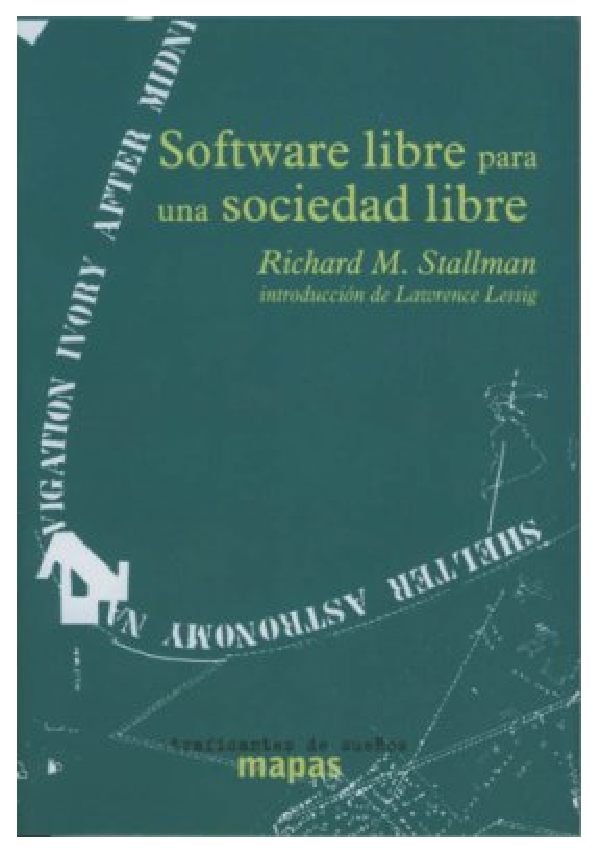
\includegraphics{portada_img}
   \end{center}
%  \vskip 0.1cm
  \begin{center}
    \normalfont\large\@date\par
  \end{center}
  \vfil
  \vfil
 \cleardoublepage
  }
\thispagestyle{empty}
\makeatother

\title{Software libre para una sociedad libre}
\author{Richard M. Stallman \\ \normalsize{Introducci�n de Lawrence Lessig}}
\date{Diciembre 2004 \\ Versi�n 1.0}
\begin{document}
\maketitle
% fin portada

% pagina de cr�ditos
\thispagestyle{empty}

\vspace*{5cm}
\noindent \textbf{Software libre para una sociedad libre} \\
Richard M. Stallman

\vspace{8mm}

\footnotesize

\noindent T�tulo original: \textit{Free Software, Free Society: Selected
Essays of Richard M. Stallman} (GNU Press, 2002) \\
Primera edici�n en castellano (en papel): Noviembre 2004 \\

\noindent Traducci�n principal: Jaron Rowan, Diego Sanz Paratcha y Laura
Trinidad \\

\noindent Edici�n: Traficantes de Sue�os \\
\noindent c/ Hortaleza 19, 1� Dcha. \\
\noindent 28004 Madrid. Tlfno: +34 1 5320928 \\
\noindent http://traficantes.net

\medskip

\noindent
\textcopyright~ Copyright 2004 de los art�culos de este libro, 
Richard M. Stallman \\   
\noindent
\textcopyright~ Copyright 2004 de la Introducci�n, Lawrence Lessig \\
\noindent
\textcopyright~ Copyright 2004 de la Edici�n, Traficantes de Sue�os

\bigskip

\noindent
Se permite la copia, ya sea de uno o m�s art�culos completos de esta obra o
del conjunto de la edici�n, en cualquier formato, mec�nico o digital, siempre
y cuando no se modifique el contenido de los textos, se respete su autor�a y
esta nota se mantenga.

\bigskip

\noindent ISBN: 84-933555-1-8 \\
\noindent Dep�sito Legal: M-44298-2004

\bigskip

\noindent \textit{Edici�n digital a cargo de:} Miquel Vidal
<miquel@barrapunto.com>. Esta edici�n electr�nica se 
ha realizado �ntegramente con software libre, mediante el 
procesador \LaTeXe{}, GNU Emacs y AUC\TeX{}.


%fin pagina de creditos

\newpage

\normalsize

% pagina de presentacion TdS
\vspace*{8cm}

\noindent \Huge\texttt{Traficantes de Sue�os}

\vspace{2cm}
\normalsize

\noindent \textsf{\mdseries \slshape
Traficantes de Sue�os no es una casa editorial, ni siquiera una editorial
independiente que contempla la publicaci�n de una colecci�n variable de
textos cr�ticos. Es, por el contrario, un proyecto, en el sentido estricto de
<<apuesta>>, que se dirige a cartograf�ar las l�neas constituyentes de otros
�rdenes de vida. La construcci�n te�rica y pr�ctica de la caja de herramientas
que, con palabras propias, puede componer el ciclo de luchas de las pr�ximas
d\'{e}cadas.}

\medskip

\noindent \textsf{\mdseries \slshape
Sin complacencias con la arcaica sacralidad de la cultura, sin concesiones
para con los narcisismos del genio literario, sin lealtad alguna a los
usurpadores del saber, TdS adopta sin ambagajes la libertad de acceso al
conocimiento. Queda, por tanto, permitida y abierta la reproducci�n total o
parcial de los textos publicados, en cualquier formato imaginable, salvo por
expl�cita voluntad del autor o de la autora y s�lo en el caso de las ediciones
con �nimo de lucro.}

\bigskip

\noindent \textsf{\mdseries \slshape \textit{Omnia sunt communia!}}




\newpage

% indice
\tableofcontents 

\thispagestyle{empty}

\newpage

% acerca
\chapter*{Acerca de la presente edici�n}

% comentado para hevea - descomentar para pdf
\fancyhead[LO,RE]{\scriptsize{Acerca de la presente edici�n}}

\addcontentsline{toc}{chapter}{Acerca de la presente edici�n}

\textsc{La presente edici�n de \textit{Software libre para una sociedad
libre}} es la primera edici�n castellana autorizada por Richard M. Stallman de
su libro Free Software, Free Society. Un exhaustivo conjunto de ensayos y
art�culos que recorren la d�cada de 1990 y los primeros a�os del nuevo
milenio, y que conforman quiz�s la mejor apolog�a escrita del software libre
como dispositivo de libertad y democracia.  El trabajo de edici�n de este
libro ha sido complejo y prolongado, y ha sido posible gracias �nicamente a la
cooperaci�n de una multitud de personas ligadas al mundo del software libre.
De este modo, el car�cter colectivo, abierto y cooperativo de la elaboraci�n
de esta edici�n guarda no pocas similitudes con los proyectos de desarrollo de
software libre.  Sin embargo, la dispersi�n de las colaboraciones y la enorme
heterogeneidad de los estilos de traducci�n ha obligado a realizar una extensa
labor de unificaci�n, en la que los criterios utilizados no son necesariamente
los preferidos por todos los traductores.  En este sentido, hemos preferido
mantener el anglicismo <<copyright>> frente al t�rmino jur�dico de <<derecho
de autor>>, m�s correcto en lengua castellana, no s�lo por el uso amplio y
extendido del t�rmino en ingl�s, sino tambi�n porque todas las referencias del
libro son a la legislaci�n estadounidense. Tambi�n hemos traducido <<library>>
por biblioteca, en lugar de librer�a, m�s extendido en el lenguaje t�cnico de
programaci�n, pero menos correcto en t�rminos de traducci�n. Por otra parte en
relaci�n a las licencias GNU de la Free Software Foundation se utiliza
indistintamente tanto la traducci�n castellana, como Licencia P�blica General
[General Public License], como las siglas inglesas por las que son m�s
corrientemente conocidas, en este caso GPL o m�s correctamente GNU GPL.

Debido a la enorme cantidad de recursos movilizados en la edici�n de esta
obra, resulta inexcusable citar y agradecer la labor de Vicente Ruiz Jurado y
Juan Carlos Gentile, que se encargaron de recopilar y coordinar las primeras
traducciones de este volumen. Tambi�n de Miquel Vidal por la orientaci�n
inicial del proyecto y desde luego, el trabajo de traducci�n inicial de:
Leovigildo Garc�a Bobadilla (introducci�n); C�sar Ballardini, Rams�s Morales,
C�sar Villanueva, �scar M\'{e}ndez Bonilla y Hugo Gayosso (cap. 1); Enrique A.
S�nchez N��ez, Diego Cadogan, Pablo Ruiz M�zquiz y de nuevo Hugo Gayosso (cap.
2); equipo de traductores al espa�ol de GNU (cap. 3); Stan Bark, Carlos Rega,
Jos� Manuel Ben�tez S�nchez, Luis M. Arteaga y Luis Bustamante (cap. 4); Pablo
Chamorro C., Steve Winston y Holman Romero (cap. 6); Steve Winston, Jos�
Manuel Ben�tez S�nchez, Ragnar Hojland Espinosa, Rams�s Morales, Esteban Osses
Anguita y Enrique A. S�nchez N��ez (cap.8); Carlos Rega y Serena Del Bianco
(cap. 11); Conrado A. Berm�dez, Viviana Cruz, Steve Winston, Luis Miguel
Arteaga y Holman Romero (cap. 14); Javier Smaldone (cap.  17); Pablo Ruiz
M�zquiz, Holman Romero e Iv�n Mart�nez Cort�s (cap. 17); Cristian Rovner y
Luis Miguel Arteaga (cap. 19); Jes�s Gonz�lez Barahona y Pedro de las Heras
Quir�s (GNU GPL); Igor Tamara, Pablo Reyes y Vladimir Tamara (GNU FDL); Rafael
Palomino (GNU LGPL); y de todos aquellos que puedan reconocer parte de su
trabajo en este libro, pero de los que nos ha sido imposible reunir sus
nombres. Por �ltimo, es necesario reconocer la cuidada labor de traducci�n y
correcci�n de los traductores principales: Jaron Rowan, Diego Sanz Paratcha y
Laura Trinidad.  Por deseo de R. M. Stallman parte de los fondos recaudados de
la venta del libro se dedicar�n a la financiaci�n de proyectos a cargo de la
Fundaci�n del Software Libre en Europa. En concreto, se destinar�n 2,5 euros
por cada ejemplar vendido. 



% prologo
\chapter*{Introducci�n}

\fancyhead[LO,RE]{\scriptsize{INTRODUCCI�N: Lawrence Lessig}}

\addcontentsline{toc}{chapter}{\textsc{Introducci�n:} Lawrence Lessig}

Cada generaci�n tiene su fil�sofo: un escritor o un artista que plasma la
imaginaci�n de una �poca. A veces estos fil�sofos son reconocidos como tales,
pero a menudo pasan generaciones antes de que se caiga en la cuenta. Sin
embargo, con reconocimiento o sin �l, cada �poca queda marcada por la gente
que expresa sus ideales, sea en el susurro de un poema o en el fragor de un
movimiento pol�tico.

Nuestra generaci�n tiene un fil�sofo. No es un artista, tampoco un escritor
profesional. Es un programador. Richard Stallman comenz� su trabajo en los
laboratorios del MIT como programador y arquitecto desarrollando software de
sistemas operativos. Ha desarrollado su carrera en la vida p�blica como
programador y arquitecto fundando un movimiento por la libertad en un mundo
cada vez m�s definido por el <<c�digo>>.

El <<c�digo>> es la tecnolog�a que hace que los ordenadores funcionen. Est�
inscrito en el software o grabado en el hardware, es el conjunto de
instrucciones, primero escritas como palabras, que dirigen la funcionalidad de
las m�quinas. Estas m�quinas (ordenadores) definen y controlan cada vez m�s
nuestras vidas. Determinan c�mo se conectan los tel�fonos y qu� aparece en el
televisor. Deciden si el v�deo puede enviarse por banda ancha hasta un
ordenador. Controlan la informaci�n que un ordenador remite al fabricante.
Estas m�quinas nos dirigen. El c�digo dirige estas m�quinas.

�Qu� control deber�amos tener sobre el c�digo? �Qu� comprensi�n? �Qu� libertad
deber�a haber para neutralizar el control que permite? �Qu� poder?

Estas preguntas han sido el reto de la vida de Stallman. A trav�s de sus
trabajos y de sus palabras nos ha incitado a ser conscientes de la importancia
de mantener <<libre>> el c�digo. No <<libre>> en el sentido de que los escritores
del c�digo no reciban una remuneraci�n, sino <<libre>> en el sentido de que el
control, que construyen los codificadores, sea transparente para todos y en el
de que cualquiera tenga derecho a tomar ese control y de modificarlo a su
gusto. Esto es el <<software libre>>, <<software libre>> es la respuesta a un
mundo construido mediante c�digo.

<<Libre>>. Stallman lamenta la ambig�edad de su propio t�rmino.\footnote{Se
refiere aqu�, por primera vez en este libro, a la doble acepci�n de la palabra
inglesa \textit{free }como libre y como gratis. [\textit{N. del E.}]} No hay
nada que lamentar. Los rompecabezas obligan a la gente a pensar y el t�rmino
<<libre>> cumple bastante bien esta funci�n de rompecabezas. Para los o�dos
estadounidenses modernos, <<software libre>> suena ut�pico, imposible. Nada,
ni siquiera el almuerzo, es libre. �C�mo podr�an ser <<libres>> las m�s
importantes palabras que dirigen las m�quinas m�s esenciales que dirigen el
mundo? �C�mo podr�a una sociedad en su sano juicio aspirar a semejante ideal?

Sin embargo, el peculiar ta�ido de la palabra <<libre>> depende de nosotros y
no del propio t�rmino. <<Libre>> tiene diferentes significados, s�lo uno de
ellos se refiere a <<precio>>. Un significado de <<libre>> mucho m�s
fundamental es, dice Stallman, el del t�rmino <<libertad de expresi�n>> o
quiz�s mejor el de la expresi�n <<trabajo libre no forzado>>. No libre como
gratuito, sino libre en el sentido de limitado en cuanto a su control por los
otros. Software libre significa un control que es transparente y susceptible
de modificaci�n, igual que las leyes libres, o leyes de una <<sociedad
libre>>, son libres cuando hacen su control cognoscible y abierto a la
modificaci�n. La intenci�n del <<movimiento software libre>> de Stallman es
producir c�digo en la medida en que pueda ser transparente y susceptible de
modificaci�n haci�ndolo <<libre>>.

El mecanismo para este fin es un instrumento extraordinariamente inteligente
llamado <<copyleft>> que se implementa a trav�s de una licencia llamada GPL.
Usando el poder del copyright, el <<software libre>> no s�lo asegura que
permanece abierto y susceptible de modificaci�n, sino tambi�n que otro
software que incorpore y use <<software libre>> ---y que t�cnicamente se
convierta en <<obra derivada>>--- debe tambi�n, a su vez, ser libre. Si uno
usa y adapta un programa de software libre y distribuye p�blicamente esa
versi�n adaptada, la versi�n distribuida debe ser tan libre como la versi�n de
la que procede. Debe hacerse as�, de lo contrario se estar� infringiendo el
copyright.

El <<software libre>>, como las sociedades libres, tiene sus enemigos.
Microsoft ha entablado una guerra contra la GPL, alertando a quienquiera que
le escuche de que la GPL es una licencia <<peligrosa>>. El peligro a que se
refiere, sin embargo, es en gran medida ficticio. Otros plantean objeciones a
la <<coerci�n>> que supone el mandato de la GPL de que las versiones
modificadas sean tambi�n libres. Pero una condici�n no es coerci�n. Si no es
coerci�n que Microsoft no permita a lo usuarios distribuir versiones
modificadas de Office sin pagarle (presumiblemente) millones, entonces no es
coerci�n que la GPL establezca que las versiones modificadas del software
libre sean tambi�n libres.

Tambi�n est�n los que califican el mensaje de Stallman de demasiado
extremista. Pero no es extremista. Al contrario, en un sentido obvio el
trabajo de Stallman es una simple traslaci�n de la libertad que nuestra
tradici�n ha inscrito en el mundo anterior al c�digo. El <<software libre>>
asegura que el mundo gobernado por el c�digo es tan <<libre>> como nuestra
tradici�n que construy� el mundo anterior al c�digo.

Por ejemplo: una <<sociedad libre>> est� regulada por leyes. Pero hay l�mites
que cualquier sociedad libre pone a esa regulaci�n legal: ninguna sociedad que
mantenga sus leyes en secreto podr�a llamarse, nunca, libre. Ning�n gobierno
que esconda sus normas a los gobernados podr�a incluirse, nunca, en nuestra
tradici�n. El Derecho gobierna. Pero s�lo, precisamente, cuando lo hace a la
vista. Y el Derecho s�lo est� a la vista cuando sus t�rminos pueden ser
conocidos por los gobernados o por los agentes de los gobernados ---abogados,
parlamentos.

Esta condici�n del Derecho va m�s all� del trabajo de un parlamento. Pensemos
en la pr�ctica jur�dica en los tribunales norteamericanos. Los abogados son
contratados por sus clientes para defender los intereses de esos clientes. En
ocasiones esos intereses son defendidos en un litigio. En el curso del
litigio, los abogados redactan alegaciones. Esas alegaciones, a su vez,
afectan a las decisiones judiciales. Esas decisiones determinan quien gana un
caso concreto o si una determinada ley guarda conformidad con una
constituci�n.

Todos los elementos de ese proceso son libres en el sentido a que se refiere
Stallman. Las alegaciones jur�dicas est�n disponibles para su libre uso por
los dem�s. Las argumentaciones son transparentes ---lo cual es distinto a
decir que son buenas--- y el razonamiento puede ser utilizado sin la
autorizaci�n del abogado original. Las opiniones formuladas pueden ser citadas
en alegaciones posteriores. Pueden ser copiadas e incorporadas en otra
argumentaci�n u opini�n. El <<c�digo fuente>> del Derecho estadounidense es
deliberadamente y por principio abierto y de libre uso por cualquiera. Y as�
lo usan libremente los abogados, ya que el secreto de una gran argumentaci�n
es que resulte original mediante la reutilizaci�n de lo que se ha hecho antes.
La fuente es libre, la creatividad y una forma de econom�a se cimentan sobre
ella.

Esta econom�a del c�digo abierto ---y me refiero aqu� al c�digo legal
abierto--- no arruina a los abogados. Las firmas de abogados tienen incentivos
suficientes para redactar buenas alegaciones incluso cuando material que crean
pueda ser apropiado y utilizado por cualquier otro. El abogado es un artesano
cuyo trabajo es de dominio p�blico. Sin embargo la artesan�a no es caridad.
Los abogados cobran, la gente no contrata ese tipo de trabajo sin un precio.
Pero esa econom�a progresa con trabajos posteriores que se a�aden a los
anteriores.

Podr�amos imaginar una pr�ctica jur�dica que fuese diferente, alegaciones y
argumentaciones que se mantuviesen secretas, sentencias que hiciesen p�blica
su decisi�n pero no sus fundamentos. Leyes que fueran guardadas por la polic�a
y no se hiciesen p�blicas para nadie m�s. Normativas que se aplicasen sin
explicar su contenido.

Podemos imaginar esa sociedad, pero no podemos imaginarnos llamarla <<libre>>.
Est�n, o no, mejor o m�s eficientemente gestionados los incentivos en esa
sociedad, esta no podr�a ser considerada libre. Los ideales de libertad, de
vida en una sociedad libre, exigen algo m�s que una gesti�n eficiente. En
cambio, el aperturismo y la transparencia son los l�mites en los cuales se
construye un sistema legal, sin que se a�adan nuevas ideas a conveniencia de
los l�deres. La vida sometida al c�digo inform�tico no deber�a ser menos.

Escribir c�digos no es pleitear. Es mejor, m�s rico, m�s productivo. Pero el
Derecho es un ejemplo obvio de que la creatividad y la motivaci�n no dependen
de un perfecto control sobres los productos que se crean. Igual que el jazz, o
las novelas, o la arquitectura, el Derecho se construye sobre el trabajo hecho
con anterioridad. La creatividad siempre es esta agregaci�n y cambio. Y una
sociedad libre es aquella que garantiza que sus recursos m�s importantes
permanecen libres, precisamente en este sentido.

Por primera vez este libro recoge los art�culos y las conferencias de Richard
Stallman de forma que queden claros su sutileza y su fuerza. Los ensayos
abarcan un amplio espectro, desde el copyright a la historia del movimiento
del software libre. Incluyen muchas argumentaciones no muy bien conocidas y,
entre ellas, una apreciaci�n especialmente inteligente sobre las cambiantes
circunstancias que vuelven sospechoso al copyright en el mundo digital.
Servir�n como recurso para aquellos que busquen comprender el pensamiento de
este hombre poderoso, poderoso por sus ideas, su pasi�n y su integridad, a
pesar de carecer de poder en los dem�s sentidos. Inspirar�n a aquellos que
adopten estas ideas y construyan a partir de ellas.

No conozco bien a Stallman. Lo conozco lo suficientemente bien para saber que
es una persona que es dif�cil que nos guste. Es obstinado, a menudo
impaciente. Su ira puede inflamarse ante un amigo con tanta facilidad como
ante un enemigo. Es testarudo y persistente, paciente en todo caso.

Pero cuando nuestro mundo finalmente comprenda el poder y el peligro del
c�digo, cuando finalmente vea que el c�digo, como las leyes o como el
gobierno, debe ser transparente para ser libre, entonces volveremos la mirada
a este programador testarudo y persistente y reconoceremos la idea por cuya
realidad ha luchado: la idea de un mundo donde la libertad y el conocimiento
sobreviven al compilador. Y comprenderemos que nadie, por medio de sus actos o
de sus palabras, ha hecho tanto para hacer posible la libertad que la sociedad
venidera podr�a tener.

A�n no hemos ganado esa libertad. Podr�amos fracasar en su consecuci�n. Pero
triunfemos o fracasemos, en estos art�culos se refleja lo que esa libertad
podr�a ser. Y en la vida que plasman esas palabras y obras est� la inspiraci�n
para todo el que, como Stallman, lucha para crear esa libertad. 

\bigskip

\begin{flushright} \noindent\textsc{Lawrence Lessig} \\ 
\textit{Presidente de Creative Commons}
\end{flushright}



\thispagestyle{empty}
\newpage

% cabeceras normales
\fancyhead[LO,RE]{\scriptsize{\leftmark}}

% seccion uno
\part{El proyecto GNU y el software libre}

\chapter[El Proyecto GNU]{El Proyecto GNU\protect\footnote{Publicado
originalmente en el libro colectivo \textit{Open Sources: Voice from the Open
Source Revolution}, O'Reilly, 1999}}


\section{La primera comunidad que comparte software}

Cuando entr� a trabajar en el Laboratorio de Inteligencia Artificial (AI Lab)
del MIT en 1971, pas� a formar parte de una comunidad que compart�a software y
llevaba haci�ndolo durante a�os. El acto de compartir software no se
circunscribe a nuestra comunidad en particular: es tan antiguo como los
propios ordenadores, lo mismo que compartir recetas es tan viejo como la
cocina. Simplemente, nosotros lo hac�amos en mayor medida. 

En el AI Lab se utilizaba un sistema operativo de tiempo compartido llamado
ITS (\textit{Incompatible Timesharing System}), dise�ado y escrito por los
hackers de la plantilla del lab en lenguaje ensamblador para el Digital
PDP-10, uno de los ordenadores m�s grandes de la �poca. Como miembro de esta
comunidad y hacker de sistemas para el AI Lab, mi labor consist�a en mejorar
dicho sistema.

No llam�bamos <<software libre>> a nuestro software porque el t�rmino no exist�a
todav�a; pero era exactamente eso. Cuando alguien de otra universidad o de
otra empresa quer�a instalar y utilizar un programa, se lo prest�bamos de buen
grado. Si descubr�as a alguien utilizando un programa poco habitual e
interesante, siempre pod�as preguntarle por el c�digo fuente, leerlo,
modificarlo o canibalizar partes de �l para montar un programa nuevo.

El uso de la palabra <<hacker>> para definir al <<que rompe sistemas de
seguridad>> es una confusi�n promovida por los medios de masas. Nosotros, los
hackers, nos negamos a reconocer esta acepci�n y seguimos utilizando este
t�rmino para describir a <<alguien que ama la programaci�n y disfruta
explorando nuevas posibilidades>>.\footnote{Resulta dif�cil dar con una definici�n sencilla de algo tan variado como es
 el \textit{hacking}, pero creo que lo que la mayor parte de los hackers
 tienen en com�n es la pasi�n l�dica, la inteligencia y la voluntad de
 exploraci�n. Podemos decir que el \textit{hacking} significa explorar los
 l�mites de lo posible con un esp�ritu de sagacidad imaginativa. Cualquier
 actividad en la que se despliegue esta sagacidad tiene <<valor>> para el
 hacker. Puedes ayudar a subsanar este malentendido haciendo una simple
 distinci�n entre la intromisi�n en la seguridad de un sistema y las
 actividades de \textit{hacking}, empleando el t�rmino \textit{cracking} para
 la primera. Quienes se dedican a esto se denominan \textit{crackers}. Es
 posible que un cracker sea tambi�n hacker, o ajedrecista, o golfista; pero la
 mayor�a no lo son (<<On Hacking>>, RMS; 2002).}


\section{EL colapso de la comunidad}

La situaci�n cambi� dr�sticamente a principios de los a�os ochenta, con la
desaparici�n de la comunidad hacker del AI Lab, seguida de la desaparici�n del
ordenador PDP-10. 

En 1981, la empresa pionera Symbolics contrat� a casi todos los hackers del AI
Lab, y nuestra diezmada comunidad fue incapaz de sobrevivir. (En el libro
\textit{Hackers}, Stephen Levy describe estos acontecimientos, a la vez que
nos proporciona un panorama bastante preciso de lo que fue la �poca dorada de
esta comunidad). Cuando el AI Lab compr� un nuevo PDP 10 en 1982, sus
administradores decidieron usar un sistema de Digital de tiempo compartido no
libre en lugar del ITS en la nueva m�quina.

Poco despu�s, Digital dej� de fabricar la serie PDP-10. Su arquitectura
elegante y poderosa de los a�os sesenta no pod�a adaptarse de forma natural a
los grandes espacios de direccionamiento caracter�sticos de los a�os ochenta.
Lo cual explica que casi todos los programas que integraban el sistema ITS
resultaran obsoletos. De esa manera se enterraba definitivamente al ITS:
quince a�os de trabajo tirados por la borda.

Los modernos ordenadores de la �poca, como el VAX o el 68020, contaban con su
propio sistema operativo, pero ninguno utilizaba software libre. Hab�a que
firmar un acuerdo de confidencialidad incluso para obtener una copia
ejecutable.

Todo ello significaba que antes de poder utilizar un ordenador ten�as que
prometer no ayudar a tu vecino. Quedaban as� prohibidas las comunidades
cooperativas. Los titulares de software propietario establecieron la siguiente
norma: <<Si compartes con tu vecino, te conviertes en un pirata. Si quieres
hacer alg�n cambio, tendr�s que rog�rnoslo>>.

La idea de que el sistema social en torno al software propietario ---un
sistema que te impide compartir o modificar el software--- es antisocial, poco
�tico, sencillamente equivocado, puede sorprender a algunos lectores. Pero
�qu� podemos decir acerca de un sistema que siembra la divisi�n entre el
p�blico y abandona a los usuarios a la indefensi�n m�s absoluta? Estos
lectores probablemente hayan asumido el sistema social asociado con el
software propietario como algo inevitable o habr�n considerado la cuesti�n de
la misma forma que se plantea por parte de las empresas de software
propietario. Los editores de software se han esforzado mucho en convencernos
de que s�lo hay una forma de abordar esta cuesti�n.

Cuando los editores de software hablan de <<ejercer>> sus <<derechos>> o de
<<acabar con la pirater�a>>, lo que dicen es, de hecho, secundario. El verdadero
mensaje de estas declaraciones se esconde en ciertas presunciones impl�citas
que dan por supuestas; creen que el p�blico debe aceptarlas sin cuestionarlas.
De modo que analic�moslas.

Una suposici�n es que las empresas de software tienen el derecho natural e
incuestionable a poseer software, y por ende a detentar todo el poder sobre
sus usuarios. (Si de verdad se tratara de un derecho natural, nosotros no
objetar�amos nada, independientemente del perjuicio que esto ocasionara al
p�blico.) Pero lo interesante es que la Constituci�n de los EE.UU. y el
derecho tradicional rechazan este punto de vista. El \textit{copyright} no es
una ley natural, sino un monopolio artificial impuesto por el Estado que
limita el derecho natural de los usuarios a copiar.

Otra presunci�n impl�cita es que lo �nico importante en el software es la
funci�n que te permite desempe�ar ---que, como usuarios de ordenadores, no
deber�amos preocuparnos de que tipo de sociedad se nos permite tener.

Una tercera presunci�n es que no dispondr�amos de software de utilidad ---o de
un programa para realizar esta u otra tarea--- si no cedemos el derecho de los
usuarios sobre un programa a la empresa responsable del mismo. Esto resultaba
convincente antes de que el movimiento del software libre demostrara que
pod�amos crear much�simos programas, y muy �tiles, sin necesidad de cadenas.



Si preferimos rechazar estas presunciones y analizamos estas cuestiones de
acuerdo con los criterios morales y el sentido com�n del ciudadano de a pie,
anteponiendo a los usuarios a cualquier otra consideraci�n, llegaremos a
conclusiones muy diferentes. Los usuarios de ordenadores deber�an ser libres
para modificar los programas y ajustarlos a sus necesidades, libres para
compartirlos, porque la cooperaci�n con los dem�s constituye la base de la
sociedad.


\section{Una elecci�n moral radical}

Una vez desapareci� mi comunidad, era imposible seguir como hasta entonces. De
modo que me enfrent� a un dilema moral radical.

Lo m�s f�cil hubiera sido subirme al tren del software propietario, firmar
acuerdos de confidencialidad y prometer no ayudar a mis compa�eros hackers. Es
muy probable que ahora me dedicara a desarrollar software publicado con
cl�usulas de confidencialidad, presionando as� a otros para traicionar tambi�n
a sus compa�eros. 

Podr�a haber ganado mucho dinero de esta forma, y quiz�s me hubiera divertido
escribiendo c�digo. Pero sab�a que, al final de mi carrera, echar�a la vista
atr�s y s�lo habr�a contribuido a levantar muros para dividir a la gente,
habr�a pasado toda mi vida convirtiendo este mundo en un lugar mucho peor.

Ya hab�a experimentado lo que se siente al firmar un acuerdo de
confidencialidad cuando una persona se neg� a entregarnos, a m� y al AI Lab,
el c�digo fuente del programa de control de nuestra impresora. (La ausencia de
ciertas funciones en este programa convert�a el uso de la impresora en una
experiencia muy frustrante.) De modo que no pod�a enga�arme sobre la inocencia
de estos acuerdos. Mont� en c�lera cuando aquel individuo se neg� a
compartirlo con nosotros. No pod�a hacerle lo mismo al resto del mundo.

Otra opci�n, m�s directa aunque desagradable, hubiera sido abandonar el mundo
de los ordenadores. De esa manera no malgastar�a mis aptitudes, aunque con
todo seguir�an sin servir de nada. No ser�a culpable de dividir y restringir
libertad a los usuarios de ordenadores, pero eso llegar�a tarde o temprano.

Decid� estudiar la manera en que un programador podr�a hacer algo por el bien
com�n. Me pregunt� si pod�a escribir uno o varios programas que permitiesen
resucitar nuevamente a nuestra extinta comunidad.

La respuesta era obvia: la primera cosa necesaria era crear un sistema
operativo, el software crucial para empezar a utilizar un ordenador. Con un
sistema operativo puedes hacer muchas cosas; sin �l, ni siquiera puedes hacer
funcionar un ordenador. Mediante un sistema operativo libre podr�amos armar
una nueva comunidad cooperativa de hackers ---e invitar a todos a que se
uniesen a ella. Y cualquiera podr�a utilizar un ordenador sin verse obligado
previamente a conspirar para privar de esto a sus amigos.

Como desarrollador de un sistema operativo, ten�a las aptitudes necesarias
para desempe�ar esta labor. De manera que, aun cuando el �xito no estuviera
asegurado, comprend� que hab�a sido elegido para llevar a cabo esta misi�n.
Opt� por crear un sistema compatible con Unix para dotarle as� de portabilidad
y facilitar el cambio a los usuarios de Unix. El nombre de GNU fue elegido
seg�n una tradici�n de los hackers, como un acr�nimo recursivo de <<GNU's Not
Unix>>.\footnote{En castellano, <<GNU No es Unix>>.}

Un sistema operativo no significa s�lo un kernel, que apenas permite ejecutar
otros programas. En los a�os setenta, cualquier sistema operativo decente
inclu�a sus propios procesadores de comandos, ensambladores, compiladores,
interpretes, depuradores, editores de textos, gestores de correo y mucho m�s.
ITS, Multics, VMS y Unix, todos inclu�an estos componentes.

M�s adelante, escuch� estas palabras, atribuidas a Hillel: <<Si no act�o en mi
nombre, �qui�n lo har� por m�? Y entonces, �en qu� me convertir�? Y si ahora
no, entonces �cu�ndo?>>.

La decisi�n de emprender el proyecto GNU se basaba en un esp�ritu similar.

Como ateo, no sigo el ejemplo de ning�n l�der religioso, pero a veces admiro
las cosas que han llegado a decir. 


\section{Libre en su acepci�n de libertad}

A veces se malinterpreta el t�rmino de <<software libre>> ---para empezar, no
tiene ninguna relaci�n con el precio. Lo que nos interesa es la libertad. He
aqu� la definici�n de software libre. Un programa es software libre para el
usuario siempre que, como usuario particular, tengas:

\begin{enumerate}

\item La libertad de ejecutar el programa sea cual sea el prop�sito.

\item  La libertad para modificar el programa para ajustarlo a tus necesidades.
(Para que se trate de una libertad efectiva en la pr�ctica, deber�s tener
acceso al c�digo fuente, dado que sin �l la tarea de incorporar cambios en un
programa es extremadamente dif�cil.)

\item La libertad de redistribuir copias, ya sea de forma gratuita, ya sea a
cambio del pago de un precio.

\item  La libertad de distribuir versiones modificadas del programa,  de tal forma
que la comunidad pueda aprovechar las mejora introducidas.

\end{enumerate}


Dado que nos referimos a la libertad y no al precio, no existe contradicci�n
alguna entre la venta de copias y el software libre. De hecho, la libertad
para vender copias es crucial: las colecciones de software libre a la venta en
formato de CD-ROM son muy importantes para la comunidad y venderlas es una
forma de recaudar fondos para el desarrollo de software libre. Por lo tanto,
cualquier programa que no podamos incluir en estas colecciones no podr�
calificarse de software libre.

Dada la ambig�edad del calificativo <<libre>>, llevamos mucho tiempo buscando
alternativas, pero nadie ha encontrado ninguna satisfactoria. La lengua
inglesa es de las m�s rica en lo que a palabras y matices se refiere, pero
carece de un t�rmino simple e inequ�voco para <<libre>> en el sentido de
libertad ---<<unfettered>> [sin cadenas] ser�a el calificativo que m�s se ajusta
al significado. Alternativas como <<liberado>>, <<libertad>> o <<abierto>> no
significan lo mismo o presentan otros inconvenientes.





\section{El software GNU y el Sistema GNU}

El desarrollo de un sistema operativo de principio a fin es un proyecto
colosal. Como primera medida, decid� adaptar y utilizar algunas piezas
existentes de software libre siempre que me fuera posible. Desde el inicio,
decid� usar \TeX como principal procesador de texto, y unos a�os m�s tarde me
pas� al X Window System en vez de escribir otro sistema de ventanas para GNU.

Debido a esta decisi�n, el sistema GNU no consiste en una colecci�n completa
de software GNU. El sistema incluye programas desarrollados por otros
individuos y para proyectos con sus propios prop�sitos que empleamos por su
condici�n de software libre.


\section{Los inicios del proyecto}

En enero de 1984 abandon� mi empleo en el MIT y comenc� a escribir
software GNU. Abandonar el MIT era imprescindible si quer�a que nadie
interfiriera en la distribuci�n de GNU como software libre. De haberme
quedado, el MIT podr�a haberse apropiado de mi trabajo e impuesto sus propios
t�rminos de distribuci�n, o incluso convertir el trabajo en un paquete de
software propietario. No ten�a ninguna intenci�n de hacer una gran cantidad de
trabajo para ver como se convert�a en algo in�til en relaci�n a su prop�sito
inicial: crear una nueva comunidad dedicada a compartir software.

No obstante, el profesor Winston, el entonces director del Lab AI en el MIT,
me invit� a utilizar las instalaciones del laboratorio.


\section{Los primeros pasos}

Poco despu�s de comenzar el proyecto GNU, me hablaron del Free University
Compiler Kit, tambi�n conocido como VUCK. [La palabra danesa para libre (free)
estaba escrita con una <<V>>] Se trataba de un compilador dise�ado para trabajar
con m�ltiples lenguajes, incluido C y Pascal, y compatible con ordenadores de
objetivos m�ltiples. Me puse en contacto con el autor para pedirle permiso y
utilizarlo en GNU.

Me contest� burlonamente, diciendo que la universidad era gratuita, pero no el
compilador. As� que decid� que el primer programa para el proyecto GNU ser�a
un compilador capaz de trabajar en m�ltiples lenguajes y plataformas.

Para evitar tener que reescribir todo el compilador, obtuve el c�digo fuente
para el compilador Pastel, un compilador de plataformas m�ltiples desarrollado
en Lawrence Livermore Lab. Soportaba, y estaba escrito, en una versi�n
ampliada de Pascal, dise�ada como lenguaje de programaci�n de sistemas. Le
a�ad� un \textit{front end} C y comenc� a pasarlo a un ordenador Motorola
68000, pero tuve que abandonar el intento al descubrir que el compilador
requer�a muchos megabytes de espacio, y el sistema Unix 68000 de entonces s�lo
ten�a capacidad para 64K.

Me di cuenta de que el compilador Pastel analizaba el archivo de entrada en
forma de �rbol sint�ctico, convirti�ndolo en una cadena de <<instrucciones>> y
luego generando todo el archivo de salida sin liberar espacio de
almacenamiento. As� que conclu� que tendr�a que escribir un nuevo compilador
partiendo de cero. El resultado es el compilador conocido como GCC; aunque no
contiene ning�n elemento del compilador Pastel, consegu� adaptar y utilizar el
\textit{front end} C que hab�a escrito. Pero eso fue a�os m�s tarde. Antes
trabaj� en el GNU Emacs.


\section{GNU Emacs}

Comenc� a trabajar en el GNU Emacs en septiembre de 1984, y a principios de
1985 ya pod�a ser utilizado. Esto me permiti�
comenzar a usar el sistema Unix para labores de edici�n. Dado que nunca me
interes� aprender a usar vi o ed, hasta entonces hab�a realizado mis ediciones
en otro tipo de m�quinas.

En aquel momento hab�a gente interesada en utilizar GNU Emacs, lo que plante�
el problema de la distribuci�n. Por supuesto, lo coloqu� en el servidor
an�nimo ftp del ordenador del MIT [Este ordenador, prep.ai.mit.edu, se
convirti� as� en el principal sitio ftp de distribuci�n de GNU; al
desmantelarlo a�os m�s tarde, transferimos el nombre a nuestro nuevo servidor
ftp]. Pero en aquel entonces, muchos no ten�an acceso a Internet y no pod�an
descargar una copia v�a FTP. �Qu� pod�a decirles?

Podr�a haberles dicho: <<Busca un amigo en la red y que te haga una copia>>. O
podr�a haber hecho lo mismo que hiciera con el PDP-10 Emacs original, a saber,
decirles: <<Env�ame una cinta y un SASE, y te lo devolver� por correo con una
copia de Emacs>>. Pero como no ten�a trabajo y andaba buscando la manera de
ganar dinero con el software libre, anunci� que enviar�a copias a cualquiera
interesado a cambio de ciento cincuenta d�lares. As� comenz� mi empresa de
distribuci�n de software libre, precursora de las empresas que hoy distribuyen
sistemas Linux basados en GNU.


\section{�Un programa es libre para cualquier usuario?}

Cuando un programa de software libre deja de estar en manos de su autor, esto
no significa necesariamente que siga siendo software libre para cualquiera que
se haga con una copia de �l. Por ejemplo, el software de dominio p�blico
---software sin \textit{copyright}--- es software libre, pero cualquiera puede
modificarlo y hacer una versi�n propietaria a partir de �l. Lo mismo ocurre
con muchos programas libres con copyright que se distribuyen con licencias
simples muy permisivas que autorizan el desarrollo de versiones propietarias
modificadas.

El ejemplo paradigm�tico de este problema es el X Window System. Desarrollado
en el MIT y publicado como software libre con una licencia permisiva, pronto
fue adoptado por diversas empresas inform�ticas. A�adieron X, s�lo en forma
binaria, a sus sistemas propietarios Unix, siempre acompa�ados del cl�sico
acuerdo de confidencialidad. Estas copias de X dejaron de ser software libre,
igual que Unix.

Los desarrolladores del X Window System no lo consideraron un problema---lo
esperaban y pretend�an que eso ocurriera. Su objetivo no era la libertad sino
el <<�xito>>, definido en funci�n del n�mero de usuarios. No les importaba si
�stos eran libres o no, bastaba con que fueran muchos.

Esto condujo a una situaci�n parad�jica, en la que dos maneras de medir el
grado de libertad dieron respuestas distintas a la pregunta <<�Es libre este
programa?>> Si atendemos a la libertad que proporcionaban los t�rminos de
distribuci�n del MIT, entonces la conclusi�n es que el X era software libre.
Pero si tenemos en cuenta la libertad del usuario medio de X, la respuesta es
que se trataba de software propietario. La mayor�a de los usuarios de X
utilizaban las versiones propietarias que ven�an con el sistema Unix, no la
versi�n libre.


\section{El Copyleft y la GNU GPL}

El objetivo de GNU era proporcionar libertad a los usuarios, no simplemente
ser popular. De modo que necesit�bamos idear unos t�rminos de distribuci�n que
impidieran que el software de GNU se convirtiera en software propietario. El
m�todo que empleamos se denomin� \textit{copyleft}.

Copyleft utiliza la ley de \textit{copyright}, pero d�ndole la vuelta para
servir a un prop�sito opuesto al habitual: en lugar de privatizar el software,
ayuda a preservarlo como software libre.

La idea fundamental del copyleft es que se autoriza la ejecuci�n del programa,
su copia, modificaci�n y distribuci�n de versiones modificadas, siempre que no
se a�ada ninguna clase de restricci�n a posteriori. De este modo, las
libertades cruciales que definen el <<software libre>> quedan garantizadas para
cualquiera que posea una copia; estas libertades se convierten en derechos
inalienables.

Para que el copyleft sea efectivo las versiones modificadas deber�n ser libres
tambi�n. Esto garantiza que cualquier tarea basada en nuestro trabajo se
pondr� a disposici�n de la comunidad si llegara a publicarse. Cuando los
programadores que tienen empleo se ofrecen voluntariamente a mejorar el
software GNU, s�lo el copyleft impide que sus jefes les digan: <<No pod�is
compartir esos cambios, porque vamos a utilizarlos para crear nuestra versi�n
propietaria del programa>>.

El requisito de que los cambios sean libres es esencial para garantizar la
libertad de los usuarios del programa. Las empresas que privatizaron el X
Window System incorporaron ciertos cambios para instalarlo en sus sistemas y
en su hardware. Estos cambios eran peque�os comparados con la envergadura del
sistema, pero no eran en absoluto triviales. Si estos cambios se esgrim�an
como excusa para denegar la libertad a los usuarios, cualquiera podr�a
aprovecharse de ello.

Al combinar un programa libre con un c�digo no libre se plantea un problema
similar. Esta combinaci�n acabar�a siendo inevitablemente no libre; las
libertades suprimidas en la parte no libre del programa afectar�n a �ste en su
totalidad. Autorizar este tipo de combinaciones abrir�a un boquete lo bastante
grande para hundir el barco entero. Por lo tanto, un objetivo crucial del
copyleft es tapar este boquete: cualquier cosa a�adida o combinada con un
programa copyleft, para formar una versi�n modificada deber� preservar su
condici�n de software libre y su copyleft.

Nosotros aplicamos una forma espec�fica de copyleft para la mayor parte del
software de GNU, conocida como la GNU General Public License o para abreviar
GNU GPL. Recurrimos a otros tipos de copyleft seg�n las circunstancias
espec�ficas. Tambi�n se aplica el copyleft a los manuales de GNU, pero
utilizamos una forma m�s sencilla, porque la complejidad de la GNU GPL resulta
innecesaria en estos casos.

En 1984 o 1985, Don Hopkins ---un compa�ero con mucha imaginaci�n--- me envi�
una carta. En el sobre hab�a escrito una serie de proverbios, incluido el que
sigue: <<Copyleft---quedan revocados todos los derechos>>. Emple� la palabra
<<copyleft>> para bautizar el concepto de distribuci�n que andaba desarrollando
en aquel momento.


\section{La Free Software Foundation}

A medida que aumentaba el inter�s por Emacs, otros vinieron a sumarse al
proyecto GNU, y decidimos que era el momento de volver a buscar
fuentes de financiaci�n. De este modo, en 1985 creamos la Free Software
Foundation, una organizaci�n sin �nimo de lucro dedicada al desarrollo de
software libre. La FSF tambi�n se hizo con la empresa de distribuci�n de
copias de Emacs, a lo que m�s tarde a�adir�a otros programas
\textit{libres}---no s�lo de GNU--- as� como la venta de manuales libres.

La FSF acepta donaciones, pero la mayor parte de sus ingresos siempre procedi�
de las ventas ---de copias de software libre y de otros servicios relacionados
con  �ste. En la actualidad, vende CD-Rom de c�digos fuente, CD-Rom con los
binarios, manuales cuidadosamente impresos ---con total libertad para
redistribuirlos y modificarlos--- y Deluxe Distributions ---colecciones
enteras de software adaptadas a la plataforma de elecci�n del cliente.

Los empleados de la Free Software Foundation han escrito y se han encargado
del mantenimiento de una serie de paquetes de software de GNU. Dos ejemplos
notables son la librer�a C y la shell. Todos los programas ejecutados en un
sistema GNU/Linux utilizan la librer�a C de GNU para comunicarse con Linux.
Fue desarrollada por un miembro de la plantilla de la Free Software
Foundation, Roland McGrath. La shell utilizada en la mayor�a de los sistemas
GNU/Linux se llama BASH ---acr�nimo de Bourne Again Shell---, desarrollada por
otro empleado de la FSF, Brian Fox.

Financiamos el desarrollo de estos programas porque el proyecto GNU no se
reduc�a exclusivamente a las herramientas o al entorno de desarrollo. Nuestra
meta era un sistema operativo completo, y estos programas eran necesarios para
alcanzar nuestro objetivo.

Con el nombre de <<Bourne again Shell>> pretend�amos mofarnos de la <<Bourne
Shell>>, la shell m�s com�n en Unix.


\section{Los servicios relacionados con el software libre}

La filosof�a del software libre rechaza una pr�ctica empresarial concreta y
muy generalizada, \textit{pero no rechaza el negocio} en general. Cuando una
empresa respeta la libertad de los usuarios, le deseamos mucho �xito.

La venta de copias de Emacs ilustra una clase de empresa relacionada con el
software libre. Cuando la FSF se hizo con el negocio, me vi obligado a
buscarme nuevamente la vida. As� fue como empec� a vender servicios
relacionados con el software libre que acababa de desarrollar. Esto inclu�a la
ense�anza de cuestiones como la programaci�n de GNU Emacs, la modificaci�n del
GCC a la medida del usuario o el desarrollo de software, normalmente para
instalar el GCC en nuevas plataformas.

Hoy por hoy, una serie de corporaciones se dedican a este tipo de servicios
relacionados con el software libre. Algunas distribuyen colecciones de
software libre en CD-Rom; otras proporcionan servicio t�cnico a distintos
niveles, contestando a las preguntas de los usuarios, subsanando \textit{bugs}
o a�adiendo nuevas funciones. Incluso, estamos empezando a ver empresas
dedicadas al lanzamiento de nuevos productos de software libre.

Pero debemos andarnos con cuidado ---una serie de empresas asociadas con el
t�rmino <<c�digo abierto>> basan su mercado en el software no libre que funciona
con software libre. No son empresas de software libre, su software es
propietario, y con sus productos pretenden tentar a los usuarios y despojarles
de su libertad. Se las conoce como empresas de <<valor a�adido>>, lo que refleja
los valores que querr�an que adopt�semos: la comodidad antes que la libertad.
Si valoramos la libertad, deber�amos hablar de productos de <<libertad
sustra�da>>.


\section{Los objetivos t�cnicos}

El principal objetivo de GNU era ser software libre. Aun cuando GNU no
entra�ara ninguna ventaja t�cnica frente a Unix, s� tendr�a una ventaja
social, al permitir que los usuarios cooperaran, y otra �tica, al respetar su
libertad.

Pero es natural aplicar al trabajo los criterios ya conocidos de buena
pr�ctica ---por ejemplo, la asignaci�n din�mica de estructuras de datos para
evitar las limitaciones de tama�o fijadas arbitrariamente y el empleo de
c�digos de ocho bits, siempre que esto resultara apropiado.

Por otro lado, rechaz�bamos ese empe�o de Unix en conservar una memoria
reducida, y as� decidimos no dar soporte a las m�quinas de 16 bits ---estaba
claro que las de 32 bits ser�an la norma, para cuando hubi\'{e}ramos terminado
el sistema GNU --- y no reducir la memoria a menos que super�semos un
megabyte.  En los programas en que no fuera crucial administrar archivos de
gran tama�o, anim�bamos a los programadores a insertar un archivo de entrada
entero en el core, luego a escanear su contenido sin preocuparse del I/O.

Estas decisiones permitieron que muchos programas GNU superasen a sus
hom�logos de Unix en fiabilidad y velocidad.


\section{La donaci�n de ordenadores}

A medida que iba aumentaba la popularidad del proyecto GNU, la gente empez� a
donar ordenadores que operaban con Unix. Y fueron de gran utilidad, porque la
forma m�s f�cil de desarrollar componentes de GNU era partiendo de un sistema
Unix y reemplazar sus componentes uno a uno. Pero esto nos plante� un dilema
�tico: \textit{�era correcto poseer, aunque fuera tan solo una copia, de
Unix?}

Unix era ---y es--- software propietario, y seg�n la filosof�a del proyecto
GNU no deb�amos recurrir a �l. Pero, al aplicar la misma l�gica que nos lleva
a justificar el uso de la violencia en leg�tima defensa, conclu� que era
igualmente leg�timo utilizar un paquete propietario cuando �ste resultara
crucial para desarrollar un sustituto libre que ayudar�a a otros a dejar de
utilizar el paquete propietario.

Pero, aun cuando los medios justificaran el fin, no dejaban de ser medios poco
�ticos. Hoy en d�a ya no tenemos ninguna copia de Unix, porque lo
reemplazamos por sistemas operativos libres. Cuando no pod�amos sustituir el
sistema operativo de un ordenador por otro libre, entonces reemplaz�bamos el
ordenador entero.


\section{La lista de tareas de GNU}

A medida que avanzaba el proyecto GNU y se desarrollaron o descubrieron un
creciente n�mero de componentes de sistema, nos pareci� muy �til elaborar una
lista de asignaturas pendientes. La utilizamos para reclutar desarrolladores
que escribieran las piezas que faltaban. Esta lista se conoci� como la lista
de tareas de GNU. Adem�s de los componentes de Unix, incluimos en la lista
otros proyectos �tiles de software y la documentaci�n que, en nuestra opini�n,
precisaba cualquier sistema completo.



En la actualidad, apenas figuran algunos componentes de Unix en la lista de
tareas de GNU ---hemos llevado a cabo la mayor parte, a excepci�n de algunas
menos trascendentales. Pero la lista est� repleta de proyectos que podr�an
calificarse de <<aplicaciones>>. Cualquier programa que despierte el inter�s de
algo m�s que un reducido grupo de usuarios se a�adir� al sistema operativo. 

Incluso llegamos a incluir juegos en esta lista ---lo hicimos desde
el principio. Unix conten�a juegos, as� que l�gicamente GNU ten�a que hacer lo
propio. Pero la compatibilidad nunca fue un problema para los juegos, de modo
que no replicamos los de Unix. Optamos en cambio por una gama de distintas
clases de juegos que pensamos podr�n gustar a los usuarios.


\section{La librer�a GNU GPL}

La librer�a C GNU utiliza un copyleft especial llamado GNU Library General
Public License, que autoriza el enlace de software propietario con la
librer�a. �Por qu� permitir esta excepci�n?

No es una cuesti�n de principios. Ning�n principio establece el derecho de los
productos de software propietario a incluir nuestro c�digo ---�por qu�
contribuir a un proyecto que niega el derecho a compartir? El uso de la LGPL
para la librer�a C, o para cualquier otra librer�a, responde m�s bien a una
estrategia.

La librer�a C desempe�a tareas gen�ricas; todo sistema o compilador
propietario viene acompa�ado de una librer�a C. Por lo tanto, limitar nuestra
librer�a C al software libre no reportar�a ninguna ventaja para �ste
---hubiera desalentado el uso de nuestra librer�a.

Nuestro sistema es una excepci�n a este respecto: en el sistema GNU
---incluido GNU/Linux---, la librer�a C GNU es la �nica en C. Por lo que los
t�rminos de distribuci�n de la librer�a C GNU determinan si es posible o no
compilar un programa propietario para el sistema GNU. No existen razones
�ticas para autorizar la incorporaci�n de aplicaciones propietarias en el
sistema GNU, pero estrat�gicamente parece que prohibir esto desincentivar�a el
uso del sistema GNU en lugar de alentar el desarrollo de aplicaciones libres.

Esta es la raz�n de que utilizar la Library GPL sea una buena estrategia para
la librer�a C. Para otras librer�as, la estrategia a adoptar debe estudiarse
caso por caso. Si una librer�a desempe�a una tarea especial que puede ayudar a
escribir ciertos tipo de programas, publicarla con GPL, limit�ndola
exclusivamente a los programas libres, ser� una manera de ayudar a otros
desarrolladores de software libre, proporcion�ndoles una ventaja frente al
software propietario.

Tomemos por ejemplo la GNU Readline,\footnote{La librer�a GNU Readline provee
una serie de funciones a aquellas aplicaciones que permitan a sus usuarios
editar l�neas de comando desde el teclado.} una librer�a desarrollada para la
edici�n de comandos para BASH. Readline se publica con una GNU GPL ordinaria,
no con la Library GPL. Es indudable que esto reduce el volumen de uso de
Readline, pero no supone una p�rdida para nosotros. Por otro lado, se ha
desarrollado al menos una aplicaci�n �til en software libre que puede utilizar
la Readline, y esto s� constituye un aut�ntico logro para la comunidad.

Los desarrolladores de software propietario cuentan con la ventaja que
proporciona el dinero; los de software libre deben idear ventajas
entre ellos. Espero que un d�a contemos con una amplia colecci�n de
librer�as con GPL sin paralelo en el mundo del software propietario, una
colecci�n que proporcione m�dulos �tiles que sirvan de base para el futuro
software libre y entra�en una ventaja decisiva para fomentar su desarrollo.


\section{�Un reto personal?}

Eric Raymond dice que <<todo buen trabajo de software empieza
cuando un desarrollador se plantea un reto personal>>. Es posible
que est� en lo cierto, pero muchos componentes esenciales del software GNU se
desarrollaron con el fin de crear un sistema operativo libre y completo. Su
origen est� en una visi�n y un plan, no en un impulso individual.

Por ejemplo, desarrollamos la librer�a C GNU, la Bourne Again Shell (BASH) y
el GNU tar porque cualquier sistema similar a Unix precisaba de estos
componentes. Lo mismo puede decirse de mis propios programas ---el compilador
C GNU, GNU Emacs, GDB y GNU Make.

Algunos programas GNU se desarrollaron para enfrentarse a amenazas espec�ficas
sobre nuestra libertad. Por eso desarrollamos el gzip, para sustituir al
programa Compress cuando �ste dej� de estar a disposici�n de la comunidad
gracias a las patentes LZW.\footnote{El algoritmo Lempel-Ziv-Welch se emplea
para la compresi�n de datos.} Buscamos a gente que pudiera desarrollar el
LessTif, y m�s recientemente GNOME y Harmony, y as� abordar los problemas
planteados por ciertas librer�as propietarias ---v�ase a continuaci�n
<<Librer�as no libres>>. Estamos desarrollando el GNU Privacy Guard para
reemplazar el popular software de encriptaci�n no libre, porque los usuarios
no deber�an verse obligados a elegir entre su privacidad y su libertad.

Claro que la gente encargada de escribir estos programas empez� a interesarse
en el trabajo, y algunos a�adieron muchas funciones para satisfacer sus
propias necesidades e intereses. Pero esa no es la raz�n de la existencia de
los programas.


\section{Acontecimientos inesperados}

Al iniciarse el proyecto GNU pens� que desarrollar�amos el sistema en su
totalidad y luego lo publicar�amos entero. Pero no fue as�.

Dado que cada uno de los componentes del sistema GNU se implant� en un sistema
Unix, todos ellos pod�an ejecutarse en sistemas Unix mucho antes de que
existiera el sistema GNU. Algunos de estos programas se hicieron muy populares
y los usuarios empezaron a ampliarlos y a transportarlos ---a las diversas
versiones incompatibles de Unix, y tambi�n a otros sistemas. 

El proceso dot� de mayor potencia a estos programas, y atrajo tanto fondos
como colaboradores al proyecto GNU. Pero es probable que tambi�n retrasara la
concepci�n de un sistema m�nimamente funcional durante varios a�os, dado que
los desarrolladores de GNU dedicaban la mayor parte de su tiempo al
mantenimiento de estos puertos y a la incorporaci�n de funciones a los
componentes existentes, en vez de escribir los que faltaban.


\section{El GNU Hurd}

En 1990, el sistema GNU estaba casi terminado. Faltaba crear un solo
componente central, el kernel. Decidimos crearlo como una colecci�n de
procesos de servidor que se ejecutar�a sobre Mach. Mach es un microkernel
desarrollado en la Carnegie Mellon University y, m�s tarde, en la Universidad
de Utah. El GNU Hurd es una colecci�n de servidores ---o <<manada de
gnus>>---implantados en Mach que desempe�an las diversas tareas propias del
kernel de Unix. Su desarrollo se retras� mientras esper�bamos la publicaci�n
de Mach como software libre, tal y como nos hab�an prometido.



Una de las razones que nos impuls� a elegir este dise�o era evitar lo que
parec�a la parte m�s dura del trabajo: depurar un programa de kernel sin un
depurador de fuentes. Esto ya se hab�a resuelto en Mach, y esper�bamos depurar
los servidores Hurd como programas de usuarios, con el GDB. Pero pas� mucho
tiempo hasta que lo logramos, y los servidores multiproceso que se env�an
mensajes entre s� resultan extremadamente dif�ciles de depurar. La
consolidaci�n del Hurd ha llevado much�simos a�os.


\section{Alix}

En principio, el kernel GNU \textit{no} iba a llamarse Hurd. Su nombre
original era Alix ---por mi novia de aquel momento. Ella era administradora de
sistemas Unix, y advirti� que su nombre casaba perfectamente con los nombres
escogidos para las distintas versiones de Unix. Bromeando, le dijo a sus
amigos: <<Deber�an bautizar un kernel con mi nombre>>. No dije nada, pero decid�
sorprenderla con un kernel llamado Alix.

Sin embargo, el nombre no se mantuvo. Michael Bushnell ---ahora Thomas---, el
principal desarrollador del kernel, prefer�a el nombre de Hurd, y llam� Alix a
una parte del kernel ---la encargada de capturar las llamadas del sistema y
administrarlas enviando mensajes a los servidores Hurd.

Por fin, Alix y yo nos separamos y ella se cambi� de nombre. En cualquier
caso, el dise�o de Hurd se modific� para que la librer�a C enviase mensajes
directamente a los servidores, lo que supuso la desaparici�n del componente
Alix.

Pero antes de todo esto, una amiga de Alix se encontr� con el nombre en el
c�digo fuente de Hurd y se lo cont�. As� que el nombre cumpli� su cometido.


\section{Linux y GNU/Linux}

El GNU Hurd no est� listo para producci�n. Afortunadamente, otro kernel estaba
a nuestra disposici�n. En 1991, Linus Torvalds desarroll� un kernel compatible
con Unix y lo llam� Linux. En el a�o 1992, la combinaci�n de Linux con el
incompleto sistema GNU result� en un sistema operativo libre. [Esta
combinaci�n fue, por supuesto, una labor extraordinaria]. Gracias a Linux
podemos ejecutar hoy una versi�n del sistema GNU.

Denominamos esta versi�n GNU/Linux para explicar su composici�n, una
combinaci�n del sistema GNU con Linux como kernel.


\section{Los retos futuros}

Hemos demostrado ser capaces de desarrollar una amplia gama de software libre.
Esto no significa que seamos invencibles e imparables. Existen diversos retos
que plantean un futuro incierto para el software libre. Enfrentarnos a ellos
nos exigir� un esfuerzo constante y mucha resistencia, a veces por muchos
a�os. Necesitaremos la clase de determinaci�n que exhibe la gente cuando
valora su libertad y la protege a toda costa.



En los cuatro apartados que siguen discutiremos estos retos.


\section{Hardware secreto}

Los fabricantes de hardware tienden cada vez m�s a mantener en secreto las
especificaciones del hardware. Esto dificulta enormemente la tarea de escribir
drivers libres para que Linux y Xfree86\footnote{El Xfree86 es un programa que
proporciona un entorno de escritorio que interact�a con tu hardware ---rat�n,
teclado, etc. Funciona en plataformas muy diversas.} sean compatibles con el
hardware nuevo. Hoy contamos con sistemas libres \textit{y} completos, pero no
durar�n mucho si no son compatibles con los ordenadores del ma�ana.

Hay dos formas de enfrentarse a este problema. Los programadores pueden hacer
ingenier�a inversa para descubrir c�mo crear programas compatibles con el
hardware. El resto podemos elegir qu� hardware ser� compatible con el software
libre. A medida que aumente el n�mero de usuarios de software libre, el
secretismo de estas especificaciones se convertir� en una pol�tica
contraproducente.

Hacer ingenier�a inversa es una labor colosal. �Contaremos con programadores
lo bastante decididos para llevarla a cabo? S�, siempre que les hayamos
convencido de que el software libre es una cuesti�n de principios y de que los
drivers no libres son intolerables. �Invertiremos dinero extra, e incluso
tiempo extra, para poder utilizar drivers libres? S�, siempre y cuando se
generalice esta voluntad de recuperar nuestra libertad.


\section{Librer�as no libres}

La librer�a no libre que opera en un sistema operativo libre constituye una
trampa para los desarrolladores de software libre. Las atractivas funciones de
la librer�a son el cebo perfecto; al utilizar la librer�a, caes en la trampa,
porque tu programa no puede integrarse de forma �til en un sistema operativo
libre. [Estrictamente hablando, podr�amos incluir tu programa, pero �ste no
podr�a ejecutarse sin la librer�a]. Y, lo que es peor, en caso de
popularizarse un programa que utilice una librer�a propietaria, podr�a
arrastrar a otros programadores desprevenidos hacia la misma trampa.

El primer ejemplo de este problema se present� en los a�os ochenta, con el
Motif \textit{toolkit}.\footnote{Motif es una interfaz gr�fica y administrador
de ventanas que opera en X Window, un potente sistema gr�fico basado en una
arquitectura cliente/servidor.} Aunque entonces no hab�a sistemas operativos
libres, estaba claro qu� problema iba a plantearles el Motif m�s tarde. El
Proyecto GNU respondi� de dos formas: planteando la necesidad de que los
proyectos individuales de software libre fueran compatibles tanto con los
toolkit widgets X libres como con Motif, y encargando la creaci�n de un
sustituto libre para Motif. La tarea tard� muchos a�os en concluirse. S�lo en
1997 el LessTif, desarrollado por los Hungry Programmers, fue lo
suficientemente potente para la mayor�a de las aplicaciones Motif.

Entre 1996 y 1998, otro toolkit no libre de Graphical User Interface (GUI)
llamado Qt se incorpor� a una notable colecci�n de software libre, el
escritorio KDE.

Los sistemas libres GNU/Linux no pod�an aprovechar el KDE porque no pod�amos
emplear la librer�a. A pesar de ello, algunos distribuidores comerciales de
sistemas GNU/Linux, bastante flexibles a la hora de mezclar software
libre, a�adieron el KDE a sus sistemas ---lo cual dar�a lugar a un sistema con
m�s posibilidades y menos libertad. El grupo KDE anim� activamente a otros
programadores a que utilizasen Qt, mientras que millones de nuevos <<usuarios
de Linux>> ni siquiera sospechaban que pudiera existir un problema al respecto.
La situaci�n era desoladora.

La comunidad del software libre reaccion� de dos maneras: GNOME y Harmony.

GNOME, el GNU Network Object Model Environment, es el proyecto de escritorio
de GNU. Miguel de Icaza tom� la iniciativa en 1997, y se desarroll� con el
apoyo de Red Hat Software. GNOME pretend�a proveer prestaciones similares,
pero usando exclusivamente software libre. Entra�a algunas ventajas t�cnicas,
como la de ser compatible con varios lenguajes, y no s�lo el C++. Pero su
principal prop�sito era la libertad, funcionar sin software no libre.

Harmony es una librer�a sustitutiva compatible, dise�ada con el fin de
ejecutar software KDE sin recurrir a Qt.

En noviembre de 1998, los desarrolladores de Qt anunciaron un cambio de
licencia que, en caso de aplicarse, lo convertir�a en software libre. Aunque
no podemos estar seguros de esto, creo que el cambio se debi� en parte a la
firme respuesta de la comunidad ante el problema que planteaba la condici�n no
libre de Qt. [Esta nueva licencia es inc�moda y no equitativa, por lo que
sigue siendo aconsejable evitar el uso de Qt\footnote{En septiembre de 2000
volver�a a publicarse el Qt con GNU GPL, lo que b�sicamente resolv�a el
problema.}]

�C�mo responderemos a la tentaci�n que plantee la pr�xima librer�a no libre?
�Comprender� la comunidad la necesidad de mantenernos alejados de cualquier
trampa que se nos presente en el camino? �O renunciaremos a la libertad a
cambio de la comodidad, y dar lugar as� a un problema mucho mayor? Nuestro
futuro depende de nuestra filosof�a.


\section{Patentes de software}

La amenaza m�s seria a la que nos enfrentamos procede de las patentes de
software, que pueden introducir algoritmos y funciones fuera del alcance del
software libre al menos durante veinte a�os. Las patentes del
algoritmo de compresi�n LZW se aplicaron en 1983, y todav�a no podemos
publicar software libre que produzca GIFs adecuadamente comprimidos. En 1998,
se suspendi� la distribuci�n de un programa libre para producir archivos de
audio MP3 comprimidos bajo amenaza de una demanda judicial por
patente.

Existen formas de abordar la cuesti�n de las patentes: buscar pruebas que
demuestren la invalidez de una patente o buscar modos alternativos
para realizar una tarea. Pero estos m�todos funcionan s�lo de vez en cuando;
cuando fallan ambos, la patente puede resultar en un software libre
desprovisto de alguna funci�n necesaria para los usuarios. �Qu� haremos
entonces?

Quienes valoramos el software libre por la libertad que �ste entra�a
seguiremos en la misma l�nea. Lograremos sacar adelante el trabajo sin
funciones patentadas. Pero quienes valoran el software libre porque esperan
que sea t�cnicamente superior se inclinar�n por calificarlo de fracaso cuando
este software se vea restringido por una patente. De modo que, a pesar de que
resulta muy �til discutir la efectividad pr�ctica del modelo de desarrollo de
tipo <<catedral>> y la fiabilidad y potencia de ciertos programas de software
libre, debemos ir m�s all�. Debemos hablar de libertad y de principios.


\section{Documentaci�n libre}

La mayor deficiencia de nuestros sistemas operativos no reside en el software,
sino en la ausencia de buenos manuales libres para nuestros sistemas. La
documentaci�n es una parte esencial de cualquier paquete de software; un
paquete importante de software libre sin un buen manual libre que lo acompa�e
constituye un lastre considerable. Tenemos muchos ejemplos de ello en la
actualidad.

La documentaci�n libre, al igual que el software, es una cuesti�n de libertad,
no de precio. Los criterios para el manual libre son bastante parecidos a los
del software libre: hay que darles a los usuarios ciertas libertades. Debe
autorizarse la redistribuci�n ---incluida la venta comercial--- en papel y
\textit{on line}, de modo que el manual pueda acompa�ar a todas las copias del
programa.

Autorizar su modificaci�n resulta igualmente crucial. Por regla general, no
creo que la gente deba tener el derecho de modificar toda clase de art�culos y
libros. Por ejemplo, no creo que ni t� ni yo estemos obligados a autorizar la
modificaci�n de art�culos como este, que describe nuestros actos y opiniones.

Pero existe una raz�n espec�fica de que la libertad para modificar sea un
elemento crucial para la documentaci�n relativa al software libre. Cuando los
individuos ejercen su derecho a modificar el software, y a�adir o cambiar sus
funciones, si son lo bastante concienzudos cambiar�n asimismo el manual ---y
as� proporcionar�n una documentaci�n concisa y �til junto con el programa
modificado. Un manual que no permita a los programadores trabajar
concienzudamente y terminar su labor no satisfar� las necesidades de la
comunidad.

Algunos l�mites a la incorporaci�n de estas modificaciones no plantean
problema alguno, como es el caso de los requisitos establecidos para preservar
la advertencia sobre \textit{copyright} del autor original, los t�rminos de
distribuci�n o la lista de autores. O aquellos que exigen que las versiones
modificadas incluyan la fecha de la modificaci�n, o que incluso proh�ben la
supresi�n o alteraci�n de secciones enteras, siempre que �stas no traten sobre
temas t�cnicos. Este tipo de restricciones no plantean un problema porque no
impiden al programador concienzudo adaptar el manual para que se ajuste al
programa modificado. Dicho de otro modo, no impiden que la comunidad de
software libre disfrute plenamente del uso del manual.

Sin embargo, debemos ser capaces de modificar el contenido <<t�cnico>> del
manual y luego distribuir el resultado en los medios y canales habituales; de
lo contrario, las restricciones obstruir�n a la comunidad, el manual dejar� de
ser libre y necesitaremos elaborar uno nuevo.

�Contar�n los desarrolladores de software libre con la conciencia y la
determinaci�n para producir una amplia gama de manuales libres? Una vez m�s,
nuestro futuro depende de nuestra filosof�a.


\section{Es necesario hablar de libertad}

Actualmente, se calcula que existen diez millones de usuarios de sistemas
GNU/Linux como Debian GNU/Linux y Red Hat Linux. El software libre ha
desarrollado tales ventajas pr�cticas que est� ganando adeptos por razones
puramente pr�cticas.

Las consecuencias positivas de esto son evidentes: un mayor inter�s por
desarrollar software libre, m�s clientes para las empresas de software libre y
una mayor capacidad para alentar a las empresas a desarrollar software libre
comercial en lugar de productos de software propietario.

Pero el inter�s en el software crece a un ritmo superior que la conciencia de
la filosof�a en que se fundamenta, y esto plantea ciertas dificultades.
Nuestra capacidad para hacer frente a los desaf�os y las amenazas
anteriormente descritos depender� de nuestra voluntad de mantenernos firmes en
nombre de la libertad. Para convencer de ello a nuestra comunidad, habremos de
difundir la idea entre los nuevos usuarios que pasen a formar parte de ella.

Pero estamos fracasando: nuestros esfuerzos por atraer a nuevos usuarios a
nuestra comunidad superan con creces a nuestras iniciativas a la hora de
ense�arles los principios de nuestra comunidad. Debemos dedicarnos a ambos
objetivos y compensar nuestros esfuerzos en ambas direcciones.


\section{<<Open Source>> (c�digo fuente abierto)}

La tarea de ense�ar a los nuevos usuarios el valor de la libertad se complic�
especialmente en 1998, cuando parte de la comunidad decidi� abandonar el
t�rmino <<software libre>> y empez� a hablar de <<software de c�digo abierto>>.

Los partidarios de este t�rmino trataban de evitar la confusi�n entre <<libre>>
y <<gratuito>>---un objetivo muy leg�timo. Pero otros intentaban dejar a un lado
los principios que hab�an impulsado la creaci�n del software libre y el
proyecto GNU, procurando as� atraer a los ejecutivos y a los usuarios de
empresas, quienes comparten mayoritariamente una ideolog�a que antepone las
ganancias econ�micas a la libertad, a la comunidad, a los principios. De modo
que la ret�rica del <<c�digo abierto>> se concentra en la posibilidad de crear
un software de alta calidad y capacidad, pero rehuye las nociones de libertad,
comunidad y principios.

Un claro ejemplo de ello son las revistas <<Linux>> ---est�n repletas de
anuncios de software propietario que funciona con GNU/Linux. Cuando aparezca
el pr�ximo Motif, o Qt, �advertir�n estas revistas a los programadores de
que se alejen de ellos, o los anunciar�n sin m�s?

El apoyo de la comunidad empresarial puede contribuir al bien de la comunidad
de distintas maneras, siempre que partamos de unas condiciones de igualdad.
Pero si nos ganamos su apoyo call�ndonos lo que pensamos sobre la libertad y
los principios, el resultado puede ser desastroso, y s�lo se agudizar�a el
desequilibrio ya existente entre la difusi�n y la educaci�n c�vica.

Los t�rminos <<software libre>> y <<c�digo abierto>> describen m�s o menos la
misma categor�a de software, pero implican cosas muy distintas acerca del
software y sus valores. El Proyecto GNU sigue empleando el t�rmino <<software
libre>> para expresar la idea de que la libertad, y no s�lo la tecnolog�a, es
importante.





\section{�Int�ntalo!}

La filosof�a de Yoda ---<<No podemos s�lo intentarlo>>--- suena bien, pero no
me sirve. He realizado mi trabajo siempre ansioso ante la perspectiva de que
no tuviera suficiente capacidad para ello, sin saber si mi labor bastar�a para
alcanzar el objetivo deseado. Pero lo intent� de todas formas, porque entre el
enemigo y mi ciudad s�lo estaba yo. Para mi sorpresa, a veces del �xito
obtenido.

En otras ocasiones fracas�. Algunas de mis ciudades han ca�do. M�s tarde
descubr� otra ciudad amenazada y me prepar� para otra batalla. Con el tiempo,
he aprendido a detectar las amenazas y a interponerme entre ellas y mi ciudad,
haciendo un llamamiento a otros hackers para unirse a m�.



Hoy en d�a, a menudo me encuentro que no estoy solo. La visi�n de un
regimiento de hackers manos a la obra constituye una fuente de alivio y de
alegr�a, y pienso que la ciudad sobrevivir� por el momento. Pero con el
transcurso de los a�os los peligros son cada vez mayores, y ahora Microsoft
nos tiene en su punto de mira. No podemos pensar que el futuro de la libertad
est� asegurado. �No os enga��is! Si quieres conservar tu libertad, tienes que
estar preparado para defenderla.


\chapter[El Manifiesto GNU]{El Manifiesto GNU\protect\footnote{Publicado por
primera vez en 1984}}

\textit{El Manifiesto GNU fue escrito por Richard Stallman en los comienzos
del Proyecto GNU, con el fin de pedir participaci�n y apoyo. En los primeros
a�os, se hicieron actualizaciones menores para tomar en cuenta nuevos
desarrollos, pero ahora parece ser mejor dejarlo como esta tal y como la
mayor�a de la gente lo ha visto. Desde entonces, hemos aprendido que es
posible ayudar a evitar ciertas confusiones corrientes con un cambio en la
selecci�n de palabras, a lo largo de estos se han a�adido notas al pie de
p�gina para aclarar estas confusiones}.



\section{�Qu� es GNU? �Gnu No es Unix!}

GNU, que significa Gnu No es Unix, es el nombre de un sistema de software
completamente compatible con Unix que estoy escribiendo para poder
regalarlo\footnote{Esta expresi�n era desafortunada. La intenci�n era decir
que nadie tendr�a que pagar por el \textit{permiso} de usar el sistema GNU.
Pero las palabras no aclaran, y la gente interpreta a menudo que se dice que
las copias de GNU deber�n ser siempre distribuidas a un costo bajo o sin
costo. �sta nunca fue la intenci�n; m�s adelante, el manifiesto menciona la
posibilidad de que las compa��as provean servicios de distribuci�n con una
ganancia. Con posterioridad he aprendido a distinguir cuidadosamente entre
<<free>> [libre] en el sentido de libertad y <<free>> [gratis] en el sentido
del precio. Software libre es software que los usuarios tienen la libertad de
distribuir y cambiar. Algunos usuarios pueden obtener copias sin pagar,
mientras que otros pagan para obtener copias; y si los fondos ayudan a apoyar
la mejora del software, tanto mejor. Lo importante es que todos los que tengan
una copia tengan la libertad de cooperar con otros al usarlo.} libremente a
quien pueda utilizarlo. Hay varios voluntarios ayud�ndome. Son muy necesarias
las contribuciones en tiempo, dinero, programas y equipamiento.

Hasta el momento tenemos un editor de texto Emacs con Lisp para escribir
comandos de edici�n, un depurador de c�digo fuente, un generador compatible
con yacc, un comunicador y alrededor de 35 utilidades. Un shell (int�rprete de
comandos) se encuentra casi terminado. Un nuevo compilador portable de C ha
sido compilado y ser� lanzado este a�o. Existe un kernel inicial pero requiere
muchas m�s caracter�sticas para emular a Unix. Cuando el n�cleo y el
compilador est�n completos, ser� posible distribuir un sistema GNU apropiado
para el desarrollo de programas. Usaremos el procesador de documentos TeX,
pero tambi�n se est� trabajando en un nroff. Usaremos tambi�n el sistema libre
de ventanas X que se puede migra. Despu�s de esto agregaremos un Lisp
portable, un juego Empire, una hoja de c�lculo y cientos de otras cosas,
adem�s de documentaci�n en l�nea. Esperamos proporcionar, con el tiempo, todas
las utilidades que vienen normalmente con un sistema Unix, y m�s.

GNU ser� capaz de ejecutar programas de Unix, pero no ser� id�ntico a Unix.
Haremos todas las mejoras que sean convenientes y est�n basadas en nuestra
experiencia con otros sistemas operativos. Concretamente, planeamos tener
nombres de archivos m�s largos, n�meros de versi�n de archivos, un sistema de
archivos a prueba de ca�das, tal vez incorporemos un sistema para completar
nombres de archivos, soporte en pantalla independiente del tipo de terminal y
quiz� en un futuro un sistema de ventanas basado en Lisp a trav�s del cual
varios programas Lisp y programas ordinarios Unix puedan compartir una sola
pantalla. Tanto C como Lisp estar�n disponibles como lenguajes de
programaci�n. Intentaremos soportar UUCP, Chaosnet del MIT y otros protocolos
para comunicaci�n en Internet.

GNU est� siendo escrito inicialmente para m�quinas de la clase 68000/16000 con
memoria virtual, porque �stas son las m�quinas en las que es m�s sencilla su
ejecuci�n. El esfuerzo adicional para hacerlo funcionar en m�quinas m�s
peque�as se dejar� a alguien que quiera utilizarlo en ellas.

Para evitar una horrible confusi�n, por favor pronuncie la <<G>> en la palabra
<<GNU>> cuando se refiera al nombre de este proyecto.\footnote{GNU se
pronuncia en ingl�s de forma muy similar a \footnote{new}, que significa
<<nuevo>>. [\textit{N. del E.}]}


\section{Por qu� debo escribir GNU}

Considero que la regla de oro requiere que si a mi me gusta un programa, lo
debo compartir con otra gente que le guste. Los vendedores de software quieren
dividir a los usuarios y seducirlos, haciendo que cada usuario acuerde no
compartir su software con otros. Yo reh�so a romper mi solidaridad con otros
usuarios de esta manera. No puedo en buena conciencia firmar un acuerdo de no
divulgaci�n o un acuerdo de licencia de software. Durante a�os trabaj� dentro
del Laboratorio de Inteligencia Artificial para impugnar estas tendencias y
otras descortes�as, pero al final ellos fueron demasiado lejos: no pod�a
permanecer en una instituci�n donde hiciera estas cosas en contra de mi
voluntad.

De manera que para poder continuar usando ordenadores sin verg�enza, he
decidido agrupar un cuerpo suficiente de software libre de tal manera que
pueda seguir andando sin ninguna clase de software que no sea libre. He dejado
el laboratorio de IA para negar al MIT cualquier excusa legal que me proh�ba
distribuir software GNU.


\section{Por qu� GNU ser� compatible con Unix}

Unix no es mi ideal de sistema, pero no es del todo malo. Las caracter�sticas
esenciales de Unix parecen ser buenas y pienso que puedo a�adir lo que le
falta a Unix sin echarlas a perder. Un sistema compatible con Unix ser�a
conveniente para que otras personas puedan adoptarlo.


\section{C�mo estar� disponible GNU}

GNU no es de dominio p�blico. Todos tendr�n permiso para modificar y
redistribuir GNU, pero a ning�n distribuidor se le permitir� restringir su
redistribuci�n posterior. Es decir, no estar�n permitidas modificaciones
propietarias. Quiero asegurarme de que todas las versiones de GNU permanezcan
libres.


\section{Por qu� quieren cooperar muchos otros programadores}

He encontrado muchos otros programadores que est�n entusiasmados con GNU y
quieren ayudar.

Muchos programadores est�n descontentos con la comercializaci�n del software
de sistema. Puede permitirles ganar m�s dinero, pero por lo general les hace
sentirse en conflicto con otros programadores, en lugar de sentirse como
compa�eros. El acto fundamental de amistad entre programadores es el hecho de
compartir programas; los acuerdos de marketing usados de forma generalizada
esencialmente proh�ben a los programadores tratar a sus semejantes como
amigos. El comprador de software debe escoger entre la amistad y la obediencia
a la ley. Naturalmente, muchos deciden que la amistad es m�s importante. Pero
aquellos que creen en la ley a menudo no se sienten bien con ninguna de las
dos opciones. Se vuelven c�nicos y piensan que la programaci�n es s�lo otra
forma de hacer dinero.

Al desarrollar y utilizar GNU en lugar de programas propietarios, nosotros
podemos ser hospitalarios con todos y obedecer la ley. Adem�s, GNU sirve como
ejemplo de inspiraci�n y como bandera para conminar a otros a unirse a
nosotros en el acto de compartir. Esto puede darnos una sensaci�n de armon�a
que es imposible cuando utilizamos software que no es libre. Porque para cerca
de la mitad de los programadores con quienes he hablado, este es un motivo de
felicidad importante, que el dinero no puede reemplazar.


\section{C�mo puedes contribuir}

Estoy pidiendo a los fabricantes de ordenadores que donen equipos y dinero.
Estoy pidiendo  donativos en forma de programas y trabajo.

Una consecuencia que esperable si donas equipos es que GNU se ejecutar� en
ellos desde una etapa temprana. Las m�quinas deber�n estar completas, con los
sistemas listos para su uso, probadas para uso en �reas residenciales y no
requerir ventilaci�n o fuentes de energ�a sofisticadas.

He encontrado que muchos programadores est�n ansiosos de contribuir trabajando
a tiempo parcial para GNU. Para la mayor�a de los proyectos esta distribuci�n
de trabajos a tiempo parcial ser�a muy dif�cil de coordinar. Pero para la
tarea particular de reemplazar Unix no existe este problema. Un sistema
completo en Unix contiene cientos de utilidades, cada una de las cuales se
documenta por separado. Casi todas las especificaciones de la interfaz han
sido fijadas para ser compatibles con Unix. Si cada colaborador puede escribir
un sustituto compatible para una sola utilidad Unix, y hacer que funciones
apropiadamente en lugar del programa original en un sistema Unix, entonces
estas utilidades funcionar�n correctamente cuando sean reunidas. Incluso
permitiendo que Murphy\footnote{Esta es una referencia a <<La Ley de Murphy>>
una ley humor�stica que dice que si es posible que algo pueda ir mal, ir�
mal.} origine algunos problemas inesperados, el ensamblaje de estos
componentes ser� una tarea factible. (El kernel va a requerir una comunicaci�n
m�s estrecha y un grupo m�s peque�o y unido trabajar� en �l).

Si obtengo donativos de dinero, estar� en condiciones de contratar unas
cuantas personas a tiempo completo o a tiempo parcial. El sueldo no ser� alto
en relaci�n al est�ndar  de los programadores, pero estoy buscando a gente
para quien la construcci�n de esp�ritu comunitario tenga tanta importancia
como hacer dinero. Considero esto como una manera de dar oportunidad a gente
interesada para que dediquen todas sus energ�as a trabajar en GNU, evitando la
necesidad de ganarse la vida de otra manera.


\section{Por qu� se beneficiar�n todos los usuarios de ordenadores}

Una vez que se haya escrito GNU, todos podremos obtener un buen sistema de
software libre, al igual que obtenemos aire.\footnote{Este es otro sitio en
donde me equivoqu� al no distinguir cuidadosamente entre los dos diferentes
significados de <<libre>>. La afirmaci�n tal como est� escrita no es falsa:
uno puede obtener copias gratuitas de software GNU, ya sea de sus amistades o
a trav�s de la Internet. Pero se est� sugiriendo una idea err�nea.}

Esto significa mucho m�s que el simple ahorro del precio de una licencia Unix.
Significa que se evitar� mucho del derroche de esfuerzos en la duplicaci�n de
la programaci�n de sistemas. Este esfuerzo puede enfocarse mejor para hacer
avanzar el estado de la t�cnica.

Los c�digos completos del sistema estar�n disponibles para todo el mundo. Como
resultado, un usuario que necesite modificar el sistema ser� siempre libre de
hacerlo por s� mismo, o de contratar a cualquier programador o empresa
disponible para hacerlo por �l. Los usuarios no estar�n ya a merced de un
programador o una empresa que sea due�a del c�digo fuente y que sea la �nica
en posici�n de realizar modificaciones.

Las escuelas podr�n proporcionar un ambiente bastante m�s educativo, animando
todos los estudiantes a estudiar y mejorar el c�digo del sistema. En el
laboratorio de programaci�n de Harvard sol�an tener la pol�tica de que ning�n
programa pod�a ser instalado en el sistema si su c�digo fuente no estaba a
disposici�n del p�blico; la ejercitaban a base de negarse a instalar ciertos
programas. En buena medida, yo me inspir� en esto.

Finalmente, el lastre de considerar qui�n es due�o de qu� sistema de software
y de lo que est� o no est� permitido hacer con �l, habr� desaparecido.

Los acuerdos para obligar a la gente a pagar por utilizar un programa,
incluyendo la licencia de copias, siempre incurren en un tremendo coste para
la sociedad por los aparatosos mecanismos necesarios para determinar cu�nto
---esto es, qu� programas--- debe pagar una persona. S�lo un estado policial
puede forzar a obedecer a todo el mundo. Consid�rese una estaci�n espacial en
donde el aire debe fabricarse con un gran coste: cobrar a cada respirador por
litro de aire quiz� sea justo, pero el uso continuo de una m�scara de aire con
medidor todo el d�a y toda la noche ser�a intolerable, aunque todos pudieran
permitirse pagar su consumo de aire. Tener c�maras de televisi�n por todos
lados para ver si se quita uno la m�scara ser�a el colmo. Es mejor costear la
planta de aire con un impuesto por persona y desechar las m�scaras.

Copiar por completo o una parte de un programa es tan natural para un
programador como respirar y le es igual de productivo. Debiera ser igualmente
libre.



Algunas objeciones f�cilmente rebatibles a los objetivos de GNU:

\medskip

\noindent \textit{---<<Nadie lo usar� debido a que es gratuito, ya que esto significa que
no cuenta con ninguna asistencia>>.}

\medskip

\noindent \textit{---<<Se tiene que cobrar por el programa para pagar el servicio de
soporte.>>}

\medskip

Si la gente prefiriera pagar por GNU y su servicio en vez de obtener GNU libre
y sin servicio, una empresa que ofrezca servicio a las personas que obtuvieron
GNU libre debiera tener beneficios.

Debemos distinguir entre asistencia bajo la forma de un verdadero trabajo de
programaci�n y lo que es meramente llevar de la mano al usuario. En relaci�n a
la primera no se puede depender del vendedor de software. Si tu problema no es
compartido por un n�mero suficiente de clientes, el vendedor lo ignorar�.

Si tu negocio requiere poder confiar en la asistencia, la �nica manera es
tener el c�digo fuente y todas las herramientas necesarias. De este modo,
puedes contratar a cualquier persona disponible para corregir el problema; y
no estar a merced de ning�n individuo. Con Unix, el precio del c�digo fuente
deja esta posibilidad fuera de cualquier consideraci�n para la mayor�a de los
negocios. Con GNU esto ser� sencillo. Es posible que todav�a no haya ninguna
persona competente disponible, pero este problema no se le puede imputar a los
acuerdos de distribuci�n. GNU no elimina todos los problemas,  s�lo algunos de
ellos.

Mientras tanto, los usuarios que no saben de ordenadores necesitan que se les
lleve de la mano: hacer cosas por ellos que ellos mismos podr�an hacer
f�cilmente, pero que no saben c�mo hacerlas.

Estos servicios podr�n ser proporcionados por compa��as que vendan solamente
servicios de asesor�a y de reparaci�n. Si es verdad que los usuarios prefieren
gastar dinero y obtener un producto con servicio, estar�n igualmente de
acuerdo en adquirir el servicio  habiendo obtenido el producto de forma
gratuita. Las empresas de servicios competir�n en calidad y precio; los
usuarios no estar�n atados a ninguna en particular. Entre tanto, aquellos de
nosotros que no necesitemos servicios debemos poder usar el programa sin pagar
por el servicio.

\medskip 

\noindent \textit{---<<No se puede llegar a mucha gente sin publicidad y uno
debe cobrar por el programa para mantener esto>>.}

\medskip 

\noindent \textit{---<<No tiene sentido dar publicidad a un programa que la
gente puede obtener gratuitamente>>.}

\medskip 

Existen varias formas de publicidad gratuita o de bajo costo que pueden usarse
para informar a numerosos usuarios de ordenadores acerca de algo como GNU.
Pero quiz� sea verdad que se puede llegar a m�s usuarios de microordenadores a
trav�s de la publicidad. Si realmente es as�, un negocio que haga publicidad
del servicio de copia y env�o de GNU por un precio, deber�a ser lo
suficientemente exitoso como para pagar como m�nimo su publicidad. De esta
forma, s�lo los usuarios que se beneficien de la publicidad  pagar�n por ella.

Por otro lado, si mucha gente obtiene GNU a trav�s de sus amistades y estas
empresas no resultan ser un buen negocio, esto demostrar�a que la publicidad
no era realmente necesaria para divulgar GNU. �Por qu� ser� que los defensores
del libre mercado no quieren permitir que el libre mercado decida
esto?\footnote{La Free Software Foundation obtiene la mayor parte de sus
fondos de su servicio de distribuci�n, aunque se trata de una organizaci�n sin
�nimo de lucro y no de una compa��a. Si nadie opta por obtener copias haciendo
su pedido a la FSL, �sta no estar� en disposici�n de hacer su trabajo. Pero
esto no significa que las restricciones propietarias sean justificables para
obligar a todos a pagar. Si una peque�a fracci�n de todos los usuarios pide
sus copias a la FSL, ser� suficiente para mantener a la FSL a flote. Por lo
tanto, tenemos que pedir a los usuarios que opten por apoyarnos de esta forma.
�Has hecho ya tu parte?}

\medskip

\noindent \textit{---<<Mi compa��a necesita un sistema operativo propietario para tener
 una ventaja competitiva>>.}

\medskip

GNU sacar� al software de sistema operativo del entorno de la competencia.
Usted no podr� obtener una ventaja en esta �rea, pero tampoco la competencia
podr� tenerla frente a usted. Usted y ellos competir�n en otras �reas,
mientras se benefician mutuamente en �sta. Si tu negocio es vender un sistema
operativo, no te gustar� GNU, pero ese es tu problema. Si tu negocio es otra
cosa, GNU puede salvarlo de ser arrojado al costoso negocio de la venta de
sistemas operativos. 

Me gustar�a ver que el desarrollo de GNU se mantuviera gracias a donaciones de
algunos fabricantes y usuarios, reduciendo el costo para s�
mismos.\footnote{Recientemente, un grupo de compa��as de inform�tica ha
reunido fondos para apoyar el mantenimiento del compilador C GNU.}

\medskip

\noindent \textit{---<<�No merecen los programadores una recompensa por su creatividad?>>}

\medskip

Si hay algo que merezca una recompensa es la contribuci�n social. La
creatividad puede considerarse una contribuci�n social, pero s�lo si la
sociedad es libre de aprovechar sus resultados. Si los programadores merecen
ser recompensados por la creaci�n de programas innovadores, bajo esta misma
l�gica deben ser castigados si restringen el uso de estos programas.


\medskip

\noindent \textit{---<<�No deber�a tener el programador la opci�n de pedir una recompensa
por su creatividad?>>}

\medskip

No hay nada que objetar en querer un pago por el trabajo, o por buscar
maximizar los propios ingresos, siempre y cuando no se utilicen medios que
sean destructivos. Pero las formas a las que estamos acostumbrados actualmente
en el campo del software se basan en la destrucci�n.

Extraer dinero de los usuarios de un programa mediante la restricci�n de su
uso resulta destructivo porque las restricciones reducen la cantidad y las
formas en que el programa puede ser utilizado. Esto reduce la cantidad de
riqueza que la humanidad obtiene del programa. Cuando se opta deliberadamente
por la restricci�n, las consecuencias da�inas son la destrucci�n deliberada.

La raz�n por la que un buen ciudadano no utiliza estos medios destructivos
para volverse m�s rico es que si todos lo hicieran, podr�amos empobrecer por
medio de una mutua destrucci�n. Esto es �tica kantiana, o la Regla de Oro.
Como no me gustan las consecuencias que resultar�an si todos acapararan
informaci�n, debo considerar como err�neo que alguien lo haga.
Espec�ficamente, el deseo de ser recompensado por la creatividad de uno no
justifica privar al mundo en general de toda o parte de esa creatividad.


\medskip

\noindent \textit{---<<�No pasar�n hambre los programadores?>>}


\medskip

Podr�a responder que no se fuerza a nadie a ser programador. Casi ninguno de
nosotros puede lograr obtener dinero por estar de pie en la calle y hacer
muecas. Pero no estamos, como resultado, condenados a estar toda nuestra vida
de pie en la calle haciendo muecas y padeciendo hambre. Nos dedicamos a otra
cosa.

Sin embargo, �sta es una respuesta err�nea porque acepta la suposici�n
impl�cita del interrogador: que sin la propiedad del software a los
programadores no se les puede pagar un c�ntimo. En este supuesto es todo o
nada.

La verdadera raz�n por la que los programadores no se morir�n de hambre es
porque a�n es posible que se les pague por programar; s�lo que no se les
pagar� tanto como en la actualidad.

Restringir la copia no es la �nica forma para hacer negocios con el software.
Es la forma m�s com�n porque es de la que se obtiene m�s dinero. Si �sta se
prohibiera o fuese rechazada por el comprador, el negocio del software se
mover�a hacia otras formas de organizaci�n que actualmente no se usan tan a
menudo. Hay siempre muchos modos para organizar cualquier tipo de negocio.

Probablemente la programaci�n no ser� tan lucrativa bajo esta nueva forma como
lo es actualmente. Pero esto no es un argumento en contra del cambio. No se
considera una injusticia que los dependientes de tiendas obtengan los salarios
que ganan actualmente. Si los programadores ganaran lo mismo, no ser� tampoco
una injusticia. (En la pr�ctica ellos ganar�n considerablemente m�s).

\medskip

\noindent \textit{---<<�No tiene derecho la gente a controlar c�mo se usa su
creatividad?>>}

\medskip

El <<control sobre el uso de las ideas de uno>> realmente constituye control
sobre las vidas de otras personas; y normalmente se usa para dificultar m�s
sus vidas.

La gente que ha estudiado cuidadosamente el tema de los derechos de propiedad
intelectual ---como los abogados--- dice que no hay un derecho intr�nseco a la
propiedad intelectual. Los tipos supuestos de derechos de propiedad
intelectual que reconoce el gobierno fueron creados por actos espec�ficos de
legislaci�n con prop�sitos espec�ficos.

Por ejemplo, el sistema de patentes fue establecido para animar a los
inventores a revelar los detalles de sus inventos. Su prop�sito fue ayudar a
la sociedad y no tanto ayudar a los inventores. El periodo de vida de 17 a�os
para una patente era corto comparado con la tasa de desarrollo de la t�cnica.
Dado que las patentes s�lo son relevantes para los fabricantes, para quienes
el costo y esfuerzo de un acuerdo de licencia son peque�os comparados con la
puesta en marcha de la producci�n, las patentes a menudo no hacen mucho da�o.
No obstruyen a la mayor�a de los individuos que usan productos patentados.

La idea del copyright no exist�a en tiempos antiguos, cuando los autores
frecuentemente copiaban bastantes obras de otros autores en obras de no
ficci�n. Esta pr�ctica era �til, y ha sido la �nica forma de que las obras de
muchos autores, aunque s�lo sea en parte, hayan sobrevivido. El sistema de
derechos de autor fue creado expresamente con el prop�sito de promover la
autor�a. En el �mbito para el que se invent� ---libros, que s�lo pod�an ser
copiados econ�micamente en una imprenta--- hac�a muy poco da�o y no obstru�a a
la mayor parte de los individuos que le�an los libros.

Todos los derechos de propiedad intelectual son �nicamente licencias que
otorga la sociedad porque se pensaba, correcta o equivocadamente, que la
sociedad en conjunto se beneficiar�a al ser otorgados. Pero en cualquier
situaci�n particular, necesitamos preguntarnos: �nos beneficia haber otorgado
tal licencia? �Qu� tipo de acto estamos permitiendo que haga una persona?

El caso de los actuales programas es muy diferente al de los libros de hace
cien a�os. El hecho de que la forma m�s sencilla de copiar un programa sea de
un vecino a otro, el hecho de que un programa sea tanto el c�digo fuente como
el c�digo objeto, siempre distintos, y el hecho de que el programa sea usado y
no le�do y disfrutado, se combinan para crear una situaci�n en la que una
persona que hace valer un copyright est� da�ando a la sociedad en su conjunto
tanto materialmente como espiritualmente; nadie deber�a hacerlo a pesar de que
la ley se lo permita.

\medskip

\noindent \textit{---<<La competencia hace que las cosas se hagan mejor>>.}

\medskip

El paradigma de la competencia es una carrera: al premiar al ganador, estamos
alentando a todos a correr m�s r�pido. Cuando el capitalismo realmente trabaja
de esta manera, hace un buen trabajo; pero sus partidarios est�n equivocados
al asumir que siempre funciona as�. Si los corredores olvidan por qu� se
otorga el premio y se centran en ganar sin importar c�mo, pueden encontrar
otras estrategias ---como atacar a los otros corredores. Si los corredores se
enredan en una pelea a pu�etazos, todos llegar�n tarde a la meta.

El software propietario y secreto es el equivalente moral de los corredores en
una pelea a pu�etazos. Es triste decirlo, pero el �nico �rbitro que tenemos no
parece estar en contra de las peleas; s�lo las regula ---<<por cada 10 yardas
que corras, tienes derecho a un disparo>>. Lo que deber�a hacer es separarlos y
penalizar a los corredores por el solo hecho de intentar pelear.

\medskip

\noindent \textit{---<<�No dejar�n todos de programar si no hay un incentivo monetario?>>}

\medskip

De hecho, mucha gente va a programar sin absolutamente ning�n incentivo
monetario. La programaci�n tiene una fascinaci�n irresistible para algunas
personas, generalmente para las mejores en el ramo. No hay escasez de m�sicos
profesionales que sigan en lo suyo aunque no tengan esperanzas de ganarse la
vida de esta forma.

Sin embargo en realidad esta pregunta, aun cuando se hace muchas veces, no es
apropiada a la situaci�n. El pago a los programadores no va a desaparecer,
s�lo se va a reducir. La pregunta correcta es, �alguien programar� con la
reducci�n en el incentivo monetario? Mi experiencia muestra que s� lo har�n.

Durante m�s de diez a�os, varios de los mejores programadores del mundo
trabajaron en el Laboratorio de Inteligencia Artificial por mucho menos dinero
del que pod�an ganar en otras partes. Recibieron varios tipos de recompensas
no econ�micas: fama y aprecio, por ejemplo. Y la creatividad tambi�n se
disfruta, es un premio en s� misma.

Luego la mayor�a se fue cuando se les ofreci� la oportunidad de hacer ese
mismo trabajo interesante por mucho dinero.

Lo que muestran los hechos es que la gente programa por razones distintas a la
de la riqueza; pero si se les da una oportunidad de hacer tambi�n mucho
dinero, �sta entrar� en sus expectativas y la van a exigir. Las organizaciones
que pagan poco no podr�n competir con las que pagan mucho, pero no tendr�a que
irles tan mal si las que pagan mucho fueran prohibidas.


\medskip

\noindent \textit{---<<Necesitamos a los programadores desesperadamente. Si ellos nos
pidieran que dejemos de ayudar a nuestro pr�jimo, tendr�amos que obedecer>>.}


\medskip

Uno nunca est� tan desesperado como para tener que obedecer este tipo de
exigencia. Recuerda: millones para nuestra defensa, �pero ni un c�ntimo para
tributos!


\medskip

\noindent \textit{---<<Los programadores necesitan tener alguna forma de ganarse la
vida>>.}


\medskip

A corto plazo, esto es verdad. Sin embargo, hay bastantes maneras de que los
programadores puedan ganarse la vida sin vender el derecho a usar un programa.
Esta manera es frecuente ahora porque es la que les da a los programadores y
hombres de negocios m�s dinero, no porque sea la �nica forma de ganarse la
vida. Es f�cil encontrar otras formas, si quieres encontrarlas.

He aqu� unos cuantos ejemplos:

\begin{itemize}

\item Un fabricante introduce un nuevo ordenador y pagar� por adecuar los
sistemas operativos al nuevo hardware.

\item La venta de ense�anza, los servicios de asistencia y mantenimiento tambi�n
pueden dar trabajo a programadores.

\item La gente con ideas nuevas podr� distribuir programas como freeware,
pidiendo donativos a usuarios satisfechos, o vendiendo servicios de
asistencia. Yo he conocido a personas que ya trabajan as� con �xito.

\item Los usuarios con necesidades comunes pueden formar un grupo de usuarios y
pagar sumas de dinero. Un grupo contratar� a empresas de programaci�n para
escribir programas que a los miembros del grupo les gustar�a utilizar.

\end{itemize}

Todo tipo de desarrollo puede financiarse con un <<impuesto de software>>:

\begin{itemize}

\item Sup�n que todos los que compren un ordenador tengan que pagar un tanto por
ciento de su precio como impuesto de software. El gobierno entrega este dinero
a una agencia como la Fundaci�n Nacional de la Ciencia para que lo emplee en
el desarrollo de software.

\item Pero si el comprador del ordenador hace por s� mismo un donativo para el
desarrollo de software puede verse exento de este impuesto. Puede donar al
proyecto de su elecci�n---a menudo, elegido porque espera utilizar los
resultados tan pronto como se haya completado. Puede tomar un cr�dito por cada
cantidad de donativo hasta la totalidad del impuesto que ten�a que pagar.

\item La tasa total de impuesto podr� ser decidida por un voto de los
contribuyentes al impuesto, sopesada de acuerdo con la cantidad sobre la que
se aplicar� el impuesto.

\end{itemize}

Las consecuencias:


\begin{itemize}

\item La comunidad de usuarios de ordenadores apoya el desarrollo del software.

\item Esta comunidad decide qu� nivel de apoyo se necesita.

\item Los usuarios a quienes les importa a qu� proyectos se destine su parte
pueden escogerlos por s� mismos.


\end{itemize}

A largo plazo, hacer programas libres es un paso hacia el mundo post-escasez,
donde nadie tendr� que trabajar duro para ganarse la vida. La gente ser� libre
para dedicarse a actividades entretenidas, como la programaci�n, despu�s de
haber dedicado diez horas obligatorias a la semana a las tareas requeridas,
como legislar, el asesoramiento familiar, la reparaci�n de robots y la
exploraci�n de asteroides. No habr� necesidad de ganarse la vida mediante la
programaci�n.

Hemos alcanzado ya una gran reducci�n de la cantidad de trabajo que la
sociedad en su conjunto debe realizar para mantener su productividad actual,
pero s�lo un poco de �sta reducci�n se ha traducido en descanso para los
trabajadores, dado que hay mucha actividad no productiva que se requiere para
acompa�ar a la actividad productiva. Las causas principales de esto son la
burocracia y las luchas isom�tricas contra la competencia. El software libre
reducir� en gran medida estos drenajes en el �rea de producci�n de software.
Debemos hacer esto para lograr as� avances t�cnicos en la productividad que se
traduzcan en menos trabajo para nosotros.


 





\chapter[La definici�n de software libre]{La definici�n de software
libre\protect\footnote{Escrito originalmente en 1996}}

Conservamos esta definici�n de software libre para expresar claramente el
verdadero significado de los programas de software libre.

El <<software libre>> es una cuesti�n de libertad, no de precio. Para comprender
este concepto, debemos pensar en la acepci�n de libre como en <<libertad de
expresi�n>> y no como en <<barra libre de cerveza>>.

Con software libre nos referimos a la libertad de los usuarios para ejecutar,
copiar, distribuir, estudiar, cambiar y mejorar el software. Nos referimos
especialmente a cuatro clases de libertad para los usuarios de software:

\begin{itemize}

\item Libertad 0: la libertad para ejecutar el programa sea cual sea nuestro
prop�sito.

\item Libertad 1: la libertad para estudiar el funcionamiento del programa y
adaptarlo a tus necesidades ---el acceso al c�digo fuente es condici�n
indispensable para esto.

\item Libertad 2: la libertad para redistribuir copias y ayudar as� a tu
vecino.

\item  Libertad 3: la libertad para mejorar el programa y luego publicarlo
para el bien de toda la comunidad ---el acceso al c�digo fuente es condici�n
indispensable para esto.

\end{itemize}

Software libre es cualquier programa cuyos usuarios gocen de estas libertades.
De modo que deber�as ser libre de redistribuir copias con o sin
modificaciones, de forma gratuita o cobrando por su distribuci�n, a cualquiera
y en cualquier lugar. Gozar de esta libertad significa, entre otras cosas, no
tener que pedir permiso ni pagar para ello.

Asimismo, deber�as ser libre para introducir modificaciones y utilizarlas de
forma privada, ya sea en tu trabajo o en tu tiempo libre, sin siquiera tener
que mencionar su existencia. Si decidieras publicar estos cambios, no deber�as
estar obligado a notific�rselo a ninguna persona ni de ninguna forma en
particular.

La libertad para utilizar un programa significa que cualquier individuo u
organizaci�n podr�n ejecutarlo desde cualquier sistema inform�tico, con
cualquier fin y sin la obligaci�n de comunic�rselo subsiguientemente ni al
desarrollador ni a ninguna entidad en concreto.

La libertad para redistribuir copias supone incluir las formas binarias o
ejecutables del programa y el c�digo fuente tanto de las versiones modificadas
como de las originales ---la distribuci�n de programas en formato ejecutable
es necesaria para su adecuada instalaci�n en sistemas operativos libres. No
pasa nada si no se puede producir una forma ejecutable o binaria ---dado que
no todos los lenguajes pueden soportarlo---, pero todos debemos tener la
libertad para redistribuir tales formas si se encuentra el modo de hacerlo.

Para que las libertades 2 y 4 ---la libertad para hacer cambios y para
publicar las versiones mejoradas--- adquieran significado, debemos disponer
del c�digo fuente del programa. Por consiguiente, la accesibilidad del c�digo
fuente es una condici�n necesaria para el software libre.

Para materializar estas libertades, deber�n ser irrevocables siempre que no
cometamos ning�n error; si el desarrollador del software pudiera revocar la
licencia sin motivo, ese software dejar�a de ser libre.

Sin embargo, ciertas normas sobre la distribuci�n de software libre nos
parecen aceptables siempre que no planteen un conflicto con las libertades
centrales. Por ejemplo, el copyleft, \textit{grosso modo}, es la norma que
establece que, al redistribuir el programa, no pueden a�adirse restricciones
que nieguen a los dem�s sus libertades centrales. Esta norma no viola dichas
libertades, sino que las protege.

De modo que puedes pagar o no por obtener copias de software libre, pero
independientemente de la manera en que las obtengas, siempre tendr�s libertad
para copiar, modificar e incluso vender estas copias.

El software libre no significa que sea <<no comercial>>. Cualquier programa
libre estar� disponible para su uso, desarrollo y distribuci�n comercial. El
desarrollo comercial del software libre ha dejado de ser excepcional y de
hecho ese software libre comercial es muy importante.

Las normas sobre el empaquetamiento de una versi�n modificada son
perfectamente aceptables siempre que no restrinjan efectivamente tu libertad
para publicar versiones modificadas. Por la misma raz�n, ser�n igualmente
aceptables aquellas normas que establezcan que <<si distribuyo el programa de
esta forma, deber�s distribuirlo de la misma manera>> ---cabe destacar que esta
norma te permite decidir si publicar o no el programa. Tambi�n admitimos la
posibilidad de que una licencia exija enviar una copia modificada y
distribuida de un programa a su desarrollador original.

En el proyecto GNU, utilizamos el <<copyleft>> para proteger legalmente estas
libertades. Pero tambi�n existe software libre sin copyleft. Creemos que hay
razones de peso para recurrir al copyleft, pero si tu programa, software
libre, carece de �l, todav�a tendremos la opci�n de seguir utiliz�ndolo.

A veces la normativa gubernamental de control de las exportaciones y las
sanciones comerciales pueden constre�ir tu libertad para distribuir copias a
nivel internacional. Los desarrolladores de software no tienen el poder para
eliminar o invalidar estas restricciones, pero lo que s� pueden y deben hacer
es negarse a imponer estas condiciones de uso al programa. De este modo, las
restricciones no afectar�n a las actividades y a los individuos fuera de la
jurisdicci�n de estos gobiernos.

Cuando hablamos de software libre, es preferible evitar expresiones como
<<regalar>> o <<gratis>>, porque entonces caeremos en el error de interpretarlo
como una mera cuesti�n de precio y no de libertad. T�rminos de uso frecuente
como el de <<pirater�a>> encarnan opiniones que esperamos no compartas. V�ase el
apartado de <<Palabras que conviene evitar>> para una discusi�n sobre estos
t�rminos. Tenemos disponible tambi�n una lista de traducciones de <<software
libre>> en distintos idiomas.

Por �ltimo, se�alaremos que los criterios descritos para definir el software
libre requieren una profunda reflexi�n antes de interpretarlos. Para decidir
si una licencia de software espec�fica puede calificarse de licencia de
software libre, nos basaremos en dichos criterios y as� determinaremos si se
ajusta al esp�ritu y a la terminolog�a precisa. Si una licencia incluye
restricciones desmedidas, la rechazamos aun cuando nunca predijimos esta
cuesti�n al establecer nuestros criterios. En ocasiones, ciertas condiciones
en una licencia pueden plantear un problema que requiera un an�lisis
exhaustivo, lo que significa incluso debatir el tema con un abogado, antes de
decidir si dichas condiciones son aceptables. Cuando llegamos a una soluci�n
sobre un problema nuevo, a menudo actualizamos nuestros criterios para hacer
m�s f�cil la consideraci�n de que licencias est�n cualificadas y cu�les no.

Si est�s interesado en cualificar una licencia espec�fica como licencia de
software libre, visita \url{http://www.gnu.org/licenses/license-list.html}. Si
la licencia no aparece en la lista, env�anos un correo electr�nico a
\texttt{licensing@gnu.org}.



\chapter[Por qu\'{e} el software no debe tener propietarios]{Por qu� el
software no debe tener propietarios\protect\footnote{Escrito originalmente en
1996}}


Las tecnolog�as digitales de la informaci�n ayudan al mundo haciendo que sea
m�s f�cil copiar y modificar informaci�n. Los ordenadores prometen hacer esto
de forma m�s sencilla para todos. 

No todo el mundo quiere que esto sea m�s f�cil. El sistema de copyright
permite que los programas de software tengan <<propietarios>>, la mayor parte de
los cuales pretende privar al resto del mundo del beneficio potencial del
software. Los propietarios desear�an ser los �nicos que pueden copiar y
modificar el software que usamos. 

El sistema de copyright se desarroll� con la imprenta ---una tecnolog�a usada
para la producci�n masiva de copias. El copyright se ajustaba bien a esta
tecnolog�a puesto que restring�a s�lo a los productores de copias en masa. No
privaba de libertad a los lectores de libros. Un lector cualquiera, que no
poseyera una imprenta, s�lo pod�a copiar libros con pluma y tinta, y a pocos
lectores se les pon�a un pleito por ello. 

Las tecnolog�as digitales son m�s flexibles que la imprenta: cuando la
informaci�n adopta forma digital, puedes copiarla f�cilmente para compartirla
con otros. Es precisamente esta flexibilidad la que se ajusta mal a un sistema
como el del copyright. Esa es la raz�n del incremento de medidas odiosas y
draconianas ahora usadas para hacer cumplir el copyright del software. Toma,
por ejemplo, estas cuatro pr�cticas de la Software Publishers Association,
SPA [Asociaci�n de Editores de Software]: 

\begin{itemize}

\item Propaganda masiva afirmando que est� mal desobedecer a los propietarios para
ayudar a un amigo. 

\item Solicitar a la gente que se convierta en soplona para delatar a sus colegas
y compa�eros de trabajo. 

\item Redadas (con ayuda policial) en oficinas y escuelas, en las que se dice a la
gente que debe probar que es inocente de hacer copias ilegales. 

\item El proceso judicial ---iniciado por el gobierno de los EEUU, a petici�n
de la AES--- a personas como David LaMacchia del MIT, \footnote{El 27 de enero
de 1995 el caso de David LaMacchia fue desestimado, sin que se haya apelado
todav�a esta decisi�n.} no por copiar software ---no se le acusa de
copiarlo---, sino meramente por dejar sin vigilancia equipos de copia y no
controlar su uso. 

\end{itemize}


Cada una de estas cuatro costumbres se asemejan a aquellas usadas en la
antigua Uni�n Sovi�tica, donde todas las m�quinas de copiar ten�an un
vigilante para impedir que se hicieran copias prohibidas, y donde las personas
ten�an que copiar informaci�n en secreto y pasarla de mano a mano como
\textit{samizdat}. Por supuesto hay una diferencia: el motivo para el control
de informaci�n en la Uni�n Sovi�tica era pol�tico; en los EEUU el motivo es el
beneficio econ�mico. Pero son las acciones las que nos afectan, no el motivo.
Cualquier intento de coartar el hecho de que se comparta la informaci�n, sin
importar por qu�, lleva a los mismos m�todos y a la misma dureza. 

Los propietarios hacen uso de distintos argumentos para que se les conceda el
control de c�mo usamos la informaci�n: 

\section{Insultos}



Los propietarios usan palabras difamatorias como <<pirater�a>> y <<robo>>, al
igual que terminolog�a experta como <<propiedad intelectual>> y <<da�o>>, para
sugerir una cierta l�nea de pensamiento al p�blico ---una analog�a simplona
entre los programas y los objetos f�sicos. 

Nuestras ideas e intuiciones acerca de la propiedad sobre los objetos
materiales tratan acerca de si es justo \textit{privarle a alguien de un
objeto}. No se aplican directamente a \textit{hacer copias de algo}. Pero los
propietarios nos piden que apliquemos estas ideas de todas formas.


\section{Exageraci�n}

Los propietarios dicen que sufren un <<da�o>> o <<p�rdida econ�mica>> cuando los
usuarios copian programas por su cuenta. Pero copiar no tiene un efecto
directo sobre el propietario, y no hace da�o a nadie. El propietario s�lo
puede perder si la persona que hizo la copia hubiese pagado por otra del
propietario en su lugar. 

Un poco de reflexi�n muestra que la mayor�a de esas personas no habr�an
comprado copias. Aun as� los propietarios calculan sus <<p�rdidas>> como si
todos y cada uno hubiesen comprado una copia. Esto es una exageraci�n ---por
decirlo de forma suave. 


\section{La ley}

Los propietarios a menudo describen el estado actual de la ley, as� como las
duras sanciones con las que nos amenazan. Impl�cita en este enfoque va la
sugerencia de que la ley actual refleja un punto de vista moral incuestionable
---y aun as� al mismo tiempo, se nos insta a considerar estas sanciones como
hechos naturales por los que no se puede responsabilizar a nadie. 

Esta l�nea de persuasi�n no est� dise�ada para reafirmar el pensamiento
cr�tico; est� concebida para reforzar un camino mental ya trazado. 

Es evidente que las leyes no distinguen lo que est� bien de lo que est� mal.
Todo americano deber�a saber que, hace cuarenta a�os, en muchos estados iba
contra la ley que una persona de raza negra se sentase en la parte frontal del
autob�s; pero solamente los racistas dir�an que sentarse ah� no estaba bien. 


\section{Derecho natural}

Los autores a menudo apelan a una conexi�n especial con los programas que han
escrito y a�aden que, en consecuencia, sus deseos e intereses respecto al
programa simplemente prevalecen sobre los de cualquier otra persona ---o
incluso sobre los del resto del mundo. (Normalmente son las empresas, no los
autores, los que detentan el copyright sobre el software, pero se espera de
nosotros que ignoremos esta diferencia.) 

Para los que presentan esto como un axioma �tico ---el autor es m�s importante
que t�--- s�lo les puedo decir que yo mismo, un notable autor de software, lo
considero una tonter�a. 

Sin embargo, la gente, por lo general, s�lo suele sentir alguna afinidad hacia
las pretensiones basadas en el derecho natural debido a dos razones. 

Una raz�n viene de una analog�a forzada entre el software y los objetos
materiales. Cuando yo cocino espaguetis, me quejo si otra persona se los come,
porque entonces yo ya no me los puedo comer. Su acci�n me perjudica
exactamente tanto como lo que le beneficia a �l; s�lo uno de nosotros se puede
comer los espaguetis, as� que la pregunta ser�a, �qui�n? La m�s m�nima
distinci�n entre nosotros es suficiente para inclinar la balanza �tica. 

Pero el hecho de que t� ejecutes o modifiques un programa que yo he escrito te
afecta a ti directamente y a m� s�lo indirectamente. Si t� le das una copia a
tu amigo te afecta a ti y a tu amigo mucho m�s que lo que me afecta a m�. Yo
no deber�a tener el poder de decirte que no hagas estas cosas. Nadie deber�a. 

La segunda raz�n es que a la gente se le ha dicho que el derecho natural de
los autores sen una tradici�n indiscutida y aceptada en nuestra sociedad. 

Desde un punto de vista hist�rico, lo cierto es lo contrario. La idea del
derecho natural de los autores fue propuesta y decididamente rechazada cuando
se redact� la Constituci�n de los EEUU. �sa es la raz�n por la que la
Constituci�n s�lo \textit{permite} un sistema de copyright y no \textit{obliga
a que exista otro}; por esa raz�n dice que el copyright debe ser temporal.
Establece asimismo que el prop�sito del copyright es promocionar el progreso
---no recompensar a los autores. El copyright recompensa a los autores en
cierta medida, y a los editores m�s, pero est� concebido como un medio para
modificar su comportamiento. 

La tradici�n realmente establecida de nuestra sociedad es que el copyright
recorta los derechos naturales del p�blico ---y que esto s�lo se puede
justificar por el bien del p�blico. 

\section{Econom�a}

El �ltimo argumento que se emplea para justificar la existencia de
propietarios de software es que esto conduce a la producci�n de m�s software. 

A diferencia de los dem�s, �ste argumento por lo menos adopta un enfoque
leg�timo sobre el tema. Se basa en un objetivo v�lido ---satisfacer a los
usuarios de software. Y emp�ricamente est� claro que la gente producir� m�s de
algo si se les paga bien por ello. 

Pero el argumento econ�mico tiene un defecto: se basa en la presunci�n de que
la diferencia es s�lo cuesti�n de cu�nto dinero debemos pagar. Asume que la
<<producci�n de software>> es lo que queremos, tenga el software propietarios o
no. 

La gente acepta gustosamente esta presunci�n por que est� de acuerdo con
nuestra experiencia acerca de los objetos materiales. Consideremos por ejemplo
un bocadillo. Es posible que puedas conseguir un bocadillo equivalente ya sea
gratis, ya por un precio. Si es as�, la cantidad que pagas es la �nica
diferencia. Tanto si lo tienes que comprar como si no, el bocadillo tiene el
mismo sabor, el mismo valor nutricional, y en cualquier caso te lo puedes
comer s�lo una vez. El hecho de si el bocadillo lo obtienes de un propietario
o no, no puede afectar directamente a nada m�s que la cantidad de dinero que
tienes despu�s. 

Esto es cierto para cualquier objeto material ---el hecho de que tenga o no
tenga propietario no afecta directamente a lo que \textit{es}, o a lo que
puedas hacer con ello si lo adquieres. 

Pero si un programa tiene un propietario, esto afecta en gran medida a lo que
es, y a lo que puedes hacer con una copia si la compras. La diferencia no es
s�lo una cuesti�n de dinero. El sistema de propietarios de software incentiva
a los propietarios de software a producir algo ---pero no lo que la sociedad
realmente necesita. Y causa una contaminaci�n �tica intangible que nos afecta
a todos. 

�Qu� es lo que la sociedad necesita? Necesita informaci�n que est�
verdaderamente a disposici�n de sus ciudadanos ---por ejemplo, programas que
la gente pueda leer, arreglar, adaptar, y mejorar, no solamente ejecutar. Pero
lo que los propietarios de software ofrecen de forma caracter�stica es una
caja negra que no podemos ni estudiar ni modificar. 

La sociedad tambi�n necesita libertad. Cuando un programa tiene un
propietario, los usuarios pierden la libertad de controlar una parte de sus
propias vidas. 

Y sobre todo una sociedad necesita incentivar el esp�ritu de cooperaci�n entre
sus ciudadanos. Cuando los propietarios de software nos dicen que ayudar a
nuestro vecino de una manera natural es <<pirater�a>>, est�n contaminando el
esp�ritu c�vico de nuestra sociedad. 

Por eso decimos que el software libre es una cuesti�n de libertad, no de
precio. 

El argumento econ�mico para justificar la propiedad es err�neo, pero la
cuesti�n econ�mica es real. Algunas personas escriben software �til por el
placer de escribirlo o por admiraci�n y amor; pero si queremos m�s software
del que esas personas escriben, necesitamos conseguir fondos. 

Desde hace ya diez a�os, los desarrolladores de software libre han probado
varios m�todos para encontrar fondos, con algo de �xito. No hay necesidad de
hacer rico a nadie; los ingresos medios de una familia norteamericana,
alrededor de 35.000 d�lares anuales, demuestran ser incentivo suficiente para
muchos trabajos que son menos satisfactorios que programar. 

Durante a�os, hasta que una beca lo hizo innecesario, yo me ganaba la vida
realizando mejoras a medida sobre software libre que yo hab�a escrito. Cada
mejora se a�ad�a a la versi�n est�ndar lanzada y as�, eventualmente, se pon�an
a disposici�n del p�blico en general. Los clientes me pagaban para que
trabajase en las mejoras que ellos quer�an, en lugar de en las caracter�sticas
que yo habr�a considerado como la m�xima prioridad. 

La Free Software Foundation (FSF), una entidad sin �nimo de lucro exenta de
impuestos para el desarrollo de software libre, consigue fondos mediante la
venta de CD-ROMs de GNU, camisetas, manuales y distribuciones <<deluxe>>, (que
los usuarios son siempre libres de copiar y modificar), as� como mediante
donaciones. Ahora cuenta con un equipo de cinco programadores y tres empleados
que se encargan de los pedidos por correo. 

Algunos desarrolladores de software libre ganan dinero mediante la venta de
servicios de soporte. Cygnus Support,\footnote{Cygnus Support sigui� teniendo
�xito, pero luego acept� inversiones for�neas, se volvi� ambiciosa y empez� a
desarrollar software no libre.  Entonces fue absorbida por Red Hat, que ha
lanzado la mayor parte de esos programas como software libre.} que cuenta con
alrededor de 50 empleados [en 1994, cuando se escribi� este art�culo], estima
que en torno al 15 por ciento de la actividad de su equipo es desarrollo de
software libre ---un porcentaje respetable para una compa��a de software. 

Algunas compa��as, incluyendo Intel, Motorola, Texas Instruments y Analog
Devices, han unido esfuerzos para financiar el desarrollo continuado del
compilador GNU para el lenguaje C. Mientras, el compilador GNU para el
lenguaje Ada est� siendo financiado por la Fuerza A�rea de los EEUU, que cree
que �sta es la manera m�s efectiva de conseguir un compilador de alta calidad.
(La financiaci�n de la Fuerza A�rea se acab� hace alg�n tiempo; el Compilador
GNU de Ada est� ahora en servicio, y su mantenimiento se financia
comercialmente) 

Todos estos ejemplos son peque�os; el movimiento de software libre es a�n
peque�o y a�n joven. Pero el ejemplo de las radios mantenidas-por-la-audiencia
en los EE.UU muestra que es posible mantener una actividad grande sin forzar a
cada usuario a pagar. 

Como un usuario de inform�tica de hoy en d�a, te puedes encontrar usando un
programa propietario. Si un amigo te pide hacer una copia, estar�a mal negarse
a ello. La cooperaci�n es m�s importante que el copyright. Pero una
cooperaci�n clandestina, oculta no contribuye a mejorar la sociedad. Una
persona deber�a aspirar a vivir una vida honrada abiertamente con orgullo, y
esto significa decir <<no>> al software propietario. 

Tienes derecho a poder cooperar abierta y libremente con otras personas que
usan software. Tienes derecho a poder aprender c�mo funciona el software, y a
ense�ar a tus estudiantes con �l. Tienes derecho a poder contratar a tu
programador favorito para arreglarlo cuando se rompa. 

Tienes derecho al software libre. 



\chapter[�Qu\'{e} encierra un nombre?]{�Qu� encierra un
nombre?\protect\footnote{Escrito originalmente en 2000.}}

Los nombres transmiten significados; nuestra elecci�n de los nombres determina
el significado de lo que expresamos. Un nombre inadecuado dar� a la gente una
idea equivocada. Una rosa, ll�mese como se llame, destilar�a el mismo olor,
pero si la llamamos <<l�piz>>, la gente podr�a sentirse decepcionada al intentar
escribir con ella. Y si llamamos <<rosas>> a los l�pices, la gente no entender�a
para qu� sirven. Si llamamos <<Linux>> a nuestro sistema operativo, esto conduce
a una idea equivocada sobre el origen del sistema, su historia y su prop�sito.
Si lo llamamos <<GNU/Linux>>, esto conduce ---aunque no en detalle--- a una idea
precisa.

Pero �importa esto en nuestra comunidad? �Es importante que la gente conozca
el origen del sistema, su historia y su prop�sito? S�, porque quienes olvidan
la historia est�n condenados a repetirla. El Mundo Libre que se ha
desarrollado en torno a GNU/Linux no es un lugar seguro; los problemas que nos
llevaron a crear GNU no han sido completamente erradicados y amenazan con
volver.

Cuando explico por qu� es apropiado llamar al sistema operativo <<GNU/Linux>> en
vez de <<Linux>>, la gente en ocasiones responde de esta manera:

\begin{quote}

\small

Aunque es indudable que el proyecto GNU merece el reconocimiento por esta
labor, �merece la pena protestar si no existe tal reconocimiento? �No es lo
importante que el trabajo se hizo, y no qui�n lo hizo? Usted deber�a
relajarse, sentirse orgulloso de la labor realizada y no preocuparse por el
reconocimiento.

\end{quote}

\normalsize

Este podr�a ser un sabio consejo si esa fuera la situaci�n ---si el trabajo
estuviera terminado y fuera tiempo de descansar. �Si tan solo eso fuera
cierto! Pero los desaf�os abundan y no es el momento para suponer que el
futuro est� garantizado. La fuerza de nuestra comunidad descansa sobre un
compromiso con la libertad y la cooperaci�n. Usar el nombre de GNU/Linux es
una forma de que la gente lo recuerde e informe a los dem�s de nuestros
objetivos.

Es posible escribir buen software libre sin pensar en GNU; muchos buenos
programas se desarrollaron en nombre de Linux. Pero <<Linux>> se ha asociado,
desde que fuera acu�ado, con una filosof�a que no se compromete con la
libertad para cooperar. Como el nombre se emplea cada vez m�s en el mundo de
las empresas, resultar� incluso m�s dif�cil asociarlo con el esp�ritu
comunitario.

Un gran reto para el futuro del software libre es la tendencia de las empresas
de distribuci�n de Linux a agregar software no libre a GNU/Linux en nombre de
la conveniencia y la potencia. La mayor parte de los desarrolladores de
distribuci�n comercial hacen esto; ninguno produce una distribuci�n
completamente libre. Muchos de ellos no identifican claramente los paquetes no
libres de sus distribuciones. Muchos, incluso, desarrollan software no libre y
lo a�aden al sistema. Algunos se atreven a anunciar, de forma injuriosa,
sistemas <<Linux>>, <<licenciado por puesto>>, lo que proporciona tanta libertad
como el Windows de Microsoft.

Se justifica la inclusi�n de software no libre en nombre de la <<popularidad de
Linux>> ---en efecto, valoran m�s la popularidad que la libertad. Algunas veces
se admite abiertamente. Por ejemplo, en \textit{Wired Magazine}, Robert
McMillan, editor de Linux Magazine, afirma que <<el movimiento por el software
de c�digo abierto deber�a impulsarse sobre la base de decisiones t�cnicas, no
pol�ticas>>. Y el presidente de \textit{Caldera} anim� p�blicamente a los
usuarios a abandonar el objetivo de la libertad y trabajar en cambio por la
<<popularidad de Linux>>.

Incluir software no libre en el sistema GNU/Linux puede aumentar su
popularidad, si por popularidad entendemos el n�mero de personas que usan
GNU/Linux en combinaci�n con software no libre. Pero al mismo tiempo se est�
animando impl�citamente a la comunidad a aceptar el software no libre como
algo positivo, y a olvidar el objetivo de la libertad. De nada sirve caminar
m�s r�pido si nos apartamos del camino.

Cuando la <<adici�n>> no libre es una biblioteca o una herramienta de
programaci�n, esto puede acabar siendo una trampa para los desarrolladores de
software libre. Cuando escriben un programa que depende de un paquete no
libre, su software no podr� formar parte de un sistema totalmente
libre.\footnote{En este sentido,  las bibliotecas Motif y Qt GUI  entramparon
enormemente al software libre en el pasado, creando problemas cuya soluci�n
llev� a�os. El problema de Qt est� solucionado porque Qt es ahora libre; el
problema de Motif no est� todav�a completamente resuelto, ya que su sustituto,
Less Tif, necesita algo m�s de pulido ---�por favor voluntarios! La
implementaci�n Java no libre de Sun y las bibliotecas est�ndar de Java est�n
causando ya problemas similares, reemplazarlas con software libre es uno de
los mayores esfuerzos de GNU ahora.}

Si nuestra comunidad sigue en esta direcci�n, el futuro de GNU/Linux ser� un
mosaico de componentes libres y no libres. En el plazo de cinco a�os, todav�a
nos quedar� mucho software libre, pero si nos descuidamos acabaremos por
necesitar la presencia de software no libre que los usuarios esperan encontrar
al lado del software libre. Si esto sucede, nuestra campa�a por la libertad
habr� fracasado.

Si publicar alternativas libres se redujera a una mera cuesti�n de
programaci�n, resolver los futuros problemas podr�a ser cada vez m�s f�cil a
medida que aumentaran los recursos destinados al desarrollo en nuestra
comunidad. Pero algunos obst�culos amenazan con complicar las cosas: las leyes
que proh�ben el software libre. A medida que van acumul�ndose las patentes de
software y que leyes como la DMCA\footnote{La \textit{Digital Millenium
Copyright Act} de 1998 trataba de actualizar la ley de copyright de EE.UU.;
las cuestiones incluidas en la DCMA son provisiones que tienen que ver con una
estratagema para la protecci�n de los sistemas de copyright, el uso razonable
y las obligaciones de los proveedores de servicios \textit{on line}. Para m�s
detalles sobre la DCMA v�ase el cap�tulo 12.} se aplican para prohibir el
desarrollo de software libre para actividades importantes como ver un DVD o
escuchar Real Audio, nos encontraremos desarmados para luchar contra los
formatos de datos secretos o patentados, como no sea renunciando a los
programas no libres que los usen.

Afrontar estos retos requerir� distintas clases de esfuerzo. Pero lo que
necesitamos por encima de todo para confrontar cualquier desaf�o es recordar
el objetivo de la libertad para cooperar. No podemos esperar que el mero deseo
de un software potente y fiable incite a la gente a emprender grandes
esfuerzos. Necesitamos la clase de determinaci�n que la gente tiene cuando
lucha por su libertad y su comunidad, determinaci�n para seguir adelante
durante a�os sin rendirse.

En nuestra comunidad, este principio y esta determinaci�n emanan
principalmente del proyecto GNU. Somos quienes hablamos de libertad y
comunidad como algo por lo que mantenerse firmes; las organizaciones que
hablan de <<Linux>> normalmente no aluden a esto. Las revistas sobre <<Linux>>
suelen estar llenas de anuncios de software no libre; las empresas que
empaquetan <<Linux>> a�aden software no libre al sistema; otras <<soportan Linux>>
con aplicaciones no libres; los grupos de usuarios de <<Linux>> invitan a los
vendedores para presentar esas aplicaciones. El principal espacio en el que la
gente de nuestra comunidad se puede aproximar m�s a la idea de libertad y de
determinaci�n est� en el proyecto GNU.

Sin embargo, �cuando la gente se topa con el proyecto GNU, se siente
identificada con el proyecto?

Los usuarios que son conscientes de estar utilizando un sistema originado en
el proyecto GNU pueden ver una relaci�n directa entre ellos mismos y GNU. No
estar�n autom�ticamente de acuerdo con nuestra filosof�a, pero al menos
tendr�n una raz�n para pensar seriamente sobre ello. Por el contrario, quienes
se consideran <<usuarios de Linux>> y crean que el proyecto GNU <<desarrolla
herramientas �tiles y compatibles con Linux>>, perciben por lo general una
relaci�n indirecta entre GNU y ellos. Cuando entren en contacto con ella, se
limitar�n a ignorar la filosof�a de GNU.

El proyecto GNU es idealista y cualquiera que hoy promueva el idealismo se
enfrenta a un gran obst�culo: la ideolog�a dominante anima a la gente a
descartar el idealismo por ser <<poco pr�ctico>>. Nuestro idealismo ha sido
extremadamente pr�ctico: es la raz�n de que existe un sistema operativo
GNU/Linux libre. La gente que disfruta de este sistema deber�a saber que se
trata de nuestro idealismo hecho realidad.

Si el <<trabajo>> estuviera terminado, si no hubiera nada en juego salvo el
reconocimiento, quiz�s ser�a m�s sabio abandonar el tema. Pero no estamos en
este punto. Para inspirar a la gente a seguir trabajando, debemos obtener
reconocimiento por lo que se ya ha hecho. Por favor ay�danos llamando al
sistema operativo GNU/Linux por su nombre.


\chapter[Por qu\'{e} <<software libre>> es mejor que <<open
source>>]{Por qu� <<software libre>> es mejor que <<open
source>>\protect\footnote{Escrito originalmente en 1998.}}

Dado que el software libre te dar�a la misma libertad con cualquier otro
nombre, qu� nombre usemos marca una gran diferencia: palabras distintas
\textit{transmiten distintas} ideas.

En 1998, algunos dentro de la comunidad del software libre empezaron a usar el
t�rmino <<software \textit{open source}>>\footnote{\textit{Open source 
software} significa
<<software de c�digo fuente abierto>> o <<software de fuente abierta>>.
[\textit{N.  del E.}]} en lugar de
<<software libre>> para describir lo que hac�an. El t�rmino \textit{open
source} se asoci� r�pidamente con un enfoque distinto, una filosof�a
distinta, e incluso diferentes criterios para decidir que licencias son
aceptables. El movimiento de software libre y el movimiento \textit{open
source} son hoy en d�a movimientos separados con diferentes puntos de vista y
objetivos, aunque podamos y trabajemos juntos en algunos proyectos pr�cticos.

La diferencia fundamental entre los dos movimientos est� en sus valores, en su
visi�n del mundo. Para el movimiento \textit{open source}, la cuesti�n de si
el software debe ser de fuente abierta es una cuesti�n pr�ctica, no �tica.
Como lo expres� alguien, <<el \textit{open source }es un m�todo de desarrollo;
el software libre es un movimiento social>>. Para el movimiento \textit{open
source}, el software no libre es una soluci�n ineficiente. Para el movimiento
de software libre, el software no libre es un problema social y el software
libre es la soluci�n.   





\section{Relaci�n entre el movimiento del software libre y el movimiento
<<open source>>}

El movimiento del software libre y el movimiento \textit{open source} son como
dos campos pol�ticos dentro de la comunidad del software libre. 

Grupos radicales de la d�cada de 1960 desarrollaron una reputaci�n de
sectarismo: las organizaciones se escind�an por desacuerdos en detalles
estrat�gicos, y luego se trataban entre s� como enemigas. O por lo menos, esa
es la imagen que la gente tiene de ellos, tanto si era verdad como si no. 

La relaci�n entre el movimiento del software libre y el movimiento
\textit{open source} es justo la contraria a esa imagen. Estamos en desacuerdo
en los principios b�sicos, pero estamos mas o menos de acuerdo en las
recomendaciones pr�cticas. As� que trabajamos juntos en muchos proyectos
espec�ficos. No pensamos el movimiento \textit{open source} como enemigo. El
enemigo es el software propietario. 

No estamos en contra del movimiento \textit{open source}, pero no queremos que
se nos mezcle. Reconocemos que han contribuido a nuestra comunidad, pero
nosotros creamos esta comunidad, y queremos que la gente lo sepa. Queremos que
la gente asocie nuestros logros con nuestros valores y filosof�a, no con los
de ellos. Queremos que se nos oiga, no estar difuminados detr�s de un grupo
con puntos de vista diferentes. Para prevenir que la gente piense que somos
parte de ellos, hacemos malabares para no usar la palabra <<open>> al describir
el software libre.

De modo que, por favor, menciona al movimiento del Software Libre cuando
hables del trabajo que hemos hecho, y del software que hemos desarrollado
---como el sistema operativo GNU/Linux.



\section{Comparaci�n de los dos t�rminos}



El resto de este art�culo compara los t�rminos <<software libre>> y \textit{open
source}. Muestra por qu� el t�rmino \textit{open source} no resuelve ning�n
problema, y de hecho crea algunos.

\subsection{Ambig�edad}

El t�rmino <<software libre>> conlleva un problema de ambig�edad para las
personas de habla inglesa, un significado indeseado, <<software que se puede
obtener por un precio cero>>, que encaja tambi�n con el significado deseado:
<<software que da al usuario ciertas libertades>>. Nosotros hemos afrontado este
problema publicando una definici�n m�s precisa de
software libre, (v�ase <<Definici�n de software libre>>) pero �sta no es una
soluci�n perfecta porque no elimina completamente el problema. Un t�rmino
correcto menos ambiguo ser�a mejor, si no conllevara otros problemas. 

Por desgracia, todas las alternativas en ingl\'{e}s conllevan sus propios
problemas. Hemos examinado muchas alternativas que la gente ha propuesto, pero
ninguna es lo suficientemente correcta como para que fuera una buena idea
cambiarse a ella. Cualquier substituto para <<software libre>> tiene un problema
sem�ntico parecido o peor, esto incluye al <<software open source>>.

La definici�n oficial de <<software de c�digo fuente abierto>>, tal y como
est�
publicada por la Open Source Initiative, se acerca mucho a nuestra definici�n
de software libre; de todos modos, es algo pobre en algunos aspectos, y han
aceptado algunas licencias que nosotros consideramos inaceptablemente
restrictivas para los usuarios. De todos modos, el significado obvio para
<<software de c�digo fuente abierto>> es que <<puedes ver el c�digo fuente>>.
Este es un criterio m�s pobre que el del <<software libre>>. <<Software de c�digo
fuente abierto>> incluye software libre, pero tambi�n incluye programas
semi-libres tales como Xv, e incluso algunos
programas propietarios, como Qt bajo su licencia
inicial (antes de la QPL). 

Ese significado obvio para <<fuente abierta>> no es el significado que sus
defensores pretenden.  El resultado es que la gente a menudo malinterpreta los
que esos defensores defienden. As� defini� <<software open source>> el
escritor Neil Stephenson:

\begin{quote}

\small

Linux es ``software \textit{open source}'', lo cual quiere decir simplemente
que cualquiera puede conseguir copias de sus archivos de c�digo fuente.

\end{quote}

\normalsize

No creo que �l buscara deliberadamente rechazar o discutir la definici�n
<<oficial>>. Creo que simplemente aplic� las convenciones de la lengua inglesa
para dar con una definici�n para el t�rmino. El estado de Kansas public� una
definici�n similar:

\begin{quote}

\small


Hagan uso del software de c�digo abierto. El software de c�digo abierto es
software cuyo c�digo fuente esta disponible de forma libre y p�blica, aunque
los acuerdos espec�ficos de licencia var�an en lo que est� permitido hacer con
ese c�digo. 

\end{quote}

\normalsize

Por supuesto, la gente del movimiento \textit{open source} abierto han
intentado afrontar esto publicando una definici�n precisa del t�rmino, tal y
como nosotros hemos hecho con el de <<software libre>>.

Pero la explicaci�n de <<software libre>> es simple ---una persona que coja la
idea de <<libertad de expresi�n, no barra libre>> no volver� a equivocarse. No
hay una forma breve de explicar el significado apropiado de <<software
open source>> que muestre claramente que la definici�n natural es la
equivocada.  

\subsection{Miedo a la libertad}

El argumento principal del t�rmino <<software open source>> es que el
t�rmino <<software libre>> hace que algunas personas se sientan inc�modas. Esto
es cierto: hablar sobre libertad, sobre asuntos �ticos, sobre
responsabilidades as� como sobre conveniencia, es pedirle a la gente que
piense sobre cosas que preferir�a ignorar. Esto puede causar malestar, y
algunas personas pueden rechazar la idea por eso. De esto no se debe deducir
que la sociedad estar�a mejor si dejamos de hablar de este tipo de cosas.

A�os atr�s, los desarrolladores de software advirtieron esta reacci�n de
malestar y comenzaron a explorar otro enfoque para evitarlo. Se imaginaron que
manteniendo el silencio sobre  cuestiones de �tica y de libertad, y hablando
�nicamente de los beneficios pr�cticos inmediatos de cierto software libre,
podr�an ser capaces de <<vender>> software m�s efectivamente a ciertos usuarios,
especialmente a las empresas. El t�rmino \textit{open source} se ofrece como
una forma m�s de hacer esto ---una forma de ser <<m�s aceptable a las
empresas>>. Los puntos de vista y los valores del movimiento
\textit{open source} se derivan de esta decisi�n.

Este enfoque ha demostrado ser efectivo en sus propios t�rminos. Hoy mucha
gente se est� cambiado al software libre por razones puramente pr�cticas. Esto
es bueno, mientras siga ocurriendo, �pero eso no es todo lo que necesitamos
hacer! Atraer a los usuarios al software libre no es todo el trabajo, es s�lo
el primer paso. 

Tarde o temprano a estos usuarios se les invitar� a regresar al software
propietario por alguna ventaja pr�ctica. Innumerables empresas intentan
ofrecer tal tentaci�n, y �por qu� iban a rechazarla los usuarios? S�lo si han
aprendido \textit{a valorar la libertad }que les da el software libre, en su
propio inter�s. Depende de nosotros difundir esta idea ---y para eso tenemos
que hablar de libertad. En buena parte el enfoque <<guarda silencio>> para
acercarse a las empresas puede ser �til para la comunidad, pero tambi�n
debemos tener bastante libertad de hablar. 

Actualmente tenemos mucho <<guarda silencio>>, pero no tenemos suficiente
libertad de hablar. La mayor�a de la gente comprometida con el software libre
dice poco acerca de la libertad ---normalmente porque buscan
tener <<m�s aceptaci�n en las empresas>>. Los distribuidores de software
muestran este patr�n de forma especial. Algunos distribuidores de software
GNU/Linux a�aden paquetes propietarios al sistema
b�sico libre e invitan a los usuarios a considerar esto como una ventaja, en
lugar de un retroceso en la libertad. 

Estamos fracasando en mantener la influencia sobre los usuarios de software
libre, estamos fracasando en ense�ar a la gente algo de libertad y nuestra
comunidad tan pronto como entran en ella. Esta es la raz�n por la cual
software no libre ---como Qt en el momento de hacerse
popular--- y distribuciones de sistemas operativos parcialmente
libres encuentran tierra f�rtil. Dejar de usar la palabra \textit{libre} ser�a un
error, necesitamos hablar m�s, no menos, de libertad. 

Si los que usan el t\'{e}rmino \textit{open source} atraen a m�s usuarios a
nuestra comunidad, se trata en s� de una contribuci�n, pero el resto de
nosotros tendr� que trabajar m�s duro para llevar la cuesti�n de la libertad a
la atenci�n de esos usuarios. Tenemos que decir <<�es software libre y te da
libertad!>> m�s veces y m�s alto que nunca.


\section{�Podr�a ayudar una marca registrada?}

Los defensores del \textit{open source} trataron de convertirlo en una marca
registrada, diciendo que esto podr�a permitirles prevenir su mal uso. Se
desisti� del intento cuando se dej� prescribir la solicitud en 1999, de tal
forma que el rango legal del \textit{open source} es el mismo que el del
<<software libre>>: no hay restricci�n legal para su uso. He o�do informaciones
sobre ciertas compa��as que llaman \textit{open source} a sus paquetes de
software aunque no se ajustaban a la definici�n oficial; yo mismo he observado
algunos ejemplos.

�Pero habr�a significado una gran diferencia usar un t�rmino que es una marca
registrada? No necesariamente.

Las compa��as tambi�n han hecho anuncios que dan la impresi�n de que un
programa es \textit{open source} sin decirlo expl�citamente. Por ejemplo, un
anuncio de IBM sobre un programa que no se ajustaba a la definici�n oficial
dec�a esto:\ <<Como es com�n en la comunidad \textit{open source}, los usuarios
de la tecnolog�a [\ldots] tambi�n podr�n colaborar con IBM [...]>>

En realidad, esto no afirma que el programa fuera \textit{open source,} pero
muchos lectores no advirtieron ese detalle. (Deber�a destacar que IBM estuvo
tratando sinceramente de hacer de este programa software libre, y m�s tarde
adoptaron una nueva licencia que lo hace software libre y \textit{open
source}; pero cuando se hizo el anuncio, el programa no estaba cualificado
para adoptar ninguno de los dos nombres).

Y as� es como Cygnus Solutions, la cual se cre� para ser una compa��a de
software libre y m�s tarde se expandi�, por as� decirlo, al software
propietario, publicit� algunos productos de software propietario:\ <<Cygnus
Solutions es un l�der en el mercado de \textit{open source} y acaba de lanzar
dos productos al mercado GNU/Linux>>.\  

A diferencia de IBM, Cygnus no estaba tratando de hacer paquetes de software
libre y los paquetes no se ce��an a esa calificaci�n. Pero Cygnus realmente no
dijo que esos programas fueran \textit{open source}, ellos s�lo hicieron uso
de ese t�rmino para dar los lectores incautos esa impresi�n.

Estas observaciones nos indican que una marca registrada no hubiera impedido
de verdad la confusi�n que viene dada con el t�rmino \textit{open source.}


\section{Malentendidos del <<open source>>}

La definici�n de \textit{open source} es suficientemente clara y est� bastante
claro que el  t�pico programa no libre no cumple con esa calificaci�n.
Entonces pensar�s que <<compa��a de software \textit{open source}>> podr�a
significar aquella cuyos productos son software libre, ---o que est�n cerca de
serlo---, �correcto? Desafortunadamente, muchas compa��as est�n tratando de
darle un significado diferente. 

En el encuentro del <<D�a de fabricantes de \textit{open source}>> en agosto de
1998, varios de los fabricantes comerciales invitados dijeron que ellos
solamente ten�an en mente convertir una parte de su trabajo en software libre
---u \textit{open source}---. El enfoque de sus negocios est� en desarrollar
accesorios propietarios ---software o manuales--- para vender a los usuarios
de software libre. Nos piden que consideremos esto como leg�timo, como parte
de nuestra comunidad, debido a que parte del dinero se dona al desarrollo de
software libre.

En efecto, estas compa��as buscan ganar el distintivo favorable de
\textit{open source} para sus productos de software propietario ---a�n a pesar
del hecho que no es software \textit{open source---} porque tienen alguna
relaci�n con el software libre o porque la misma compa��a tambi�n mantiene
algo de software libre. (Un inversor de una compa��a dijo de forma bastante
expl�cita que incluir�an en los paquetes libres que ellos soportan tan poco
trabajo propio, como el que la comunidad les permita).

Con el paso de los a�os muchas compa��as han contribuido al desarrollo del
software libre. Algunas de estas compa��as desarrollaban principalmente
software no libre, pero las dos actividades estaban separadas; as�, pod�amos
ignorar sus productos no libres, y trabajar con ellos en proyectos de software
libre. As� que tiempo despu�s podr�amos estarles sinceramente agradecidos por
sus contribuciones al software libre, sin tener que hablar sobre el resto de
lo que hac�an. 

No podemos hacer lo mismo con estas nuevas compa��as, porque no nos lo van a
permitir. Estas compa��as tratan activamente de conducir al p�blico a mezclar
todas sus actividades, quieren que estimemos su software no libre tan
favorablemente como lo har�amos con una aut�ntica contribuci�n, a pesar de que
la suya no lo sea. Se presentan a s� mismas como <<compa��as \textit{open
source}>>, esperando que desarrollemos un sentimiento c�lido y tierno hacia
ellas, y que estemos locos por demostrarlo. 

Esta pr�ctica manipuladora no podr�a ser menos da�ina si se hiciera usando el
t�rmino <<software libre>>. Pero parece que las compa��as no usan el t�rmino
<<software libre>> de esa manera; tal vez su asociaci�n con el idealismo lo hace
parecer inapropiado. El t�rmino \textit{open source} abri� la puerta a esta
pr�ctica. 

En una feria sectorial a finales de 1998, dedicada al sistema operativo a
menudo denominado <<Linux>>, el conferenciante invitado era un ejecutivo de una
prominente compa��a de software. Probablemente lo invitaron teniendo en cuenta
la decisi�n de su compa��a de <<apoyar>> ese sistema. Desafortunadamente, su
forma de <<apoyo>> consiste en sacar al mercado software no libre compatible con
el sistema ---en otras palabras, usando nuestra comunidad como un mercado pero
sin contribuir a ella. 

Dijo, <<no hay forma de que nosotros hagamos \textit{open source} nuestro
producto, pero quiz� lo hagamos \textit{open source }internamente. Si
permitimos que nuestro personal de asistencia al cliente tenga acceso al
c�digo fuente, podr�an corregir errores para los clientes y podr�amos
proporcionar un mejor producto y un mejor servicio>>. (Esto no es una cita
exacta, porque no tom� nota de sus palabras, pero refleja la idea clave). 

Personas del p�blico me dijeron despu�s, <<es que no entiende la cuesti�n>>.
Pero, �es eso cierto? �Qu� cuesti�n no entendi�? 

A �l no se le escap� la esencia del movimiento \textit{open source}. Dicho
movimiento no dice que lo usuarios deban tener libertad, �nicamente dice que
permite a m�s gente acceder al c�digo fuente y al ayudar a mejorarlo conduce a
un mejor y m�s r�pido desarrollo. El ejecutivo comprendi� esa cuesti�n
completamente; no deseoso de desarrollar ese enfoque al completo, incluyendo a
los usuarios, estaba pensando en implementarlo parcialmente, dentro de la
compa��a.

La cuesti�n que se le escap� es la cuesti�n para cuya discusi�n no est�
dise�ado el \textit{open source}: la cuesti�n de que los usuarios tienen
derecho a la libertad.

Difundir la idea de libertad es un gran trabajo ---necesita de tu ayuda. Por
eso en el proyecto GNU somos fieles al t�rmino <<software libre>>, y as� poder
ayudar a hacer ese trabajo. Si te parece que la libertad y la comunidad son
importantes en s� mismas ---no s�lo por las ventajas que conllevan--- por
favor �nete a nosotros usando el t�rmino <<software libre>>. 



\chapter[C�mo promover el software libre si trabajas en la
Universidad]{C�mo promover el software libre si trabajas en la
Universidad\protect\footnote{Escrito originalmente en 2002.}}

En el movimiento del software libre creemos que los usuarios de ordenadores
deber�an tener libertad para cambiar y redistribuir el software que utilizan.
El adjetivo <<libre>> en el software libre hace referencia a la libertad:
libertad del usuario para ejecutar, modificar y redistribuir software. El
software libre contribuye al saber humano, al contrario que el software
propietario. Por este motivo, las universidades deber�an fomentar el software
libre, para hacer una aportaci�n al progreso del conocimiento humano, del
mismo modo que deben animar a cient�ficos y acad�micos a publicar sus obras.

Pero el software (y la ciencia) despiertan la codicia en un gran n�mero de
gerentes universitarios: consideran los programas como una potencial fuente de
ingresos, y no como aportaciones al saber humano. Los programadores de
software libre llevan conviviendo con esta tendencia desde hace casi veinte
a�os.

Cuando comenc� a desarrollar el sistema operativo GNU en 1984, lo primero que
hice fue renunciar a mi trabajo en el MIT. Hice esto precisamente para que as�
la oficina de licencias del MIT fuera incapaz de interferir en la publicaci�n
de GNU como software libre. Hab�a dise�ado una estrategia para licenciar los
programas contenidos en GNU que garantizar�a que todas las versiones
modificadas seguir�an siendo software libre, una estrategia que acabar�a
convirti�ndose en la GNU General Public License (GNU GPL).\footnote{En
castellano, Licencia P�blica General GNU.} No quer�a tener
que rogarle a la administraci�n del MIT que me permitiera usarla.

Con el paso de los a�os, varias filiales universitarias han acudido con
frecuencia a la Free Software Foundation para asesorarse sobre la forma de
negociar con los gerentes que opinan que el software es tan s�lo algo que
vender. Un buen m�todo, aplicable incluso a proyectos espec�ficamente
financiados, consiste en basar su trabajo en un programa ya existente
publicado con GNU GPL. De esta forma, se puede responder a los gerentes: <<No
podemos publicar la versi�n modificada, a menos que sea con GNU GPL, de otro
modo estar�amos infringiendo el copyright>>. Una vez desaparecido cualquier
rastro del s�mbolo del d�lar de sus ojos, por lo general consentir�n en
publicarlo como software libre.

Tambi�n se puede pedir ayuda al patrocinador del proyecto. Cuando un equipo de
la NYU (Universidad de Nueva York) desarroll� el compilador GNU Ada con fondos
procedentes de las Fuerzas A�reas de los EE.UU., el contrato especificaba que
el c�digo resultante se donar�a a la Free Software Foundation. Primero se
negocia el acuerdo con el patrocinador, luego se explica cort�smente a la
administraci�n de la universidad que no habr� renegociaci�n de ninguna clase.
Dado que la administraci�n prefiere tener un contrato para desarrollar
software libre antes que quedarse con las manos vac�as, lo m�s probable es que
acepten el trato.

Hag�is lo que hag�is, habr� que plantear la cuesti�n cuanto antes ---desde
luego, antes de que el programa est� a medio camino. Llegados este punto, la
universidad todav�a os necesita, as� que podr�is jugar duro: advertir a la
administraci�n de que el programa se terminar� y se dejar� listo para ser
usado, siempre y cuando acuerden por escrito convertirlo en software libre
---y acepten la licencia de software libre de vuestra elecci�n. De lo
contrario, s�lo alcanzar�is a escribir una ponencia al respecto y nunca
desarrollar�is una versi�n lo bastante buena para publicarse. Cuando los
gestores comprendan que sus opciones se limitan a tener un paquete de software
libre que aportar� prestigio a la universidad o nada de nada, por lo general
se decantar�n por la primera opci�n.

No todas las universidades tienen pol�ticas codiciosas. La pol�tica de la
Universidad de Texas tiene una pol�tica que facilita que todo el software
desarrollado en ella se publique como software libre bajo la licencia GPL.
Univates en Brasil y el Indian Institute of Information Technology en
Hyberabad, India, practican pol�ticas de publicaci�n de software con GPL. Si
os gan�is primero el apoyo del profesorado, es posible que logr�is instituir
una pol�tica semejante en vuestra universidad. Exponedlo como una cuesti�n de
principio: �tiene la universidad la misi�n de contribuir al progreso del saber
humano o su �nico objetivo es perpetuarse a s� misma?

Sea cual sea vuestra postura, siempre conviene mostrar determinaci�n y adoptar
una perspectiva �tica, tal y como lo hacemos nosotros en el movimiento del
software libre. Si deseamos tratar al p�blico �ticamente, el software deber�a
ser libre en el sentido de libertad para todos.\footnote{Algo obvio en
castellano, pero no en ingl�s donde \textit{free} significa tambi�n
<<gratis>>.}

Muchos programadores de software libre se limitan a alegar razones pr�cticas:
defienden que el software se comparta con otros y se modifique como forma de
acelerar la creaci�n de un software potente y fiable. Si son estos valores los
que os mueven a desarrollar software libre, muy bien, se agradece vuestra
contribuci�n. Pero no son la clase de valores que os permitir�n hacer frente
con firmeza a los gestores de la universidad que pretendan hacer propietario
vuestro programa.

Por ejemplo, pueden aducir: <<podr�amos hacer mas potente y fiable el programa
con todo el dinero que se obtenga de las ventas>>. Esto puede resultar cierto o
no, pero a priori es dif�cil presentar argumentos en contra. Pueden sugerir
una licencia que ofrezca copias <<gratuitas, s�lo para uso acad�mico>>, y as�
lanzar el mensaje al p�blico de que no merecen esa libertad y adem�s alegar
que de esta manera lograr�as la cooperaci�n de la comunidad acad�mica, que es
---razonar�an--- todo lo que necesitas.

Si se parte de unos valores <<pragm�ticos>>, es dif�cil plantear buenas razones
para rechazar estas propuestas, que son en realidad un callej�n sin salida,
sucede lo contrario al fundamentar nuestra postura en valores �ticos y
pol�ticos. �De qu� servir�a un programa potente y fiable a costa de la
libertad de los usuarios? �No deber�a la libertad estar presente tanto fuera
como dentro de la academia? Las respuestas resultan obvias siempre que la
libertad y el bien de la comunidad figuren entre nuestros objetivos. El
software libre respeta la libertad de los usuarios, mientras que el software
propietario la niega.

Nada mejor que ser consciente, en este caso en concreto, para aumentar nuestra
determinaci�n de que la libertad de la comunidad depende de nosotros.




\chapter[Vender software libre]{Vender software libre\protect\footnote{Escrito
originalmente en 1996}}

Mucha gente cree que el esp�ritu del proyecto GNU consiste en que no se debe
poner precio a la distribuci�n de copias de software, o que se debe cobrar lo
menos posible ---lo suficiente para cubrir costes. 

En realidad, nosotros defendemos que quienes redistribuyen software
libre cobren cuanto quieran o cuanto puedan. Si esto te sorprende, sigue
leyendo, por favor. 

La palabra <<libre>> admite dos significados generales; se puede referir
tanto a la libertad como al precio. Cuando hablamos de <<software libre>> nos
referimos a la libertad y no al precio. En concreto, esto significa que un
usuario es libre de instalar un programa, cambiarlo y redistribuirlo con o sin
cambios.

Algunas veces los programas libres se distribuyen gratis y otras a
cambio de un precio cuantioso. A menudo un mismo programa est� disponible de
ambas formas en diferentes lugares. El programa es libre sin que importe su
precio, porque los usuarios lo pueden utilizar libremente. 

Los programas que no son libres se venden frecuentemente a precios
altos, pero a veces una tienda te ofrece una copia sin cobrarte. No obstante,
eso no lo convierte en software libre. Con o sin precio, el programa no es
libre porque los usuarios no tienen libertad. 

Dado que el software libre no es una cuesti�n de precio, un precio
bajo no resulta m�s libre, ni m�s pr�ximo a lo libre. De modo que si
redistribuyes copias de software libre, tambi�n puedes fijar un precio
cuantioso para hacer algo de dinero. Redistribuir software es una actividad
buena y leg�tima; si lo haces, tambi�n puedes sacar una ganancia por ello. 

El software libre es un proyecto comunitario y cualquiera que lo
integre deber�a buscar formas de contribuir a la construcci�n de la comunidad.
La manera de conseguir esto, para un distribuidor, consiste en donar una parte
de los beneficios a la Free Software Foundation o a cualquier otro
proyecto que desarrolle el software libre. Financiando el desarrollo har�s
avanzar el mundo del software libre.

�Distribuir software libre es una oportunidad de obtener medios para
el desarrollo! �No la pierdas! 

Para aportar fondos, necesitas tener alguna ganancia. Si fijas precios
demasiado bajos, no te quedar� nada para apoyar el desarrollo del software
libre.


\section{�Puede perjudicar un precio de distribuci�n m�s alto a algunos
usuarios?}

A la gente a veces le preocupa que un alto precio de distribuci�n ponga al
software libre fuera del alcance de usuarios sin mucho dinero. Con el software
propietario, un precio alto provoca exactamente esto ---pero el software libre
es diferente.  

La diferencia es que el software libre tiende a difundirse de forma
natural y hay muchas formas de obtenerlo. 

Los monopolistas del �mbito del software intentan como locos que no
instales un programa propietario sin pagar el precio de mercado. Si dicho
precio es alto, har� dif�cil que muchos usuarios utilicen ese programa. 

Con el software libre, los usuarios no tienen que pagar un precio de
distribuci�n para utilizar software. Pueden copiar el programa de un amigo que
tenga una copia o con la ayuda de un amigo que tenga acceso a la red. O se
pueden juntar varios usuarios, pagar a escote un CD ROM e instalarse el
software por turnos, que el CD ROM tenga un precio alto no supone un gran
impedimento cuando el software es libre. 


\section{�Puede desalentar un precio de distribuci�n m�s alto el uso de
software libre?}

Otro motivo de preocupaci�n com�n est� relacionado con la popularidad del
software libre. La gente piensa que los precios de distribuci�n altos podr�an
reducir el n�mero de usuarios, o que los precios bajos pueden alentarlo.

Esto resulta cierto para el software propietario ---pero el software
libre es distinto.  Con tantas maneras de conseguir copias, el precio del
servicio de distribuci�n tiene menos efecto en su popularidad.

A largo plazo, la cantidad de gente que use software libre depende
principalmente de cuanto puede hacer con el software libre y de lo f�cil que
sea su manejo. Muchos usuarios seguir�n utilizando software propietario si el
software libre no puede hacer todos los trabajos que ellos desean. As�, si
queremos incrementar el n�mero de usuarios a largo plazo, deberemos sobre todo
desarrollar m�s software libre. 

La v�a m�s directa para hacer esto es escribir por tu cuenta el
software libre y los manuales necesarios. Pero si te dedicas a la distribuci�n
antes que a la programaci�n, el mejor modo de ayudar es conseguir fondos para
que otros lo escriban.


\section{La expresi�n <<vender software>> tambi�n puede ser confusa}

Rigurosamente <<vender>> significa intercambiar bienes por dinero. Vender una
copia de un programa libre es leg�timo y nosotros lo alentamos.      

De todos modos, cuando la gente piensa acerca de <<vender software>>,
normalmente imagina que se hace del mismo modo que la mayor�a de las empresas:
produciendo software propietario mejor que software libre.        

Por lo tanto, a menos que se establezcan las distinciones con cuidado,
como se hace en este art�culo, aconsejamos que se evite la expresi�n <<vender
software>> y que se elija otra f�rmula en su lugar. Por ejemplo, se podr�a
decir <<distribuir software libre por un precio>> ---una f�rmula no ambigua.


\section{Altos o bajos precios y la GNU GPL}

Excepto en un caso especial, la licencia GPL (General Public License) de GNU
no establece requisitos sobre cu�nto puedes cobrar por distribuir una copia de
software libre. Puedes no cobrar nada, un penique, un d�lar o un bill�n de
d�lares. Depende de ti y del mercado, as� que no te nos quejes si nadie quiere
pagar un bill�n de d�lares por una copia.

La �nica excepci�n se da en el caso de que los binarios se distribuyan
sin su c�digo fuente completo. A los que hacen esto, la GNU GPL les obliga a
proporcionar en lo sucesivo el c�digo fuente. Sin un l�mite
en el precio para el c�digo fuente, ser�an capaces de fijar una cantidad
demasiado grande como para que alguien la pague ---como un bill�n de d�lares,
por ejemplo--- y de este modo fingir que  el c�digo fuente se est� publicando,
cuando en realidad se est� ocultando. Por lo tanto en este caso tenemos que
limitar el precio de la fuente para asegurar la libertad del usuario. En
situaciones normales, de todos modos, no existe tal justificaci�n para limitar
los precios de distribuci�n, as� que no los limitamos.

A veces las compa��as cuyas actividades traspasan la l�nea de lo que
la GNU GPL permite, suplican un permiso y dicen <<no cobraremos por el software
GNU>>, o algo parecido. As� no llegan a ninguna parte. El software libre tiene
que ver con la libertad y reforzar la GPL es defender la libertad. Al defender
la libertad de los usuarios, no nos distraen cuestiones secundarias como
cu�nto se cobra por una distribuci�n. La libertad es la cuesti�n, toda la
cuesti�n y la �nica cuesti�n.



\chapter[El software libre necesita documentaci�n libre]{El software libre necesita documentaci�n libre\protect\footnote{Escrito originalmente en 2000.}}

La mayor deficiencia en los sistemas operativos libres no se encuentra en el
software, sino en la falta de buenos manuales libres que podamos incluir en
esos sistemas. Muchos de nuestros programas m�s importantes no vienen
acompa�ados de manuales completos. La documentaci�n es una parte esencial de
cualquier paquete de software; cuando un paquete de software libre relevante
no est� acompa�ado de un manual libre, se da una tremenda laguna. Hoy en d�a
tenemos muchas de estas lagunas.

�rase una vez, hace muchos a�os, pens� <<voy a aprender Perl>>. Consegu� una
copia de un manual libre, pero lo encontr� dif�cil de leer. Cuando ped� a los
usuarios de Perl que me dieran alternativas, me dijeron que hab�a mejores
manuales de introducci�n, pero estos no eran libres. 

�Qu� ocurr�a? Los autores hab�an escrito buenos manuales para O�Reilly
Associates, que los edit� con condiciones restrictivas ---no se pod�an copiar
ni modificar, y los archivos originales no estaban disponibles---, lo que los
dejaba al margen de la comunidad del software libre.  

No era la primera vez que hab�a pasado tal cosa y ---para desgracia de nuestra
comunidad--- estaba lejos de ser la �ltima. Desde entonces, los editores de
manuales propietarios han incitado a much�simos autores a hacer restrictivos
sus manuales. Cu�ntas veces habr� o�do a un usuario de GNU hablarme
apasionadamente sobre un manual que est� escribiendo, con el que espera ayudar
al proyecto GNU y despu�s me deja con un palmo de narices, mientras procede a
explicar que ha firmado un contrato con un editor que lo limitar� tanto que no
podremos usarlo.

Dado que entre los programadores escribir bien en un ingl�s correcto es una
habilidad poco habitual, dif�cilmente nos podremos permitir perder manuales de
esta manera. 

La documentaci�n libre, como el software libre, es un asunto de libertad y no
de precio. El problema con estos manuales no era que O�Reilly pusiera un
precio por ejemplar impreso ---lo cual en s� est� bien. (La Free
Software Foundation tambi�n vende ejemplares impresos de manuales sobre GNU).
Pero los manuales de GNU est�n disponibles con su c�digo fuente, mientras que
estos manuales s�lo est�n disponibles en papel. Los manuales de GNU vienen con
un permiso de copia y modificaci�n; los manuales de Perl, no. Estas
restricciones son el problema.

El criterio con los manuales libres es bastante parecido al del software
libre: se trata de proporcionar ciertas libertades a todos los usuarios. La
distribuci�n ---incluyendo la distribuci�n comercial--- debe ser permitida, de
modo que el manual pueda acompa�ar a cada copia del programa, en papel o en la
Red. El permiso de modificaci�n es tambi�n crucial. 

Como norma general, no creo que tener permiso para modificar todo tipo de
art�culos y  libros resulte esencial para la gente. Los problemas para el
texto impreso no son necesariamente los mismos que los del software. Por
ejemplo, no me parece que t� o yo estemos obligados a dar permiso para
modificar art�culos como �ste, que describen nuestras pr�cticas y nuestros
puntos de vista.

Pero hay un motivo particular por el que la libertad de modificaci�n es
crucial para la informaci�n que acompa�a al software libre. Cuando la gente
ejercita su derecho a modificar el software y a�ade o cambia sus
caracter�sticas, si es concienzuda tambi�n cambiar� su correspondiente manual
---de este modo pueden suministrar informaci�n precisa y �til con el programa
modificado. Un manual que impide a los programadores ser concienzudos y acabar
el trabajo, o para ser m�s exactos, que les obliga a escribir desde cero un
nuevo manual si cambian el programa, no responde a las necesidades de nuestra
comunidad.    

Si bien es inaceptable prohibir de pleno la modificaci�n, cierto tipo de
l�mites a los medios de modificaci�n no suponen ning�n problema. Por ejemplo,
son aceptables las exigencias de mantener la nota del \textit{copyright}
original del autor, las condiciones de distribuci�n o la lista de autores.
Tampoco es un problema obligar a que en las versiones modificadas aparezca
constancia de que han sido modificadas, o incluso tener secciones enteras que
no pueden ser borradas o cambiadas, siempre que esas secciones traten sobre
asuntos no t�cnicos. (Algunos manuales de GNU las tienen).

Este tipo de restricciones no son un problema porque, en la pr�ctica, no
impiden que el programador concienzudo adapte el manual para que corresponda
con el programa modificado. En otras palabras, no coartan a la comunidad del
software libre en su pleno uso del manual.

De todos modos, debe ser posible modificar todo el contenido t�cnico del
manual y luego distribuir el resultado a trav�s de todos los medios, a trav�s
de todos los canales habituales; de no ser as�, las restricciones coartar�n a
la comunidad, el manual no ser� libre y por lo tanto necesitaremos otro.

Por desagracia, a menudo cuesta encontrar a alguien que escriba otro manual
cuando ya existe un manual propietario. El obst�culo es que muchos usuarios
piensan que un manual propietario resulta suficientemente aceptable ---y de
este modo no consideran la necesidad de escribir un manual libre. No
comprenden que el sistema operativo libre tiene una necesidad que se debe
cubrir. 

�Por qu� piensan los usuarios que los manuales propietarios son suficientes?
Algunos no se han parado a pensar en ello. Espero que este art�culo ayude a
cambiar esta situaci�n. 

 Otros usuarios consideran aceptables los manuales propietarios por el mismo
 motivo que mucha gente considera aceptable el software propietario: juzgan
 seg�n t�rminos puramente pr�cticos, sin considerar la libertad como criterio.
 Esta gente tiene derecho de opinar as�, pero dado que estas opiniones brotan
 de valores que no incluyen la libertad, no son una gu�a para los que s�
 valoramos la libertad.

Por favor, difunde estas idea sobre este asunto. Seguimos perdiendo manuales
en  provecho de las ediciones propietarias. Si difundimos la idea de que los
manuales propietarios no son suficientes, quiz� el pr�ximo que quiera ayudar a
GNU escribiendo una gu�a se dar� cuenta, antes de que sea demasiado tarde, de
que por encima de todo debe ser libre.

Tambi�n podemos animar a los editores comerciales a vender manuales libres
basados en copyleft en lugar de manuales propietarios. Puedes ayudar si
compruebas las condiciones de distribuci�n de un manual antes de comprarlo y
eliges los manuales copyleft frente los que no los son. 

\medskip

\noindent (Nota: La Free Software Foundation mantiene la p�gina web
 \url{http://www.gnu.org/doc/other-free-books.html}, que
 tiene un listado de libros copyleft disponibles a trav�s de otros editores.)




% capitulo 10 - partitura
\chapter{La canci�n del software libre}

%\begin{flushright}

%\textit{La melod�a procede de la canci�n popular b�lgara <<Sadi Moma>>}

%\end{flushright}

% \input free4.tex
% \begin{figure}[htb!]
% \begin{flushleft}
% \includegraphics*[3cm,2cm][2cm,3cm]{free-song}

% descomentar para compilar con PDFLaTeX
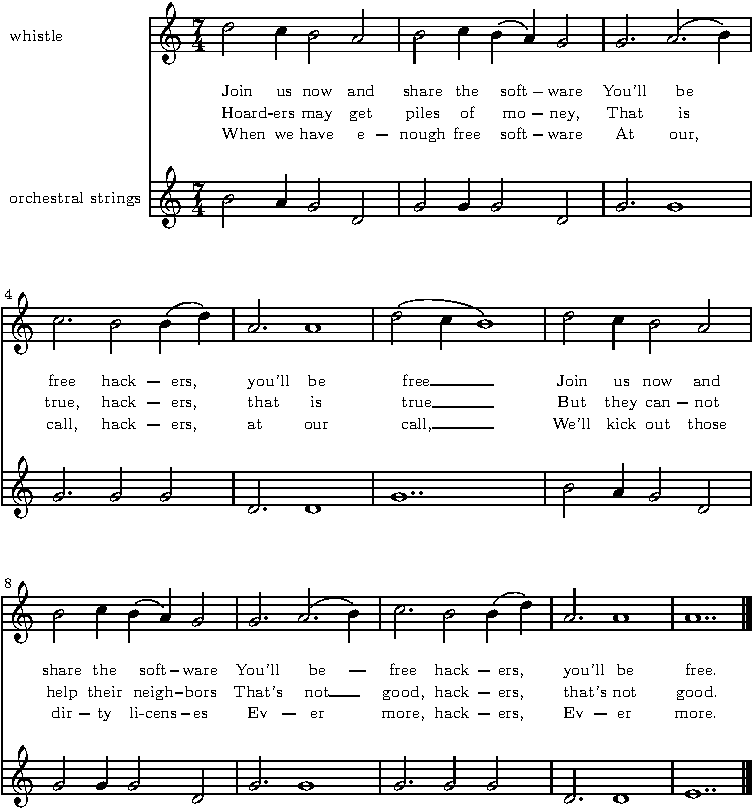
\includegraphics[scale=0.81, viewport=30 722 556 732]{free-song}

% \end{flushleft}
% \vskip 1cm

% \begin{quote}

% \footnotesize

% \begin{center}
% \noindent Copyright \copyright~1993 Richard Stallman. \\
% \noindent Se permite la copia y distribuci�n literal de esta partitura por
% cualquier medio, siempre que se mantenga esta nota.  
% \end{center}

% \smallskip

% \noindent Transcrito con GNU LilyPond por David Madore. \LaTeX eado y 
% convertido a la versi�n 2.2 de LilyPond para la edici�n de Traficantes de
% Sue�os por Miquel Vidal.

% \end{quote}

\normalsize

%% fin partitura %%


%   secci�n dos
\part{Copyright, copyleft, patentes}

\chapter[El derecho a leer]{El derecho a leer\protect\footnote{Escrito
originalmente en el n�mero de febrero de 1997 de la revista
\textit{Communications of the ACM} (Volumen 40, N�mero 2). La <<Nota del
Autor>> fue actualizada en 2002.}}

\begin{quote}

(De <<El camino a Tycho>>, una colecci�n de art�culos sobre los antecedentes de
la \textit{Revoluci�n Lunaria}, publicado en \textit{Luna City }en 2096.)

\end{quote}


Para Dan Halbert, el camino hacia Tycho comenz� en la universidad, cuando
Lissa Lenz le pidi� prestado su ordenador. El suyo se hab�a estropeado, y a
menos que pudiese usar otro suspender�a el proyecto de fin de trimestre. Ella
no se habr�a atrevido a ped�rselo a nadie, excepto a Dan.

Esto puso a Dan en un dilema. Ten�a que ayudarla, pero si le prestaba su
ordenador ella podr�a leer sus libros. Dejando a un lado el peligro de acabar
en la c�rcel durante muchos a�os por permitir a otra persona leer sus libros,
al principio la simple idea le sorprendi�. Como todo el mundo, hab�a aprendido
desde los a�os de colegio que compartir libros era malo, algo que s�lo un
pirata har�a.

Adem�s, era muy improbable que la SPA ---Software Protection Authority,
[Autoridad para la Protecci�n del Software]--- lo descubriese. En sus clases
de programaci�n, hab�a aprendido que cada libro ten�a un control de copyright
que informaba directamente a la oficina central de licencias de cu�ndo y d�nde
se estaba leyendo, y qui�n le�a ---utilizaban esta informaci�n para descubrir
a los piratas de la lectura, pero tambi�n para vender perfiles personales a
otros comercios. La pr�xima vez que su ordenador se conectase a la red, la
oficina central de licencias lo descubrir�a todo. �l, como propietario del
ordenador, recibir�a el castigo m�s duro por no tomar las medidas necesarias
para evitar el delito.

Por supuesto, podr�a ser que Lissa no quisiera leer sus libros. Probablemente
lo �nico que necesitaba del ordenador era redactar su proyecto. Pero Dan sab�a
que ella proven�a de una familia de clase media, que a duras penas se pod�a
permitir pagar la matr�cula y no digamos las tasas de lectura. Leer sus libros
pod�a ser la �nica forma por la que podr�a terminar la carrera. Comprend�a la
situaci�n; �l mismo hab�a pedido un pr�stamo para pagar por los art�culos de
investigaci�n que le�a ---el 10\% de ese dinero iba a parar a sus autores y
como Dan pretend�a hacer carrera en la Universidad, esperaba que sus art�culos
de investigaci�n, en caso de ser citados frecuentemente, le dar�an suficientes
beneficios como para pagar el cr�dito.

Con el paso del tiempo, Dan descubri� que hubo una �poca en que todo el mundo
pod�a acudir a una biblioteca y leer art�culos, incluso libros, sin tener que
pagar. Hab�a investigadores independientes que pod�an leer miles de p�ginas
sin necesidad de recurrir a becas de biblioteca. Pero desde los a�os noventa
del siglo anterior, las editoriales, tanto comerciales como no comerciales,
hab�an empezado a cobrar por el acceso a los art�culos. En 2047, las
bibliotecas con acceso p�blico a literatura acad�mica eran s�lo un vago
recuerdo.

Hab�a formas de saltarse los controles de la SPA y de la oficina central de
licencias. Pero tambi�n eran ilegales. Dan conoci� a un compa�ero de clase,
Frank Martucci, que consigui� una herramienta ilegal de depuraci�n y
la usaba para saltarse el control de \textit{copyright} de los libros. Pero se
lo cont� a demasiados amigos, y uno de ellos le denunci� a la SPA a cambio de
una recompensa ---era f�cil tentar a los estudiantes endeudados para
traicionar a sus amigos. En 2047, Frank estaba en la c�rcel, pero no por
pirateo, sino por tener un \textit{depurador}.

Dan averigu� m�s tarde que hubo un tiempo en que cualquiera pod�a
tener un depurador. Hab�a incluso depuradores gratuitos en
CD o disponibles libremente en la red. Pero los usuarios normales
empezaron a usarlos para saltarse los controles de \textit{copyright} y por
fin un juez dictamin� que �se se hab�a convertido en su principal uso
pr�ctico. Eso significaba que los depuradores eran ilegales y los
programadores que los crearon fueron a parar a la c�rcel.

Obviamente, los programadores a�n necesitan depuradores, pero en 2047
s�lo hab�a copias numeradas de los depuradores comerciales, y s�lo estaban
disponibles para los programadores oficialmente autorizados. El depurador que
Dan hab�a utilizado en sus clases de programaci�n estaba detr�s de un
cortafuegos para que s�lo pudiese utilizarse en los ejercicios de clase.

Tambi�n se pod�a saltar el control de \textit{copyright} instalando el kernel
de un sistema modificado. Dan descubri� que hacia el cambio de siglo hubo
kernels libres, incluso sistemas operativos completos. Pero ahora no s�lo eran
ilegales, como los depuradores. No se pod�a instalar sin saber la clave de
superusuario del ordenador y ni el FBI ni el servicio t�cnico de Microsoft la
revelar�an.

Dan lleg� a la conclusi�n de que simplemente no pod�a dejarle a Lissa su
ordenador. Pero no pod�a negarse a ayudarla, porque estaba enamorado de ella.
Cada oportunidad de hablar con ella era algo maravilloso. Y el hecho de que le
hubiese pedido ayuda a �l pod�a significar que ella sent�a lo mismo.

Dan resolvi� el dilema haciendo algo incluso m�s incre�ble, le dej� su
ordenador y le dio su clave. De esta forma, si Lissa le�a sus libros, la
oficina central de licencias pensar�a que era �l quien estaba leyendo. Segu�a
siendo un delito, pero la SPA no lo detectar�a autom�ticamente. S�lo podr�an
descubrirlo si Lissa le denunciaba.

Si la universidad descubriese que le hab�a dado su clave a Lissa, significar�a
la expulsi�n de ambos, independientemente del uso que hubiera hecho ella de su
clave. La pol�tica de la Universidad era que cualquier interferencia con sus
m�todos de control sobre el uso de los ordenadores era motivo de acci�n
disciplinaria. No importaba el da�o, el delito era el hecho de dificultar el
control. Se daba por supuesto que esto significaba que se estaba haciendo algo
prohibido, no necesitaban saber qu�.

En realidad, los estudiantes no eran expulsados, no directamente. En lugar de
eso, se les prohib�a el acceso a los ordenadores de la universidad, lo que
equival�a a suspender sus asignaturas.

Dan supo m�s tarde que ese tipo de pol�ticas en la Universidad comenz� durante
la d�cada de 1980, cuando los estudiantes empezaron a usar los ordenadores en
masa. Antes, las universidades ten�an una actitud diferente: s�lo se
penalizaban las actividades peligrosas, no las meramente sospechosas.

Lissa no denunci� a Dan a la SPA. Su decisi�n de ayudarla llev� a que se
casaran y tambi�n a que cuestionaran lo que les hab�an ense�ado cuando eran
ni�os sobre la pirater�a. Empezaron a leer sobre la historia del
\textit{copyright}, sobre la Uni�n Sovi�tica y sus restricciones sobre las
copias, e incluso sobre la constituci�n original de los Estados Unidos. Se
mudaron a Luna City, donde se encontraron con otros que intentaban librarse
del largo brazo de la SPA de la misma manera. Cuando el Levantamiento de Tycho
se produjo en 2062, el derecho universal a leer se convirti� en uno de sus
objetivos fundamentales.


\section{Nota del autor}

El derecho a leer es una batalla que se est� librando hoy en d�a. Aunque
nuestra forma de vida actual podr�a tardar cincuenta a�os en desaparecer, la
mayor�a de las leyes y de las pr�cticas descritas anteriormente ya han sido
propuestas, y muchas han entrado en vigor dentro y fuera de los Estados
Unidos. En EE.UU., el \textit{Digital Millenium Copyright Act} de 1998
estableci� la base legal para restringir la lectura y el pr�stamo de libros
informatizados ---as� como de otras clases de datos. La Uni�n Europea impuso
restricciones similares con su directiva sobre \textit{copyright} de 2001.

Hasta hace poco hab�a una excepci�n, la idea de que el FBI y Microsoft
guardaran las claves de administraci�n de los ordenadores personales y no las
dejasen tener no fue propuesta hasta 2002: se le denomina <<Inform�tica de
Confianza>> o <<Palladium>>. 

Cada vez estamos m�s cerca de este punto. En 2001 el Senador Hollings,
financiado por la Disney, propuso un proyecto de ley llamado SSSCA ---ahora
rebautizado como la CBDTPA--- que podr�a requerir que todos los nuevos
ordenadores tuviesen aplicaciones obligatorias de restricci�n de copia que el
usuario no podr�a puentear

En 2001 los Estados Unidos, empezaron a intentar utilizar la llamada �rea de
Libre Comercio de las Am�ricas (ALCA) para imponer las mismas normas en todos
los pa�ses del hemisferio occidental. El ALCA es uno de los denominados
tratados de <<libre comercio>>, dirigido actualmente a otorgar mayor poder a las
empresas sobre los gobiernos democr�ticos; imponiendo leyes como la DMCA que
son t�picas de su esp�ritu. La Electronic Frontier Foundation anima a la gente
a que explique a sus gobiernos por que deber�an oponerse a esos planes.

La SPA que en realidad corresponde a la Software Publisher's Association, ha
sido reemplazada en su papel por la BSA o Business Software Aliance. La BSA no
es un cuerpo de polic�a oficial. Act�a como tal extraoficialmente. Usa m�todos
de delaci�n que tienen reminiscencias en la antigua Uni�n Sovi�tica. Anima a
la gente a informar sobre sus compa�eros de trabajo y sus amigos. Promovi� una
campa�a de terror en Argentina, durante 2001, amenazando con la c�rcel a todo
aquel que compartiese software.

Cuando este art�culo fue escrito, la SPA amenazaba a los peque�os
proveedores de Internet para que le permitiesen controlar a todos sus
usuarios. Muchos ISP cedieron ante las amenazas, ya que no pod�an permitirse
recurrir a la v�a judicial. Al menos un ISP, Community ConneXion, en Oakland
(California), se neg� a ceder a las presiones y ha sido demandado.
Aparentemente, la SPA retir� la demanda hace poco, pero no hay duda de que
continuar�n su campa�a por otros medios.

Las pol�ticas universitarias de seguridad descritas arriba no son imaginarias.
Por ejemplo, el ordenador de una universidad de la zona de Chicago despliega
el siguiente mensaje al entrar en el sistema:

\begin{quote}

\small

<<Este sistema s�lo puede ser utilizado por usuarios autorizados. Cualquier
persona que utilice este sistema sin autorizaci�n o fuera de los l�mites
autorizados ser� vigilado por el personal administrador del sistema. Durante
el control de usuarios que realicen actividades no autorizadas o durante el
mantenimiento del sistema, las actividades de los usuarios autorizados podr�n
ser supervisadas. Cualquiera que utilice este sistema acepta expresamente este
control y deber� saber que, en caso de que dicho control revelara posibles
indicios de actividades ilegales o de violaci�n de las normas de la
universidad, el personal de mantenimiento del sistema podr� proporcionar estas
pruebas a las autoridades de la Universidad y/o a las fuerzas de seguridad.>>

\end{quote}

\normalsize

Esta es una interesante interpretaci�n de la Cuarta Enmienda: obligar a los
usuarios a renunciar por adelantado a los derechos contemplados en ella.



\section{Referencias}

\begin{itemize}

\item El \textit{White Paper} del Gobierno\textit{: Information Infraestructure Task
Force, Intellectual Property and the National Information Infraestructure: The
Report of the Working Group on Intellectual Property Rights} (1995).

\item \textit{An explanation of the White Paper: The Copyright Grab}, Pamela
Samuelson, Wired, enero de 1996.

\item \textit{Sold Out}, James Boyle, The New York Times, 31 de marzo de 1996.

\item \textit{Public Data or Private Data}, The Washington Post, 4 de noviembre de
1996.

\item \textit{Union for the Public Domain}, una nueva organizaci�n que pretende
resistirse y frenar la desmedida generalizaci�n de la propiedad intelectual.

\end{itemize}

\chapter[Malinterpretar el copyright: una sucesi�n de errores]{Malinterpretar el copyright: una sucesi�n de errores\protect\footnote{Publicado originalmente en este libro.}}

Algo extra�o y peligroso est� sucediendo en la legislaci�n sobre el copyright.
Seg�n la Constituci�n de los Estados Unidos, el copyright existe para
beneficiar a los usuarios ---los que leen libros, escuchan m�sica o utilizan
software---, no para beneficiar a los editores o los autores. A�n cuando la
gente tiende cada vez m�s a rechazar y desobedecer las limitaciones del
copyright que le vienen impuestas <<por su propio beneficio>>, el gobierno de
los Estados Unidos est� a�adiendo m�s restricciones y trata de asustar al
p�blico con nuevas y r�gidas penas con el fin de conducirlo a la sumisi�n.
�C�mo lleg� la pol�tica de copyright\textit{ }a ser diametralmente opuesta a
su prop�sito establecido? �C�mo podemos volver a alinearla con ese prop�sito?
Para comprenderlo, debemos empezar por considerar la ra�z de la legislaci�n
estadounidense sobre copyright: la Constituci�n de los Estados Unidos.


\section{El copyright en la Constituci�n de los Estados Unidos}

Cuando se dise�� la Constituci�n de los Estados Unidos, se propuso la idea de
que se concediera a los autores un monopolio sobre el copyright ---la
propuesta fue rechazada. Los fundadores de nuestro pa�s adoptaron un supuesto
diferente: que el copyright no es un derecho natural de los autores, sino una
concesi�n artificial que se les hace en nombre del progreso. La Constituci�n
concede carta legal al sistema de copyright con este p�rrafo (Art�culo I,
Secci�n 8):

\begin{quote}

\small

[El Congreso tendr� el poder] de promover el progreso de la ciencia y las
artes provechosas, asegurando por tiempo limitado a los inventores y autores
el exclusivo derecho sobre sus respectivos descubrimientos y escritos.

\end{quote}
    
\normalsize

El Tribunal Supremo ha afirmado repetidas veces que promover el progreso
significa un beneficio para los usuarios de las obras sujetas a copyright. Por
ejemplo, en el caso de la Fox Film contra  Doyal, el tribunal dict�:

\begin{quote}

\small

El exclusivo inter�s de los Estados Unidos y el objeto primordial de conceder
el monopolio [del copyright] reside en los beneficios generales obtenidos por
el p�blico a partir del trabajo de los autores.

\end{quote}
    
\normalsize

Esta decisi�n fundamental explica por qu� el copyright no es
\textit{obligatorio} seg�n la Constituci�n y es s�lo algo \textit{permitido}
como una opci�n ---tambi�n explica por qu� se supone que su duraci�n alcanza
un <<tiempo limitado>>. Si el copyright fuera un derecho natural, algo que los
autores tienen en tanto depositarios de ese derecho, nada justificar�a la
extinci�n de este derecho pasado un determinado periodo de tiempo, como si los
hogares de cada uno pasaran a ser propiedad p�blica cierto tiempo despu�s de
su construcci�n.


\section[El <<contrato>> del copyright]{El <<contrato\protect\footnote{N�tese
que el termino ingl\'{e}s \textit{bargain} puede referirse tanto a un trato
como a un chollo.  [\textit{N. del E.}]} de copyright>>}

El sistema de \textit{copyright} funciona mediante la concesi�n de privilegios
y por lo tanto de beneficios, a los editores y a los autores, pero no lo hace
en su provecho. M�s bien lo hace para modificar su comportamiento: proporciona
un incentivo a los autores para escribir y editar m�s. En la pr�ctica, el
gobierno emplea los derechos naturales del p�blico, en nombre del p�blico,
como parte de un trato para ofrecerle un mayor n�mero de obras editadas. Los
expertos en derecho llaman a este concepto el <<contrato de copyright>>; como la
adquisici�n estatal de una autopista o un avi�n usando el dinero de los
contribuyentes, excepto que en este caso el gobierno gasta nuestra libertad en
lugar de nuestro dinero.   

Pero �tal y como existe en la actualidad, el contrato supone un buen trato
para el p�blico? Son posibles muchos contratos alternativos; �cu�l es el
mejor? Cualquier medida en relaci�n a la pol�tica de copyright es parte de
esta cuesti�n. Si malinterpretamos la naturaleza de la cuesti�n,  tenderemos a
tomar medidas de forma err�nea. 

La Constituci�n permite que se concedan derechos de copyright a los autores.
En la pr�ctica, normalmente los autores se los ceden a los editores; son los
editores, y no los autores, quienes suelen ejercer los derechos y quienes se
quedan con la mayor�a de los beneficios, aunque los autores consigan una
peque�a porci�n. Por eso los editores son los que con frecuencia presionan m�s
para aumentar los poderes del copyright. Para reflejar mejor la realidad del
copyright en lugar del mito, este art�culo se refiere a los editores antes que
a los autores como sujetos de los derechos del copyright.  Tambi�n se refiere
a los usuarios de las obras protegidas por el copyright\textit{ }como
<<lectores>>, a�n cuando este uso no siempre signifique su lectura, en la medida
en que el t�rmino <<usuario>> resulta lejano y abstracto. 


\section{El primer error: <<equilibrar la balanza>>}

El contrato de copyright\textit{ }pone al p�blico en primer t�rmino: el
beneficio para el p�blico lector es un fin en s� mismo; los beneficios para
los editores ---si es que se dan--- son s�lo medios para conseguir ese fin. En
principio, los intereses de los lectores y los de los editores son
cualitativamente desiguales. El primer paso al malinterpretar el prop�sito del
copyright es elevar a los editores al mismo nivel de importancia que a los
lectores.

Se ha dicho con frecuencia que la legislaci�n estadounidense de copyright se
propone equilibrar la balanza entre los intereses de los editores y de los
lectores. Los que citan esta interpretaci�n la presentan como una
reformulaci�n del punto de partida establecido en la Constituci�n; en otras
palabras, se la supone equivalente al contrato de copyright.

Pero las dos interpretaciones est�n lejos de ser equivalentes; son
conceptualmente distintas y sus implicaciones son diferentes. La idea de la
balanza asume que los intereses de los editores y de los lectores difieren en
importancia de forma s�lo cuantitativa, en <<cu�nto al peso>> que debemos darles
y en qu� situaciones se deben aplicar. El concepto de <<la persona que guarda
las apuestas>> se suele usar para enmarcar la cuesti�n de este modo; supone que
al tomar una decisi�n todos los intereses son igual de importantes. Este
enfoque rechaza la distinci�n cualitativa entre los intereses de los lectores
y de los editores que est� en la base de la mediaci�n gubernamental en el
contrato de copyright.    

Las consecuencias de esta alteraci�n tienen un largo alcance, porque la fuerte
protecci�n que el p�blico recibe con el contrato del copyright ---a idea de
que los privilegios del copyright s�lo pueden justificarse en nombre de los
lectores y nunca en el nombre de los editores--- queda eliminada por esta
interpretaci�n de tipo <<balanza>>. Dado que el inter�s de los editores es
considerado como un fin en s� mismo, se puede justificar los privilegios del
copyright; en otras palabras, el concepto de <<balanza>> dicta que los
privilegios pueden justificarse en nombre de cualquiera que no sea el p�blico.

En la pr�ctica, la consecuencia del concepto de <<balanza>> es que
invierte el peso de las justificaciones en lo que respecta a la legislaci�n de
copyright. El contrato de copyright coloca el peso en los editores para
convencer a los lectores de que cedan ciertas libertades.  El concepto de
balanza pr�cticamente invierte este peso, porque en general no hay duda de que
los editores se benefician de privilegios adicionales. De modo que, si no se
prueba que el da�o causado a los lectores es lo bastante grande como para
<<equilibrar>> esos beneficios, se nos lleva a la conclusi�n de que los editores
tienen derecho a casi cualquier privilegio que reclamen. 

Dado que la idea de <<equilibrar la balanza>> entre editores y lectores niega a
los lectores la primac�a a la que tienen derecho, debemos rechazarla.  


\section{�Qu� se contraequilibra?}

Cuando el gobierno compra algo para el p�blico, act�a en su nombre; su
responsabilidad es obtener el mejor trato posible ---mejor para el p�blico, no
para la otra parte del acuerdo. 

Por ejemplo, cuando firma contratos con las constructoras para hacer
autopistas, el gobierno pretende gastar lo menor parte posible del erario
p�blico. Las agencias gubernamentales usan el sistema de concursos para forzar
los precios a la baja. 

En la pr�ctica, el precio no puede ser igual a cero, porque los contratistas
no pujar�n tan bajo. Aunque no tengan derecho a consideraciones especiales,
tienen los derechos ciudadanos corrientes en una sociedad libre, incluyendo el
derecho a rechazar contratos no ventajosos; incluso la oferta m�s baja ser�
suficiente para que alg�n contratista gane dinero. Luego ciertamente existe
alg�n tipo de equilibrio. Pero no se trata de un  equilibrio deliberado entre
dos intereses que reclaman un trato especial. Es un equilibrio entre el bien
p�blico y las fuerzas del mercado. El gobierno trata de obtener para los
contribuyentes automovilistas el mejor trato que puedan conseguir en el
contexto de una sociedad libre y de un mercado libre.

En el contrato de copyright, el gobierno emplea nuestra libertad en lugar de
nuestro dinero. La libertad es m�s valiosa que el dinero, as� que la
responsabilidad del gobierno en el empleo sabio y austero de nuestra libertad
es incluso mayor que su responsabilidad en el uso de nuestro dinero. Los
gobiernos jam�s deben poner los intereses de los editores a la par que la
libertad del p�blico. 


\section{Mejor concesi�n que <<equilibrio>>}   

La idea de equilibrar los intereses de los lectores con los intereses de los
editores es la forma m�s err�nea de juzgar la pol�tica de copyright, pero
ciertamente hay dos intereses que sopesar: dos intereses \textit{de los
lectores. }Los lectores est�n interesados en su propia libertad de consumir
obras publicadas; y seg�n las circunstancias, tambi�n estar�n interesados en
animar la publicaci�n mediante alg�n tipo de incentivos.

La palabra <<equilibrio>>, en las discusiones sobre copyright, ha quedado como
una abreviatura de la idea de <<equilibrar la balanza>> entre lectores y
editores. Por lo tanto, usar la palabra <<equilibrio>> a prop�sito de los dos
intereses de los lectores ser�a confuso ---necesitamos otro t�rmino.

En general, cuando un sujeto tiene dos objetivos que parcialmente entran en
conflicto, y no puede realizar ambos por completo, llamamos a esto una
concesi�n. Por lo tanto, mejor que hablar de <<equilibrar la balanza>> entre las
partes, deber�amos hablar de <<encontrar la concesi�n apropiada de libertad que
considere tanto su p�rdida necesaria como su conservaci�n>>.


\section{El segundo error: maximizar la producci�n}

El segundo fallo de la pol�tica de copyright consiste en adoptar el objetivo
de maximizar ---no simplemente aumentar--- la cantidad de obras publicadas. El
concepto err�neo de <<equilibrar la balanza>> alzaba a los editores al nivel de
los lectores; este segundo error los sit�a muy por encima de ellos. 

Cuando adquirimos algo, por lo general no compramos toda la cantidad
disponible ni tampoco el modelo m�s caro. En su lugar conservamos fondos para
otras adquisiciones, comprando s�lo lo que necesitamos de un bien particular o
escogiendo un modelo est�ndar antes que el de m�s alta calidad. El principio
de los rendimientos decrecientes ense�a que gastar todo nuestro dinero en un
bien particular tiende a ser una ineficiente asignaci�n de recursos; por lo
general preferimos guardar algo de dinero para otro uso. 

La ley de rendimientos decrecientes se ajusta al copyright tanto como a
cualquier otra adquisici�n. Las primeras libertades que deber�amos ceder son
aquellas que menos echamos de menos, al tiempo que damos el mayor respaldo a
la publicaci�n. Seg�n cedemos libertades adicionales que se acercan m�s a lo
que nos importa, encontramos que cada cesi�n supone un mayor sacrificio que la
anterior, mientras que aporta un menor incremento a la actividad literaria.
Antes de que el incremento sea igual a cero, bien podr�amos decir que su
creciente precio no merece la pena; entonces fijar�amos un contrato cuyo
resultado general es incrementar la cantidad de lo publicado, pero no hasta su
�ltimo extremo posible. 

Aceptar el objetivo de maximizar la publicaci�n supone rechazar de entrada
todos estos contratos m�s ventajosos ---este objetivo dispone que el p�blico
debe ceder casi toda su libertad de usar obras publicadas, a cambio de s�lo
unas pocas publicaciones m�s.


\section{La ret�rica de la maximizaci�n}

En la pr�ctica, el objetivo de maximizar la producci�n sin que importe su
coste para la libertad se sustenta en la extendida ret�rica que asegura que la
copia p�blica es ilegal, ileg�tima, injusta e intr�nsecamente err�nea. Por
ejemplo, los editores llaman <<piratas>> a la gente que copia, t�rmino
difamatorio pensado para equiparar el intercambio de informaci�n con tu vecina
con el abordaje a un barco. (Este t�rmino difamatorio fue anteriormente usado
por los autores para describir a los editores que encontraron formas legales
de publicar ediciones no autorizadas; su uso moderno por parte de los editores
es casi su reverso). Esta ret�rica rechaza directamente la base constitucional
del copyright, pero se presenta a s� misma como representante de la
incontestada tradici�n del sistema legal americano.

La ret�rica del <<pirata>> es aceptada frecuentemente en la misma medida en que
ciega a los medios de comunicaci�n, de tal modo que poca gente se da cuenta de
su extremismo. Resulta efectiva porque si la copia por parte del p�blico es
fundamentalmente ileg�tima, nunca podremos oponernos a los editores que exigen
nuestra renuncia a la libertad de copiar. En otras palabras, cuando se reta al
p�blico a demostrar por qu� los editores no deben recibir m�s poder, la raz�n
m�s importante de todas ---<<queremos copiar>>--- es descalificada de entrada.

Esto no deja lugar para contestar el creciente poder del copyright sin entrar
en cuestiones secundarias. Por lo tanto la oposici�n actual a un mayor poder
del copyright alega exclusivamente cuestiones secundarias y nunca se atreve a
alegar la libertad de distribuir copias como un valor p�blico leg�timo.

En concreto, el objetivo de la maximizaci�n capacita los editores para
argumentar que <<cierta pr�ctica est� reduciendo nuestras ventas ---o pensamos
que podr�a reducirlas---, as� que suponemos que reduce las publicaciones en
una cantidad desconocida, y que por lo tanto debe ser prohibida>>. Se nos lleva
a la espantosa conclusi�n de que el bien p�blico se mide por las ventas de los
editores: lo que es bueno para General Media es bueno para EE.UU.  


\section{El tercer error: maximizar el poder de los editores}

Una vez que los editores han obtenido el consentimiento para el objetivo
estrat�gico de maximizar la producci�n de publicaciones a cualquier coste, su
pr�ximo paso es probar que esto obliga a otorgarles los mayores poderes
posibles ---haciendo que el copyright cubra cualquier uso imaginable de una
obra o aplicando cualquier otro instrumento legal como las licencias <<de sobre
cerrado>> para conseguir un efecto equivalente. Este objetivo, que impone la
abolici�n del <<uso razonable>>  y el <<derecho sobre la primera
venta>>, est� siendo objeto de presi�n en todos los niveles
de gobierno imaginables, desde los estados de los EE.UU. hasta los organismos
internacionales. 

Esta medida es err�neo porque las reglas estrictas de copyright obstruyen la
creaci�n de nuevas obras �tiles. Por ejemplo, Shakespeare tom� prestados los
argumentos de algunas de sus obras teatrales de otras obras publicadas unas
pocas d�cadas antes, de modo que de haber estado en funcionamiento la actual
legislaci�n de copyright, sus obras habr�an sido ilegales. 

Incluso si dese�ramos el mayor grado posible de publicaci�n, sin que importara
el costo para el p�blico, maximizar el poder de los editores es una forma
err�nea de conseguirlo. Como medio de promover el progreso, es
autodestructivo.


\section{Resultados de los tres errores}

La tendencia actual en la legislaci�n de copyright es proporcionar a los
editores poderes m�s amplios por periodos de tiempo cada vez m�s largos. La
base conceptual del copyright, en la medida en que resulta distorsionada por
esta secuencia de errores, rara vez ofrece una base para decir no. Los
legisladores defienden de boquilla la idea de que el copyright sirve al
p�blico, mientras que en realidad dan a los editores cualquier cosa que pidan.

Por ejemplo, esto es lo que dijo el senador Hatch al introducir la S. 483, una
ley dictada en 1995 que incrementa la duraci�n del copyright 20 a�os m�s: 

\begin{quote}

\small

Creo que hemos llegado al punto de preguntarnos si la duraci�n actual del
copyright protege adecuadamente los intereses de los autores, y la cuesti�n
correlativa de si el tiempo de protecci�n sigue proporcionando suficientes
incentivos para la creaci�n de nuevas obras.

\end{quote}

\normalsize

Esta ley extendi� el copyright para obras publicadas y escritas desde
1920. Este cambio supuso una ganga para los editores, sin beneficio posible
para el p�blico, dado que ahora no hay modo de aumentar retroactivamente la
cantidad de libros publicados entonces. Sin embargo cost�
al p�blico una libertad hoy muy significativa ---la libertad de redistribuir
libros de esa �poca.

La ley tambi�n extendi� el copyright de las obras que a�n no han sido
escritas. Para trabajos de encargo, el copyright durar�a 95
a�os en lugar de los 75 a�os que dura hoy. Te�ricamente esto aumentar�a los
incentivos para escribir nuevos libros, pero cualquier editor que diga
necesitar este incentivo extra deber�a apoyar esta pretensi�n con hojas de
balance proyectadas hasta el a�o 2075.

No hace falta decir que el Congreso no cuestion� los argumentos de los
editores: en 1998 fue promulgada la ley que extend�a la duraci�n del
copyright. Fue conocida como la <<ley Sonny Bono para la extensi�n de la
duraci�n del copyright>>, as� llamada por uno de sus promotores, que hab�a
muerto ese a�o. Su viuda, que cubri� el resto de su trabajo, hizo esta 
declaraci�n:

\begin{quote}

\small

En realidad, Sonny quer�a que el copyright durase para siempre. Mis abogados
me han informado de que tal cambio violar�a la Constituci�n. Os invito a todos
vosotros a trabajar conmigo para reforzar nuestras leyes de copyright de todos
los modos a nuestro alcance. Como sab�is, tambi�n est� la propuesta de Jack
Valenti para que dure para siempre menos un d�a. Quiz� el comit� pueda tratar
este asunto el pr�ximo Congreso. 

\end{quote}

\normalsize

El Tribunal Supremo ha admitido un pleito que busca derogar esta ley con el
fundamento de que la retroactividad no sirve al objetivo constitucional de
promover el progreso. 

Otra ley, aprobada en 1996, convirti� en una fechor�a hacer determinadas
copias de cualquier obra publicada, incluso si vas a repartirlas entre amigos
simplemente por amabilidad. Antes esto en absoluto era un crimen en los EE.UU.

Una ley todav�a peor, la \textit{Digital Millenium Copyright Act} (DMCA) fue
dise�ada para traer de vuelta la protecci�n frente a las copias ---que los
usuarios de ordenadores detestan--- convirtiendo en un crimen cualquier
infracci�n de esta protecci�n, o incluso publicar informaci�n sobre c�mo
quebrar esta protecci�n. Esta ley deber�a de llamarse <<ley para la dominaci�n
por parte de las empresas mass-medi�ticas>> porque ofrece efectivamente a los
editores la oportunidad de escribir su propia ley de copyright. Dicta que
pueden imponer cualquier tipo de restricciones en el uso de una obra, y estas
restricciones tienen el rango de ley siempre que la obra contenga alg�n tipo
de cifrado o gestor de licencias que haga efectivo su
cumplimiento. 

Uno de los argumentos ofrecidos por esta ley era que implementar�a un reciente
tratado para aumentar la extensi�n del copyright. Este tratado fue promulgado
por la Organizaci�n Mundial de la Propiedad Intelectual (OMPI), organizaci�n
dominada por  los propietarios de los derechos de autor y de patentes, con la
ayuda del gobierno de Clinton; dado que el tratado s�lo aumenta la extensi�n
del copyright, es dudoso que sirva al inter�s p�blico en ning�n pa�s. En
cualquier caso, la ley fue mucho m�s lejos de lo que el tratado demandaba.

Las bibliotecas fueron una fuente clave de oposici�n a esta ley, especialmente
en los aspectos que coartan las formas de copia que se consideran de <<uso
razonable>>. �C�mo respondieron los editores? El antes
diputado Pat Schroeder, ahora miembro del grupo de presi�n a favor de la
Asociaci�n de Editores Americanos, dijo que los editores <<no podr�an vivir con
lo que (las bibliotecas) est�n pidiendo>>. Dado que las bibliotecas s�lo
estaban pidiendo que se mantuviera parte del \textit{statu quo}, uno podr�a
contestar preguntando c�mo hab�an sobrevivido los editores hasta entonces. 

El congresista Barney Frank, durante una reuni�n conmigo y otros opositores a
esta ley, demostr� cu�nto se ha menospreciado la visi�n que la Constituci�n de
los EE.UU. tiene sobre el copyright. Dijo que se necesitan urgentemente
nuevos poderes respaldados por nuevas penas, puesto que <<la industria del cine
est� preocupada>>, as� como la <<industria de la m�sica>> y otras <<industrias>>.
Yo le pregunt�, <<�pero todo esto es para el inter�s general?>> Su respuesta
vino a decir: <<�Por qu� me hablas del inter�s general? �La gente creativa no
tiene que abandonar sus derechos en favor del inter�s general!>> La <<industria>>
ha sido identificada con <<la gente creativa>> a la que contrata, el copyright
ha sido tratado como su privilegio y la Constituci�n ha sido puesta patas
arriba.

La DMCA fue publicada en 1998. Esta ley dice que el uso razonable sigue siendo
leg�timo, pero permite a los editores prohibir todo el software o el hardware
con el que podr�as ponerlo en pr�ctica. De hecho, el uso razonable est�
prohibido. 

Bas�ndose en esta ley, la industria del cine ha impuesto la censura al
software libre por leer y reproducir DVDs, e incluso a la informaci�n sobre
c�mo leerlos. En abril de 2001 el profesor Edward Felten, de la universidad de
Princeton, fue intimidado bajo amenaza de una demanda judicial por parte de la
Asociaci�n de la Industria Americana de Grabaci�n, con el objetivo de que
retirara un art�culo cient�fico en el que expon�a lo que hab�a aprendido
acerca de un sistema piloto de encriptaci�n que restring�a el acceso a las
grabaciones musicales. 

Tambi�n estamos empezando a ver libros electr�nicos que retiran a los lectores
muchas de sus libertades tradicionales ---por ejemplo, la libertad de prestar
un libro a un amigo, de venderlo a una tienda de libros usados, de tomarlo
prestado de una biblioteca, de comprarlo sin darle tu nombre a una base de
datos empresarial, incluso la libertad de leerlo dos veces. Los libros
electr�nicos codificados restringen por lo general este tipo de actividades
---s�lo puedes leerlos con un software especial secreto dise�ado para limitar
tus libertades.

Nunca comprar� uno de esos libros electr�nicos, cifrados y restrictivos, y
espero que t� tambi�n los rechaces. �Si un libro electr�nico no te da las
mismas libertades que un libro tradicional de papel, no lo aceptes!

Cualquiera que lance por su cuenta software que pueda leer libros electr�nicos
restrictivos se arriesga a ser acusado. Un programador ruso, Dmitry Sklyarov,
fue arrestado en 2001 mientras visitaba EE.UU. para dar en una conferencia,
porque hab�a escrito un programa de esas caracter�sticas en Rusia, donde
hacerlo era legal. Ahora Rusia tambi�n est� preparando una ley para prohibirlo
y la Uni�n Europea ha adoptado una similar recientemente. 

Los libros electr�nicos para el mercado de masas han resultado hasta ahora un
fracaso comercial, pero no porque los lectores elijan defender su libertad; no
eran atractivos por otras razones, como el hecho de que los monitores de los
ordenadores no son soportes c�modos para la lectura. No podemos confiar en
esta feliz casualidad para protegernos a largo plazo; el pr�ximo intento para
promocionar los libros electr�nicos usar� <<papel electr�nico>> ---objetos
parecidos a libros dentro de los cuales se puede descargar un libro
electr�nico codificado y restringido. Si este soporte parecido al papel
demuestra ser m�s atractivo que los actuales monitores, tendremos que defender
nuestra libertad para conservarla. Mientras tanto, los libros electr�nicos
est�n penetrando nichos de mercado: la NYU y otras escuelas de odontolog�a
obligan a sus estudiantes a comprar sus libros de texto con formato de libros
electr�nicos restrictivos. 

Las empresas medi�ticas no est�n satisfechas todav�a. En 2001, el senador
Hollings ---financiado por la Disney--- propuso una ley llamada <<ley para los
est�ndares de los sistemas de seguridad y de las certificaciones>>,
\footnote{Luego rebautizada con el nombre impronunciable de LPCBATD, para la
cual <<consume, pero no intentes programar nada>> es un buen recordatorio; pero
las siglas significan realmente  Ley de Promoci�n del Consumo de Banda Ancha y
Televisi�n Digital.} que obligar�a a que todos los ordenadores ---y otros
dispositivos de grabaci�n y reproducci�n digital--- tuvieran sistemas
restrictivos de copia por mandato del gobierno. Ese es su objetivo final, pero
el primer punto de su agenda es prohibir cualquier equipo que pueda sintonizar
HDTV digital a no ser que est� dise�ado para que al p�blico le sea imposible
<<entrometerse>> ---por ejemplo, modificarlo para sus propios fines. Dado que
el software libre es software que los usuarios pueden modificar, aqu� nos
enfrentamos por primera vez con una propuesta de ley que proh�be
expl�citamente el software libre para un trabajo determinado. Seguramente, le
seguir� la prohibici�n de otros trabajos. Si el FCC adopta esta regla, el
software libre hoy existente, como GNU Radio, ser�a censurado. 

La acci�n pol�tica es necesaria para bloquear estas leyes y reglamentos.
\footnote{Si quieres ayudar, te recomiendo los sitios web
\url{digitalspeech.org} y \url{www.eff.org}.}

\section{Encontrar el contrato adecuado}

�Cu�l es la manera adecuada de decidir la pol�tica de copyright? Si el
copyright es un contrato hecho en nombre del p�blico, deber�a servir ante todo
al inter�s p�blico. El deber del gobierno al vender la libertad del p�blico es
vender s�lo lo que debe y venderlo tan caro como sea posible. Como m�nimo,
deber�amos recortar, en la medida de lo posible, el alcance del copyright
mientras podamos un nivel comparable de publicaci�n. 

Dado que no podemos encontrar este precio m�nimo en t�rminos de libertad a
trav�s de un concurso p�blico como se hace con los proyectos de construcci�n,
�qu� podemos hacer?

Un m�todo posible es reducir los privilegios del copyright por etapas y
observar los resultados. Observando si hay disminuciones apreciables en el
volumen de publicaci�n, aprenderemos que extensi�n del copyright\textit{ }es
realmente necesaria para llevar a cabo los prop�sitos del p�blico. Esto se
debe valorar por medio de la observaci�n pr�ctica, no por lo que los editores
digan que ocurrir�, ya que tienen todos los motivos para hacer predicciones
exageradas de perdidas si sus poderes se ven reducidos de alg�n modo.

 La pol�tica de copyright tiene varias dimensiones independientes que
 pueden ajustarse de forma separada. Despu�s de encontrar el m�nimo necesario
 para una vertiente de esta pol�tica, todav�a ser�a posible reducir otras
 dimensiones del copyright a la vez que se mantiene el nivel de publicaci�n
 deseado. 

Una dimensi�n importante del copyright es su duraci�n, que ahora se encuentra
en torno a un siglo de media. Reducir el monopolio sobre la copia a diez a�os,
desde la fecha en que una obra es publicada, ser�a un buen primer paso. Otro
aspecto del copyright, que cubre la realizaci�n de obras derivadas, podr�a
extenderse por m�s tiempo. 

�Por qu� contar desde la fecha de publicaci�n? Por que el copyright de las
obras no publicadas no limita directamente la libertad los lectores; que
tengamos libertad para copiar una obra es una cuesti�n in�til cuando aun no
tenemos una  copia. As� que dar a los autores m�s tiempo para publicar un
trabajo no hace ning�n da�o. Los autores ---que por lo general s� poseen el
\textit{copyright} antes de publicar--- rara vez elegir�n retrasar la
publicaci�n s�lo para alejar el fin del plazo del copyright. 

�Por qu� diez a�os? Porque  esta es una propuesta segura; podemos confiar en
el terreno pr�ctico que esta reducci�n tendr�, hoy en d�a, poco impacto en la
viabilidad general de la edici�n. En muchos medios y g�neros, las obras de
�xito son muy rentables unos pocos a�os, y normalmente incluso las obras de
�xito ya no se editan pasados los diez a�os. Incluso para las obras de
referencia, cuya vida �til puede ser de muchas d�cadas, el copyright de diez
a�os deber�a de bastar: las ediciones actualizadas se lanzan con regularidad y
muchos lectores comprar�n la �ltima versi�n con copyright antes que copiar una
versi�n de dominio p�blico con diez a�os de antig�edad. 

Diez a�os todav�a puede ser m�s tiempo del necesario; una vez que las cosas se
estabilicen, podremos probar mayores reducciones para ajustar el sistema. En
una mesa redonda sobre copyright durante una convenci�n literaria, en la que
yo propuse el plazo de diez a�os, un famoso escritor de fantas�a que se
sentaba junto a m� protest� vehementemente, diciendo que cualquier cosa que
sobrepasara los cinco a�os era intolerable. 

Pero no tenemos por qu� aplicar el mismo lapso de tiempo para todas las obras.
Mantener la uniformidad extrema de las pol�ticas de copyright no es crucial
para el inter�s p�blico y la legislaci�n de copyright ya incluye muchas
excepciones para medios y usos espec�ficos. Ser�a est�pido pagar por cada
proyecto de autopista al precio de los proyectos m�s dif�ciles y en las
regiones m�s caras del pa�s; es igualmente est�pido <<pagar>> por todo tipo de
arte el precio m�s alto, en t�rminos de libertad, que consideramos necesario
para un caso determinado.  

As�, quiz�s las novelas, los diccionarios, los programas inform�ticos, las
canciones, las sinfon�as y las pel�culas deber�an tener un copyright con
distintas duraciones, de modo que podamos reducir la duraci�n en cada tipo de
obra a lo que sea necesario para ese tipo de obras se publiquen. Quiz� las
pel�culas con duraci�n mayor de una hora podr�an tener un copyright de 20
a�os, debido a los costes de producci�n. En mi propio campo, la programaci�n
inform�tica, tres a�os deber�an bastar, dado que los ciclos de un producto son
incluso m�s cortos.

Otra dimensi�n de la pol�tica de copyright es la magnitud del uso razonable:
algunas formas legalmente permitidas de reproducci�n de un trabajo, total o
parcialmente, a�n cuando �ste est� protegido por el copyright. El primer paso
natural para reducir este aspecto del copyright es permitir la copia privada
sin �nimo de lucro, ocasional y en peque�a cantidad, para su distribuci�n
entre individuos. Esto eliminar�a la intrusi�n de la polic�a del copyright en
la vida privada de la gente, pero probablemente tendr�a poco efecto en las
ventas de las obras publicadas. (Podr�a ser necesario tomar otras medidas
legales para asegurar que las licencias de uso de <<sobre cerrado>> no sean
usadas para sustituir al copyright y restringir este tipo de copia.) La
experiencia de Napster muestra que tambi�n deber�amos permitir al p�blico
general la redistribuci�n textual y no comercial ---cuando tanta gente entre
el p�blico quiere copiar y compartir, y lo encuentra tan �til, s�lo
conseguir�n detenerlo medidas draconianas; el p�blico tiene derecho a obtener
lo que quiere. 

Para las novelas, y en general para las obras que se utilizan como
entretenimiento, la redistribuci�n textual no comercial podr�a ser una
libertad suficiente para los lectores. Los programas inform�ticos, al ser
usados para fines funcionales ---para trabajar---, exigen libertades
adicionales, incluyendo la libertad de publicar una versi�n mejorada.
(Consulta la definici�n de <<software libre>> en este libro para una explicaci�n
de las libertades que los usuarios de software deber�an de tener.) Sin
embargo, en relaci�n a estas libertades un compromiso aceptable podr�a ser que
estuvieran disponibles universalmente �nicamente despu�s de una retraso de dos
o tres a�os con respecto a la publicaci�n del programa. 

Cambios como estos podr�an adaptar el copyright al deseo del p�blico de usar
la tecnolog�a digital para copiar. Sin duda los editores encontrar�n estas
propuestas <<desproporcionadas>>; podr�an amenazar con recoger <<sus
fichas y largarse del juego>>, pero en realidad no lo har�n, porque el
juego seguir� siendo rentable y ser� el �nico juego posible. 

Al igual que consideramos la reducci�n de la extensi�n del copyright, debemos
asegurarnos de que simplemente las empresas medi�ticas no lo reemplazar�n con
acuerdos de licencia para el usuario final. Ser�a necesario prohibir el uso de
contratos que aplican a la copia restricciones que van m�s all� que las
reguladas por el copyright. Dichas limitaciones, que pueden ser prescritas por
los contratos no negociados del mercado de masas, son una parte est�ndar del
sistema legal de los EE.UU.


\section{Una nota personal}

Soy programador de software, no un experto en derecho. He llegado a
interesarme por el copyright porque no hay forma de evitarlo en el mundo de
las redes inform�ticas.\footnote{Siendo Internet la m�s grande de las redes
inform�ticas mundiales} Como usuario de ordenadores y de redes desde hace
treinta a�os, valoro las libertades que hemos perdido y las que podr�amos
perder. Como autor, puedo rechazar la mistificaci�n rom�ntica del autor como
creador semidivino, frecuentemente esgrimida por los editores para justificar
el incremento en el alcance del copyright de los autores, que los autores
luego ceder�n a los editores.

La mayor parte de este art�culo se refiere a hechos y razonamientos que puedes
comprobar, propuestas sobre las que te puedes formar tus propias opiniones.
Pero te pido que aceptes algo que s�lo se basa en mi palabra: que los autores
como yo no tenemos derecho a ning�n poder especial sobre ti. Si deseas
recompensarme m�s por el software o los libros que he escrito, aceptar�
agradecido un cheque, pero por favor no entregues tu libertad en mi nombre. 



\chapter[La ciencia debe desechar el copyright]{La ciencia debe desechar el copyright\protect\footnote{Publicado originalmente en la p�gina web de Nature.com, en su secci�n <<Debates>>.}}

Deber�a ser un axioma que la literatura cient�fica existe para divulgar el
conocimiento cient�fico, y que las revistas cient�ficas existen para facilitar
este proceso. Por consiguiente, las reglas de uso de la literatura cient�fica
deber�an dise�arse para ayudar a conseguir este objetivo.

Las reglas que tenemos ahora, conocidas como copyright, fueron establecidas en
la era de la imprenta, un m�todo intr�nsecamente centralizado para la
producci�n masiva de copias. En el contexto de la imprenta, el copyright sobre
los art�culos de publicaciones s�lo restring�a a los editores, oblig�ndoles a
obtener un permiso para publicar un art�culo, y a los posibles plagiarios.
Esto ayud� a que las revistas activaran y divulgaran el conocimiento sin
interferir en el provechoso trabajo de los cient�ficos o estudiantes, ya sea
como escritores o como lectores de art�culos. Estas reglas se adecuaban bien a
dicho sistema. 

La tecnolog�a moderna para las publicaciones cient�ficas es, sin embargo,
Internet. �Qu� reglas asegurar�an mejor la divulgaci�n de los art�culos
cient�ficos y del conocimiento en la Red? Los art�culos deber�an de
distribuirse en formatos no propietarios, de acceso abierto para todos. Y
todos deber�an de tener el derecho de reproducir los art�culos, esto es, de
reeditarlos �ntegramente con su adecuada atribuci�n.   

Estas reglas deber�an aplicarse tanto a los art�culos pasados como a los
futuros, cuando se distribuyen en formato digital. Pero no hay ninguna
necesidad crucial de cambiar el sistema de copyright actual aplicado a la
edici�n impresa de revistas, porque el problema no afecta a ese dominio.

Por desgracia, parece que no todo el mundo est� de acuerdo con los axiomas que
encabezan este art�culo. Muchos editores de revistas parecen creer que el
prop�sito de la literatura cient�fica es permitirles editar revistas para
cobrar suscripciones de cient�ficos y estudiantes. Esta forma de pensar se
conoce como <<confundir los medios con los fines>>.

Su proceder ha consistido en restringir el acceso a la lectura de literatura
cient�fica, incluso a aquellos que pueden pagar y que pagar�n por ello. Usan
la legislaci�n de copyright, todav�a vigente a pesar de su inadecuaci�n a las
redes inform�ticas, como una excusa para detener a los cient�ficos en la
selecci�n de nuevas reglas. 

En nombre de la cooperaci�n cient�fica y del futuro de la humanidad, debemos
rechazar tal enfoque desde su ra�z ---no s�lo los sistemas restrictivos que se
han establecido, sino las prioridades equivocadas que los inspiraron. 

Los editores de revistas a veces argumentan que el acceso \textit{on line}
requiere servidores caros de alta capacidad y que deben cobrar tarifas de
acceso para pagar estos servidores. Este <<problema>> es una consecuencia de su
propia <<soluci�n>>. Concede a todo el mundo la libertad de autoeditar, y las
bibliotecas en todo el mundo montar�n p�ginas de libre publicaci�n para
responder a la demanda. Esta soluci�n descentralizada reducir� las necesidades
de ancho de banda de la red y proveer� un acceso m�s r�pido, a la vez que se
protege la documentaci�n acad�mica contra p�rdidas accidentales.

Los editores tambi�n sostienen que pagar a los encargados de la
p�gina obliga a cobrar por el acceso. Aceptemos la
suposici�n de que los encargados deben ser pagados; para este viaje no hacen
falta alforjas. El coste de la edici�n de un revista normal est� entre el uno
y el tres por ciento del coste de financiar la investigaci�n para producirla.
Un porcentaje tan peque�o dif�cilmente puede justificar que se obstaculice el
uso de los resultados.

En su lugar, el coste de la edici�n puede cubrirse, por ejemplo, cobrando a
los autores por publicar en la p�gina, y estos pueden traspasar estos pagos a
los patrocinadores de su investigaci�n. A los patrocinadores no les deber�a de
importar, dado que ya pagan por la publicaci�n de una forma m�s molesta, a
trav�s de las tarifas astron�micas que abonan para que la biblioteca
universitaria se suscriba a la revista. Mediante el cambio de modelo econ�mico
para que los patrocinadores de la investigaci�n cubran los costes de la
edici�n, podemos eliminar la necesidad aparente de restringir el acceso. El
autor fortuito que no pertenece a ninguna instituci�n o empresa, y que no
tiene patrocinador, podr�a estar exento de estos pagos, con  los costos
derivados a los autores patrocinados.

Otra justificaci�n para las tarifas de acceso a las publicaciones de Internet
es que pueden financiar la reconversi�n de los archivos impresos de un revista
a un formato \textit{on line}. Este trabajo tiene que hacerse, pero deber�amos
buscar formas alternativas de financiarlo que no supongan obstruir el acceso a
los resultados. El trabajo en s� mismo no ser� m�s dif�cil ni costar� m�s.
Digitalizar los archivos y malgastar los resultados por restringir el acceso a
ellos es algo autodestructivo.

La Constituci�n de los EE.UU. dice que el copyright existe <<para promover el
progreso de la ciencia>>. Cuando el copyright impide el progreso de la ciencia,
la ciencia debe desechar el copyright. 




\chapter[�Qu\'{e} es el copyleft?]{�Qu� es el copyleft?\protect\footnote{Escrito originalmente en 1996.}}

El copyleft es un m�todo para convertir un programa en software libre y exigir
que todas las versiones del mismo, modificadas o ampliadas, tambi�n lo sean.

La forma m�s sencilla de hacer que un programa sea libre es ponerlo en el
dominio p�blico, sin derechos reservados. Esto permite a la gente compartir el
programa y sus mejoras, si as� lo desean. Pero asimismo permite, a quienes no
crean en la cooperaci�n, convertir el programa en software propietario. Pueden
hacer cambios, muchos o pocos, y distribuir su resultado como un producto
propietario. Las personas que reciben el programa con esas modificaciones no
gozan de la libertad que les dio el autor original; el intermediario les ha
despojado de ella.

En el proyecto GNU, nuestro objetivo es proporcionarle a todos los usuarios la
libertad para redistribuir y modificar el software GNU. Si los intermediarios
pudieran eliminar esa libertad, nosotros ver�amos aumentar nuestro n�mero de
usuarios, pero esos usuarios no dispondr�an de libertad. As� que, en vez de
poner software GNU en el dominio p�blico, lo protegemos con copyleft. De
acuerdo con el copyleft, cualquiera que distribuya software, con o sin
modificaciones, debe traspasar con �l la libertad para copiarlo y modificarlo.
El copyleft garantiza que cada usuario goce de esta libertad.

El copyleft tambi�n incentiva a otros programadores a introducir mejoras en el
software libre. Programas importantes como el compilador GNU para C++ existen
gracias a esto.

El copyleft tambi�n ayuda a programador o a la programadora que
deseen contribuir a mejorar el software libre al darles autorizaci�n para
ello. Estos programadores o estas programadoras a menudo trabajan para
empresas o universidades que har�an casi cualquier cosa para obtener m�s
dinero. Un programador o una programadora puede querer
aportar sus cambios a la comunidad, pero su empresa preferir� convertir sus
modificaciones en un producto de software propietario.

Cuando le explicamos a la empresa que es ilegal distribuir la versi�n mejorada
a menos que sea en forma de software libre, normalmente �sta optar� por
distribuirla como software libre antes que desecharla. 

Para aplicar el copyleft a un programa, primero reservamos los derechos; luego
a�adimos los t�rminos de distribuci�n, un instrumento legal que otorga a todo
el mundo el derecho a utilizar, modificar y redistribuir el c�digo del
programa o cualquier programa derivado del mismo, siempre que no se alteren
los t�rminos de distribuci�n. De esta forma, el c�digo y las libertades se
convierten en elementos legalmente inseparables.

Los desarrolladores de software propietario usan el copyright para restar
libertad a los usuarios; nosotros recurrimos a los derechos reservados para
garantiz�rsela. Por eso invertimos el nombre, convirtiendo los derechos
reservados ---\textit{copyright}--- en copyleft.

El copyleft es un concepto general. Hay muchas maneras de interpretarlo. En el
proyecto GNU, los t�rminos de distribuci�n espec�ficos que utilizamos est�n
contenidos en la General Public License GNU (GNU GPL).  La General Public
License GNU es llamada muchas veces GNU-GPL para abreviar. Existe una p�gina
de consulta\footnote{\url{http://www.gnu.org/licenses/gpl-faq.html}} sobre la
GNU GPL.  Tambi�n puedes leer por qu� la FSF obtiene la cesi�n de los derechos
de \textit{copyright} de aquellos que quieren contribuir con
ella\footnote{\url{http://www.gnu.org/copyleft/why-assign.html}}.

Una forma alternativa, la Lesser General Public License o Licencia P�blica
General para Bibliotecas GNU (GNU LGPL), se aplica a algunas ---que no a
todas--- de las bibliotecas GNU. Esta licencia sol�a llamarse Library GPL,
pero la rebautizamos porque el nombre anterior invitaba al uso indiscriminado
de esta licencia. Para m�s detalles, de por qu� este cambio era necesario,
v�ase <<Por qu� no deber�as utilizar la Library GPL en tu pr�xima biblioteca>>.

La Lesser General Public License GNU sigue disponible en HTML, aunque ha sido
reemplazada oficialmente por la licencia arriba indicada.

La licencia apropiada se incluye en muchos manuales y en cada distribuci�n de
c�digo fuente GNU.

La GNU Free Documentation License FDL es una forma de copyleft dise�ada para
manuales, libros de texto u otros documentos, que asegura a cualquiera la
libertad de copia y de distribuci�n, con o sin modificaciones, ya sea en de
forma comercial o no comercial.

La GPL GNU est� dise�ada para que puedas aplicarla f�cilmente en tu propio
programa siempre y cuando poseas derechos sobre �l. No tienes que modificar la
GPL GNU para hacerlo, basta con a�adir una nota en tu programa que haga
referencia a ella.

Si desearas aplicar el copyleft a tu programa con GPL/GNU, lee las
instrucciones al final del texto de la GPL\footnote
{\url{http://www.gnu.org/copyleft/gpl-howto.html}}. Por favor, considera que debes
utilizar el texto completo de la GPL. Es un conjunto �ntegro y las copias
parciales no est�n permitidas ---de igual modo que con la LGPL.

Emplear los mismos t�rminos de distribuci�n para muchos programas diferentes
facilita la copia del c�digo entre varios programas. Ya que todos comparten
id�nticos t�rminos de distribuci�n, no es necesario preocuparse por si los
t�rminos son compatibles o no. La LGPL permite adem�s alterar los t�rminos de
distribuci�n de la GPL ordinaria, de modo que pueda copiarse el c�digo dentro
de otro programa cubierto por la GPL.

S� deseas poner un copyleft en tu manual con la GNU-LDL, por favor sigue las
instrucciones al final del texto de esa licencia, y las instrucciones de la
p�gina GFDL\footnote{\url{http://www.gnu.org/copyleft/fdl-howto.html}}. Como
en el caso de la GNU-GPL, debes usar la licencia completa, no est�n permitidas
las copias parciales.



\chapter[Copyleft: idealismo pragm�tico]{Copyleft: idealismo
pragm�tico}\protect\footnote{Este art�culo fue escrito originalmente en 1998.} 

Toda decisi�n que una persona toma entronca con sus valores y
objetivos. La
gente pude tener objetivos y valores muy distintos: la fama, el dinero, el
amor,  la supervivencia, la diversi�n y la libertad s�lo son algunos de los
objetivos que una buena persona puede tener. Cuando el objetivo tambi�n es
ayudar a los otros y a uno mismo, lo llamamos idealismo.

Mi trabajo con el software libre est� motivado por un objetivo idealista:
difundir la libertad y la cooperaci�n. Quiero promover la difusi�n del
software libre, sustituyendo al software propietario que proh�be la
cooperaci�n, para de este modo mejorar nuestra sociedad. 

Esa es la raz�n principal de que la Licencia P�blica General de GNU est�
escrita  tal y como lo est� ---como copyleft. Todo c�digo a�adido a
programas protegidos por la GPL debe ser software libre, incluso si se coloca
en un archivo separado. Hago que mi c�digo est� disponible como software libre
y no como software propietario, para animar a otra gente que escribe software
a que tambi�n lo haga. Supongo que como los desarrolladores de software
propietario utilizan el copyright para que no podamos compartir, los que
cooperamos podemos usar el copyright para dar a otros que cooperan una ventaja
propia: la de usar nuestro c�digo.

No todos los que usan GNU GPL tienen este objetivo. Hace muchos a�os, a un
amigo m�o le pidieron que redistribuyera un programa copyleft en condiciones
que no eran copyleft, y respondi� m�s o menos as�: <<A veces trabajo con
software libre y otras con software propietario pero cuando trabajo con
software propietario, espero que me paguen>>.

Quer�a compartir su trabajo con una comunidad que compartiese software, pero
no ve�a ninguna raz�n para hacer una donaci�n a un negocio que fabrica
productos fuera del alcance de nuestra comunidad. Su objetivo era diferente
del m�o, pero decidi� que GNU GPL tambi�n era �til para su objetivo.

Si quieres lograr algo en este mundo, el idealismo no es suficiente
---necesitas escoger un m�todo que funcione para conseguir tu objetivo---. En
otras palabras, necesitas ser <<pragm�tico>>. �Es pragm�tica la GPL? Echemos
un vistazo a sus resultados.

Consideremos GNU C++. �Por qu� tenemos un compilador libre C++? S�lo porque la
GNU GPL dicta que tiene que ser libre. GNU C++ fue desarrollado por un
consorcio industrial, MCC, a partir del compilador GNU C. Normalmente la MCC
hace su trabajo todo lo propietario que puede. Pero hicieron el front
end\footnote{El \textit{front end} es la parte del compilador que analiza el
c�digo fuente, comprueba su validez, genera el �rbol de derivaci�n y rellena
los valores de la tabla de s�mbolos.  Esta parte suele ser independiente de la
plataforma o sistema para el cual se vaya a compilar. EL t\'{e}rmino se emplea
normalmente en ingl\'{e}s, aunque alguna vez se traduce por <<frontal>>, se
trata de un falso amigo, ser�a m�s preciso algo como <<antecesor>>,
<<precursor>> o incluso <<pre-procesador>>.  [\textit{N. del E.}]} C++ con
software libre porque la GNU GPL dictaba que era el �nico modo en que pod�an
publicarlo. El \textit{fron end} C++ inclu�a muchos archivos nuevos, pero dado
que supuestamente ten�an que estar relacionados con GCC,\footnote{El
compilador GNU del lenguaje C. [\textit{N. del E.}]} la GPL encajaba en ellos.
El beneficio para nuestra comunidad fue evidente. 

Consideremos GNU Objective C. Inicialmente NeXT\footnote{Un sistema operativo
creado por Steve Jobs, finalmente comprado por Apple.} quiso hacer propietario
este \textit{front end}; propusieron que se lanzara como un archivo <<.o>>, y
dejar que los usuarios lo enlazaran con el resto de GCC, pensando que esta
ser�a una aproximaci�n a las exigencias de la GPL, pero nuestro abogado dijo
que esto no salvaba los requerimientos legales, que no estaba permitido. Por
eso hicieron libre el \textit{front end} Objective C.

Estos casos tuvieron lugar hace a�os, pero la GNU GPL sigue proporcion�ndonos
m�s software libre.

Muchas bibliotecas de GNU est�n protegidas por la licencia p�blica general
para bibliotecas, pero no todas. Una biblioteca de GNU protegida por la
licencia GPL normal es Readline, que implementa la edici�n de l�neas de
comandos. Una vez encontr� un programa no libre que estaba dise�ado para usar
Readline, y le dije al desarrollador que esto no estaba permitido. Podr�a
haber eliminado del programa la edici�n de l�neas de comandos, pero lo que
hizo en realidad fue redistribuirlo bajo GPL. Ahora es software libre.

Los programadores que escriben mejoras para GCC ---o Emacs, o Bash, o Linux, o
cualquier programa protegido por la GPL--- frecuentemente son empleados de
empresas o universidades. Cuando el programador quiere devolver sus mejoras a
la comunidad y muestra su c�digo en la siguiente publicaci�n, el jefe le dir�:

\begin{quotation}

\small

Espera un momento. �Tu c�digo nos pertenece! No queremos compartirlo; hemos
decidido convertir tu versi�n mejorada en un producto de software propietario.

\end{quotation}

\normalsize

Aqu� la GNU GPL viene a nuestro rescate. El programador ense�a al jefe que
este producto de software propietario infringir�a el copyright y el jefe se da
cuenta de que s�lo tiene dos opciones: publicar el nuevo c�digo como software
libre o no publicarlo en absoluto. Casi siempre permite que el programador
haga lo que pretend�a desde el principio y el c�digo ir� incluido en el
siguiente lanzamiento.

La GNU GPL no es una hermanita de la caridad. Impide algunas cosas que la
gente a veces quiere hacer. Hay usuarios que dicen que esto es un mal asunto
---que la GPL <<excluye>> a algunos creadores de software propietario que <<es
necesario introducir en la comunidad del software libre>>.

 Pero nosotros no los excluimos de nuestra comunidad; ellos eligen no entrar.
 Su decisi�n de hacer software propietario es una decisi�n de mantenerse fuera
 de nuestra comunidad. Estar en nuestra comunidad significa unirse a nosotros
 por medio de la cooperaci�n; no podemos <<introducirlos en nuestra comunidad>>
 si ellos no quieren unirse.

Lo que \textit{podemos} hacer es ofrecerles un aliciente para unirse. La GNU
GPL est� dise�ada para hacer de nuestro software disponible un aliciente: <<si
haces libre tu software, puedes usar este c�digo>>. Por supuesto, no te
ganas a todos, pero a veces te ganas a algunos. 

El desarrollo del software propietario no ayuda a nuestra comunidad, pero a
menudo sus creadores quieren donaciones de nuestra parte. Los usuarios de
software libre pueden proporcionar autoestima ---reconocimiento y gratitud---
a los creadores de software libre, pero tambi�n puede ser muy tentador cuando
una empresa te dice: <<�T� deja simplemente que metamos tu paquete en nuestro
programa propietario y tu programa lo usar�n muchos miles de personas!>>   
La tentaci�n pude ser poderosa, pero a largo plazo todos estaremos en mejor
situaci�n si nos resistimos a ella. La tentaci�n y la presi�n resultan
dif�ciles de reconocer si llegan de forma indirecta, a trav�s de
organizaciones de software libre que han adoptado una pol�tica de provisi�n de
software propietario. El X Consortium ---y su sucesor, el Open Group---
ofrece un ejemplo: financiados por compa��as que produc�an software
propietario, se han afanado, durante una d�cada, en persuadir a los
programadores de que no usen copyleft. Ahora que el Open Group ha hecho de
X11R6.4 software no libre, los que resistimos esa presi�n estamos encantados
de haber aguantado.\footnote{En septiembre de 1998, varios meses  despu\'{e}s de
que X11R6.4 fuera publicado en condiciones de distribuci�n no libre, el Open
Group trastoc� su decisi�n y lo relanz� bajo la misma licencia de software
libre no copyleft que se us� para X11R6.3. Gracias, Open Group, pero este
trastocamiento posterior no invalida las conclusiones que establecimos a
partir del hecho de que fuera posible a�adir restricciones.} 

En t�rminos pr�cticos, pensar en objetivos a largo plazo reforzar� tu voluntad
de resistir a esta presi�n. Si piensas en la libertad y en la comunidad que
puedes construir permaneciendo firme, encontrar�s la fuerza para hacerlo.
<<Resiste por algo o caer�s por nada>>.

Y si los c�nicos ridiculizan la libertad, si ridiculizan a la
comunidad\ldots{}
 si los  <<implacables realistas>> dicen que las ganancias son el �nico
ideal\ldots{} simplemente ign�ralos y sigue usando el copyleft.   



\chapter[El peligro de las patentes de software]{El peligro de las patentes de
software\protect\footnote{Esta charla fue pronunciada en la Universidad de
Cambridge, Londres, el 25 de marzo de 2002.}}

Posiblemente est�is familiarizados con mi trabajo sobre el software libre.
Esta charla no trata sobre ese trabajo. Esta charla
trata sobre una forma de abuso legal para hacer del desarrollo inform�tico una
actividad peligrosa.  Esto es, m�s o menos, lo que pasa cuando una ley de
patentes se aplica al campo del software.

No trata del hecho de patentar el software. Esta es una forma muy mala, una
forma muy enga�osa de describir la cuesti�n, porque el problema no est� en
patentar programas individuales. Si as� fuera, no habr�a ninguna diferencia,
ser�a algo b�sicamente inocuo. En vez de eso, esta charla trata sobre el hecho
de patentar ideas. Toda patente protege alguna idea. Las patentes de software
son patentes que protegen ideas que tienen que ver con el software, ideas que
podr�an usarse para desarrollar software. Eso es lo que las convierte en
peligrosos obst�culos para cualquier desarrollo de software. 

Quiz� hay�is o�do a la gente utilizar un t�rmino enga�oso, <<propiedad
intelectual>>. Este t�rmino, como ver�is, est� sesgado: asume que, digas lo que
digas, la forma de considerar el software est� en relaci�n a alg�n tipo de
propiedad, cuando esta forma en realidad es una entre muchas otras
alternativas. Este t�rmino, <<propiedad intelectual>>, prejuzga la cuesti�n m�s
b�sica en cualquiera de las �reas que consider�is. No contribuye a despejar y
abrir la mente. 

Existe un problema adicional con el t�rmino, que no tiene nada que ver con el
desarrollo de la opini�n que tenga cada uno; y es que impide la comprensi�n de
los hechos. El t�rmino <<propiedad intelectual>> vale para todo, mezcla aspectos
completamente dispares de la ley, como puedan ser el copyright y las patentes
que son completamente distintos. Cada detalle es singular. Tambi�n mezcla la
cuesti�n de las marcas, que  todav�a genera m�s diferencia y otras cosas que
se encuentran con menos frecuencia. Ninguna de ellas tiene nada en com�n con
cualquiera de las otras. Hist�ricamente sus or�genes est�n completamente
separados; las leyes se dise�aron de forma independiente; cubr�an diferentes
actividades y aspectos de la vida. Las medidas pol�ticas que crearon est�n
completamente desconectadas, de modo que si intent�is pensar en ellas
confundi�ndolas, tendr�is la garant�a de llegar a conclusiones disparatadas.
Literalmente no pod�is tener una opini�n sensata ni inteligente sobre la
<<propiedad intelectual>>. Por lo tanto, si quer�is pensar con claridad, no
mezcl�is estas cuestiones. Pensad sobre el copyright y luego pensad sobre las
patentes. Aprended acerca de la legislaci�n de copyright y de forma separada
aprended acerca de la legislaci�n de patentes.

Por  citar algunas de las diferencias m�s grandes entre el copyright y las
patentes:

\begin{itemize}

\item El copyright regula las condiciones de expresi�n de una obra, no protege
ninguna idea. Las patentes s�lo protegen las ideas y el uso de las ideas.

\item El copyright se aplica autom�ticamente. Las patentes son publicadas por
una oficina de patentes como respuesta a una solicitud.

\item Las patentes cuestan mucho dinero. Cuestan m�s por lo que se paga a los
abogados para que realicen la solicitud, que por lo que realmente cuesta su
aplicaci�n. Normalmente la solicitud tarda algunos a�os en ser estudiada, a�n
cuando las oficinas de patentes realizan un trabajo de estudio extremadamente
precario.

\item El copyright dura durante un tiempo extremadamente largo. En algunos casos
puede durar hasta 150 a�os. Las patentes duran 20 a�os, lo cual es suficiente
como para que sobrevivas a su caducidad, pero todav�a es bastante tiempo con
respecto a la escala de un campo como el software. Pensemos en relaci�n a hace
20 a�os, cuando el PC era algo novedoso. Imaginad que estuvi�ramos limitados a
desarrollar software utilizando �nicamente las ideas conocidas en 1982. 

\item El copyright s�lo protege la copia. Si escribes una novela que resulta ser
igual palabra por palabra a <<Lo que el viento se llev�>> y puedes probar que
nunca has visto <<Lo que el viento se llev�>>, bastar�a como defensa contra
cualquier acusaci�n de haber infringido el copyright. 

\item La patente es un monopolio absoluto sobre el uso de una idea. Incluso si
pudieras probar que la idea es tuya, ser�a completamente irrelevante si la
idea ha sido patentada por otro. 


\end{itemize}

Espero que os olvid�is del copyright en lo que queda de exposici�n, porque
esta exposici�n trata sobre patentes y nunca se deben mezclar las patentes y
el copyright, si se quiere comprender claramente estos dos asuntos.

Imaginad que pasar�a si al estudiar qu�mica pr�ctica ---o cocina---
confundierais el agua con el etanol. 

Cuando escuchas a la gente describir el sistema de patentes, normalmente lo
hacen desde el punto de vista de alguien que espera conseguir una patente
---c�mo ser�a para ti conseguir una patente, como ser�a andar por la calle con
una patente en tu bolsillo, para poder sacarla cada dos por tres, mostr�rsela
a alguien y decir <<�dame tu pasta!>>.

Hay un motivo para este prejuicio: la mayor�a de la gente que habla del
sistema de patentes ha apostado por �l, y por lo tanto quiere seduciros. Hay
otro motivo: el sistema de patentes se parece mucho a la loter�a, s�lo una
fracci�n muy peque�a de las patentes reporta realmente alg�n beneficio a
aquellos que las poseen. De hecho, The Economist compar� una vez este sistema
con una <<loter�a que consume tiempo>>. Si has visto anuncios de loter�a,
siempre te incitan a pensar que vas a ganar. No te incitan a pensar que vas a
perder, aunque perder es mucho m�s probable. Con la propaganda del sistema de
patentes pasa lo mismo: siempre te incitan a pensar que vas a ganar.

Para compensar este prejuicio, voy a describir el sistema de patentes desde el
punto de vista de sus v�ctimas ---esto es, desde el punto de vista de alguien
que quiere desarrollar software pero est� obligado a un forcejeo con un
sistema de patentes inform�ticas que puede llevarle a ser demandado.

Por lo tanto, �qu� es lo primero que puedes hacer despu�s de haber tenido una
idea sobre el tipo de programa que quieres escribir?

Para tratar con el sistema de patentes, lo primero que podr�as intentar es
descubrir qu� patentes pueden cubrir el programa que quieres escribir. Esto
es, sin embargo, imposible.

La raz�n se encuentra en que algunas de las solicitudes de patentes en tr�mite
son secretas. Pasado cierto tiempo, 18 meses, podr�n publicarse. Sin embargo,
18 meses son tiempo de suficiente para que escribas el programa, e incluso
para lanzarlo sin saber que existe una patente y que vas a ser demandado. 

No es un asunto simplemente acad�mico. En 1984 se escribi� el programa
Compress, un programa para  la compresi�n de datos. En esa fecha, no hab�a una
patente para el algoritmo LZW de compresi�n que usaba. M�s tarde, en 1985, los
EE.UU. publicaron una patente sobre este algoritmo y durante los a�os siguientes
los que distribu�an el programa Compress empezaron a recibir amenazas. 

No hab�a forma de que el autor de Compress se hubiera dado cuenta de que pod�a
ser demandado. Todo lo que hizo fue usar una idea que encontr� en una revista,
como siempre hab�an hecho los programadores. No se hab�a dado cuenta de que ya
no se pod�an usar de forma segura las ideas que encontrabas en una revista. 

Olvidemos ese problema. Las patentes en curso son publicadas por la oficina de
patentes, de modo que puedes encontrar la lista completa y ver qu� dictan
exactamente. 

Por supuesto, en realidad no podr�as leer toda la lista, ya que hay demasiadas
patentes. En EE.UU. hay cientos de miles de patentes de software. No hay forma
de que puedas seguirles la pista de todo lo que contienen. Tendr�as que
intentar la b�squeda de las m�s importantes. 

Algunos dicen que eso deber�a ser f�cil en la moderna era del ordenador.
Podr�as buscar a partir de palabras clave, pero eso s�lo funciona hasta cierto
punto. Encontrar�s algunas patentes en una determinada. Pero probablemente no
encontrar�s todas.

Por ejemplo, existe una patente de software ---que quiz� ya haya expirado---
sobre el c�lculo en orden natural para hojas de c�lculo. B�sicamente, esto
quiere decir que cuando produces una celda dependiente de otra celda, todo se
vuelve a calcular en funci�n de aquello de lo que depende, de modo que despu�s
de una operaci�n de c�lculo todo queda actualizado. Las primeras hojas de
c�lculo hac�an sus operaciones de arriba a abajo, luego si hac�as que una
celda dependiera de otra que estaba abajo, y repet�as este paso, ten�as que
recalcular todo varias veces para que los nuevos valores se extendieran hacia
arriba. (Ten�as que disponer de  elementos para que dependieran de las celdas
superiores.)

Entonces alguien cay� en la cuenta, �por qu� no realizo las operaciones de
c�lculo de modo que cada elemento se calcule en funci�n del elemento del que
depende? Este algoritmo se llama clasificaci�n topol�gica. La primera
referencia que encontr� es de 1963. La patente cubr�a varias docenas de
maneras de implementar la clasificaci�n topol�gica. 

Sin embargo, no conseguir�as encontrar esta patente con la b�squeda <<hojas de
c�lculo>>. No la conseguir�as encontrar con la b�squeda <<orden natural>> ni con
la b�squeda <<modelo topol�gico>>. No inclu�a ninguno de esos t�rminos. De
hecho, estaba descrita como un m�todo para <<recopilar f�rmulas en c�digo
m�quina>>. Cuando la vi por primera vez, pens� que era una patente equivocada.   

Supongamos que tienes una lista de patentes y quieres ver qu� es lo que no se
te permite. Cuando intentas estudiar estas patentes, descubres que son muy
dif�ciles de entender, dado que est�n escritas en un retorcido lenguaje legal
cuyo significado es muy dif�cil de comprender. Lo que dicen las oficinas de
patentes a menudo no significa lo que parece que dicen. 

En un estudio del gobierno australiano sobre el sistema de patentes en la
d�cada de 1980, se conclu�a que, aparte de la presi�n internacional, no hab�a
motivos para tener un sistema de patentes ---ya que no produc�a nada bueno
para el p�blico--- y recomendaba su abolici�n a pesar de la presi�n
internacional. Una de las cosas que citaban era que los ingenieros no intentan
leer las patentes para aprender, porque resulta muy dif�cil entenderlas.
Citaban a un ingeniero que dec�a: <<No puedo reconocer mis propios inventos en
las patentes>>. 

No se trata de un asunto meramente te�rico. Hacia 1990, un programador llamado
Paul Heckel demand� a Apple, alegando que Hypercard infring�a dos de sus
patentes. Cuando vio Hypercard por primera vez, no pens� que tuviera nada que
ver con sus patentes, con sus <<invenciones>>. No se parec�a. Cuando su abogado
le dijo que se pod�a interpretar que las patentes se aplicaban a una parte de
Hypercard, decidi� atacar a Apple. Cuando di una charla sobre esto en
Stanford, �l estaba entre el p�blico. Dijo, <<eso no es verdad, �simplemente yo
no entend�a el alcance de mi protecci�n!>>. Yo contest�, <<s�, eso es lo que yo
estaba diciendo>>.

As� que, en realidad, tendr�as que dedicar mucho tiempo a hablar con abogados
para hacerte una idea de lo que estas patentes te proh�ben hacer. Al final
dir�n algo como esto: <<Si haces algo aqu�, seguro que pierdes; si haces algo
aqu� ---Stallman gesticula, se�alando una amplia �rea--- hay una posibilidad
considerable de que pierdas, y si de verdad quieres estar a salvo, qu�date
fuera de esta �rea ---vuelve a gesticular, se�alando una �rea todav�a m�s
amplia---. Y, por cierto, hay una considerable posibilidad de que como
resultado se de curso a una demanda>>.

Ahora que hemos definido un escenario previsible para hacer negocios, �qu� vas
a hacer? Bien, hay tres posibilidades que podr�as probar, cualquiera de las
cuales es aplicable en algunos casos. 

 
\begin{itemize}

\item Evitar la patente
\item Obtener la licencia de la patente
\item  Revocar la patente en un juicio

\end{itemize}

Permitidme que describa estas tres posibilidades y qu� las hace viables o
inviables.


\section{Evitar la patente}

<<Evitar la patente>> ---lo que significa no utilizar la idea que cubre la
patente. Esto puede ser f�cil o dif�cil, dependiendo de qu� idea se trate.

En algunos casos, se patenta una prestaci�n. De este modo, la patente se evita
no implementando esa prestaci�n. Por lo tanto s�lo cuenta lo importante que
sea esa prestaci�n. En algunos casos, puedes prescindir de ella. Hace alg�n
tiempo, los usuarios del procesador de textos XyWrite vieron rebajadas sus
aspiraciones. Esa degradaci�n elimin� una prestaci�n que te permit�a
predefinir abreviaturas. Es decir, cuando escrib�as una abreviatura seguida de
un signo de puntuaci�n, se reemplazaba inmediatamente con alguna prolongaci�n
de la abreviatura. As�, pod�as definir la abreviatura para alguna frase larga,
escribirla y entonces la frase aparec�a en tu documento. [Los desarrolladores]
me escribieron acerca de esto, porque sab�an que el editor de Emacs ten�a una
prestaci�n similar. De hecho, la ten�a desde la d�cada de 1970. Este asunto
era interesante porque demostraba que hab�a tenido por lo menos una idea
patentable en mi vida. �S� que era patentable porque otro la patent� despu�s!   

En realidad tomaron en cuenta las tres posibilidades. Primero intentaron
negociar con el due�o de la patente y result� que no negociaba de buena fe.
Despu�s pensaron si podr�an tener alguna oportunidad de invalidar la patente.
Lo que decidieron fue eliminar esa prestaci�n del programa.

Puedes prescindir de ella. Si el procesador de texto s�lo carece de esta
prestaci�n, quiz� la gente todav�a lo use. Pero seg�n empiecen a caer varias
prestaciones, finalmente te encontrar�s con un programa sobre �l que la gente
piensa que no es muy bueno y tender� a rechazarlo. 

En este caso se trata de una patente bastante limitada sobre una prestaci�n
muy espec�fica. Pero, �qu� se puede hacer en relaci�n a la patente de la
British Telecom sobre navegaci�n por hiperv�nculos por medio del acceso
telef�nico? Hoy en d�a, la navegaci�n por hiperv�nculos es absolutamente
esencial para la mayor parte de los usos de los ordenadores. El acceso
telef�nico tambi�n es esencial. �C�mo te las arreglas sin esta prestaci�n? La
cual, por cierto, ni siquiera es una prestaci�n ---realmente es la combinaci�n
de dos prestaciones yuxtapuestas de forma arbitraria. Es como tener una
patente sobre un sof� y un televisor que est�n en la misma habitaci�n. 

A veces la idea patentada ser� tan amplia y b�sica que pr�cticamente abarca
todo un campo; por ejemplo, la idea de clave de uso p�blico, que fue patentada
en los EE.UU. La patente caduc� en 1997. Hasta entonces, coart� en gran medida
el uso de la clave de uso p�blico en EE.UU. Gran cantidad de programas que la
gente empez� a desarrollar fueron aplastados ---nunca estuvieron de verdad
disponibles porque los due�os de las patentes les amenazaban. Posteriormente,
se consigui� publicar un programa, el PGP, que inicialmente se lanz� como
software libre. Al parecer, cuando los due�os de las patentes estaban a punto
de atacar, se dieron cuenta de que eso podr�a hacerles muy mala publicidad.
As� que impusieron restricciones, haciendo que s�lo fuera para uso no
comercial, lo que significaba que no podr�a hacerse muy popular. De este modo
limitaron el uso de la clave de uso p�blico por una d�cada o m�s. No hab�a
otras v�as alternativas a esa patente. No hab�a nada que pudieras hacer y
fuera comparable a la clave de uso p�blico.

A veces se patenta un determinado algoritmo. Por ejemplo, existe una patente
sobre una versi�n mejorada de Fast Fourier Transform (FFT). Funciona dos veces
m�s r�pido, m�s o menos. Puedes evitarlo usando un FFT normal en tu programa.
Esta parte del programa tarda el doble. Quiz�s eso no importe, quiz�s
represente una peque�a parte del tiempo de carga del programa. Quiz�s si es
dos veces m�s lento, ni siquiera te des cuenta. O quiz�s tu programa no
funcione en absoluto dado que le llevar� el doble de tiempo hacer su trabajo.
Los efectos difieren.

En algunos casos, puedes encontrar un algoritmo mejor. Esto podr�a ser bueno o
no. Como en el proyecto GNU no pod�amos usar Compress, empezamos a buscar un
algoritmo alternativo para la compresi�n de datos. Alguien nos escribi�
diciendo que ten�a uno; hab�a escrito un programa y quer�a ofrec\'{e}rnoslo.
�bamos a sacarlo. Por casualidad, coincidi� que le� un ejemplar del New York
Times. (No le�a un ejemplar del Times m�s que una vez cada pocos meses.) As�
que le ech� un vistazo y dec�a que alguien hab�a recibido una patente por
<<inventar un nuevo m�todo de compresi�n de datos>>. Supuse que ser�a mejor
revisar esa patente. Consegu� una copia y result� que cubr�a el programa que
�bamos a lanzar en una semana. Ese programa muri� antes de nacer.

M�s tarde encontramos otro algoritmo que no estaba patentado. �ste lleg� a ser
el programa gzip, que ahora es de hecho el est�ndar para la compresi�n de
datos. Como algoritmo para usar en un programa de compresi�n de datos, estaba
bien. Cualquiera  que quisiera hacer compresi�n de datos podr�a usar gzip en
lugar de Compress. 

La misma patente de compresi�n basada en el algoritmo de LZW tambi�n fue usada
en formatos de imagen como GIF. Pero en este caso, dado que el trabajo que la
gente quer�a hacer no era simplemente comprimir datos sino construir una
imagen que pudieran activar con su software, result� muy dif�cil comenzar a
usar un algoritmo diferente. �No hemos sido capaces de hacerlo en diez a�os!
S�, la gente usaba el algoritmo de gzip para definir otro formato de imagen
una vez que empezaron a ser amenazados con demandas por usar archivos de GIF.
Cuando empezamos a decirle a la gente que dejara de usar archivos de GIF, que
se cambiara, la gente dec�a <<no podemos cambiarnos, los navegadores todav�a no
admiten el nuevo formato>>. Los desarrolladores de navegadores dec�an <<esto no
nos agobia, despu�s de todo, nadie est� usando este nuevo formato de archivo>>. 

En efecto, exist�a mucha inercia en la sociedad en el uso del formato GIF, no
fuimos capaces de que la gente se cambiara. En esencia, el uso que hace la
comunidad  del formato GIF todav�a apremia a los sitios web a usar el formato
GIF, con el resultado de que son vulnerables a estas amenazas.

De hecho, la situaci�n es todav�a m�s extra�a. En realidad hay dos patentes
que cubren el algoritmo de compresi�n de LZW. La oficina de patentes ni
siquiera pod�a decir que estaban publicando dos patentes sobre la misma cosa;
no pod�an seguir el rastro. Hay un motivo para esto: hace falta dedicaci�n al
estudio de estas dos patentes para darte cuenta de que realmente protegen la
misma cosa. 

Si fueran patentes sobre procesos qu�micos, ser�a mucho m�s f�cil. Podr�as
comprobar qu� sustancias se est�n usando, qu� entradas y salidas hay, que
acciones f�sicas se est�n tomando. Sin importar c�mo estuvieran descritas,
comprobar�as qu� son y comprobar�as que son parecidas. Si algo es puramente
matem�tico, existen muchas maneras muy diferentes de describirlo. A primera
vista no parecen similares. Tienes que comprenderlos de verdad para comprobar
que realmente est�n hablando de la misma cosa. La oficina de patentes no tiene
tiempo. Hace unos pocos a�os, la oficina de patentes de los EE.UU. estaba
empleando una media de 17 horas por patente. Esto no es mucho tiempo para
pensar en ellas con cuidado, as� que por supuesto comenten errores como �ste.
De hecho, os he hablado de un programa que muri� antes de nacer. Ese algoritmo
tambi�n dispon�a de dos patentes en los EE.UU.; por lo que parece, no es algo
tan raro. 

Evitar las patentes puede ser f�cil, o puede ser imposible. Podr�a ser f�cil y
hacer in�til vuestro programa ---seg�n la situaci�n. 

Aqu� llegamos a otro punto que se deber�a mencionar. A veces una empresa o
consorcio puede hacer que un formato o un protocolo sea\textit{ de facto} el
est�ndar. Por lo tanto, si se patenta ese formato o protocolo es un aut�ntico
desastre. Incluso, existen est�ndares oficiales que est�n restringidos por
patentes. Se produjo un gran alboroto pol�tico en septiembre de 2001 cuando el
W3C (Consorcio de la World Wide Web) propuso que se empezaran a
adoptar est�ndares protegidos por patentes. La comunidad protest�, y tuvieron
que desdecirse. Volvieron a insistir en que cualquier patente deber�a ser
implementada libremente por cualquiera y en que los est�ndares ten�an que ser
libres para que cualquiera los implementara. Es una victoria interesante.
Pienso que esta fue la primera vez que una organizaci�n de est�ndares ha
tomado esta decisi�n. Es normal que las organizaciones de est�ndares deseen
a�adir algo restringido por las patentes a un est�ndar para que a la gente no
se le permita implementarlo libremente. Tenemos que acudir a otras
organizaciones de est�ndares y reclamarles que cambien sus reglas.    


\section{Obtener la licencia de la patente}

La segunda posibilidad consiste en conseguir una licencia para la patente en
lugar de evitar la patente. Esta no es necesariamente una opci�n. El due�o de
la patente no tiene por qu� ofrecerte la licencia, no es obligatorio. Hace
diez a�os, la Liga para la Libertad de Programaci�n recibi� una carta pidiendo
ayuda para alguien cuyo peque�o negocio estaba fabricando m�quinas tragaperras
para los casinos, que ya entonces usaban ordenadores. Este alguien recibi� una
amenaza de otra empresa que dec�a: <<Tenemos una patente. No se os permite
hacer esto. �Cerrad!>>.

Le ech� un vistazo a esa patente. Cubr�a la tenencia de una serie de
ordenadores en red para instalar juegos, de modo que cada ordenador prove�a
m�s de un juego y te permit�a jugar a m�s de un juego a la vez. 

Os parecer� que la oficina de patentes de verdad piensa que es algo brillante
hacer cualquier cosa m�s de una vez. No se dan cuenta de que en la ciencia
inform�tica esta es la forma m�s obvia de generalizar algo. Lo hiciste una
vez, luego ahora lo puedes hacer varias veces, puedes crear una subrutina.
Piensan que si haces algo m�s de una vez, de alg�n modo significa que eres
brillante, que posiblemente nadie pueda discutir contigo y que tienes derecho
a mandar.

De todos modos, a esta persona no le ofrecieron la licencia. Tuvo que cerrar.
Ni siquiera pod�a permitirse ir a juicio. Yo dir�a que esa patente en concreto
era una idea obvia. Es posible que un juez hubiera estado de acuerdo, pero
nunca lo sabremos porque esta persona no se pod�a permitirse ir a juicio. 

Sin embargo, muchos due�os de patentes ofrecen licencias. Aunque a menudo
cobran mucho dinero por ello. La compa��a que daba licencias para la patente
del c�lculo en orden natural ped�a un cinco por ciento de los ingresos brutos
por cada hoja de c�lculo vendida en los EE.UU. Me han dicho que ese era el
precio barato, anterior a la demanda ---si de verdad te demandaban y ganaban,
te exig�an m�s.

Quiz�s puedas permitirte ese cinco por ciento por la licencia de esa patente,
pero �y si necesitas la licencia de veinte patentes para desarrollar el
programa? La gente del sector me dijo que, pr�cticamente, dos o tres licencias
como esa har�an inviable cualquier negocio.

Existe una situaci�n en la que obtener una licencia por el uso de la patente
es una soluci�n muy buena. Es lo que ocurre si eres una megacorporaci�n
multinacional. Puesto que estas empresas poseen muchas patentes y se
intercambian las licencias entre ellas, se libran de gran parte del da�o que
el sistema de patentes provoca y s�lo perciben las cosas buenas.

IBM public� un art�culo en la revista Think ---creo que era el n�mero cinco de
1990--- sobre el cat�logo de patentes de IBM, en �ste se expon�a que IBM
percib�a dos tipos de beneficios en concepto de sus 9.000 patentes en EE.UU.
---creo que el n�mero es mayor hoy en d�a. Estos eran, en primer lugar, los
ingresos por royalties, y en segundo lugar, <<el acceso a las patentes de
otros>>. Dec�an que el segundo beneficio era de mayor magnitud. De tal forma
que el beneficio que IBM percib�a por tener permiso de usar las ideas
patentadas por otros era diez veces el beneficio directo que IBM percib�a por
ofrecer licencias.    

�Qu� significa esto realmente? �Qu� beneficio percibe IBM de su <<acceso a las
patentes de otros>>? Esencialmente es el beneficio de estar exento de los
problemas que el sistema de patentes puede causarle. El sistema de patentes es
como la loter�a: lo que ocurre con una patente determinada puede no ser nada,
puede ser un golpe de suerte para alg�n due�o de una patente o un desastre
para todos los dem�s. Pero IBM es una empresa demasiado grande, le compensa.
Ellos pueden estimar el promedio de ventajas y desventajas del sistema de
patentes. Para ellos, los problemas del sistema de patentes podr�an haber sido
diez veces mayores que las ventajas.

Digo <<podr�an haber sido>> porque a trav�s del intercambio de patentes se
evitan experimentar esos problemas. Esos problemas s�lo son potenciales, en
realidad no les afectan. Pero cuando miden los beneficios de evitarlos, lo
estiman en diez veces el valor del dinero que ingresan por sus patentes.

Este fen�meno del intercambio de licencias desmiente un mito com�n, el mito
del <<genio fam�lico>>, el mito de que las patentes <<protegen>> al <<peque�o
inventor>>. (Son t�rminos propagand�sticos. No deber�ais usarlos.) 

La historia es como sigue: imagina que existe un <<brillante>> dise�ador de lo
que sea. Imagina que se ha pasado <<a�os de privaciones en el desv�n>> dise�ando
un nuevo y maravilloso prototipo y ahora quiere fabricarlo. �No es una
verg�enza que las grandes empresas vayan a competir con �l, que se queden con
todo el negocio  y �l <<pase hambre>>?

Debo precisar que normalmente aquellos que trabajan en el sector de las
tecnolog�as de vanguardia no trabaja por su cuenta, que las ideas no salen de
la nada ---est�n basadas en las ideas de otros--- y que, hoy por hoy, esta
gente tiene muy buenas oportunidades de conseguir un trabajo si lo necesita.
As� que este cuento ---la idea de que una idea brillante venga una persona que
trabaja sola--- no es realista, al igual que la idea de que se encuentre en
riesgo de pasar hambre.

Pero s� se puede concebir que alguien tenga una idea y que esta idea junto con
otras 100 o 200 ideas pueda ser la base para la fabricaci�n de alg�n tipo de
producto, y que las grandes compa��as podr�an querer competir con esta
persona. As� que veamos qu� pasa si esa persona intenta usar una patente para
imped�rselo. �l dice: <<Ah, no, IBM, no puedes competir conmigo. Tengo esta
patente>>. IBM dice: <<Veamos. Echemos un vistazo a tu producto. Hmmm. Tengo
esta patente, y esta otra, y esta otra y esta otra  y esta otra y esta otra,
que han sido violadas por algunas partes de tu producto. Si crees que puedes
luchar contra todas ellas en un juicio, volver� y encontrar� unas cuantas m�s.
As� que, �por qu� no intercambias tus licencias con las m�as?>>. Y entonces el
brillante peque�o inventor dice, <<bueno, vale, las intercambio>>. Entonces
puede volver y fabricar este maravilloso lo-que-sea, pero tambi�n puede
hacerlo IBM. IBM obtiene <<acceso>> a su patente y el derecho a competir con �l,
lo que quiere decir que esta patente no le <<protegi�>> en absoluto. El sistema
de patentes no hace eso, en realidad. 

Las megacorporaciones evitan, en su mayor�a, el da�o del sistema de patentes;
principalmente ven la cara buena. Por eso quieren tener patentes de software:
son las �nicas que se beneficiar�n de ello. Pero si eres un peque�o inventor o
trabajas para una peque�a empresa, la peque�a empresa no ser� capaz de hacer
esto. Lo intentan. El problema es que las peque�as empresas no pueden
conseguir suficientes patentes para hacer que todo el mundo intercambie sus
licencias con ellas.

Cualquier patente apunta a una cierta direcci�n. De modo que si una peque�a
empresa tiene patentes que apuntan all�, y all�, y all�, y alguien por all�
[Stallman se�ala a otro sitio] les se�ala un patente y dice dame tu dinero, la
empresa peque�a est� desamparada. IBM puede hacerlo, porque con 9.000 patentes
apuntan a todas partes, no importa d�nde est�s, probablemente haya una patente
de IBM que te se�ale. As� que IBM casi siempre puede hacerte intercambiar la
licencia. Las empresas peque�as ocasionalmente pueden hacer que alguien les
intercambie las suyas. Dir�n que quieren las patentes para fines defensivos,
pero no conseguir�n las suficientes para defenderse a s� mismas.

Hay casos en que ni siquiera IBM puede hacer que alguien le intercambie sus
licencias. Esto ocurre cuando hay una compa��a cuyo �nico negocio es tomar una
patente y exprimirle a la gente dinero. La empresa que ten�a la patente del
orden natural de c�lculo era exactamente este tipo de empresa. Su �nico
negocio era amenazar a la gente con una demanda e ingresar dinero de gente que
estaba creando algo de verdad.

No hay patentes sobre los procedimientos legales. Supongo que los abogados
comprenden qu� lata ser�a tener que tratar ellos mismos con el sistema de
patentes. El resultado es que no hay forma de obtener una patente para  hacer
que tal compa��a intercambie sus licencias contigo. As� que van por ah�
exprimiendo a todo el mundo. Pero supongo que empresas como IBM se imaginan
que es parte del precio de hacer negocios, as� que pueden vivir con ello.

As� que esta es la opci�n de obtener una licencia de patente, que puede ser
posible o no, seg�n seas capaz de permit�rtelo o no ---lo cual nos conduce a
la tercera posibilidad.


\section{Revocar la patente en un juicio}

Supuestamente, para que algo sea patentado, tiene que ser nuevo, �til y no
obvio. (Es el l�xico usado en EE.UU., creo que otros pa�ses tienen otro bastante
similar.) Por supuesto, cuando la oficina de patentes entra en juego, comienza
por interpretar <<nuevo>> y <<no obvio>>. <<Nuevo>> viene a significar <<no lo
tenemos en nuestros archivos>> y <<no obvio>> tiende a significar <<no obvio
para alguien con un coeficiente intelectual de 50>>.

Un estudioso de la mayor�a de las patentes de software publicadas en EE.UU. ---o
que al menos lo era, no s� si todav�a puede con todas ellas--- dijo que el 90
por ciento no habr�a pasado el <<test de Cristal City>>,\footnote{Cristal City
es la zona de Washington donde se encuentra la oficina de patentes.
[\textit{N. del E.}]}lo que quer�a decir que si el personal de la oficina de
patentes bajara al kiosko y adquiriera algunas revistas de inform�tica,
comprobar�a que esas ideas ya son conocidas. 

La oficina de patentes hace cosas que son tan obviamente est�pidas, que ni
siquiera tendr�as que conocer el estado de la t�cnica para saber que son
est�pidas. Esto no se limita al software. Una vez vi el famoso rat�n patentado
de Harvard, que fue obtenido despu�s de que Harvard practicara ingenier�a
gen�tica con un rat�n introduci�ndole un gen cancer�geno. El gen cancer�geno
ya era conocido y fue insertado usando t�cnicas conocidas en una variedad ya
conocida de rat�n. La patente que obtuvieron cubr�a la introducci�n de
cualquier gen cancer�geno dentro de cualquier tipo de mam�fero mediante
cualquier m�todo.  No tienes que saber nada sobre ingenier�a gen�tica para
darte cuenta de que esto es rid�culo. Me han dicho que esta <<sobrepretensi�n>>
es una pr�ctica normal, y que la oficina de patentes de los EE.UU. a veces
invita a los solicitantes a hacer sus pretensiones todav�a m�s amplias.
Esencialmente,  uno tiende a hacer tan amplias las pretensiones hasta que cree
que est� en contradicci�n con algo que no es ambiguo y est� bien documentado.
Observad cuanta tierra pod�is conseguir en el espacio mental. 

Cuando los programadores echan un vistazo a muchas patentes de software dicen:
<<�Esto es rid�culamente obvio!>>. Los bur�cratas de las patentes tienen todo
tipo de excusas para justificar su ignorancia sobre lo que piensan los
programadores. Dicen: <<�Ah!, pero tienes que considerarlo en t�rminos de c�mo
eran las cosas hace diez o veinte a�os>>. En ese momento descubrieron que si
repiten algo hasta la saciedad pueden hacerte perder toda
perspectiva. Todo puede parecer no obvio si lo descompones
y lo analizas suficientemente. Uno simplemente pierde toda criterio de
obviedad o por lo menos pierde la habilidad de justificar cualquier categor�a
sobre lo obvio o no. Luego, por supuesto, describen a los due�os de las
patentes como brillantes inventores, sin excepci�n, por eso no podemos
cuestionar su derecho a tener poder sobre lo que hacemos.

Si vas a juicio, los jueces tienden a ser un poco m�s estrictos sobre qu� es
obvio y qu� no. El problema es que cuesta millones de d�lares.

Una vez o� hablar de un caso sobre patentes, recuerdo que la parte demandada
era Qualcomm, y creo que el fallo finalmente fue de 13 millones, de los cuales
la mayor�a se destin� a pagar a los abogados de las dos partes. Quedaron unos
pocos millones de d�lares para el demandante ---porque Qualcomm perdi�.

En gran medida, la validez de una patente depender� de las incidencias en el
historial. Muchas incidencias en el historial como, exactamente qu� fue
publicado y cu�ndo, y cu�les de esos elementos se pueden encontrar, cu�les no
se perdieron, fechas concretas y as�... determinan si una patente es v�lida o
no.

En realidad, resulta extra�o que la patente de British Telecom <<seguimiento de
hiperv�nculos por medio de acceso telef�nico>> fuera solicitada en 1975. Creo
que fue en 1974 cuando cre� el paquete Info por primera vez. El paquete Info
te permite utilizar hiperv�nculos y la gente usaba el tel�fono para conectarse
y acceder al sistema. As� que de hecho, yo produje una prueba que invalidaba
esta patente. Es la segunda idea patentable que s� que he producido en mi
vida.

Pero no creo que tenga ninguna prueba de ello. No pens� que esto fuera lo
suficientemente interesante como para publicarlo. Despu�s de todo, la idea de
seguir un hiperv�nculo la tom� de la demo de Englebart para su editor. �l fue
quien tuvo una idea que era interesante de publicaci�n. Lo que yo hab�a hecho
lo llam� <<el hipertexto del pobre>> dado que ten�a que implementarlo en el
contexto de TECO. No ten�a tanta capacidad como su hipertexto, pero al menos
era �til para buscar documentaci�n, que era todo lo que pretend�a. Y en cuanto
a que hubiera acceso telef�nico al sistema, bueno, lo hab�a, pero no se me
ocurri� que lo uno tuviera nada que ver con lo otro. No iba a publicar un
art�culo que dijera: <<�Oh, he implementado el hipertexto del pobre y �sab�is
qu�? �Tambi�n hay l�neas telef�nicas en el ordenador!>>.

Sospecho que no hay manera de precisar en qu� fecha implement� esto. �Fue
publicado de alg�n modo? Bueno, invitamos a la gente a que entrara a trav�s de
ARPANET, y se registrara en nuestra m�quina ---de modo que hubieran podido
buscar documentaci�n a trav�s de Info y echar un vistazo al asunto. Si nos lo
hubieran preguntado, se habr�an encontrado con que ten�amos acceso telef�nico.
Como pod�is ver, las incidencias en el historial determinan si tienes una
t�cnica original.

Ahora, por supuesto, hay una publicaci�n hecha por Englebart sobre el
hipertexto, que ellos, lo acusados, van a mostrar. De todos modos, no creo que
diga nada sobre tener l�neas telef�nicas en el ordenador as� que no est� claro
si bastar�.

La posibilidad de ir a juicio para revocar una patente es una opci�n. Debido a
los gastos normalmente ni se plantea, aunque puedas encontrar una prueba
s�lida que sea suficiente para revocar la patente. Como resultado, una patente
nula, una patente que nominalmente no deber�a haber existido ---pero en
realidad muchas de estas patentes s� existen--- es un arma peligrosa. Si
alguien te ataca con una patente nula, verdaderamente te puede causar muchos
problemas. Puedes ir de farol ense��ndoles tus pruebas. Depende de si se
pueden asustar de este modo o no. Podr�an pensar: <<Bueno, vas de farol, nos
imaginamos que realmente no puedes ir a juicio: no te lo puedes permitir, as�
que de todos modos te demandaremos>>. 

Todas estas opciones son cuestiones con las que a veces te puedes apa�ar, pero
con las que a menudo no puedes. As� que tendr�s que enfrentarte a patente,
tras patente, tras patente. Cada vez que seas capaz de encontrar alguna de
estas tres posibilidades, te encuentras con que existe otra patente, luego
otra y luego otra. Se convierte en algo parecido a cruzar un campo de minas.
Cada paso que das, cada decisi�n de dise�o posiblemente no pise una patente,
as� que puedes dar unos pocos pasos y posiblemente no habr� una explosi�n.
Pero las posibilidades de que te abras paso a trav�s del campo de minas y
crees el programa que quieres desarrollar sin pisar nunca una patente
disminuyen m�s y m�s seg�n el programa se hace m�s grande.

Bueno, la gente sol�a decirme, <<bien, hay patentes en otros campos, �por qu�
el software deber�a estar eximido de ellas?>> Observad qu� suposici�n m�s
grotesca tenemos aqu�: de alg�n modo todos debemos sufrir por el sistema de
patentes. Es como decir: <<Alguna gente desarrolla c�ncer �por qu� t� deber�as
estar exento?>> Tal y como yo lo veo, que una persona no desarrolle c�ncer es
algo bueno.

Pero detr�s de eso hay una pregunta menos sesgada, una buena pregunta, que es:
�es el software diferente de los dem�s campos? �Deber�a la pol�tica de
patentes ser diferente en campos diferentes? �En ese caso, por qu�?

Permitidme que conteste a esa pregunta: las patentes se relacionan con
diferentes campos de forma diferente porque, en campos diferentes, las
patentes se relacionan con los productos de forma diferente.

De un extremo tenemos a las empresas farmac�uticas, donde una f�rmula dada
podr�a patentarse de modo que esa patente cubra un solo producto. Una
sustancia nueva no estar�a protegida por la patente que ya existe. De existir
una patente para este nuevo producto, ser�a el due�o de la patente quien
desarrollar�a el nuevo producto.

Eso encaja con la idea ingenua que tenemos del sistema de patentes, que si
estas dise�ando un producto nuevo, vas a conseguir <<la patente>>. La idea es
que hay una patente por producto que cubre la idea del producto. En algunos
campos esto est� cerca de ser verdad; en otros campos esto est� lejos de ser
verdad. 

El campo del software est� en el �ltimo extremo: un programa puede ser objeto
de  muchas patentes. Esto pasa porque los paquetes de software son normalmente
muy grandes. Usan muchas ideas diferentes en combinaci�n. Si el programa es
nuevo y no es una simple copia, entonces probablemente est� usando una
combinaci�n diferente de ideas. Por supuesto, incorporadas en un c�digo
escrito de nuevo, porque no puedes nombrar m�gicamente estas ideas y hacerlas
funcionar. Tienes que implementar todas. Tienes que implementar todas ellas en
esa combinaci�n.

El resultado es que incluso cuando escribes un programa, est�s usando una
enorme cantidad de ideas diferentes, cada una de las cuales puede estar
patentada por alguien. Un par de ellas podr�a estar patentada por alguien en
una combinaci�n. Podr�a haber varias maneras distintas de describir una idea,
que podr�an estar patentadas por gente distinta. As� que posiblemente hay
miles de cosas, miles de puntos vulnerables en tu programa, que podr�an estar
ya patentadas por cualquier otro.

Por eso las patentes de software tienden a obstruir el progreso del software
---el trabajo de creaci�n de software. Si fuera el caso de <<un producto, una
patente>> entonces estas patentes no obstruir�an la creaci�n de productos
porque al crear un nuevo producto, no habr�a manera de que estuviera patentado
por nadie m�s. Pero cuando un producto se corresponde con muchas ideas
diferentes combinadas, parece probable que tu nuevo producto ---tanto en parte
como en su totalidad--- pueda estar patentado ya por otro.

En realidad, hay investigaciones econ�micas que demuestran c�mo la imposici�n
de un sistema de patentes, en un campo en el que existe una creciente
innovaci�n, puede ralentizar el progreso. Los defensores de las patentes de
software dicen: <<Bueno, s�, a lo mejor hay problemas, pero m�s importante que
cualquier problema, es el hecho de que las patentes deben promover la
innovaci�n, y esto es tan importante que da igual los problemas que causen>>.
Por supuesto, esto no lo dicen en voz alta porque ser�a rid�culo, pero
impl�citamente quieren haceros creer que el sistema de patentes promueve
siempre el progreso y que eso compensa todo coste posible. Pero en realidad no
hay razones para creer que promueva el progreso. Ahora tenemos un modelo que
demuestra exactamente c�mo las patentes pueden ralentizar el progreso. El caso
donde ese modelo aplicado describe muy bien el software es el de la creciente
innovaci�n.

�Por qu� se encuentra el software en ese extremo del espectro? El motivo es
que en software creamos objetos matem�ticos ideales. Puedes construir un
castillo enrevesado que descanse sobre una l�nea fina y se mantendr� en pie
porque no pesa nada. En otros campos, la gente se tiene que manejar con la
obstinaci�n de la materia ---la de los objetos f�sicos. La materia hace lo que
tiene que hacer. Puedes intentar modelarla, pero si el comportamiento real no
se ajusta a tu modelo entonces peor para ti, porque el desaf�o es hacer
objetos f�sicos que verdaderamente funcionen.

Si quiero poner una orden condicional en una orden <<mientras>>, no me tengo que
preocupar sin la condicional oscilar� a tal frecuencia y se frotar� contra el
<<mientras>> hasta que finalmente ambas se rompan. No me tengo que preocupar de
si oscilar� a una determinada alta frecuencia y provocar� una se�al en el
valor de otra variable. No me tengo que preocupar de cu�nta corriente atraer�
esa condicional, ni de si disipar� el calor dentro del <<mientras>>, o de si
habr� una ca�da en el voltaje a trav�s del <<mientras>> que har� que la orden
condicional no funcione. No me tengo que preocupar de que si pongo este
programa en un entorno de agua salada, el agua salada se podr�a introducir
entre la condicional y la orden <<mientras>> y provocar corrosi�n. [Risas del
p�blico.]

No me tengo que preocupar, cuando me refiero al valor de una variable, de si
estoy excediendo su aforo refiri�ndome a ella 20 veces. No me tengo que
preocupar de cu�nta capacidad tiene, ni de si habr� suficiente tiempo para que
cobre valor. 

No me tengo que preocupar, cuando escribo el programa, de c�mo voy a juntar
f�sicamente cada copia ni de si puedo arregl�rmelas para llegar a poner la
condicional dentro del <<mientras>>. No me tengo que preocupar de c�mo voy a
acceder a ella, en caso de que la orden condicional se rompa, para retirarla y
cambiarla por una nueva. Hay muchos problemas de los que no nos tenemos que
preocupar en el software; eso hace mucho m�s f�cil escribir un programa que
dise�ar un objeto f�sico que tenga que funcionar.

Esto puede parecer extra�o, porque habr�is o�do a gente hablando sobre lo
dif�cil que es dise�ar software, sobre el enorme problema que supone y
reflexionando sobre c�mo van a resolverlo. Realmente no est�n hablando de lo
mismo que yo. Yo estoy comparando sistemas f�sicos y sistemas de software de
la misma complejidad, con la misma cantidad de elementos. Estoy diciendo que
un sistema de software es mucho m�s f�cil de dise�ar que un sistema f�sico.
Pero el talento de la gente en estos campos diferentes es el mismo, de modo
que �qu� hacemos cuando nos encontramos con un campo f�cil? �Lo hacemos
avanzar! Llevamos nuestras habilidades al l�mite. Si los sistemas del mismo
tama�o son f�ciles, hagamos sistemas diez veces m�s grandes  ---�resultar�
entonces m�s dif�cil! Eso es lo que hacemos: producimos sistemas de software
que son mucho m�s grandes que los sistemas f�sicos en cuanto a su n�mero de
elementos.

Un sistema f�sico cuyo dise�o incluye un mill�n de partes diferentes es un
megaproyecto. Un programa inform�tico cuyo dise�o incluye un mill�n de partes
quiz� tenga 300.000 l�neas; unas pocas personas escriben eso en un par de
a�os. No es un programa especialmente gigantesco. GNU EMACS tiene ahora varios
millones de partes en su dise�o, creo. Tiene un mill�n de l�neas de c�digo.
Este es un proyecto esencialmente hecho sin financiaci�n de ning�n tipo,
realizado en su mayor�a por gente en su tiempo libre.

Hay otra gran salvedad. Si has dise�ado un producto f�sico, lo pr�ximo que
debes hacer es dise�ar la f�brica para producirlo. Construir esta f�brica
podr�a costar millones o decenas de millones, mientras que para hacer copias
de un programa s�lo tienes que pulsar <<copiar>>. El mismo comando copiar�
cualquier programa. Si quieres copias en un CD, perfecto, grabas un CD master
y lo env�as a una planta de CDs. Ellos usar�n el mismo equipo que copia
cualquier contenido en un CD. No hace falta construir una f�brica
especializada para producir cada producto concreto. Se da una tremenda
simplificaci�n y reducci�n del coste del dise�o.

Una compa��a automovil�stica, que se gasta 50 millones para construir una
f�brica para hacer un nuevo modelo de coche, puede contratar a unos abogados
para v�rselas con las negociaciones de la licencia de patentes. Incluso pueden
v�rselas con una demanda si quisieran. Dise�ar un programa de la misma
complejidad podr�a costar 50.000 o 100.000 d�lares. En comparaci�n, el coste
de tratar con el sistema de patentes es demoledor ---en realidad dise�ar un
programa de la misma complejidad que el dise�o mec�nico de un coche representa
probablemente un mes de trabajo.  Cu�ntas partes tiene un coche\ldots, quiero
decir, en caso de que el coche no tenga ordenador.\footnote{Hay
aproximadamente 300-400 elementos distintos en una transmisi�n autom�tica y
una transmisi�n es generalmente el componente m�s complicado de un coche.
Dise�ar una transmisi�n puede llevar de seis meses a un a�o, e incluso
entonces puede llevar m�s tiempo tenerla a punto y en funcionamiento. De
todos modos, un programa con 500 o 800 elementos �tiles tendr�a entre 200 y
300 l�neas de c�digo, y probablemente a un buen programador le llevar�a de un
d�a a una semana escribirlo, probarlo y depurarlo.} Esto no quiere decir que
dise�ar uno bueno sea f�cil, s�lo que no incluye tantos elementos diferentes.  

El resultado es que el software es realmente distinto de otros campos, porque
cuando estamos trabajando con herramientas matem�ticas, dise�ar algo es mucho,
mucho m�s f�cil. El resultado es que producimos con regularidad sistemas que
son mucho, mucho m�s grandes y lo hacemos con s�lo unas pocas personas. El
resultado es que en lugar de acercarnos a tener un producto y una patente,
estamos en un sistema donde un producto implica muchas, muchas ideas que
podr�an estar ya patentadas.

El mejor modo de explicar esto por analog�a es con las sinfon�as. Una sinfon�a
tambi�n es larga y incluye muchas notas, y probablemente usa muchas ideas
musicales. Imaginad que los gobiernos europeos del siglo XVIII hubieran
decidido que quer�an promover el progreso de la m�sica sinf�nica estableciendo
una Oficina Europea de Patentes Musicales, que ofreciera patentes para
cualquier tipo de ideas musicales que pudieras exponer con palabras. 

Imaginad entonces que estamos cerca de 1800, que sois Beethoven y quer�is
escribir una sinfon�a. Os encontrar�is con que disponer vuestra sinfon�a de
modo que no infrinja ninguna patente es m�s dif�cil que escribir una buena
sinfon�a.

Cuando os quej�is de esto, los due�os de las patentes os dicen <<Venga,
Beethoven, ya nos est�s jodiendo porque no tienes ideas propias. Lo �nico que
quieres es robar nuestras invenciones>>. Beethoven, como de hecho suced�a,
ten�a muchas ideas musicales nuevas ---pero ten�a que usar muchas ideas
musicales ya existentes para hacer m�sica reconocible, para hacer m�sica que
pudiera gustar a los oyentes, que estos pudieran reconocer como m�sica. Nadie
es tan brillante como para reinventar una m�sica completamente distinta y
hacer algo que a la gente le guste escuchar. Pierre Boulez dijo intentar
hacerlo, pero �qui�n escucha a Pierre Boulez?

Nadie es tan brillante como para reinventar toda la ciencia inform�tica, de
forma completamente nueva. Si lo hiciera, producir�a algo que los usuarios
encontrar�an tan extra�o que no querr�an usarlo. Si hoy echas un vistazo a un
procesador de texto, te encontrar�s, creo, con cientos de caracter�sticas
diferentes. Si desarrollas un procesador de texto nuevo, bueno e innovador,
eso significa que incluye algunas ideas nuevas, pero debe incluir cientos de
viejas ideas. Si no te est� permitido usarlas, no puedes hacer un procesador
de textos innovador. Como el trabajo de creaci�n de software es tan grande, el
resultado es que no necesitamos ning�n plan artificial para incentivar nuevas
ideas. Simplemente deja que la gente escriba software y ya tendr�n nuevas
ideas.  Si quieres escribir un programa y quieres hacerlo bien, te vendr�n a
la cabeza algunas ideas y encontrar�s alguna forma de usar algunas de ellas.

Lo que sol�a pasar ---porque yo estaba en el campo del software antes de que
existieran patentes de software--- era que la mayor�a de los creadores
publicaban cualquier idea que pensaran que fuera digna de atenci�n y por la
que pensaran recibir alg�n reconocimiento o respeto. Las ideas que fueran
demasiado peque�as o no lo suficientemente notables no las publicaban porque
podr�an ser una tonter�a. Ahora se supone que el sistema de patentes apoya el
descubrimiento de ideas. En realidad, en los viejos tiempos, nadie guardaba
las ideas en secreto. Guardaban el c�digo en secreto, es verdad. El c�digo,
despu�s de todo representaba el grueso del trabajo. Guardaban el c�digo en
secreto y publicaban las ideas, de modo que los empleados adquirieran algo de
reconocimiento y se sintieran bien.

Despu�s de las patentes de software, todav�a guardan el c�digo en secreto y
adem�s patentan las ideas, as� que en realidad, no se ha apoyado el
descubrimiento en ning�n sentido significativo. Las mismas cosas se guardan en
secreto hoy al igual que se guardaban en secreto ayer, pero las ideas que se
sol�an publicar para que las pudi�ramos usar, es muy probable que ahora sean
patentadas y est�n fuera de nuestro alcance durante 20 a�os. 

�Qu� puede hacer un pa�s para cambiar esto? �En qu� direcci�n deber�amos
modificar las pol�ticas al respecto para solucionar este problema?

Hay dos puntos donde se puede atacar. Uno es el punto desde donde se lanzan
las patentes, la oficina de patentes. El segundo es donde se aplican las
patentes. Aqu� se trata de qu� es lo que protege la patente.

Una forma es mantener un buen criterio para publicar patentes. Esto puede
funcionar en un territorio que no ha autorizado antes las patentes
inform�ticas, por ejemplo, en la mayor parte de Europa. Simplemente reforzar
claramente las reglas de la Oficina Europea de Patentes que dictan que el
software no es patentable ya es una buena soluci�n para Europa. Ahora Europa
est� teniendo en cuenta una directiva sobre patentes de software. (Supongo que
la directiva ser� m�s amplia, pero una de sus implicaciones importantes son
las patentes de software.) Simplemente con modificar esta directiva para dictar
que las ideas de software no pueden ser patentadas, el problema se mantendr�
alejado de Europa, al menos en su mayor parte, excepto en algunos pa�ses que
podr�an haber asumido el problema por su cuenta, siendo por desgracia el Reino
Unido uno de ellos ---por desgracia para vosotros.

Esa posibilidad no existe en EE.UU. La raz�n es que EE.UU. ya tienen una gran
cantidad de patentes de software y cualquier cambio en el criterio para
publicar patentes no se deshar� de las que ya existen.\footnote{Digo
<<patentes de software>>, pero �a qu\'{e} me estoy refiriendo? La oficina de
patentes de los EE.UU. no divide oficialmente las patentes entre patentes de
software y otras patentes. As� que, de hecho, se puede concebir que cualquier
patente pueda servir para demandarte si se puede aplicar a alg�n software. Las
patentes de software son patentes que potencialmente se podr�an aplicar al
software, patentes que en potencia pueden servir para demandarte por escribir
software.} As�, en los EE.UU., la soluci�n tendr� que pasar por cambiar la
aplicabilidad, el alcance, de las patentes. Dictar que una implementaci�n pura
de software, instalada sobre hardware de uso general que no infringe en s�
mismo la patente, no est� protegida por ninguna patente y no puede ser objeto
de demanda por ello. Este es otro tipo de soluci�n. 

El primer tipo de soluci�n, la soluci�n que interviene sobre qu� tipos de
patentes pueden ser v�lidos, es una buena soluci�n para Europa.

Cuando en EE.UU. se empezaron a conceder patentes de software, no hubo debate
pol�tico. En realidad, nadie se enter�. El �mbito del software, en su mayor
parte, ni siquiera se enter�. Exist�a una decisi�n del Tribunal Supremo en
1981 que reflexionaba sobre la patente de un procedimiento para curar el
s�ndrome del nevus azul. El fallo fue que el hecho de que
el aparato incluyera un ordenador y un programa como parte del procedimiento
para curar el s�ndrome no lo hac�a impatentable. Al a�o siguiente, la sala de
apelaciones que considera todos los casos de patentes invirti� los t�rminos:
dict� que el hecho de que hubiera un ordenador y un programa en todo esto lo
hac�a patentable. El hecho de que cualquier cosa tenga un ordenador y un
programa la hace patentable. Por eso los EE.UU. empezaron a tener patentes sobre
procesos de negocio: porque los procesos de negocio se gestionaban con un
ordenador y eso los hac�a patentables.

 De este modo, se dict� este fallo y creo que la patente sobre el c�lculo en
 orden natural fue una de las primeras o quiz� incluso haya sido la primera. 

Durante la d�cada de 1980 no sab�amos nada de esto. Fue hacia 1990 cuando los
programadores en los EE.UU. empezaron a ser conscientes de que se enfrentaban a
un peligro con las patentes de software. Vi c�mo trabajaba el sector antes y
c�mo trabajaba despu�s. No vi ning�n aceleramiento especial del progreso
despu�s de 1990.

En EE.UU. no hubo debate pol�tico pero en Europa, ha habido un gran debate
pol�tico. Hace varios a�os hubo presiones para enmendar el tratado de M�nich
que establec�a la Oficina Europea de Patentes. Ten�a una cl�usula que dictaba
que el software no es patentable. La presi�n fue para enmendarlo y para que se
pudiera empezar a permitir las patentes de software. Sin embargo, la comunidad
se enter�. Fueron realmente los desarrolladores y los usuarios de software
libre quienes llevaron la iniciativa. Pero no somos los �nicos amenazados por
las patentes de software. Todos los desarrolladores de software est�n
amenazados por las patentes de software, y incluso los usuarios de software
est�n amenazados por las patentes de software. 

Por ejemplo, Paul Heckel ---cuando Apple no estaba muy asustada por sus
amenazas--- amenaz� con empezar a demandar a los clientes de Apple. Apple
encontr� esto mucho m�s temible. Se imaginaron que no podr�an permitirse que
sus clientes fueran demandados de este modo, aunque finalmente ganaran. As�
que los usuarios tambi�n pueden ser demandados, bien como forma de atacar al
creador, bien como simple forma de exprimirles dinero por su cuenta o bien
como forma de causar el caos. Todos los desarrolladores y usuarios de software
son vulnerables. 

Sin embargo, fue la comunidad del software libre en Europa la que llev� la
iniciativa para organizar la oposici�n. De hecho, dos tercera partes de los
pa�ses que est�n ahora en la Oficina Europea de Patentes vot� en contra de
enmendar ese tratado. En ese momento, la UE intervino, los directores estaban
divididos acerca de este cuesti�n. Al parecer, el encargado de la promoci�n
del software est� en contra de las patentes de software, pero no estaba a
cargo de este asunto. Es la direcci�n del Mercado �nico la
que tiene esta competencia y est� dirigida por alguien que est� a favor de las
patentes del software. B�sicamente no hicieron caso de la opini�n p�blica que
se les hab�a expresado. Han propuesto una directiva para permitir las patentes
de software.

El gobierno franc�s ya ha dicho que est� en contra. La gente est� informando a
otros gobiernos europeos para que se opongan a las patentes del software y es
vital que se empiece a hacer esto aqu�, en Inglaterra. Seg�n Harmut Pilch, que
es uno de los l�deres en la lucha europea contra las patentes de software, el
mayor impulso para �stas viene de la oficina brit�nica de patentes. La oficina
de patentes del Reino Unido est� simplemente inclinada a favor de las patentes
de software. Hizo una encuesta p�blica y la mayor�a de las respuestas se
opon�an a las patentes de software. Entonces escribieron un informe diciendo
que la gente parec�a satisfecha con ellas, pasando por alto completamente las
respuestas. La comunidad del software libre dijo <<por favor, enviadnos las
respuestas tambi�n a nosotros>>. As� que publicaron esas respuestas, que
generalmente estaban en contra. Nunca se hubiera supuesto eso a partir el
informe que public� la oficina de patentes del Reino Unido.

Usan un t�rmino que ellos llaman <<efecto t�cnico>>. Este es un t�rmino que
puede estirarse enormemente. Supuestamente tienes que pensar que significa que
una idea sobre un programa s�lo ser�a patentable si est� relacionada con actos
f�sicos espec�ficos. Si esa es la interpretaci�n, esto en su mayor parte
resolver�a el problema. Si las �nicas ideas de software que pudieran
patentarse fueran aquellas que de verdad estuvieran relacionadas con un
resultado t�cnico o f�sico particular, que hubieras patentado si no hubieras
usado el programa, eso estar�a bien. El problema es que puedes estirar ese
t�rmino. Puedes describir el resultado que obtienes por utilizar cualquier
programa como un resultado f�sico. �C�mo se diferencia este resultado f�sico
de cualquier otro? Bueno, se diferencia como resultado de este c�mputo. El
resultado es que la oficina de patentes del Reino Unido propone algo que
parece llevar a que resuelva el problema en su mayor parte, pero en realidad
da carta blanca para patentar casi cualquier cosa.

El personal del mismo ministerio tambi�n est� implicada en asuntos referidos
al copyright, que realmente no tienen nada que ver con las patentes del
software excepto en que est�n siendo manejadas por la misma gente. (A lo mejor
se han visto llevados por el t�rmino <<propiedad intelectual>> para confundir
las dos cuestiones.) Se trata de interpretar la reciente directiva de
copyright de la UE, una ley horrible como la Digital Millenium Copyright Act
en los EE.UU., pero con algo de flexibilidad para que los pa�ses decidan c�mo se
implementa. Reino Unido propone la manera m�s draconiana posible de
implementar esta directiva. Se podr�a reducir mucho el da�o implement�ndola
apropiadamente. Reino Unido quiere maximizar el efecto tir�nico de esta
directiva. Parece que hay cierto grupo ---�el Departamento de Comercio e
Industria?--- que debe ser frenado. Es necesario revisar sus actividades y
detener la gestaci�n de nuevas formas de poder. 

Las patentes de software subordinan a todo desarrollador de software y a todo
usuario a una nueva forma de burocracia. Si los negocios que usan ordenadores
se dieran cuenta de cu�ntos problemas les puede causar esto, se levantar�an en
armas, y estoy seguro de que podr�an detenerlo. A los negocios no les gusta
estar subordinados a la burocracia. Hay algunas �reas en las que nos gustar�a
que el gobierno del Reino Unido hiciera un trabajo m�s cuidadoso al subordinar
ciertos negocios a la burocracia, como en todo lo que se refiere al
desplazamiento de animales. Pero en los casos en los que no sirve a otro
prop�sito que a crear monopolios artificiales, de modo que alguien pueda
interferir en la creaci�n de software ---exprimiendo dinero de los
desarrolladores y los usuarios---, deber�amos rechazarlo. Tenemos que hacer
conscientes a las empresas de lo que las patentes de software les pueden
hacer, y conseguir su apoyo para luchar contra las patentes de software en
Europa. 

La batalla no ha terminado. Todav�a puede ser ganada.




% secci�n tres

\part{Libertad, sociedad y software}

\chapter{�Puedes confiar en tu ordenador?}

�De qui�n deber�a recibir �rdenes tu ordenador? Mucha gente piensa que sus
ordenadores deber�an obedecerles a ellos y no a otras personas. Mediante un
plan al que llaman <<inform�tica de confianza>>, las grandes corporaciones de
los medios de comunicaci�n ---incluyendo las compa��as cinematogr�ficas y de
la industria discogr�fica--- al lado de compa��as del �mbito de la inform�tica
tales como Microsoft e Intel, planean hacer que su ordenador los obedezca a
ellos en lugar de a ti. Los programas propietarios han incluido
caracter�sticas mal�volas en el pasado, pero este plan las universalizar�a. 

Software propietario significa, fundamentalmente, que t� no controlas lo que
haces; no puedes estudiar el c�digo fuente ni modificarlo. No es sorprendente
que h�biles hombres de negocios encuentren medios de control para situarte en
una situaci�n de desventaja. Microsoft ha hecho esto varias veces; una versi�n
de Windows fue dise�ada para informar a Microsoft sobre todo el software
contenido en su disco duro; una reciente actualizaci�n de <<seguridad>> del
Windows Media Player requer�a que los usuarios aceptaran nuevas
restricciones. Pero Microsoft no est� solo en esto: el software para
intercambio de m�sica KaZaa est� dise�ado de forma que un asociado de negocios
de KaZaa pueda alquilar el uso de tu ordenador a sus clientes. Estas
caracter�sticas mal�volas son normalmente secretas, pero una vez que te
enteras de ellas es dif�cil eliminarlas dado que no dispones del c�digo
fuente. 

En el pasado, estos fueron incidentes aislados. La <<inform�tica de confianza>>
los har�a omnipresentes. <<Inform�tica traicionera>> ser�a un nombre m�s
apropiado, en la medida en que el proyecto est� dise�ado para asegurarse de
que sistem�ticamente tu ordenador te va a desobedecer. De hecho, est� dise�ado
para que tu ordenador deje de funcionar como un ordenador de prop�sito
general. Cada operaci�n puede requerir de una autorizaci�n expl�cita. 

La idea t�cnica subyacente a la inform�tica traicionara es que el ordenador
incluya un dispositivo de encriptaci�n y de firma digital, cuyas claves
permanecer�an en secreto. (La versi�n de Microsoft se llama <<palladium>>.) Los
programas propietarios usan este dispositivo para controlar qu� otros
programas puedes ejecutar, a qu� documentos o datos puedes acceder y a qu�
programas se los puedes transferir. Estos programas descargar�n continuamente
nuevas reglas de autorizaci�n a trav�s de Internet, e impondr�n dichas reglas
autom�ticamente en tu trabajo. Si no permites que tu ordenador obtenga las
nuevas reglas peri�dicamente de Internet, algunas capacidades dejar�n de
funcionar autom�ticamente. 

Por supuesto, Hollywood y las empresas discogr�ficas planean usar la
inform�tica traicionera para <<DRM>> (\textit{Digital Restriction Management},
<<Administraci�n de Restricciones Digitales>>), de modo que los v�deos y la
m�sica descargados puedan ser reproducidos s�lo en un ordenador espec�fico.
Compartir ser� completamente imposible, al menos usando los archivos
autorizados que tendr�s que obtener de dichas compa��as. T�, el p�blico,
deber�as tener la libertad y la capacidad de compartir esas cosas. (Espero que
alguien encuentre la forma de producir versiones no cifradas, de subirlas y
compartirlas, as� DRM no tendr� un �xito completo, aunque esto no es una
excusa para el sistema.) 

Hacer imposible el hecho compartir es de por s� bastante malo, pero el asunto
es peor. Existen planes para usar el mismo mecanismo para enviar documentos
por correo electr�nico ---produciendo mensajes que desaparecen en dos semanas,
o documentos que s�lo pueden ser le�dos en los ordenadores de determinada
empresa. 

Imagina que recibes un mensaje de correo electr�nico de tu jefe dici�ndote que
hagas algo que piensas que es arriesgado; un mes despu�s, cuando el tiro sale
por la culata no puedes usar el mensaje para demostrar que la decisi�n no fue
tuya. <<Ponerlo por escrito>> no te protege si la orden est� escrita en tinta
que desaparece. 

Imagina que recibes un mensaje de correo electr�nico de tu jefe estableciendo
una pol�tica que es ilegal o moralmente ultrajosa, como destrozar los
documentos de la auditor�a de tu empresa, o permitir que una amenaza peligrosa
para tu pa�s avance sin control. Ahora, puedes enviar esta noticia a una
periodista y exponer esa actividad. Con la inform�tica traicionera, la
periodista no ser� capaz de leer el documento; su ordenador se negar� a
obedecerla. La inform�tica traicionera se transforma en un para�so para la
corrupci�n. 

Los procesadores de texto como Microsoft Word podr�an usar la inform�tica
traicionera cuando guardes tus documentos para asegurarte de que ning�n
procesador de texto de la competencia pueda leerlos. En la actualidad debemos
averiguar los secretos del formato de Word mediante laboriosos experimentos,
para que los procesadores libres puedan leer documentos de Word. Si Word cifra
los documentos usando la inform�tica traicionera cuando los guarda, la
comunidad del software libre no tendr� la posibilidad de desarrollar software
para leerlos ---y si pudi�ramos, esos programas podr�an ser prohibidos por la
\textit{Digital Millennium Copyright Act}. 

Los programas que usen la inform�tica traicionera descargar�n continuamente
nuevas reglas de autorizaci�n desde Internet e impondr�n dichas reglas en tu
trabajo. Si a Microsoft, o al gobierno de los EE.UU., no les agrada lo que
dices en un documento, podr�n publicar nuevas restricciones instruyendo a
todos los ordenadores para que proh�ban que alguien lea dicho documento. Cada
ordenador obedecer� cuando descargue las nuevas instrucciones. Su escrito
estar� sujeto a un supresi�n retroactiva estilo 1984. Hasta usted podr�a ser
incapaz de leerlo. 

Podr�as pensar que puedes averiguar qu� cosas sucias hace una aplicaci�n de la
inform�tica traicionera, estudiar cu�n da�inas son y decidir si aceptarlas o
no. Ser�a ingenuo aceptarlas, pero el problema es de tal magnitud que no
podr�as resistir mucho tiempo. Una vez dependas del uso del programa, estar�s
enganchado, ellos lo saben; entonces pueden cambiar las condiciones del
acuerdo. Algunas aplicaciones descargar�n autom�ticamente actualizaciones que
har�n algo diferente ---y no te dar�n la posibilidad de elegir si
desead la actualizaci�n o no. 

Hoy por hoy, puedes evitar las limitaciones del software propietario no
us�ndolo. Si ejecutas GNU/Linux u otro sistema operativo libre y si evitas
instalar aplicaciones propietarias sobre �l, entonces estar�s al mando de lo
que tu ordenador hace. Si un programa libre tiene una caracter�stica mal�vola,
otros desarrolladores de la comunidad la suprimir�n y podr�n usar la versi�n
corregida. Puedes tambi�n ejecutar aplicaciones y herramientas libres en
sistemas operativos no libres; esto no te proporciona una plena libertad, pero
muchos usuarios lo hacen. 

La inform�tica traicionera pone en peligro la existencia de sistemas
operativos y aplicaciones libres, en la medida en que ya no podr�s ejecutarlas
en absoluto. Algunas versiones de la inform�tica traicionera requerir�n que el
sistema operativo est� espec�ficamente autorizado por alguna empresa
particular. Los sistemas operativos libres no podr�n ser instalados. Algunas
versiones de la inform�tica traicionera requerir�n que cada programa sea
espec�ficamente autorizado por el desarrollador del sistema operativo. No
podr�s ejecutar aplicaciones libres en tales sistemas. Si averiguas c�mo
hacerlo y se lo dices a alguien podr�a constituir un delito. 

Existen proyectos de ley en EEUU que requieren que todas los ordenadores
soporten inform�tica traicionera y que se proh�ba la conexi�n de ordenadores
antiguos a Internet. La CBDTPA (la llamamos \textit{Consume But Don't Try
Programming Act}, <<Consuma Pero No Trate de Programar>>) es uno de ellos. Pero
incluso si no te obligan legalmente a migrar hacia la inform�tica traicionera,
la presi�n para aceptarla puede ser enorme. Ahora, las personas utilizan por
lo general el formato Word para comunicarse, aunque esto causa varias clases
de problemas\footnote{V�ase \url{http://www.gnu.org/no-word-attachments.html}}. Si
s�lo una m�quina con inform�tica traicionera puede leer los �ltimos documentos
de Word, mucha gente migrar� hacia ella, en la medida en que consideren la
situaci�n �nicamente en t�rminos de acci�n individual ---o lo tomas
o lo dejas. Para oponernos a la inform�tica traicionera, debemos unirnos y
confrontar la situaci�n como una elecci�n colectiva. 

Para mayor informaci�n sobre la inform�tica traicionera v�ase 
\url{http://www.cl.cam.ac.uk/users/rja14/tcpa-faq.html}. 

Bloquear la inform�tica traicionera requerir� que se organicen un gran n�mero
de ciudadanos. �Necesitamos tu ayuda! La Electronic
Frontier Foundation  y Public Knowledge est�n
organizando campa�as contra la inform�tica traicionera, as� como tambi�n el
Digital Speech Project esponsorizado por la FSF.
Por favor, visita estos sitios Web para poder sumarte y apoyar su labor.
Tambi�n puedes ayudar escribiendo a las oficinas de asuntos p�blicos de Intel,
IBM, HP/Compaq, o cualquiera a quien le hayas comprado un ordenador,
explic�ndole que no quieres ser presionado a comprar sistemas de inform�tica
<<fiable>>, con lo que no est�s de acuerdo en que ellos los produzcan. Puedes
ejercer la presi�n del poder del consumidor. Si haces esto, por favor env�a
copias de tus cartas a las organizaciones antes citadas. 


\section{Postscriptum}

El proyecto GNU distribuye GNU Privacy Guard, un programa que implementa
cifrado de clave p�blica y firmas digitales, que puede utilizase para enviar
mensajes de correo electr�nico seguros y privados. Es muy ilustrativo examinar
c�mo GPG se diferencia de la inform�tica traicionera y ver qu� hace a una tan
�til y a la otra tan peligrosa. 

Cuando alguien usa GPG para enviarte un documento cifrado y usas GPG para
decodificarlo, el resultado es un documento no cifrado que puedes leer,
reenviar, copiar e incluso re-cifrar para enviarlo de forma segura a un
tercero. Una aplicaci�n de inform�tica traicionera te dejar�a leer las
palabras en la pantalla, pero no producir un documento no cifrado que pudiera
usarse de otra forma. GPG, un paquete de software libre, pone las funciones de
seguridad a disposici�n de los usuarios: \textit{los usuarios} usan \textit{el
programa}. La inform�tica traicionera est� dise�ada para imponer restricciones
a los usuarios: es \textit{ella} la que usa a los \textit{usuarios}. 


\chapter[Por qu\'{e} el software debe ser libre]{Por qu� el software debe ser libre\protect\footnote{Escrito originalmente en 1992}}

% \protect\footnote{Este art�culo
% fue escrito el 24 de abril de 1992.}} 

\section{Introducci�n}

La existencia del software plantea inevitablemente la pregunta de qu�
decisiones deber�an tomarse respecto a su uso. Por ejemplo, supongamos que una
persona que tiene una copia de un programa, se encuentra con otra que desear�a
tener otra copia del mismo. Es posible copiar el programa; �qui�n deber�a
decidir si esto se lleva a cabo o no? �Las personas involucradas? �O un
tercero, llamado <<propietario>>? 

Por lo general, los desarrolladores de software consideran estos problemas
bas�ndose en que el criterio para responder a esta pregunta es el de maximizar
los beneficios del desarrollador. El poder pol�tico del sector empresarial ha
llevado al gobierno a adoptar igualmente este criterio y esta respuesta que
proponen los desarrolladores: que el programa tiene un due�o, generalmente una
compa��a asociada a su desarrollo. 

Me gustar�a considerar el mismo problema usando un criterio diferente: la
prosperidad y la libertad del p�blico en general. 

La respuesta no puede provenir de la ley vigente ---la ley deber�a ajustarse a
la �tica y no al rev�s. Tampoco el d�a a d�a resuelve el problema, a
pesar de que puede sugerir algunas soluciones posibles. La �nica forma de
juzgar es observar qui�n se ve beneficiado y qui�n se ve perjudicado
mediante el reconocimiento de los propietarios de software, por qu� y en
qu� medida. En otras palabras, deber�amos realizar un an�lisis del tipo
coste-beneficio en nombre de la sociedad como un todo, teniendo en cuenta la
libertad individual as� como la producci�n de bienes materiales. 

En este ensayo, describir� los efectos provocados por el reconocimiento de los
propietarios y mostrar� que los resultados son perjudiciales. Mi conclusi�n es
que los programadores debemos dedicarnos a animar a otros a compartir,
redistribuir, estudiar y mejorar el software que escribimos, en otras
palabras, animar a escribir \textit{software libre}.\footnote{El adjetivo
\textit{libre} en <<software libre>> hace referencia a la libertad, no al
precio; el precio pagado por una copia de un programa libre puede ser cero,
bajo o ---en muy pocas ocasiones--- bastante alto.}


\section{C�mo los propietarios justifican su poder} 

Aquellos que se benefician del sistema actual, en el que los programas son
concebidos como propiedad privada, esgrimen dos argumentos en favor de su
derecho de ser propietarios de programas: el argumento emocional y el
argumento econ�mico. 

El argumento emocional es del tipo: <<Pongo mi sudor, mi coraz�n, mi alma en
este programa. �Proviene de \textit{m�}, es \textit{m�o}!>> 

Este argumento no requiere una refutaci�n seria. El sentimiento de apego puede
ser cultivado por los programadores cuando les convenga, pero no es
inevitable. Consid�rese, por ejemplo, cu�n deseosos firman y ceden sus
derechos sobre el programa a una gran empresa a cambio de un salario;
misteriosamente el apego emocional se desvanece. Por el contrario,
consid�rense a los grandes artistas y artesanos de la �poca medieval, que ni
siquiera firmaban sus trabajos. Para ellos, el nombre del artista no era
importante. Lo que importaba era que el trabajo se hab�a hecho ---y el
prop�sito al que serv�a. Esta visi�n ha prevalecido durante cientos de a�os. 

El argumento econ�mico es del tipo: <<Quiero ser rico ---normalmente
expresado de manera poco precisa como <<tengo que vivir de algo>>--- y si no
me dejas enriquecerme programando, entonces no programar�. Todo el mundo es
como yo, de manera que nadie programar� jam�s. �Y te encontrar�s con que no
tienes programas!>> Esta amenaza suele venir disfrazada como un amigable y
sabio consejo. 

Explicar� m�s tarde por qu� esta amenaza es algo completamente absurdo. Antes
me gustar�a presentar un presupuesto impl�cito que est� mucho m�s presente en
otra formulaci�n del mismo argumento. 

Esta formulaci�n empieza comparando la utilidad social del software
propietario con la utilidad que se derivar�a de no tener software y entonces
llega a la conclusi�n de que el software propietario es, en general,
beneficioso y que deber�a ser promovido. La falacia reside aqu� en comparar
solamente dos posibilidades ---software propietario \textit{versus} ausencia
de software--- y suponer que no existen otras posibilidades. 

En un sistema en el que impera la propiedad intelectual, el desarrollo del
software se encuentra generalmente vinculado a la existencia de un due�o que
controla el uso de ese software. Mientras exista este v�nculo, nos enfrentamos
continuamente a la elecci�n entre software propietario o nada. Sin embargo,
esta v�nculo no es inherente ni tampoco inevitable; es m�s bien consecuencia
de una decisi�n pol�tica sociolegal espec�fica que aqu� estamos cuestionando:
la decisi�n de que el software tenga propietarios. Formular la elecci�n entre
software propietario y ausencia de software implica empobrecer la cuesti�n.


\section{El argumento en contra de la propiedad del software} 

La pregunta que se nos plantea es: <<�deber�a el desarrollo del software estar
vinculado a la existencia de propietarios que restrinjan su uso?>> 

Para resolver este problema, tenemos que evaluar el efecto en la sociedad de
cada una las dos opciones \textit{independientemente}: el efecto de
desarrollar software ---sin tener en cuenta la manera en que se
redistribuye--- y el efecto de restringir su uso ---suponiendo que el software
ha sido desarrollado. Si una de estas actividades es beneficiosa y la otra es
perjudicial, deber�amos deshacernos de esta doble actividad y utilizar s�lo la
beneficiosa. 

En otras palabras, si restringir la distribuci�n de un programa ya
desarrollado es perjudicial para la sociedad en su conjunto, entonces un
desarrollador de software con una orientaci�n �tica deber�a rechazar esta
opci�n. 

Para determinar el efecto de restringir el derecho a compartir, necesitamos
comparar los beneficios para la sociedad de un programa restringido
---propietario--- con los que ofrece ese mismo programa accesible a todo el
mundo. Esto significa comparar dos mundos posibles. 

Este an�lisis tambi�n tiene en cuenta el contra-argumento, a veces defendido,
de que <<los beneficios que se proporcionan al vecino al darle una copia de un
programa se cancelan por el perjuicio provocado al propietario>>. Este
contra-argumento presupone que el perjuicio y el beneficio son iguales en
magnitud. El an�lisis implica la comparaci�n de ambas magnitudes y muestra que
el beneficio es mucho mayor que el perjuicio. 

Para clarificar todo esto, vamos a aplicarlo a otro �mbito: la construcci�n de
carreteras. 

Pudiera ser que la financiaci�n para construir todas las carreteras proviniese
de los peajes. En consecuencia, nos encontrar�amos puntos de peaje en cada
esquina. Un sistema de este tipo generar�a incentivos a la hora de mejorar las
carreteras. Tambi�n tendr�a la virtud de obligar a los usuarios de una
determinada carretera a que pagasen por ella. Sin embargo, un punto de peaje
es un obst�culo artificial para una circulaci�n fluida
---artificial, porque no es una consecuencia derivada del
funcionamiento de los coches o de las carreteras. 

Si comparamos la utilidad de las carreteras libres y de la carreteras con
peaje, encontramos que ---siendo iguales en todo---, las carreteras
sin puntos de peaje son m�s baratas de construir, m�s baratas de administrar y
m�s eficientes.\footnote{Los problemas asociados a la contaminaci�n y a la
congesti�n del tr�fico no modifican esta conclusi�n. Si queremos encarecer la
conducci�n, para desanimar la conducci�n en general, no deber�amos recurrir a
las peajes que contribuyen a aumentar la contaminaci�n y la congesti�n. Un
impuesto sobre la gasolina es mucho mejor.  Del mismo modo, no es relevante el
deseo de aumentar la seguridad en una carretera limitando el m�ximo de
velocidad. Una carretera de libre acceso aumenta la media de velocidad
evitando las paradas y los atascos, sea cual sea el l�mite de velocidad.} En
un pa�s pobre, el peaje podr�a provocar que algunas carreteras fuesen
inaccesibles a muchos ciudadanos. De manera que las carreteras sin peajes
ofrecen mayores beneficios a la sociedad y un coste menor; por lo tanto son
preferibles para la sociedad. De este modo, la sociedad deber�a elegir
financiar las carreteras de otra forma, y no mediante peajes. El uso de las
carreteras, una vez construidas, deber�a ser gratuito. 

Cuando los defensores de los peajes, los presentan como \textit{meros}
recaudadores de fondos, distorsionan la elecci�n que existe de verdad. Los
peajes incrementan los fondos p�blicos, pero hacen algo m�s: degradan, de
hecho, la carretera. La carretera de peaje no es tan buena como la carretera
libre; que se nos proporcionen m�s carreteras o carreteras t�cnicamente
superiores puede muy bien no ser una mejora si implica sustituir carreteras
libres por carreteras de peaje. 

Por supuesto, la construcci�n de una carretera gratuita cuesta dinero, que de
alguna manera la gente debe pagar. Sin embargo, esto no implica la
inevitabilidad de los peajes. Nosotros, que en ambos casos pagamos,
obtendremos mayores beneficios de nuestro dinero si compramos una carretera
gratuita. 

No quiero decir que una carretera de peaje sea peor que la ausencia de
carreteras. Eso ser�a verdad si el peaje fuese tan alto que casi nadie pudiese
usarla ---pero esta es una pol�tica improbable para un recaudador de
impuestos. Sin embargo, en tanto que los peajes suponen p�rdidas de tiempo y
molestias considerables, es mejor conseguir el dinero de una manera menos
obstructora. 

Para aplicar este mismo argumento al desarrollo del software, mostrar� ahora
que introducir <<peajes>> en el software le cuesta caro a la sociedad: hace que
se encarezca la construcci�n de los programas, encarece la distribuci�n y los
hace menos satisfactorios y eficientes con relaci�n a su uso. De lo que se
deduce que la construcci�n de programas deber�a promoverse de alguna otra
forma. M�s tarde, continuar� explicando otros m�todos de promoci�n y
---hasta donde sea de verdad necesario--- financiaci�n del
desarrollo de software.  


\section{El perjuicio ocasionado por obstaculizar el software} 

Consideremos por un momento que un programa ha sido desarrollado y que
cualesquiera pagos necesarios para su desarrollo han sido realizados; ahora la
sociedad debe decidir entre convertirlo en propietario o permitir que se use y
comparta libremente. Sup�ngase que la existencia del programa y su
disponibilidad es algo deseable.\footnote{Podr�amos considerar perjudicial un
programa determinado y por lo tanto desear que no es disponible en absoluto,
como ocurre con la base de datos personales de Lotus Marketplace, que se
retir� del mercado gracias a las protestas del p�blico. Buena parte de lo que
vengo diciendo no es aplicable a este caso, pero no tiene sentido abogar por
la existencia de propietarios por el simple hecho de que el propietario limite
la disponibilidad del programa. El propietario no limitar� completamente la
disponibilidad de un programa, tal y como nos gustar�a, en el caso de un
programa cuyo uso se considere destructivo.}

Las restricciones sobre la distribuci�n y modificaci�n del programa no pueden
facilitar su uso. S�lo pueden interferir en �l. As� que el efecto solamente
puede ser negativo. �Pero cu�nto? �Y de qu� tipo? 

Existen tres niveles diferentes de da�o material que provienen de esta
interferencia: 

\begin{itemize}
\item Un menor n�mero de personas usa el programa. 

\item  Ninguno de los usuarios puede adaptar o arreglar el programa. 

\item Otros desarrolladores no pueden aprender del programa, o basar un trabajo
nuevo en �l. 

\end{itemize}

Cada nivel de perjuicio material lleva asociado un perjuicio psico-social. Me
refiero al efecto que tiene las decisiones de la gente sobre sus sentimientos,
actitudes y predisposiciones posteriores. Estos cambios en la manera de pensar
de la gente tendr�n un efecto posterior en sus relaciones con sus
conciudadanos y pueden acarrear consecuencias efectivas. 

Los tres niveles de perjuicio material desaprovechan parte del valor que el
programa podr�a proporcionar, pero no lo pueden reducir a nada. Si
desaprovechan casi todo el valor del programa, entonces el hecho de escribir
el programa perjudica a la sociedad en la medida en que se dedic� un esfuerzo
en escribir el programa. Se podr�a decir que aquel programa que produce
beneficios al venderse debe proporcionar alg�n tipo de beneficio material
directo. 

Sin embargo, teniendo en cuenta el perjuicio psico-social asociado, no existe
l�mite al perjuicio que puede llegar a ocasionar el desarrollo de software
propietario.  


\section{Obstaculizar el uso de programas} 

El primer nivel de perjuicio impide el simple uso del programa. Una copia del
programa tiene un coste marginal nulo ---y se puede pagar este coste
realizando esta copia personalmente---, de manera que en un mercado
libre tendr�a un precio casi nulo. El pago por una licencia es un desincentivo
significativo a la hora de usar el programa. Si un programa de gran utilidad
es propietario, mayor ser� la cantidad de gente que no lo use. 

Es f�cil mostrar que la contribuci�n total que un programa proporciona a la
sociedad se reduce al asign�rsele un propietario. Cada usuario potencial del
programa, enfrentado al hecho de tener que pagar para usarlo, puede escoger
entre pagar o renunciar a usar el programa. Cuando un usuario escoge pagar,
esto es en realidad una transferencia nula de riqueza entre las dos partes.
Pero cada vez que alguien elige no usar el programa, se provoca un perjuicio a
esa persona sin que nadie salga beneficiada. La suma entre n�meros negativos y
ceros es siempre negativa. 

Pero esto no reduce la cantidad de trabajo que lleva \textit{desarrollar} el
programa. Como resultado, la eficiencia del proceso entero, medida en
satisfacci�n del usuario final por hora de trabajo, se reduce. 

Esto muestra la diferencia crucial entre las copias de programas y los coches,
las sillas o los bocadillos. No existe una copiadora de objetos materiales
fuera de la ciencia ficci�n. Pero los programas son f�ciles de copiar;
cualquiera puede producir tantas copias como desee, con muy poco esfuerzo.
Esto no es cierto para objetos materiales porque la materia se conserva: cada
copia nueva tiene que generarse con materia prima de la misma forma en que se
construy� la primera copia. 

Con objetos materiales, un desincentivo a la hora de usarlos tiene cierto
sentido, porque un menor n�mero de objetos comprados implica menos materia
prima y menos trabajo para producirlos. Es cierto que generalmente existe un
coste inicial, un coste de desarrollo, que se extiende sobre el proceso de
producci�n. Pero mientras el coste marginal de producci�n puede ser
significativo, a�adir una participaci�n en el coste de desarrollo no produce
una diferencia cualitativa. Y no requiere restricciones sobre la libertad de
los usuarios normales. 

Sin embargo, imponer un precio en algo que, de otra manera, podr�a ser
gratuito, es un cambio cualitativo. Un pago impuesto unilateralmente sobre la
distribuci�n del software provoca un gran desincentivo. 

M�s a�n, la producci�n centralizada tal y como se practica en nuestros d�as es
ineficiente incluso en t�rminos de distribuci�n de las copias de software.
Este sistema incluye enviar discos o cintas magn�ticas en embalajes
superfluos, mandar grandes cantidades de ellos a lo largo y ancho del mundo y
almacenarlos para venderlos. Este costo se presenta como derivado de hacer
negocios; en realidad, es una parte del gasto in�til causado por el hecho de
tener due�os. 


\section{La cohesi�n social da�ada} 

Suponga que tanto usted como su vecino consideraran �til la ejecuci�n de un
cierto programa. En un pacto �tico con su vecino, seguramente entender�ais que
una soluci�n apropiada de la situaci�n posibilitar�a que los dos usasen el
programa. Una propuesta que permitiese usar el programa solo a uno,
restringiendo al otro, es discriminatoria; a ninguno de los dos, usted o su
vecino, les deber�a de parecer aceptable. 

Firmar una licencia t�pica de software implica traicionar a tu vecino:
<<Prometo privar a mi vecino de este programa para que yo pueda tener una sola
copia para m�.>> Las personas que toman estas decisiones sienten una presi�n
psicol�gica interna que les empuja a justificarlas degradando la importancia
de ayudar al pr�jimo ---de tal forma que el esp�ritu p�blico sale
perjudicado. Se trata de un da�o psico-social asociado con el da�o material
provocado por la desincentivaci�n de usar el programa.

Muchos usuarios admiten inconscientemente que resulta err�neo negarse a
compartir, as� que deciden ignorar las licencias y las leyes, y comparten el
programa de todas formas. Pero a menudo se sienten culpables haci�ndolo. Saben
que deben infringir las leyes para poder ser buenos vecinos, pero siguen
considerando que las leyes tienen autoridad y concluyen que ser un buen vecino
---dado que lo son--- es algo malo o de lo que sentirse
avergonzados. Se trata, tambi�n, de un tipo de da�o psico-social, pero se
puede escapar de ello decidiendo que las licencias y las leyes no tienen
fuerza moral alguna. 

Los programadores tambi�n sufren ese da�o psico-social al saber que a muchos
usuarios se les impedir� aprovechar su trabajo. Esto conduce a una actitud de
cinismo o de autoenga�o. Un programador puede describir de manera entusiasta
un trabajo que considera t�cnicamente interesante, y cuando se le pregunta:
<<�Se me dejar� usar el programa?>>, se vuelve cabizbajo y admite que la
respuesta es no. Para evitar desalentarse, o bien la mayor parte del tiempo
ignora este hecho, o adopta una c�nica postura dise�ada para menoscabar su
importancia. 

Desde la era Reagan,\footnote{Ronald Reagan, presidente n�mero 40 de los
Estados Unidos, es famoso por haber realizado recortes en numerosos programas
sociales. Tambi\'{e}n cre� un pol�tica econ�mica, llamada a menudo
\textit{trickle down economics}, considerada por muchos un fracaso.} la
principal fuente escasez de los Estados Unidos no es la de las innovaciones
t�cnicas sino m�s bien la del deseo de trabajar juntos por el bien p�blico. No
tiene sentido alentar lo primero a expensas de esto �ltimo. 


\section{Obstruir la adaptaci�n personalizada de programas} 

El segundo nivel de perjuicio material es la imposibilidad de adaptar los
programas. La posibilidad de modificar el software es una de las grandes
ventajas frente a formas mas antiguas de tecnolog�a. Sin embargo, la mayor�a
del software comercial disponible no lo es en t�rminos de <<modificabilidad>>,
ni siquiera despu�s de comprarlo. Puedes decidir tomarlo o dejarlo, como una
caja negra ---tan solo eso. 

El programa que ejecutas consiste en una serie de n�meros cuyo significado
permanece oscuro. Nadie, ni siquiera un buen programador, puede cambiar
f�cilmente esos n�meros para hacer que el programa haga algo diferente. 

Los programadores trabajan normalmente con el <<c�digo fuente>> del programa,
que se encuentra escrito en un lenguaje de programaci�n como Fortran o C.
Recurren a nombres que designan los datos usados y las partes del programa y
representan operaciones con s�mbolos tales como <<+>> para la suma y <<->>
para la resta. Est� dise�ado para ayudar a los programadores a leer y
modificar los programas. He aqu� un ejemplo; un programa que calcula la
distancia entre dos puntos en un plano:\footnote{Comprender c�mo funciona este
c�digo fuente no es lo importante; lo que es realmente importante es observar
que el c�digo fuente est\'{e} escrito a un nivel de abstracci�n que sea
claramente comprensible.}

\begin{verbatim}

	 float
	 distance (p0, p1)
		  struct point p0, p1;

	 {
	   float xdist = p1.x - p0.x;
	   float ydist = p1.y - p0.y;
	   return sqrt (xdist * xdist + ydist * ydist);
	 }

\end{verbatim}

Aqu� est� ese mismo programa en formato ejecutable\footnote{Obs�rvese la no
comprensibilidad del formato ejecutable; dar sentido al formato ejecutable es
claramente mucho m�s complejo que el c�digo fuente de m�s arriba.} 
 en el ordenador que suelo
utilizar: 

\begin{verbatim}

	 1314258944      -232267772      -231844864      1634862
	 1411907592      -231844736      2159150         1420296208
	 -234880989      -234879837      -234879966      -232295424
	 1644167167      -3214848        1090581031      1962942495
	 572518958       -803143692      1314803317
	 
\end{verbatim}

El c�digo fuente es �til ---potencialmente al menos---
para cualquier usuario de un programa. Pero a la mayor�a de los usuarios no se
les permite tener copias del c�digo fuente. Generalmente el c�digo fuente de
un programa propietario es guardado en secreto por el propietario, por miedo a
que cualquier otro pueda aprender algo de �l. Los usuarios reciben solamente
ficheros de n�meros incomprensibles, que el ordenador se encargar� de
ejecutar. Esto quiere decir que solo el propietario del programa puede
modificar el programa. 

Una amiga me habl� una vez que trabaj� como programadora en un banco durante
seis meses, escribiendo un programa similar a otro que se pod�a obtener
comercialmente. Pensaba que si hubiese tenido acceso al c�digo fuente de ese
programa comercial lo podr�a haber adaptado f�cilmente a las necesidades del
banco. El banco estaba dispuesto a pagar por ello, pero no le estaba permitido
hacerlo ---el c�digo fuente era secreto. De manera que tuvo que dedicar seis
meses de trabajo de desarrollo, un trabajo que aparece contabilizado en el
Producto Interior Bruto pero que realmente fue un desperdicio. 

El laboratorio de Inteligencia Artificial del MIT (AI lab) recibi� de regalo
una impresora gr�fica de Xerox hac�a 1977. Corr�a con software libre al que
a�adimos bastantes mejoras �tiles. Por ejemplo, el software notificaba
inmediatamente al usuario cuando el trabajo de impresi�n se hab�a realizado.
Cuando la impresora ten�a un problema, como una obstrucci�n de papel o falta
de papel, el software lo notificaba inmediatamente a todos los usuarios que
tuviesen trabajos pendientes. Estas mejoras facilitaban el trabajo. 

M�s tarde Xerox don� al Laboratorio de IA una impresora nueva, m�s r�pida, una
de las primeras impresoras l�ser. Funcionaba con software propietario que
corr�a en un ordenador independiente dedicado en exclusiva, de manera que no
pudimos a�adir ninguna de nuestras mejoras favoritas. Pudimos hacer que
enviase una notificaci�n cuando se mandaba un trabajo de impresi�n al
ordenador dedicado a la impresora, pero no cuando el trabajo se hab�a impreso
---y generalmente el retraso era considerable. No hab�a forma de saber cuando
el trabajo se hab�a impreso; lo �nico que pod�as hacer era adivinarlo. Y nadie
sab�a nunca cuando se atascaba el papel, as� que a menudo la impresora se
quedaba fuera de servicio por espacio de una hora. 

Los programadores de sistema del laboratorio del IA Lab estaban capacitados
para arreglar aquellos problemas, probablemente tan capacitados como los
autores originales del programa. Xerox no mostr� inter�s en arreglar aquellos
fallos y prefiri� advertirnos de los problemas, de manera que nos vimos
forzados a aceptarlos. Nunca se arreglaron. 

La mayor�a de los programadores buenos han experimentado esta frustraci�n. El
banco pod�a permitirse resolver un problema escribiendo un programa nuevo
partiendo de cero, pero un usuario corriente, no importa lo capacitado que
est�, s�lo puede arrojar la toalla. 

Arrojar la toalla provoca un da�o psicosocial ---al esp�ritu de independencia.
Es desmoralizante vivir en una casa que no puedes arreglar para adecuarla a
tus necesidades. Lleva a la resignaci�n y al retraimiento, que pueden
extenderse a otros �mbitos de tu vida. La gente que padece de esta manera no
se encuentran a gusto y no realiza un buen trabajo. 

Imag�nese c�mo ser�a si las recetas de cocina se guardasen de la misma manera
que el software. Uno se podr�a preguntar: <<�C�mo cambio esta receta de manera
que no tenga sal?>>. De tal forma que el gran chef respondiese: <<�C�mo se
atreve a insultar mi receta, mi creaci�n y mi paladar, manose�ndola? �No tiene
usted el juicio necesario para cambiar mi receta y hacer que salga bien!>> 

<<�Pero mi doctor me ha prohibido tomar sal! �Qu� puedo hacer? �Va a quitar
usted la sal por m�?>> 

<<Me encantar�a hacer eso; mis honorarios son de s�lo 50.000 d�lares>>. (Las
tasas suelen ser grandes debido a la posici�n de monopolio sobre los
modificaciones.) <<De todas formas, ahora mismo no tengo tiempo. Estoy ocupado
con una comisi�n para dise�ar una nueva receta de galleta mar�tima para el
departamento de Marina. Estar� contigo m�s o menos en dos a�os>>.


\section{Obstaculizar el desarrollo del software} 

El tercer nivel de da�o material afecta al desarrollo del software. El
desarrollo del software normalmente era el resultado de un proceso evolutivo,
en el que una persona cog�a un programa existente y reescrib�a algunas partes
a�adir una funci�n nueva, y entonces otra persona reescrib�a algunas partes m�s
para a�adir otra m�s; en algunos casos, este proceso transcurr�a durante un
periodo de veinte a�os. Mientras tanto, algunas partes de ese programa eran
<<canibalizadas>> para constituir el comienzo de otros programas. 

La existencia de propietarios impide este tipo de evoluci�n, hace necesario
empezar desde cero cuando se quiere desarrollar un programa. Tambi�n impide a
los nuevos programadores estudiar los programas disponibles para aprender
t�cnicas �tiles o incluso  ver c�mo est�n estructurados los programas de mayor
envergadura. 

Los propietarios tambi�n dificultan el aprendizaje. He conocido estudiantes
brillantes en ciencia inform�tica que nunca han visto el c�digo fuente de un
programa extenso. Puede que fueran buenos escribiendo peque�os programas, pero
no pueden empezar a aprender las diferentes habilidades necesarias para
escribir programas extensos si no pueden ver c�mo lo han hecho otros. 

En cualquier campo intelectual, uno puede conseguir metas m�s elevadas
apoy�ndose en otros. Pero esto ya no se permite por lo general en el campo del
software ---s�lo puedes apoyarte en otros \textit{en tu propia empresa}. 

El da�o psicosocial asociado afecta al esp�ritu de cooperaci�n cient�fica, que
normalmente era tan intensa que los cient�ficos segu�an cooperando incluso
cuando sus pa�ses entraban en guerra. En este sentido, los ocean�grafos
japoneses que abandonaron su laboratorio en una isla del Pac�fico preservaron
cuidadosamente su trabajo en el momento de la invasi�n de los marines de los
EE.UU. y dejaron una nota pidiendo que lo guardaran bien. 

El conflicto por la obtenci�n de beneficio ha destruido lo que se salv� del
conflicto internacional. Hoy en d�a, cient�ficos de numerosas disciplinas no
publican lo suficiente en sus trabajos para permitir a otros repetir el
experimento. Publican solamente aquello que permita a los lectores
maravillarse por lo mucho que saben hacer. Esto es as�, desde luego, en la
ciencia inform�tica, en donde el c�digo fuente de los programas es
generalmente secreto. 


\section{No importa c�mo se restringe el acto de compartir} 

He discutido sobre los efectos de impedir a la gente que copie, modifique o
desarrolle un programa. No he especificado c�mo se lleva a cabo esta
obstrucci�n, puesto que no afecta a la conclusi�n. Como quiera que se haga,
mediante protecci�n anticopia, o copyright, o licencias, o encriptaci�n, o
tarjetas ROM, o n�meros de serie en el hardware, si tiene \textit{�xito}
impidiendo el uso, el perjuicio est� hecho. 

Los usuarios consideran algunos de estos m�todos m�s repugnantes que otros.
Creo que los m�todos m�s odiados son aquellos que cumplen su objetivo. 


\section{El software deber�a ser libre} 

He argumentado c�mo la propiedad de un programa ---el poder de restringir las
modificaciones o las copias--- es obstructiva. Sus efectos negativos son
extensos e importantes. Se sigue pues que en la sociedad no deber�an existir
propietarios de programas. 

Otra manera de comprender esto es reconocer que lo que la sociedad necesita es
software libre y el software propietario es un pobre sustituto. Promover el
sustituto no es una manera l�gica de conseguir lo que necesitamos. 

Vaclav Havel nos aconsej�: <<Trabajad por algo porque es bueno, no simplemente
porque tiene probabilidades de �xito>>. Un negocio que produce software
propietario tiene probabilidades de �xito en sus propios y estrechos t�rminos,
pero no es lo que beneficia a la sociedad. 


\section{Por qu� la gente desarrollar� software} 

Si eliminamos el copyright como forma de animar a la gente a desarrollar
software, al principio se desarrollar� una menor cantidad de software, pero
ese software ser� m�s �til. No est� claro si la satisfacci�n total del usuario
ser� inferior; pero si esto es as�, o si queremos aumentarla de todas formas,
existen otras maneras de promover el desarrollo, exactamente igual que hay
formas alternativas a los peajes para conseguir obtener dinero para las
carreteras. Antes de que empiece a hablar sobre c�mo hacer esto, primero
quiero preguntar que grado de promoci�n artificial es verdaderamente
necesario. 


\section{Programar es divertido} 

Existen algunos tipos de trabajo en los que pocos entrar�n si no es por
dinero; la construcci�n de carreteras, por ejemplo. Hay otros campos del
estudio y del arte en los que existe escasa probabilidad de enriquecerse, en
los que la gente entra por fascinaci�n o por que perciben que son valiosos
socialmente. Algunos ejemplos son la l�gica matem�tica, la m�sica cl�sica y la
arqueolog�a; y la organizaci�n pol�tica entre los trabajadores. La gente
compite, de forma triste m�s que incisiva, por las pocas posiciones
remuneradas existentes, ninguna de las cuales financiada de forma generosa.
Quiz�s tengan que pagar por la posibilidad de trabajar en ese campo, si pueden
permit�rselo. 

Un campo as� puede transformarse de la noche a la ma�ana si empieza a ofrecer
posibilidades de enriquecimiento. Cuando un trabajador prospera, otros
demandan las mismas oportunidades. Pronto todos pedir�n grandes sumas de
dinero por aquello que antes hac�an por placer. En un par de a�os, todo el
mundo relacionado con ese campo se burlar� de la idea de que ese trabajo se
realice sin grandes sumas de dinero a cambio. Aconsejar�n a los planificadores
sociales que se aseguren de que estos retornos de capital sean posibles,
creando privilegios especiales, poderes y monopolios, alegando que son
necesarios para lograrlo. 

Esta transformaci�n acaeci� en el campo de la programaci�n inform�tica durante
la d�cada pasada. Hace quince a�os\footnote{ Quince a�os antes de escribir
este art�culo transcurr�a el a�o 1977.} uno pod�a encontrarse con art�culos
sobre la <<adicci�n a los ordenadores>>: los usuarios estaban <<conectados>> y
ten�an adicciones que les costaban cien d�lares por semana. Parec�a aceptable
que la gente amase tanto la programaci�n como para acabar con sus matrimonios.
Hoy en d�a, se entiende que nadie programe sin recibir una excelente
remuneraci�n a cambio. La gente ha olvidado lo que sab�a hace quince a�os. 

Llegado el momento en que quienes trabajan en un campo determinado exigen a
cambio altas sumas de dinero, el campo en cuesti�n ya no necesita regirse por
esa pasi�n voluntariosa. La din�mica del cambio puede efectuarse al rev�s si
la sociedad proporciona el empuje inicial. Si anulamos la posibilidad de
enriquecerse enormemente, entonces, despu�s de un tiempo, cuando la gente haya
reajustado sus actitudes, volver�n una vez m�s a trabajar en ese campo por el
placer de hacerlo. 

La respuesta a <<�c�mo podemos pagar a los programadores?>>, resulta m�s f�cil
cuando nos damos cuenta de que no es una cuesti�n de pagarles una fortuna. Es
m�s f�cil conseguir los fondos necesarios para ganarse la vida simplemente. 


\section{Financiar el software libre} 

Las instituciones que pagan a los programadores no tienen que ser
necesariamente empresas de software. Otras muchas instituciones ya existentes
se pueden encargar de ello. 

Los fabricantes de hardware saben que es esencial colaborar en el desarrollo
de software incluso aun cuando no puedan controlar el uso de ese software. En
1970, la mayor�a del software era libre porque no se hab�a considerado la
posibilidad de restringirlo. Hoy en d�a, su creciente voluntad de unirse en
consorcios refleja la consideraci�n de que la propiedad del software no es lo
que realmente les importa. 

Las universidades dirigen bastantes proyectos de programaci�n. Hoy en d�a, a
menudo venden los resultados, cuando en la d�cada de 1970 no lo hac�an. �Hay
alguna duda de que la universidades desarrollar�an software libre si estuviese
prohibida la venta de software? Estos proyectos podr�an estar respaldados por
los mismos contratos y subvenciones gubernamentales que ahora respaldan al
desarrollo de software propietario. 

Lo normal ahora es que los investigadores universitarios obtengan subvenciones
para desarrollar un sistema, desarrollarlo casi hasta el punto de completarlo,
denominando a eso un producto <<acabado>> y luego que las empresas realmente lo
terminen y lo conviertan en algo �til. A veces declaran <<libre>> la versi�n sin
acabar; si son profundamente corruptos entonces consiguen una licencia de
exclusividad para la universidad. Esto no es un secreto; se admite
abiertamente por todos los involucrados. Sin embargo, si los investigadores no
se vieran tentados a hacer estas cosas, seguir�an investigando de todas
formas. 

Los programadores que escriban software libre pueden vivir a base de vender
servicios relacionados con el software. He sido contratado para trasladar el
\textit{Compilador GNU de C} a un hardware nuevo y para
construir interfaces de usuario para \textit{GNU Emacs}.
(Ofrezco estas mejoras al p�blico una vez acabadas.) Tambi�n doy clases por
las que me pagan. 

No soy el �nico que trabaja de esta manera. Existe una corporaci�n que est�
creciendo de forma exitosa y se dedica a este tipo de trabajo. Otras empresas
proporcionan soporte comercial para el software libre del sistema GNU. Este es
el comienzo de una industria independiente de soporte de software ---una
industria que podr�a crecer bastante si el software libre se llega a imponer.
Proporciona a los usuarios una opci�n generalmente inaccesible a trav�s del
software propietario, excepto a los m�s ricos. 

Nuevas instituciones\footnote{Recordemos que este art�culo fue originalmente
escrito en 1992} como la \textit{Free Software Foundation} pueden tambi�n
subvencionar a los programadores. La mayor�a de los fondos de la Fundaci�n
provienen de los usuarios que compran disquetes o cintas por correo. El
software en disquetes es libre, lo que quiere decir que cualquier usuario
tiene la libertad de copiarlo y cambiarlo, pero muchos a pesar de ello pagan
por conseguir copias. (Recu�rdese que <<software libre>> se refiere a la
libertad, no al precio.) Algunos usuarios encargan cintas magn�ticas de las
que ya tienen una copia como una forma de contribuci�n que piensan que
merecemos. La Fundaci�n tambi�n recibe importantes donaciones de fabricantes
de ordenadores. 

La \textit{Free Software Foundation} es una sociedad sin �nimo de lucro y sus
ingresos se invierten en contratar a tantos programadores como se pueda. Si se
hubiese planteado como una empresa, distribuir software libre al p�blico por
el mismo precio, proporcionar�a ahora una buen est�ndar de vida a su fundador. 

Precisamente porque la Fundaci�n es una sociedad sin �nimo de lucro, los
programadores trabajan por la mitad de lo que cobrar�an en cualquier otro
sitio. Hacen esto porque estamos libres de burocracia y porque encuentran
satisfacci�n sabiendo que su trabajo no encontrar� obst�culos a su uso. Y lo
que es m�s importante, lo hacen porque sienten que programar es divertido.
Adem�s, los voluntarios han escrito muchos programas �tiles para nosotros.
(Incluso, han empezado a colaborar escritores t�cnicos.) 

Esto confirma que la programaci�n se encuentra entre los campos m�s
fascinantes, junto con la m�sica y el arte. No debemos temer que nadie quiera
programar.  


\section{�Qu� deben los usuarios a los desarrolladores?} 

Los usuarios de software tienen una buena raz�n para sentirse moralmente
obligados a contribuir a su soporte. Los desarrolladores de software libre
contribuyen a las actividades de los usuarios, y a largo plazo es justo, a la
vez que beneficioso para los usuarios, proporcionar fondos para que esto
contin�e. 

Sin embargo, esto no deber�a de aplicarse a los desarrolladores de software
propietario, ya que el obstruccionismo se merece un castigo m�s que una
recompensa. 

De manera que tenemos una paradoja: el desarrollador de software �til tiene el
derecho a recibir el apoyo de los usuarios, pero cualquier intento que
convierta esta obligaci�n moral en una petici�n destruye la base de la
obligaci�n. Un desarrollador puede o bien merecer una recompensa o pedirla,
pero no las dos cosas a la vez. 

Creo que un desarrollador con perspectiva �tica enfrentado con esta paradoja
debe actuar de modo que merezca la recompensa, pero deber�a asimismo animar a
los usuarios a que realicen donaciones. Puede que los usuarios aprendan as� a
ayudar a los desarrolladores sin coacci�n, como han aprendido a ayudar a las
emisoras de radio o a las cadenas de televisi�n p�blicas.  


\section{�Qu� es la productividad del software?} 

Si el software fuese libre seguir�a habiendo programadores, pero quiz� menos.
�Ser�a esto perjudicial para la sociedad? 

No necesariamente. Hoy en d�a las naciones desarrolladas tienen menos
granjeros que en 1900, pero no creemos que esto sea malo para la sociedad
porque esos agricultores distribuyen m�s comida a los consumidores que antes.
Llamamos a esto mejora de la productividad. El software libre requerir�a
bastantes menos programadores para satisfacer la demanda, debido al aumento en
la productividad del software en todos los niveles: 

\begin{itemize}

\item El uso m�s extendido de cada programa que se desarrolla. 

\item La posibilidad de adaptar programas existentes a configuraciones
especiales en lugar de tener que crear los programas \textit{desde cero}. 

\item Mejor educaci�n de los programadores. 

\item La eliminaci�n de la duplicaci�n de esfuerzos en el desarrollo. 

\end{itemize}

Aquellos que se oponen a la cooperaci�n, quej�ndose de que podr�a producir una
reducci�n en el empleo de los programadores, est�n, en realidad, oponi�ndose
al aumento de productividad. Y adem�s estas personas aceptan generalmente la
creencia universal de que la industria del software necesita un incremento de
su productividad. �C�mo es esto posible?\footnote{De acuerdo con Eric Raymond
el 95 por ciento de los empleos en la industria del software implica la
producci�n de software de aplicaciones personalizadas, en absoluto destinado a
la publicaci�n. Se sigue que incluso si asumimos el peor presupuesto te�rico,
que no habr� empleo en el desarrollo del software libre ---y ahora sabemos ya
que algo hay---, el cambio al software libre s�lo puede tener un peque�o
efecto en el n�mero total de empleos. Existe un gran nicho para la gente que
tenga empleo escribiendo software de aplicaciones personalizadas y desarrolle
software libre en su tiempo libre. No existe manera de saber si la plena
conversi�n al software libre incrementar�a o har�a decrecer el n�mero de
empleos en el campo del software.}

<<La productividad del software>> puede significar dos cosas diferentes: la
productividad general de todo el desarrollo del software o la productividad de
proyectos individuales. La productividad general es lo que a la sociedad le
gustar�a mejorar y la forma m�s directa de lograrlo es eliminar los obst�culos
artificiales a la cooperaci�n, que la reducen. Pero los investigadores que
estudian el campo de la <<productividad del software>> se centran s�lo en el
segundo y m�s limitado sentido del t�rmino, en donde la mejora precisa de
complejos avances tecnol�gicos.  


\section{�Es inevitable la competencia?} 

�Es inevitable que la gente trate de competir y superar a sus rivales en la
sociedad? Puede que as� sea. Pero la competencia en s� misma no es da�ina; lo
da�ino es el \textit{combate}. 

Existen muchas formas de competir. La competencia puede consistir en tratar de
conseguir siempre m�s, en mejorar lo que otros han hecho. Por ejemplo, en el
pasado, exist�a competencia entre los gur�s de la programaci�n ---competencia
que consist�a en qui�n era capaz de producir el ordenador que realizase las
cosas m�s fascinantes o qui�n era capaz de escribir el programa m�s corto o
m�s r�pido para una determinada tarea. Este tipo de competencia puede
beneficiar a todos, \textit{mientras} el esp�ritu de deportividad se mantenga. 

Una competencia constructiva es suficiente para motivar a la gente a realizar
grandes esfuerzos. Hay personas que compiten por ver qui�n es el primero en
visitar todos los pa�ses de la Tierra; algunos llegan a gastar una fortuna
intent�ndolo. Pero no sobornan a los capitanes de barcos para que dejen
desamparados a sus rivales en islas desiertas. No tienen ning�n problema en
dejar que gane al mejor. 

La competencia se convierte en combate cuando los competidores intentan
obstaculizarse los unos a los otros en lugar de avanzar por s� mismos
---cuando <<que gane el mejor>> se convierte en <<d�jame ganar, sea el mejor o
no>>. El software propietario es perjudicial, no porque sea una forma de
competici�n, sino porque es una forma de combate entre los ciudadanos de
nuestra sociedad. 

La competici�n en los negocios no es necesariamente un combate. Por ejemplo,
cuando dos supermercados compiten, todo su esfuerzo se emplea en mejorar sus
actividades, no en sabotear al rival. Pero esto no demuestra un especial
compromiso con una �tica empresarial; por el contrario, existe un peque�o
margen de libertad en esta rama de los negocios carente de violencia f�sica.
No todas las �reas de negocio comparten esta misma caracter�stica. Preservar
informaci�n que podr�a ayudar al avance de todos es una forma de combate. 

La ideolog�a empresarial no prepara a la gente para resistir la tentaci�n de
combatir a la competencia. Algunas formas de combate han sido prohibidas con
leyes antimonopolio, leyes sobre honestidad en publicidad y otras m�s, pero
lejos de generalizarse mediante una repulsa, por principio, hacia el combate
en general, los ejecutivos inventan otras formas de combate que no est�n
espec�ficamente prohibidas. Los recursos de la sociedad se despilfarran en el
equivalente econ�mico de una guerra civil. 

 
\section{<<�Por qu� no nos vamos a Rusia?>>} 

En los Estados Unidos, cualquier partidario de otra cosa que no sea la forma
m�s extrema de \textit{laissez-faire} ha o�do a menudo esta acusaci�n. Por
ejemplo, es esgrimida contra los defensores de un sistema de sanidad p�blica,
como los que existen en todas las dem�s naciones industrializadas del mundo
libre. Es esgrimida contra los que desean subvenciones al mundo de las artes,
tambi�n universal en las naciones avanzadas. La idea de que los ciudadanos
tienen una obligaci�n con el bien com�n se identifica en Estados Unidos con el
comunismo. �Pero son semejantes estas ideas? 

El comunismo, tal y como se practic� en la Uni�n Sovi�tica, era un sistema de
control central en donde toda la actividad era dirigida supuestamente por el
bien com�n, pero en realidad en beneficio de los miembros del partido
comunista. Y donde los equipos de copia estaban estrechamente vigilados para
prevenir posibles copias ilegales. 

El sistema de copyright sobre el software de Estados Unidos ejerce un control
central sobre la distribuci�n de un programa y protege los equipos de copia
con sistemas automatizados de protecci�n anticopia, de forma que pueda
evitarse la copia ilegal. 

Por el contrario, yo trabajo para construir un sistema donde la gente sea
libre para decidir sus propias acciones; en particular, libre para ayudar a
sus vecinos y libre para alterar y mejorar las herramientas con las que
trabajan en su vida cotidiana. Un sistema basado en la cooperaci�n voluntaria
y en la descentralizaci�n. 

As�, si fu�semos a juzgar posturas por su parecido al comunismo ruso, son los
propietarios del software quienes son comunistas.  


\section{La cuesti�n de las premisas} 

En este texto, parto del supuesto de que un usuario de software no es menos
importante que un autor, o incluso que el jefe del autor. En otras palabras,
sus intereses y necesidades tienen igual peso cuando se trata de dilucidar qu�
decisi�n es mejor. 

Esta premisa no es aceptada universalmente. Muchos sostienen que la persona
que contrata al autor es fundamentalmente m�s importante que ning�n otro.
Dicen, por ejemplo, que el prop�sito de que existan propietarios de software
es dar al que contrata al autor la ventaja que se merece ---independientemente
de como puede afectar esto al p�blico. 

No tiene sentido tratar de demostrar o invalidar estas premisas. La prueba
necesita premisas compartidas. As� que la mayor�a de lo que digo est�
destinado s�lo a aquellos que comparten mis premisas o que al menos est�n
interesados en cu�les son sus consecuencias. Para aquellos que crean que los
propietarios son m�s importantes que nadie, este documento es simplemente
irrelevante. 

Pero, �por qu� aceptar�a un gran n�mero de estadounidenses una premisa que
eleva en importancia a algunas personas sobre el resto del mundo? En parte
debido a la creencia de que esta premisa forma parte de las tradiciones
legales de la sociedad estadounidense. Algunas personas sienten que poner en
duda esta premisa implica cuestionar los fundamentos de la sociedad. 

Es importante ser consciente de que esta premisa no forma parte de nuestra
tradici�n legal. Nunca lo fue. 

As�, la Constituci�n dice que el prop�sito del copyright es <<promover el
progreso de la ciencia y de las artes �tiles>>. El Tribunal Supremo ha
discutido sobre esto, dictando en el caso <<Fox Film contra Doyal>> que <<el
�nico inter�s del los Estados Unidos y el objetivo principal por el que se
otorga el monopolio [del copyright] descansa en los beneficios generales
obtenidos por el p�blico gracias al trabajo de los autores>>.

No estamos obligados a estar de acuerdo con la Constituci�n o con el Tribunal
Supremo. (En un momento dado, los dos perdonaron el esclavismo.) De este modo,
sus posiciones no rechazan la premisa de la supremac�a del propietario. Pero
espero que, la conciencia de que esta suposici�n es radicalmente conservadora,
m�s que tradicional, debilite su poder.  


\section{Conclusi�n} 

Nos gusta pensar que nuestra sociedad promueve la buena vecindad, pero cada
vez que recompensamos a alguien por su obstruccionismo o admiramos a otro por
haberse enriquecido por esta v�a, enviamos la se�al opuesta. 

La acumulaci�n de software es una expresi�n de nuestra predisposici�n general
a la indiferencia con respecto al bienestar de la sociedad y a favor del bien
personal. Podemos observar esta indiferencia, desde Ronald Reagan a Jim
Bakker,\footnote{Jim Bakker recaud� millones de d�lares de la televisi�n para
sus grupos religiosos Heritige USA, PTL y The Inspirational Network en la
d\'{e}cada de 1980. Fue encarcelado por fraude en la financiaci�n de PTL y
sentenciado a 45 a�os de c�rcel.} desde Ivan Boesky\footnote{Ivan Boesky fue
enviado a prisi�n por tr�fico en la d\'{e}cada de 1980 y multado con 100
millones de d�lares. Es famoso por haber dicho en una ocasi�n: <<La avaricia
es buena. Quiero que sep�is que pienso que la avaricia es saludable. Puedes
ser avaro y todav�a sentirte bien contigo mismo>>.} a Exxon,\footnote{En 1980
el Exxon Valdez caus� el mayor derrame de petr�leo en el mundo sobre la costa
de Alaska, provocando un da�o inconmensurable. La limpieza y las
indemnizaciones les han costado m�s de 100.000 millones de d�lares hasta la
fecha.} desde la falta de bancos a la de colegios.  Podemos medirla por el
n�mero de personas sin hogar y la gente encarcelada. El esp�ritu antisocial se
nutre de s� mismo, porque cada vez que comprobamos que la gente no nos
ayudar�, m�s f�til nos parece ayudarlos a ellos. Y as� la sociedad degenera en
una jungla. 

Si no queremos vivir en una jungla, debemos cambiar nuestras formas de
comportarnos. Debemos empezar enviando el mensaje de que un buen ciudadano es
aquel que colabora cuando es apropiado, no aquel que logra �xito cuando roba a
los dem�s. Espero que el movimiento por el software libre pueda contribuir a
esto: al menos en un �rea, reemplazaremos la jungla por un sistema m�s
eficiente que anime y se base en la cooperaci�n voluntaria. 

\chapter[Copyright y globalizaci�n en la era de las redes
inform�ticas]{Copyright y globalizaci�n en la era de las redes
inform�ticas\protect\footnote{Lo que sigue es una transcripci�n corregida de
la conferencia dictada en el MIT, en el Communications Forum, el jueves 19 de
abril de 2001.}}

\noindent \textsc{David Thornburn (moderador).} Nuestro conferenciante de hoy,
Richard Stallman,\footnote{Lo que sigue es una transcripci�n corregida de la
conferencia dictada en el MIT, en el Communications Forum, el jueves 19 de
abril de 2001.} es una figura legendaria en el mundo de la inform�tica, y mi
experiencia al tratar de encontrar una persona que comparta el estrado con �l
fue instructiva. Un distinguido profesor del MIT me dijo que Stallman debe ser
entendido como un personaje carism�tico de una par�bola b�blica  ---una
especie de an�cdota o lecci�n del Antiguo Testamento. <<Imag�nate ---me
dijo--- un Mois�s o un Jerem�as... mejor un Jerem�as>>. Y yo dije <<bien, eso
es muy admirable. Suena maravilloso. Confirma mi idea acerca del tipo de
contribuci�n que ha hecho al mundo. Entonces, �por qu� no quieres compartir el
estrado con �l?>>. Su respuesta: <<como Jerem�as o Mois�s, �l simplemente me
apabullar�a. No querr�a aparecer en el mismo programa que �l, pero si me
pidieras que nombre a cinco personas vivas en el mundo que realmente nos hayan
ayudado a todos nosotros, Richard Stallman ser�a una de ellas>>. 

\medskip

\noindent \textsc{Richard Stallman}. Deber�a empezar explicando por
qu� me negu� a permitir que esta conferencia sea transmitida en directo v�a
Internet, en caso de que no haya sido plenamente aclarada esta cuesti�n: el
software que utilizan para transmitir imagen y sonido en vivo por Internet
requiere que el usuario descargue cierto software para recibir la transmisi�n.
Ese software no es software libre. Est� disponible a precio cero pero s�lo
como <<ejecutable>>, que es un misterioso mont�n de n�meros. 

Lo que hace es secreto. No lo puedes estudiar, no lo puedes cambiar y
ciertamente no puedes publicarlo en tu propia versi�n modificada. Y �stas
est�n entre las libertades que son esenciales en la definici�n de <<software
libre>>. 

Entonces, si voy a ser un defensor sincero del software libre, dif�cilmente
podr�a andar dando discursos y ejercer presi�n sobre la gente para que use
software no libre. Estar�a socavando mi propia causa. Y si yo no demuestro que
me tomo en serio mis principios, no puedo esperar que nadie m�s los tome en
serio. 

Sin embargo, esta charla no es acerca del software libre. Despu�s de haber
trabajado en el movimiento del software libre durante muchos a�os y de que la
gente haya comenzado a usar algunas partes del sistema operativo GNU, empec� a
ser invitado a dar conferencias, en las que la gente empez� a preguntarme:
<<Bueno, �de qu� manera las ideas sobre la libertad para los usuarios de
software pueden generalizarse a otro tipo de cosas?>>. Y, por supuesto, alguna
gente hac�a preguntas tontas como <<�deber�a ser libre el hardware?>>, <<�este
micr�fono deber�a ser libre?>>. 

Bien, �esto qu� significa? �Deber�as ser libre de copiarlo y modificarlo? Si
compras un micr�fono, nadie te va a impedir modificarlo. Y copiarlo... nadie
tiene un copiador de micr�fonos. Fuera de Star Trek, esas cosas no existen.
Puede ser que alg�n d�a haya analizadores y ensambladores nanotecnol�gicos, y
entonces estas cuestiones de si eres libre o no de hacer copias realmente
adquirir�n importancia. Veremos empresas agroindustriales intentando impedir
que la gente copie alimentos y eso se va a convertir en una cuesti�n pol�tica
de primer orden; si es que esa capacidad tecnol�gica llega a existir. No s� si
ocurrir�, de momento es s�lo especulaci�n. 

Pero para otras formas de informaci�n, se puede traer el asunto a colaci�n,
puesto que cualquier clase de informaci�n que pueda ser almacenada en un
ordenador, de forma concebible, puede ser copiada y modificada. As� que las
cuestiones �ticas del software libre, la cuesti�n del derecho de un usuario a
copiar y modificar software, son las mismas que las relativas a otras formas
de informaci�n publicada. Yo no estoy hablando de informaci�n privada;
digamos, informaci�n personal, la cual se supone que nunca deber�a estar
disponible para el p�blico. Estoy hablando de los derechos que debieras tener
si obtienes copias de cosas publicadas, que no se intenta mantener en secreto. 


\section{La historia del copyright}

A fin de explicar mis ideas en la materia, quisiera repasar la historia de la
difusi�n de informaci�n y del copyright. En el mundo antiguo, los libros se
escrib�an a mano con una pluma y cualquiera que supiera c�mo leer y escribir
pod�a copiar un libro casi tan eficientemente como los dem�s. Cierto que
alguien que lo hiciese todo el d�a probablemente aprender�a a hacerlo un poco
mejor, pero no hab�a una gran diferencia. Y como las copias se hac�an de una
en una, no exist�a una gran econom�a de escala. Hacer diez copias llevaba diez
veces m�s tiempo que hacer una copia. Tampoco hab�a nada que forzara la
centralizaci�n; un libro pod�a copiarse en cualquier lugar. 

Ahora bien, debido a las caracter�sticas de esta tecnolog�a, dado que no
obligaba a que las copias fueran id�nticas, no hab�a en la antig�edad una
distinci�n total entre copiar un libro y escribir un libro. Hab�a cosas en el
medio que ten�an sentido. Entend�an. s�, la idea de autor. Sab�an, digamos,
que tal obra hab�a sido escrita por S�focles, pero entre la escritura del
libro y su copia hab�a otras cosas �tiles que pod�as hacer. Por ejemplo,
pod�as copiar una parte de un libro, despu�s a�adir algunas palabras nuevas,
copiar algo m�s y escribir algo m�s, y as�. Esto se llamaba <<escribir un
comentario>>. Era algo muy com�n y estos comentarios eran apreciados. 

Pod�as tambi�n copiar un pasaje de un libro, despu�s a�adir algunas palabras y
copiar un pasaje de otro libro y a�adir m�s palabras, y as�... y esto era
hacer un compendio. Los compendios tambi�n eran muy �tiles. Hay obras que se
han perdido, pero algunas de sus partes sobreviv�an citadas en otros libros
que alcanzaban mayor popularidad que el original. Quiz�s copiaban las partes
m�s interesantes y as� la gente hac�a muchas copias de estos fragmentos pero
no se molestaban en copiar el original porque no era lo bastante interesante. 

Hasta donde yo s�, no hab�a copyright en el mundo antiguo. Cualquiera que
quisiera copiar un libro pod�a copiarlo. M�s tarde se invent� la imprenta y
los libros empezaron a copiarse en la imprenta. La imprenta no era s�lo una
mejora cuantitativa en la facilidad de copia, sino que afectaba de manera
diferente a los distintos tipos de copiado, ya que introduc�a una econom�a de
escala inherente. Era mucho trabajo preparar cada p�gina pero mucho menos
trabajo hacer varias copias id�nticas de la misma. El resultado fue que copiar
libros tendi� a convertirse en una actividad centralizada y de producci�n
masiva. Las copias de cualquier libro se har�an probablemente s�lo en unos
pocos lugares. 

Tambi�n signific� que los lectores ordinarios no podr�an copiar libros
eficientemente. S�lo si ten�as una imprenta pod�as hacerlo. Se trataba de una
actividad industrial. 

Durante los primeros siglos de imprenta, los libros impresos no reemplazaron
totalmente a los copiados a mano. Las copias artesanales todav�a se hac�an, a
veces por gente rica y a veces por gente pobre. Los ricos lo hac�an para tener
copias especialmente hermosas, que mostraran lo ricos que eran, y los pobres
lo hac�an porque quiz�s no ten�an suficiente dinero para comprar una copia
impresa, pero ten�an tiempo para copiar a mano un libro. Como dice la canci�n:
<<el tiempo no es dinero cuando todo lo que tienes es tiempo>>. 

De este modo, el copiado a mano todav�a se hac�a con una determinada
profusi�n. Creo que fue durante el siglo XIX cuando la impresi�n se volvi� tan
barata que incluso la gente pobre pod�a comprarse libros impresos si sab�a
leer. 

El copyright apareci� con el uso de la imprenta y dada la tecnolog�a de la
imprenta, ten�a el efecto de una regulaci�n industrial. No restring�a lo que
pod�an hacer los lectores; restring�a lo que pod�an hacer los editores y los
autores. El copyright en Inglaterra inicialmente fue una forma de censura.
Ten�as que obtener un permiso del gobierno para publicar el libro. Pero la
idea cambi�. En los tiempos de la Constituci�n de los Estados Unidos, la gente
adopt� una idea diferente del prop�sito del copyright y creo que esa idea
tambi�n fue aceptada en Inglaterra. 

En la redacci�n de la Constituci�n de los EEUU se propuso que a los autores se
les deber�a otorgar un copyright, un monopolio sobre la copia de sus libros.
Esta propuesta fue rechazada. En cambio, fue adoptada una propuesta
crucialmente diferente: con el fin de promover el progreso, el Congreso podr�a
opcionalmente establecer un sistema de copyright que creara esos monopolios.
Estos monopolios, de acuerdo con la Constituci�n de los EEUU, no existen por
el bien de sus propietarios, sino para promover el progreso de la ciencia. Los
monopolios se conceden a los autores como un modo de influir en su
comportamiento, para lograr que hagan algo que sirva al p�blico. 

De este modo, el objetivo es tener m�s libros escritos y publicados que la
gente pueda leer. Y se cree que el copyright contribuye al incremento de la
actividad literaria, al incremento de la escritura cient�fica y en otros
campos, y que la sociedad aprende as� a trav�s de �l. �se es el prop�sito al
que debe servir. La creaci�n de monopolios privados era s�lo un medio para
procurar un fin y este fin es un fin p�blico. 

El copyright en la era de la imprenta era bastante inofensivo, pues se trataba
de una regulaci�n industrial. Restring�a s�lo las actividades de los editores
y de los autores. Bueno, en sentido estricto, tambi�n los pobres que copiaban
libros a mano podr�an haber infringido la ley de copyright. Pero nadie trat�
nunca de forzarlos a respetar el copyright ya que se entend�a como una
regulaci�n industrial.\footnote{Los estatutos originales hablaban s�lo de
editar e imprimir. La copia manual estaba totalmente desregulada, muy
probablemente porque la regulaci�n estaba dirigida a la industria.} 

El copyright en la era de la imprenta tambi�n era f�cil de hacer cumplir, dado
que ten�a que hacerse cumplir s�lo donde hab�a un editor y los editores, por
su naturaleza, se hacen conocer. Si est�s tratando de vender libros, tienes
que decirle a la gente d�nde ir a comprarlos. No tienes que entrar en la casa
de todo el mundo para hacerles respetar el copyright. 

En definitiva, el copyright puede haber sido un sistema beneficioso en aquel
contexto. El copyright en EEUU es considerado por los especialistas en Derecho
como un trato comercial, un contrato entre el p�blico y los autores. El
p�blico cede algunos de sus derechos naturales y a cambio se beneficia con la
escritura y la publicaci�n de mayor cantidad de libros. 

Ahora, �es �ste un trato ventajoso? Bien, cuando el p�blico en general no
puede hacer copias porque s�lo pueden hacerse eficientemente en las imprentas
---y la mayor�a de la gente no tiene imprenta--- el resultado es que el
p�blico en general est� cediendo una libertad que no puede ejercer, una
libertad sin ning�n valor pr�ctico. Si tienes algo que es un subproducto en tu
vida y que es in�til, y tienes la oportunidad de intercambiarlo por algo de
alg�n valor, est�s ganando. As� es c�mo el copyright pudo haber sido un trato
ventajoso para el p�blico en aquella �poca. 

Pero el contexto est� transform�ndose y eso debe cambiar nuestra evaluaci�n
�tica del copyright. Ahora bien, los principios b�sicos de la �tica no se
modifican por los avances de la tecnolog�a; son demasiado fundamentales para
estar afectados por tales contingencias. Sin embargo, nuestra decisi�n sobre
cualquier asunto espec�fico depende de las consecuencias de las alternativas
disponibles y las consecuencias de una determinada opci�n pueden cambiar si el
contexto cambia. Eso es lo que est� ocurriendo con el copyright, la era de la
imprenta est� llegando a su fin, dando paso gradualmente a la era de las redes
inform�ticas. 

Las redes inform�ticas y la tecnolog�a de la informaci�n digital nos est�n
devolviendo a un mundo m�s parecido a la antig�edad, donde cualquiera que
pueda leer y usar la informaci�n puede tambi�n copiarla y hacer copias casi
tan f�cilmente como cualquiera. Son copias perfectas y son tan buenas como las
que podr�a hacer cualquiera. De este modo, la centralizaci�n y las econom�as
de escala introducidas por la imprenta est�n desapareciendo. 

Este contexto cambiante modifica el modo en que funciona la legislaci�n de
copyright. Ver�is, la ley de copyright ya no act�a como una regulaci�n
industrial; ahora es una restricci�n draconiana sobre el p�blico en general.
Sol�a ser una restricci�n sobre los editores por el bien de los autores.
Ahora, por prop�sitos pr�cticos, es una restricci�n sobre el p�blico en
provecho de los editores. El copyright sol�a ser bastante inofensivo y poco
controvertido. No restring�a al p�blico en general. Ahora eso ya no es verdad.
Si tienes un ordenador, los editores consideran la restricci�n como su m�s
alta prioridad. El copyright era f�cil de hacer cumplir porque era una
restricci�n que pesaba s�lo sobre los editores, que eran f�ciles de encontrar
---y lo que publicaban era f�cil de ver. Ahora el copyright es una restricci�n
que pesa sobre cada uno de vosotros. Su cumplimiento requiere vigilancia,
intrusi�n y duros castigos, observamos c�mo se est� incorporando a la
legislaci�n de los EEUU y de otros pa�ses. 

El copyright sol�a ser, discutiblemente, un trato ventajoso para el p�blico
porque el p�blico estaba cediendo libertades que no pod�a ejercer. Bueno,
ahora s� puede ejercer estas libertades. �Qu� haces si te has acostumbrado a
ceder un subproducto que no te era �til y, de pronto, descubres un uso para
�l? Puedes, de hecho, consumirlo, usarlo. �Qu� haces? No lo negocias; te
guardas algo. Y eso es lo que el p�blico querr�a naturalmente hacer. Eso es lo
que el p�blico hace cada vez que se le da la oportunidad de expresar su
preferencia. Se guarda algo de su libertad y la ejerce. Napster es un gran
ejemplo de eso: el p�blico decide ejercer la libertad de copiar en vez de
entregarla. Entonces lo que naturalmente debemos hacer para conseguir que la
legislaci�n de copyright se ajuste a las circunstancias actuales, es reducir
la cantidad de restricciones que pesan sobre el p�blico e incrementar la
libertad que el p�blico conserva. 

Pero esto no es lo que los editores quieren hacer. Lo que ellos quieren hacer
es exactamente lo contrario. Ellos quisieran incrementar los poderes del
copyright hasta el punto de que les permita controlar todo el uso de la
informaci�n. Esto ha llevado a leyes que han concedido un incremento sin
precedentes de los poderes de copyright. Se est�n retirando libertades que el
p�blico sol�a tener en la �poca de la imprenta. 

Por ejemplo, echemos un vistazo a los libros electr�nicos. Hay una tremenda
cantidad de publicidad sobre los libros electr�nicos; dif�cilmente puedes
evitarla. Tom� un vuelo en Brasil y en la revista de a bordo hab�a un art�culo
diciendo que quiz�s iba a llevar diez o veinte a�os hasta que todos nosotros
nos pas�ramos a los libros electr�nicos. Claramente, este tipo de campa�a
viene de alguien que est� pagando por ella. Ahora bien, �por qu� lo est�n
haciendo? Creo que lo s�. La raz�n es que los libros electr�nicos son la
oportunidad de retirar a los lectores de libros impresos algunas de las
libertades residuales que tienen y que siempre tuvieron. La libertad, por
ejemplo, de prestarle un libro a un amigo, o de tomarlo prestado de una
biblioteca p�blica, o de vender una copia a una librer�a de viejo, o de
comprar una copia an�nimamente, sin dejar registrado en una base de datos
qui�n compr� ese libro en particular. Y puede que a�n el derecho a leerlo dos
veces. 

�stas son libertades que los editores quisieran retirar, pero no pueden en el
caso de los libros impresos porque ser�a una usurpaci�n de poder muy obvia y
generar�a protesta. Entonces encontraron una estrategia indirecta: primero,
obtienen la legislaci�n para retirar esas libertades a los libros electr�nicos
cuando todav�a no hay libros electr�nicos, as� no hay controversia. No hay
usuarios preexistentes de libros electr�nicos acostumbrados a sus libertades y
dispuestos a defenderlas. Eso es lo que consiguieron con la Digital Millenium
Copyright Act en 1998. Entonces introducen los libros electr�nicos y
gradualmente logran que todos se pasen de los libros impresos a los libros
electr�nicos, eventualmente el resultado es: los lectores perdieron esas
libertades sin que jam�s haya habido un instante en el que esas libertades les
fueran retiradas y en el que ellos pudieran haber luchado para conservarlas. 

Vemos al mismo tiempo esfuerzos para retirarle a la gente la libertad de usar
otro tipo de obras publicadas. Por ejemplo, las pel�culas en  DVD se publican
con un formato cifrado que iba a ser secreto ---se supon�a que iba a ser
secreto--- y la �nica forma en que las compa��as cinematogr�ficas iban a darte
el formato, de manera que pudieras fabricar un reproductor de DVD, era si
firmabas un contrato comprometi�ndote a incluir ciertas restricciones en el
reproductor, con el resultado de que se impedir�a al p�blico el ejercicio
completo de sus derechos legales. Entonces unos cuantos astutos programadores
en Europa encontraron la forma de descifrar los DVD y escribieron un paquete
de software libre que pod�a leer un DVD.\footnote{Ahora hay muchos paquetes de
ese estilo. El primero se llamaba <<DeCSS>>.} Esto hizo posible usar software
libre sobre el sistema operativo GNU/Linux para ver el DVD que hab�as
comprado, lo cual es algo perfectamente leg�timo. Deber�as tener derecho a
hacer eso con software libre. 

Pero las compa��as cinematogr�ficas reclamaron y fueron a juicio. Ya veis, las
compa��as cinematogr�ficas han hecho un mont�n de pel�culas en las que hay un
cient�fico loco y alguien dice <<pero doctor, hay ciertas cosas que se supone
que el Ser Humano no debe conocer>>. Seguramente han visto demasiadas de sus
propias pel�culas porque llegaron a creer que el formato de los DVD es algo
que el Ser Humano no deb�a conocer. Y obtuvieron un fallo para censurar
totalmente el software reproductor de DVD. Prohibieron hasta linkar a una
pagina web fuera de los EEUU en donde esta informaci�n estuviera legalmente
disponible. Se ha hecho una apelaci�n a este fallo. Me enorgullece decir que
yo firm� un breve alegato en aquella apelaci�n, aunque represento un papel
bastante peque�o en esa batalla en particular. 

El gobierno de los EEUU intervino directamente en favor del bando contrario.
Esto no es sorprendente cuando consideras porqu� la Digital Millennium
Copyright Act fue aprobada en la primera votaci�n. La raz�n es el sistema de
financiaci�n de campa�as pol�ticas que tenemos en EEUU, que es esencialmente
un soborno legalizado, donde los candidatos son comprados por las empresas
antes de ser siquiera elegidos. Y, por supuesto, ellos saben qui�n es su amo
---saben para qui�n trabajan--- y aprueban las leyes que les dan m�s poder a
las compa��as. 

Qu� ocurrir� con aquella batalla en particular, no lo sabemos. Pero mientras
tanto Australia ha aprobado una ley similar y Europa est� terminando de
adoptar una: as� que el plan es no dejar lugar en la Tierra donde esta
informaci�n est� disponible para el p�blico. Sin embargo, los EEUU siguen
siendo el l�der mundial en tratar de impedir que el p�blico distribuya
informaci�n que ha sido publicada. 

Los EEUU, sin embargo, no son el primer pa�s en hacer de esto una prioridad.
La Uni�n Sovi�tica trat� este tema como algo muy importante. All�,  la copia y
redistribuci�n no autorizadas eran conocidas como \textit{samizdat} y para
erradicarlas desarrollaron una serie de m�todos: primero, guardias vigilando
cada equipo de copia para verificar qu� es lo que copiaba la gente e impedir
hacer copias prohibidas. Segundo, duros castigos para cualquiera que pescaran
haciendo copias prohibidas. Te pod�an mandar a Siberia. Tercero, buscar
informantes, pidi�ndole a todo el mundo que delate a sus vecinos y compa�eros
a la polic�a de la informaci�n. Cuarto, responsabilidad colectiva: <<�T�! �T�
vas a vigilar a ese grupo! Si pesco a cualquiera de ellos haciendo copias
prohibidas, ir�s a prisi�n. As� que vig�lalos bien>>. Y quinto, propaganda,
empezando en la ni�ez para convencer a todos de que s�lo un horrible enemigo
del pueblo podr�a perpetrar este copia prohibido. 

Los EEUU est�n usando todos estos m�todos ahora. Primero, guardias vigilando
los equipamientos de copia. En tiendas de copiado, tienen guardias que
verifican lo que copias. Pero emplear guardias humanos para vigilar qu� copias
en tu computadora ser�a demasiado caro; el trabajo humano es demasiado caro.
Entonces tienen guardias robot. Ese es el prop�sito de la Digital Millennium
Copyright Act. Este software va en tu ordenador; es la �nica manera en que
puedes acceder a cierta informaci�n y te impide copiarla. 

Ahora existe un plan para introducir este software en cada disco duro, de modo
que habr�a archivos en tu disco a los que ni siquiera podr�as acceder, excepto
obteniendo permiso de acceso de alg�n servidor de red. Esquivar este software
o aun decirle a otra gente c�mo esquivarlo constituye un delito. 

Segundo, duros castigos. Hace unos pocos a�os, si hac�as copias de algo y se
las entregabas a tus amigos, s�lo para ayudarlos, esto no era un delito; nunca
hab�a sido un delito en los EEUU. Entonces lo convirtieron en una fechor�a, de
modo que te pueden poner en prisi�n durante a�os por compartir con tu vecino. 

Tercero, informantes. Bueno, habr�is visto los anuncios en la televisi�n, los
anuncios en el metro de Boston pidi�ndole a la gente que delate a sus
compa�eros de trabajo a la polic�a de la informaci�n, que oficialmente se
llama Asociaci�n de Editores de Software. 

Y cuarto, responsabilidad colectiva. En los EEUU, se ha hecho mediante el
alistamiento de los proveedores de Internet, haci�ndolos legalmente
responsables de todo lo que sus clientes publiquen. El �nico modo en que
pueden evitar ser considerados responsables es si siguen invariablemente el
procedimiento de desconectar o retirar la informaci�n en menos de dos semanas
despu�s de recibir una queja. Hace unos pocos d�as, o� que un sitio que
conten�a una protesta inteligente criticando al City Bank por algunas de sus
malvadas pol�ticas fue desconectado de esta manera. Hoy en d�a, ni siquiera te
juzgan; tu sitio sencillamente es ser desconectado. 

Y, finalmente, propaganda, comenzando desde la infancia. Para eso se usa la
palabra <<pirata>>. Si hac�is memoria, hace apenas unos pocos a�os el t�rmino
<<pirata>> se aplicaba a los editores que no pagaban al autor. Pero ahora se le
ha dado la vuelta completamente. Ahora se aplica a los miembros del p�blico
que escapan al control del editor. Est� siendo usado para convencer a la gente
de que s�lo un malvado enemigo del pueblo podr�a practicar la copia prohibida.
Dice que <<compartir con el pr�jimo es el equivalente moral de atacar un
barco>>. Espero que no est�is de acuerdo, y si no lo est�is, espero que
rehus�is a usar la palabra de tal manera. 

As� que los editores est�n comprando leyes para darse m�s poder a s� mismos.
Adem�s, est�n extendiendo los plazos de duraci�n del copyright. La
Constituci�n de los EEUU dice que el copyright debe durar durante un tiempo
limitado, pero los editores quieren que el copyright dure para siempre. Sin
embargo, obtener una enmienda constitucional ser�a bastante dif�cil, as� que
encontraron una manera m�s f�cil de lograr el mismo resultado. Cada veinte
a�os extienden retroactivamente el copyright por veinte a�os mas. As�, el
resultado es que, en un determinado momento, el copyright dura nominalmente
por un cierto per�odo y cualquier copyright dado va a expirar nominalmente
alg�n d�a. Pero esa expiraci�n nunca se alcanzar� porque cada copyright se
extender� por veinte a�os, cada veinte a�os; entonces, ning�n trabajo entrar�
en el dominio p�blico otra vez. Este ha sido llamado el <<plan del copyright
perpetuo a plazos>>. 

La ley que en 1998 extendi� el copyright por 20 a�os se conoce como Ley de
Mickey Mouse de Extensi�n del Copyright\footnote{La denominaci�n oficial es
<<Ley de Sonny Bono para la extensi�n de la duraci�n del copyright>>.} porque
uno de los principales auspiciantes de esta ley fue Disney. Disney se dio
cuenta de que el copyright sobre Mickey Mouse iba a expirar, y ellos no
quieren que eso ocurra nunca, pues hacen un mont�n de dinero con ese
copyright. 


\section{Globalizaci�n}

Ahora bien, el t�tulo original de esta charla era supuestamente <<Copyright y
Globalizaci�n>>. Si observ�is la globalizaci�n, ver�is que est� compuesta de un
conjunto de pol�ticas que se hacen en nombre de la eficiencia econ�mica, los
llamados tratados de libre comercio, los cuales realmente est�n dise�ados para
darle a las compa��as poder sobre las leyes y las directrices pol�ticas. No
son realmente tratados sobre libre comercio. Tienen que ver con transferencias
de poder: retirar el poder de decidir leyes a los ciudadanos de cualquier pa�s
que pudieran acaso tener en cuenta sus propios intereses y dar ese poder a las
compa��as que no tendr�n en cuenta los intereses de esos ciudadanos. 

Desde su punto de vista la democracia es el problema y estos tratados est�n
dise�ados para terminar con el problema. Por ejemplo, el NAFTA [Zona de Libre
Comercio de Norte Am�rica] de hecho contiene disposiciones, creo, que permiten
a las compa��as demandar a otro gobierno para as� librarse de una ley que
ellas piensen que dificulta sus ganancias en otro pa�s. De este modo, las
compa��as extranjeras tienen m�s poder que los ciudadanos del pa�s. 

Existen pretensiones de extender esto m�s all� del NAFTA. Por ejemplo, este es
uno de los objetivos de la as� llamada �rea de Libre Comercio de las Am�ricas,
extender este principio a todos los pa�ses de Sudam�rica y el Caribe, y el
acuerdo multilateral sobre  la inversi�n iba a intentar diseminarlo por todo
el mundo. 

Una cosa que hemos visto en la d�cada de 1990 es que estos tratados empiezan a
imponer la legislaci�n de copyright en todo el mundo, de maneras m�s poderosas
y restrictivas. Estos tratados no son tratados de libre comercio. Son de hecho
tratados de comercio controlado por empresas, usados para darle control a las
corporaciones sobre el comercio mundial, para eliminar el libre comercio. 

Cuando los EEUU eran un pa�s en desarrollo en el siglo XIX,  no reconoc�an los
copyrights extranjeros. �sta era una decisi�n tomada cuidadosamente y era una
decisi�n inteligente. Se entend�a que, para los EEUU, reconocer copyrights
extranjeros ser�a desventajoso, que el dinero ser�a absorbido desde fuera y no
har�a mucho bien. 

La misma l�gica ser�a aplicable hoy d�a a los pa�ses en desarrollo, pero los
EEUU tienen suficiente poder para obligarlos a ir en contra de sus intereses.
De hecho, es un error hablar de los intereses de los pa�ses en este contexto.
De hecho, estoy seguro de que la mayor�a de ustedes han o�do la falacia de
intentar juzgar el inter�s p�blico mediante la suma de la riqueza de todos. Si
los trabajadores norteamericanos perdieran mil millones de d�lares y Bill
Gates ganase dos mil millones, los norteamericanos �estar�an en general mejor?
�Ser�a bueno para EEUU? Si miramos s�lo el total parece que es bueno. Sin
embargo, en realidad este ejemplo muestra que sumar el total es una manera
incorrecta de juzgar, pues Bill Gates no necesita realmente otros dos mil
millones pero la p�rdida de mil millones por parte de otra gente que no tiene
tanto puede, para empezar, ser dolorosa. Bien, en una discusi�n acerca de
cualquiera de estos tratados de comercio, cuando oyes a la gente hablar de los
intereses de este o de aquel pa�s, lo que est�n haciendo con cada pa�s es
sumar los ingresos del total de poblaci�n. Se suma el dinero de la gente rica
y de la gente pobre. As� que aplicar esa misma falacia es en realidad una
excusa para hacerte ignorar el efecto de la distribuci�n de la riqueza en el
pa�s y en qu� medida va a aumentar esa disparidad, como ha ocurrido en los
EEUU. 

Por lo tanto, no son realmente los intereses de los EEUU lo que se est�
defendiendo al imponer la legislaci�n de copyright alrededor del mundo. Son
los intereses de ciertos propietarios de empresas, muchos de los cuales est�n
en los EEUU y algunos est�n en otros pa�ses. En ning�n caso se defiende el
inter�s p�blico.


\section{Repensar el copyright }

Pero �qu� cosa tendr�a sentido hacer? Si creemos en el objetivo del copyright
declarado, por ejemplo, en la Constituci�n de los EEUU, que es el objetivo de
promover el progreso, �qu� \textit{normas} ser�a inteligente usar en la era de
las redes inform�ticas? Claramente, en vez de incrementar los poderes del
copyright, tenemos que disminuirlos tanto como para darle al p�blico cierto
espacio de libertad donde pueda hacer uso de los beneficios de la tecnolog�a
digital, hacer uso de sus redes inform�ticas. Pero �hasta d�nde podemos llegar
con eso? Es una pregunta interesante porque no creo que debamos abolir
totalmente el copyright. La idea de intercambiar algunas libertades a cambio
de m�s progreso todav�a podr�a ser ventajosa a cierto nivel, aun cuando el
copyright tradicional restringe demasiada libertad. Pero para pensar acerca de
esto de forma inteligente, lo primero que debemos reconocer es que no hay
raz�n para hacerlo de modo totalmente uniforme. No hay raz�n para insistir en
conceder el mismo trato en todo tipo de trabajos. 

De hecho, no es ese el caso actualmente porque hay un mont�n de excepciones
para la m�sica. La m�sica es tratada de formas muy diferentes bajo la
legislaci�n de copyright. Pero la insistencia arbitraria en la uniformidad es
usada astutamente por los editores. Eligen alg�n caso especial peculiar y
argumentan que, en ese caso especial, ser�a ventajoso tener ciertas
prerrogativas de copyright. Y luego dicen que en aras de la uniformidad, tiene
que haber estas prerrogativas para todo. Entonces, por supuesto, eligen el
caso especial en donde puedan hacer la argumentaci�n m�s fuerte, aun cuando
sea un caso especial poco frecuente y no muy importante despu�s de todo. 

Pero quiz�s deber�amos tener esas prerrogativas para ese caso especial en
concreto. No tenemos que pagar el mismo precio para todo lo que compramos. Mil
d�lares por un coche nuevo puede ser un muy buen trato. Cien d�lares por una
botella de leche es un trato horrible. No pagar�as el precio especial por
cualquier cosa que compres en otros �mbitos de la vida. �Por qu� hacerlo aqu�? 

As� que necesitamos observar las diferentes clases de obras, quisiera proponer
una manera de hacerlo. 

La primera clase son las obras funcionales ---es decir, las que se usan para
hacer un trabajo.

Esto incluye recetas, programas inform�ticos, manuales y libros de texto,
obras de consulta como diccionarios y enciclopedias. Para todas estas obras
funcionales creo que los problemas son b�sicamente los mismos que para el
software y se pueden aplicar las mismas conclusiones. La gente deber�a tener
la libertad a�n de publicar una versi�n modificada porque es muy �til
modificar trabajos funcionales. Las necesidades de la gente no son las mismas
para todos. Si yo escribiera tal obra para hacer el trabajo que pienso que es
necesario, tu idea sobre el trabajo que es necesario puede ser algo diferente.
Entonces querr�s modificar esta obra para que haga aquello que es bueno para
ti. En ese punto, puede haber otra gente que tenga las mismas necesidades que
t� y tu versi�n modificada puede ser buena para ellos. Todos los que saben
cocinar saben esto y lo han sabido durante cientos de a�os. Es normal hacer
copias de recetas y d�rselas a otra gente y tambi�n es normal cambiar una
receta. Si cambias la receta y cocinas para tus amigos y a ellos les gusta lo
que est�n comiendo, podr�n decirte <<�me puedes pasar la receta?>>. Entonces a
lo mejor les apuntas tu versi�n y les das una copia. Esto es exactamente lo
mismo que, mucho despu�s, nosotros hemos empezado a hacer en la comunidad del
software libre. Este es un tipo de obra. 

El segundo tipo son las obras cuyo prop�sito es decir lo que cierta gente
piensa. Su prop�sito es la opini�n de cierta gente. Esto incluye, por ejemplo,
memorias, art�culos de opini�n, publicaciones cient�ficas, ofertas de compra y
venta, cat�logos de art�culos para vender. La idea de estos trabajos es
decirte qu� es lo que alguien piensa, o qu� vio, o qu� cree. Modificarlos
ser�a tergiversar a los autores; as� que modificar estos trabajos no es una
actividad socialmente �til. De este modo, la copia textual es lo �nico que
realmente necesita la gente que le est� permitido hacer. 

La siguiente pregunta es: �deber�a la gente tener derecho a hacer copias
textuales con fines comerciales? �O es suficiente con las no comerciales?
Ver�is, son dos actividades diferentes que podemos distinguir, as� que podemos
tener en cuenta las preguntas por separado: el derecho a hacer copias
textuales no comerciales y el derecho a hacer copias textuales comerciales.
Bien, podr�a ser una buena pol�tica de compromiso tener un copyright que
proteja la copia textual comercial pero permitir a todos el derecho a la copia
textual no comercial. De esta manera, el copyright sobre la copia textual
comercial, as� como sobre todas las versiones modificadas ---s�lo el autor
podr�a aprobar una versi�n modificada--- seguir�a proporcionando el mismo
flujo de ganancias que provee ahora para costear la escritura de estos
trabajos, en cualquier grado que sea. 

Permitir la copia textual no comercial significa que el copyright ya no tendr�
que entrometerse en el hogar de cada uno. Se convierte de nuevo en una
regulaci�n industrial, f�cil de hacer cumplir e inofensiva. Ya no requerir�
castigos draconianos ni informantes en pos de su cumplimiento. De este modo,
obtendremos la mayor parte del actual beneficio ---y evitaremos la mayor parte
del horror del actual sistema. 

La tercera categor�a son las obras est�ticas o de entretenimiento, donde lo
m�s importante es la sensaci�n de apreciar la obra. Para estas obras, la
cuesti�n de la modificaci�n es muy complicada porque, por un lado, est� la
idea de que estos trabajos reflejan la visi�n de un artista y cambiarlos es
distorsionar esa visi�n. Por otro lado, tenemos el hecho de que se da un
proceso popular, donde una sucesi�n de personas modificando una obra puede, a
veces, producir un resultado que es extremadamente rico. A�n cuando existan
artistas produciendo obras, tomar prestado de obras anteriores es a menudo muy
�til. Algunas de las piezas teatrales de Shakespeare usaron historias tomadas
de otras. Si las leyes de copyright de hoy en d�a hubieran tenido efecto
entonces, esas obras teatrales hubieran sido ilegales. As� que es una cuesti�n
dif�cil la de qu� deber�amos hacer acerca de publicar versiones modificadas de
una obra est�tica o art�stica, y podr�amos tener que buscar m�s subdivisiones
de la categor�a para resolver este problema. Por ejemplo, puede ser que el
entorno de los juegos de ordenador deba ser tratado de una manera; quiz�s todo
el mundo deber�a ser libre de publicar versiones modificadas. Pero quiz�s una
novela deber�a ser tratada de manera diferente; quiz�s, para ello, la
publicaci�n comercial requiera un acuerdo con el autor original. 

Ahora bien, si la publicaci�n comercial de estos trabajos est�ticos se
protegiera con el copyright, eso ocasionar�a que buena parte del flujo de
ganancias, que existe hoy en d�a, se dedicara a apoyar a los autores y
m�sicos, y esto en el limitado grado en que el actual sistema los apoya, ya
que lo hace muy mal. De este modo, este ser�a un compromiso razonable,
justamente como en el caso de las obras que representan el punto de vista de
una determinada persona. 

Si miramos hacia adelante, al tiempo en el que la era de las redes de
ordenadores haya comenzado plenamente, una vez que hayamos superado esta etapa
de transici�n, podemos imaginar otra manera por la que los autores consigan
dinero por su trabajo. Imaginemos que tenemos un sistema de dinero digital que
te permite obtener dinero por tu trabajo. Imaginemos que tenemos un sistema de
dinero digital que te permite enviar dinero a alguien a trav�s de Internet.
Esto puede hacerse de varias maneras; usando cifrado, por ejemplo. E
imaginemos que la copia textual de estos trabajos est�ticos est� permitida.
Sin embargo est�n escritos de tal manera que cuando est�s escuchando, o
leyendo, o mirando uno de ellos, aparece una caja, a un lado en tu pantalla,
que dice <<haga click aqu� para enviarle un d�lar al autor>>, o al m�sico, o lo
que sea. Y simplemente permanece ah�. No se interpone en tu camino. Est� al
lado. No interfiere contigo, pero est� ah�, record�ndote que es algo bueno
apoyar a los escritores y a los m�sicos. 

As� que si te gusta el trabajo que est�s leyendo o escuchando, eventualmente
dir�s: <<�Por qu� no he de darle a esta gente un d�lar? Es s�lo un d�lar. �Qu�
es eso? Ni siquiera lo notar�>>. Y las personas empezar�n a enviar un d�lar. Lo
bueno de esto es que hace de la copia el aliado de los autores y de los
m�sicos. Cuando alguien le env�a por correo electr�nico a un amigo una copia,
ese amigo podr�a enviar un d�lar tambi�n. Si realmente te gusta, podr�as
enviar un d�lar m�s de una vez y ese d�lar es m�s de lo que obtienen hoy si
compras un libro o compras un CD, ya que obtienen una min�scula fracci�n de la
venta. Los mismos editores que est�n exigiendo pleno poder sobre el p�blico en
nombre de los autores y m�sicos, est�n aprovech�ndose todo el tiempo de esos
mismos autores y esos mismos m�sicos. 

Os recomiendo leer el art�culo de Courtney Love en la revista \textit{Salon},
un art�culo sobre los piratas que planean usar el trabajo de los m�sicos sin
pagarles. Estos piratas son las compa��as discogr�ficas que les pagan un
promedio del 4\% de las ventas. Por supuesto, los m�sicos de mayor �xito
reciben una porci�n mayor. Obtienen m�s del 4\% de sus grandes ventas, lo que
significa que la gran mayor�a de los m�sicos que tienen un contrato
discogr�fico obtienen menos del 4\% de sus peque�as ventas. 

�ste es el modo en que funciona: la compa��a discogr�fica gasta dinero en
publicidad y considera este gasto como un adelanto a los m�sicos, aunque los
m�sicos nunca lleguen a verlo. De este modo, nominalmente, cuando compras un
CD, cierta fracci�n de ese dinero va a los m�sicos, pero realmente no es as�.
En realidad, est� destinado a pagar los gastos publicitarios y solamente si
los m�sicos son de gran �xito podr�n ver algo de ese dinero. 

Los m�sicos, por supuesto, firman sus contratos discogr�ficos porque tienen la
esperanza de ser uno de esos pocos que se hacen ricos. As� que, esencialmente,
es una loter�a que se ofrece a los m�sicos para tentarlos. Aun cuando sean
buenos m�sicos, pueden no ser buenos para razonar de forma l�gica y cuidadosa
y de esta forma poder ver esta trampa. De este modo, firman y probablemente
todo lo que obtienen es publicidad. Bueno, �por qu� no les damos publicidad de
una manera diferente? No a trav�s de un sistema basado en la restricci�n del
p�blico, un sistema de los complejos industriales que nos entristece con una
m�sica mal�sima que es f�cil de vender. En cambio, �por qu� no hacer del
impulso natural del oyente a compartir la m�sica que le gusta el aliado de los
m�sicos? Si tenemos esta caja que aparece en el reproductor como un modo de
enviar un d�lar a los m�sicos, las redes inform�ticas podr�an ser el mecanismo
para dar a los m�sicos esta publicidad, la misma publicidad que es todo lo que
ahora obtienen de los contratos discogr�ficos. 

Debemos reconocer que el sistema de copyright existente hace un p�simo trabajo
de apoyo a los m�sicos. Tan malo como el que hace el comercio mundial al
intentar elevar el nivel de vida en Filipinas y en China.  Esas zonas
industriales donde todo el mundo trabaja en \textit{sweatshops} y todos los
productos se hacen \textit{sweatshops.} La globalizaci�n es una manera muy
ineficiente de elevar el nivel de vida de los pueblos de ultramar. Pongamos
por caso, a un norteamericano se le paga veinte d�lares la hora para hacer
algo y le das ese trabajo a un mexicano a quien se le paga quiz�s seis d�lares
por d�a. Lo que ocurre aqu� es que tomas una gran cantidad de dinero de un
trabajador norteamericano, le das una fracci�n min�scula, un peque�o
porcentaje, a un trabajador mexicano, y el resto se lo devuelves a la
compa��a. De modo que si tu meta es elevar el nivel de vida de los
trabajadores mexicanos, esta es una p�sima manera de hacerlo. 

Es interesante ver c�mo el mismo fen�meno se da en la industria del copyright,
la misma idea general. En nombre de estos trabajadores, quienes ciertamente
merecen algo, proponen medidas que les dan una diminuta porci�n y en realidad
aumentan el poder de las compa��as para controlar nuestras vidas. 

Si est�s tratando de reemplazar un sistema muy bueno, tienes que hacer un
esfuerzo muy grande para encontrar una alternativa mejor. Si sabes que el
actual sistema es deplorable, no es tan dif�cil encontrar una alternativa
mejor; el patr�n de comparaci�n es hoy muy bajo. Debemos recordarlo siempre
esto cuando consideramos cuestiones relativas a la pol�tica del copyright. 

Creo que dije la mayor parte de lo que quiero decir. Quisiera mencionar que
ma�ana es el \textit{phone-in sick day}\footnote{Evento del movimiento global
que podr�a traducirse como <<d�a que toca ponerse enfermo>>, en alusi�n a la
excusa usada para no tener que ir al trabajo y poder asistir en su lugar a la
manifestaci�n. El evento al que se refiere Stallman tuvo lugar el 20 de abril
de 2001. [\textit{N. del E.}]} en Canad�. Ma�ana se da inicio a una cumbre
para terminar de negociar el �rea de Libre Comercio de las Am�ricas, con el
fin de extender el poder de las corporaciones a un mayor n�mero de pa�ses; se
est� planeando una gran protesta en Quebec. Hemos visto m�todos extremos para
aplastar esta protesta. Se est� impidiendo a muchos estadounidenses la entrada
a Canad� a trav�s de la frontera que, se supone, deber�a permitirles entrar en
cualquier momento. Bajo las excusas m�s endebles han construido un muro
alrededor del centro de Quebec para usarlo como fortaleza a fin mantener a los
manifestantes fuera. Hemos visto gran cantidad de trucos sucios usados contra
la manifestaci�n p�blica en contra de estos tratados. De este modo, cualquier
brizna de democracia que nos quede despu�s de que se le haya retirado a
nuestros gobernantes democr�ticamente electos el poder de gobernar y despu�s
de que se le haya dado a las compa��as y a los organismos internacionales no
electos, lo que sea que quede despu�s de eso, puede que no sobreviva a la
supresi�n de la protesta p�blica contra esa tendencia. 

He dedicado diecisiete a�os de mi vida a trabajar en el software libre y  en
asuntos relacionados con �l. No lo he hecho porque piense que es la cuesti�n
pol�tica m�s importante del mundo. Lo hice porque era el �rea en donde vi que
tendr�a que usar mejor mis destrezas para hacer el mayor bien. Pero lo que ha
ocurrido es que las cuestiones pol�ticas en general han evolucionado y la
cuesti�n pol�tica m�s importante del mundo, hoy, es resistir la tendencia a
dar poder a las compa��as en detrimento del p�blico y de los gobiernos. Veo el
software libre y los asuntos relacionados a la informaci�n como parte de esa
cuesti�n de primer orden. As� que me he encontrado indirectamente trabajando
en este problema. Espero contribuir en algo a ese esfuerzo. 


 \section{Turno de preguntas}

\medskip \noindent \textsc{Thornburn.} En un momento vamos a pasar a escuchar
las preguntas y comentarios del p�blico. Pero antes perm�tanme ofrecerles una
breve y somera intervenci�n. Me parece que la gu�a pr�ctica m�s fuerte e
importante que Stallman nos ofrece tiene dos elementos clave. Uno es el
reconocimiento de que las viejas suposiciones sobre el copyright, los viejos
usos del copyright, son inapropiados; est�n siendo desafiados o socavados por
el advenimiento del ordenador y de las redes inform�ticas. Eso puede ser
obvio, pero es esencial. 

El segundo es el reconocimiento de que la era digital nos obliga a
reconsiderar c�mo distinguimos y sopesamos las formas del trabajo intelectual
y creativo. Stallman, indudablemente, est� en lo cierto al afirmar que ciertos
tipos de iniciativas intelectuales justifican m�s protecci�n mediante el
copyright que otras. Tratar de identificar sistem�ticamente estos diferentes
tipos o niveles de protecci�n por medio del copyright me parece una valiosa
manera de ocuparse de los problemas relativos al trabajo intelectual
representados por el advenimiento del ordenador. 

Pero creo que estoy detectando otro tema subyacente en lo que Stallman ha
estado diciendo y que no est� en realidad directamente relacionado con los
ordenadores, sino m�s ampliamente con cuestiones de autoridad democr�tica y
con el poder creciente que los gobiernos y las empresas ejercen sobre nuestras
vidas. Este lado populista y anticorporativo del discurso de Stallman es
enriquecedor pero tambi�n reduccionista, potencialmente simplista. Y es
tambi�n quiz�s demasiado idealista. Por ejemplo, c�mo podr�a un novelista o un
poeta o un autor de canciones o un m�sico o el autor de un libro de texto
acad�mico, sobrevivir en este mundo feliz en que la gente es alentada pero no
obligada a pagar a los autores. En otras palabras, me parece que la brecha
entre la pr�ctica existente y las posibilidades visionarias sobre las que
especula Stallman, es todav�a inmensamente ancha. 

Entonces voy a concluir pregunt�ndole a Stallman si quisiera desarrollar un
poco ciertos aspectos de su charla y, espec�ficamente, si es que tiene m�s
ideas sobre la manera en que aquellos que llamaremos <<creadores tradicionales>>
pueden ser protegidos bajo su sistema de copyright. 

\medskip \noindent \textsc{Stallman.} Primero de todo, tengo que se�alar que no debemos
usar el t�rmino <<protecci�n>> para describir lo que hace el copyright. El
copyright restringe a la gente. El t�rmino <<protecci�n>> es un t�rmino
propagand�stico que usan las empresas propietarias de copyright. El t�rmino
<<protecci�n>> significa impedir que algo sea, de alguna manera, destruido.
Bien, yo no creo que una canci�n se destruya porque se escuchen m�s copias de
ella. Tampoco creo que una novela se destruya si m�s gente est� leyendo copias
de ella. As� que no usar� esa palabra. Pienso que conduce a la gente a
identificarse con el bando equivocado. 

Tambi�n, es una muy mala idea pensar acerca de la <<propiedad intelectual>> por
dos razones: primero, prejuzga la pregunta m�s fundamental en este �mbito, que
es: �c�mo deber�an ser tratadas estas cosas, deber�an tratarse como un tipo de
propiedad? Usar el t�rmino <<propiedad intelectual>> para describir la cuesti�n
es presuponer que la respuesta es <<s�>>, que �sa es la manera de tratar las
cosas y no de otra manera. 

Segundo, promueve la sobregeneralizaci�n. La propiedad intelectual es un
t�rmino gen�rico utilizado para varios sistemas legales con or�genes
independientes como el copyright, las patentes, las marcas registradas, los
secretos comerciales y tambi�n algunas otras cosas m�s. Se trata de cosas casi
completamente diferentes; no tienen nada en com�n. Pero a la gente que oye el
t�rmino <<propiedad intelectual>> se le lleva hacia una falsa imagen, creen que
hay un principio general de propiedad intelectual que es aplicado en distintas
�reas espec�ficas. De este modo, asumen que esas diferentes �reas de la ley
son similares. Esto lleva no s�lo a un pensamiento confuso acerca de qu� es
correcto hacer; lleva a la gente a no poder entender qu� es lo que de hecho
dice la ley, ya que suponen que la ley de copyright, la ley de patentes y la
ley de marcas registradas son similares, cuando, de hecho, son totalmente
diferentes. 

As� que si quer�is promover el pensamiento cuidadoso y el entendimiento claro
de qu� es lo que la ley dice, evitad el uso del t�rmino <<propiedad
intelectual>>. Hablad de copyright. O hablad de patentes. O hablad de marcas
registradas o cualquiera que sea el asunto del que quer�is hablar. Pero no
habl�is de propiedad intelectual. Una opini�n sobre propiedad intelectual casi
tiene que ser necesariamente absurda. Yo no tengo una opini�n acerca de la
propiedad intelectual. Tengo opiniones acerca del copyright, las patentes y
las marcas registradas, y son diferentes. Llegu� a ellas a trav�s de procesos
de pensamiento diferentes porque esos sistemas legales son totalmente
diferentes. 

De todos modos, he hecho una digresi�n, pero es terriblemente importante. 

Ahora permitidme ir al grano. Por supuesto, no podemos ver ahora c�mo podr�a
funcionar correctamente, o si es que podr�a funcionar, pedirle a la gente que
pague dinero de forma voluntaria a los autores y m�sicos que les gustan. Una
cosa obvia es que todo lo bien que puede llegar a funcionar un sistema as� es
proporcional al n�mero de personas que participan de la red, y ese n�mero, lo
sabemos, se incrementar� exponencialmente dentro de unos a�os. Si lo
intent�semos hoy, podr�a fallar y ello no probar�a nada porque con diez veces
m�s gente participando podr�a funcionar. 

La otra cosa es que aun no tenemos este sistema de desembolso de dinero
digital. As� que en realidad no podemos intentarlo hoy. Podr�a intentarse algo
un poco parecido. Puedes contratar servicios en los que puedes pagarle dinero
a alguien ---cosas como Pay Pal. Pero, antes de poder pagarle a nadie mediante
Pay Pal, tendr�s que soportar un complejo papeleo y darles informaci�n
personal sobre ti. Y ellos hacen registros de a qui�nes les pagas. �Puedes
confiar en que no har�n un mal uso de esta informaci�n? 

El d�lar puede no desalentarte, pero las dificultades que acarrea el sistema
de pago s� que pueden. La idea es que deber�a ser tan f�cil como quitarle un
caramelo a un ni�o pagar cuando urja la necesidad, de modo que no haya nada
que te desaliente excepto la cantidad de dinero. Y si es lo bastante peque�o,
no tiene porque desalentarte. Sabemos, en cambio, que los \textit{fans} pueden
realmente amar a los m�sicos y sabemos que alentar a los \textit{fans} a
copiar y redistribuir m�sica ha sido hecho por algunas bandas que fueron, y
son, bastante exitosas, como los Grateful Dead. Ellos no tuvieron problemas
para ganarse la vida con su m�sica por haber alentado a sus \textit{fans} a
grabar y copiar cintas. Ni siquiera bajaron las ventas de sus discos. 

Nos estamos desplazando gradualmente de la era de la imprenta a la era de las
redes inform�ticas, pero esto no ocurre de un d�a para otro. La gente todav�a
compra montones de discos y eso continuar� pasando probablemente durante
muchos a�os ---quiz�s para siempre. En tanto eso contin�e, simplemente con
tener un copyright que se aplique a las ventas comerciales de discos se podr�a
hacer un trabajo tan bueno de apoyo a los m�sicos como el que se hace hoy en
d�a. Por supuesto, no es muy bueno, pero, al menos, la cosa no ir� a peor. 

\medskip \noindent \textsc{Pregunta.} [Un comentario y una pregunta acerca de
la libre descarga y acerca del intento de Stephen King\footnote{El escritor de
novelas de terror Stephen King  intent� vender uno de sus libros a trav�s de
la red en una serie de descargas (pod�as comprar un cap�tulo cada vez), pero
cerr� el sistema antes de acabar de escribir el libro.} de comercializar una
de sus novelas a trav�s de la web.] 

\medskip \noindent \textsc{Stallman.} S�, es interesante saber qu� hizo y qu� ocurri�.
Cuando al principio o� hablar sobre aquello, estaba
encantado. Pens�: tal vez est� dando un paso hacia un mundo que no
est� basado en tratar de mantener al p�blico apresado por una cadena de
hierro. Entonces vi que de hecho hab�a escrito para pedirle a la gente que
pague. Explicando lo que hizo, estaba publicando una novela como una serie,
por entregas, y dijo: <<Si obtengo suficiente dinero, entregar� m�s>>. Pero la
petici�n que escribi� era a duras penas una petici�n. Era una afrenta al
lector. Dec�a: <<Si no pag�is, es que sois malvados. Y si hay demasiados de
vosotros que sois malvados, entonces yo simplemente dejar� de escribir esto>>. 

Bien, claramente, �sa no es la manera de hacer que el p�blico sienta ganas de
enviarte dinero. Tienes que hacer que te amen, no que te teman. 

\medskip \noindent \textsc{Pregunta.} [El mismo miembro del p�blico] Los
detalles fueron que �l pidi� que cierto porcentaje ---no s� el porcentaje
exacto, alrededor de 90\% me parece--- de gente le enviara cierta cantidad de
dinero, la cual era, creo, uno o dos d�lares, o algo de esa magnitud. Ten�as
que escribir tu nombre y tu direcci�n de correo electr�nico y alguna otra
informaci�n para descargar la novela y si despu�s del primer cap�tulo ese
porcentaje no se alcanzaba, dijo que no publicar�a otro. Fue muy hostil con el
p�blico que la descargaba. 


\medskip \noindent \textsc{Pregunta.} �No est� abierto al abuso de la gente, mediante el
plagio, este sistema en donde no hay copyright pero en el que se le pide a la
gente que haga donaciones voluntarias? 

\medskip \noindent \textsc{Stallman.} No. Eso no es lo que he propuesto. Recuerda, estoy
proponiendo que deber�a haber copyright cubriendo la distribuci�n comercial y
permitiendo s�lo una redistribuci�n de forma no comercial. As� que cualquiera
que modifique la obra agreg�ndole un contador a su sitio web, en lugar del
contador del sitio web del verdadero autor, estar�a infringiendo el copyright
y podr�a ser demandado exactamente como podr�a ser demandado hoy. 


\medskip \noindent \textsc{Pregunta.} Ya veo. �Entonces todav�a imaginas un mundo en el
que hay copyright? 


\medskip \noindent \textsc{Stallman.} S�. Como he dicho, para esa clase de obras. No
estoy diciendo que todo deber�a estar permitido. Estoy proponiendo reducir los
poderes del copyright, no abolirlos. 


\medskip \noindent \textsc{Thornburn.} Una pregunta que se me ocurri� mientras hablabas,
Richard, y otra vez mientras respond�as a esta pregunta: �por qu� no
consideras las maneras en que el ordenador, por s� mismo, elimine
completamente a los intermediarios ---del modo en que Stephen King se neg� a
hacer--- y pueda establecer una relaci�n personal?


\medskip \noindent \textsc{Stallman.} Bien, pueden y, de hecho, esta donaci�n voluntaria
es una manera... 


\medskip \noindent \textsc{Thornburn.} �Piensas que ello no involucrar� al editor en
ning�n caso? 


\medskip \noindent \textsc{Stallman.} En absoluto. Espero que no lo haga,
ver�s, porque los editores explotan a los autores terriblemente. Cuando les
preguntas a los representantes de los editores acerca de esto, dicen: <<Bien,
s�, si un autor o una banda no desea pasar por nosotros, no deber�a estar
legalmente obligado a pasar por nosotros>>. Pero, de hecho, ellos hacen todo lo
que pueden para impedir que eso resulte factible. Por ejemplo, est�n
proponiendo formatos de copia restringida, de modo que para publicar en esos
formatos, tendr�as que pasar por los grandes editores, ya que no les dir�n a
nadie m�s c�mo hacerlo. De este modo, su esperanza es un mundo en donde los
reproductores reproduzcan esos formatos, y para obtener cualquier cosa que
puedas reproducir en esos reproductores habr� que pasar por los editores. As�
que, de hecho, aunque no haya una ley que proh�ba al autor o al m�sico
publicar de forma directa, esto no ser� factible. Est� tambi�n el
se�uelo de que tal vez te hagas rico. Dicen: <<Te publicitaremos y quiz�s te
vuelvas tan rico como los Beatles>> ---haceros a la idea de cualquier grupo de
�xito--- y, por supuesto, s�lo una min�scula fracci�n de los m�sicos tendr�
esa suerte. Pero pueden ser llevados as� a firmar contratos que los encerrar�n
para siempre. 

Los editores tienden a ser mal�volos a la hora de respetar sus contratos con
los autores. Por ejemplo, los contratos de libro habitualmente dicen que si un
libro se agota, los derechos vuelven al autor, y los editores generalmente no
han sido muy buenos ejemplificando esa cl�usula. A menudo se les ha tenido que
obligar a respetarla. Bien, lo que est�n empezando a hacer ahora es usar la
publicaci�n electr�nica como una excusa para decir que nunca se agotar�; as�
que nunca tendr�n que devolver los derechos. Su idea es que cuando el autor
est� necesitado haz que firme, y, desde entonces, no tendr� poder; s�lo el
editor tiene el poder. 


\medskip \noindent \textsc{Pregunta.} �Ser�a bueno tener licencias libres para distintos
tipos de obras que protejan el derecho del usuario a copiar del modo en que
sea apropiado para cada tipo de trabajo? 



\medskip \noindent \textsc{Stallman.} Bien, hay gente trabajando en esto. Pero para
trabajos no funcionales, una cosa no sustituye la otra. Observemos un tipo de
trabajo funcional, digamos un procesador de texto. Bien, si alguien hace un
procesador de texto libre, puedes usarlo; no necesitas los procesadores de
texto no libres. Pero yo no dir�a que una canci�n libre puede sustituir a
todas las canciones no libres o que una novela libre sustituya a todas las
novelas no libres. Para esa clase de obras, es diferente. Entonces, lo que
pienso que simplemente debemos hacer es reconocer que estas leyes no merecen
ser respetadas. No es incorrecto compartir con tu vecino, y si alguien intenta
decirte que no puedes compartir con tu vecino, no deber�as escucharlo. 


\medskip \noindent \textsc{Pregunta.} Con respecto a los trabajos funcionales, seg�n tu
manera de pensar �c�mo se equilibra la necesidad de abolir el copyright con la
necesidad de incentivos econ�micos para hacer que se desarrollen estos
trabajos funcionales? 


\medskip \noindent \textsc{Stallman.} Bien, lo que vemos es, antes que nada, que este
incentivo econ�mico es mucho menos necesario que lo que la gente ha estado
suponiendo. Fijaros en el movimiento de software libre, donde tenemos m�s de
cien mil voluntarios a tiempo parcial desarrollando software libre. Tambi�n
vemos que hay otras maneras de obtener dinero que no est�n basadas en impedir
que el p�blico copie y modifique estos trabajos. �sa es la lecci�n interesante
del movimiento del software libre. Aparte del hecho de que te ofrece una
manera en que puedes usar un ordenador y conservar tu libertad de compartir y
cooperar con otra gente, tambi�n nos muestra que esta suposici�n negativa de
que la gente nunca har�a estas cosas a menos que se les den poderes especiales
para forzar a la gente a pagarles, es sencillamente incorrecta. Mucha gente
har� estas cosas. De este modo, si echas un vistazo a, digamos, la escritura
de monograf�as que sirven como libros de texto en muchos campos de la ciencia,
excepto los muy b�sicos, los autores no hacen dinero. Ahora tenemos un
proyecto para hacer una enciclopedia libre, que en realidad es un proyecto
comercial, y est� progresando. Ten�amos un proyecto para una enciclopedia GNU,
pero lo fundimos con otro proyecto comercial cuando ellos adoptaron nuestra
licencia. En enero, se pasaron a la licencia de documentaci�n libre GNU para
todos los art�culos de su enciclopedia. Entonces dijimos: <<Bien, unamos
fuerzas con ellos y alentemos a la gente a contribuir>>. Se llama <<Nupedia>> y
pod�is encontrar un enlace a ella en http://www.gnu.org/encyclopedia. As� que
hemos ampliado el desarrollo comunitario de una base libre de conocimientos
�tiles desde el software a una enciclopedia. Ahora estoy bastante seguro de
que en todas estas �reas de obras funcionales, no necesitamos ese incentivo
econ�mico hasta el punto de que debamos arruinar el uso libre de esas obras. 

\medskip \noindent \textsc{Thornburn.} Bien, qu� hay de las otras dos
categor�as ---pensamientos personales y entretenimiento.  


\medskip \noindent \textsc{Stallman.} Para los otros dos tipos de trabajo, no s�. No s�
si la gente va a escribir alg�n d�a novelas sin preocuparse por ganar dinero
con ello. En una sociedad post-escasez, pienso que s�. Puede que lo que
necesitemos hacer, para alcanzar la sociedad post-escasez, es deshacernos del
control empresarial sobre la econom�a y las leyes. As� que, en efecto, es como
el problema del huevo y la gallina, como pod�is ver. �Qu� hacemos primero?
�C�mo obtenemos un mundo en donde la gente no tenga que conseguir dinero
desesperadamente, si no es eliminando el control empresarial? �Y c�mo podemos
eliminar el control empresarial a no ser que\ldots? De todos modos, no lo s�,
pero por eso estoy tratando de proponer primero un sistema de copyright de
compromiso, y, segundo, el pago voluntario apoyado por un sistema de copyright
de compromiso como una manera de proveer un flujo de ganancias a la gente que
escribe estos trabajos. 


\medskip \noindent \textsc{Pregunta.} �C�mo esperas implementar este sistema de
copyright de compromiso bajo la presi�n de los intereses corporativos sobre
los pol�ticos estadounidenses, dado su sistema de financiaci�n de campa�as? 

\medskip \noindent \textsc{Stallman.} Me supera. Ojal� lo supiera. Es un problema
terriblemente dif�cil. Si supiera c�mo resolver ese problema, lo resolver�a y
nada en el mundo podr�a hacerme sentir m�s orgulloso. 

\medskip \noindent \textsc{Pregunta.} �C�mo luchas contra el control empresarial? Porque
cuando observas las sumas de dinero destinadas al lobby empresarial en los
tribunales, es tremendo. Pienso que el caso DeCSS (Decryption of Contents
Scrambling System), del que est�s hablando, le est� costando algo as� como un
mill�n y medio de d�lares a la defensa. Dios sabe cu�nto le est� costando a la
parte empresarial. �Tienes alguna idea de c�mo hacerse cargo de estas enormes
sumas de dinero? 

\medskip \noindent \textsc{Stallman.} Tengo una sugerencia. Si aconsej�ramos boicotear
totalmente las pel�culas, pienso que la gente ignorar�a ese consejo. Podr�an
considerarlo demasiado radical. As� que quisiera hacer una sugerencia
levemente diferente, que lleva a lo mismo, y es: no vayas al cine a menos que
tengas una raz�n sustancial para creer que la pel�cula es buena. Ahora bien,
esto conducir�a en la pr�ctica a casi el mismo resultado que el boicot total
de las pel�culas de Hollywood. En extensi�n es casi lo mismo, pero en
intensidad es muy diferente. Hemos notado que mucha gente va al cine por
razones que nada tienen que ver con lo buena, o no, que ellos piensen que es
la pel�cula. As� que si cambias eso, si s�lo vas a ver una pel�cula cuando
tienes alguna raz�n sustancial para creer que es buena, les estar�s quitando
un mont�n de dinero. 


\medskip \noindent \textsc{Thornburn.} Una manera de entender todo este
discurso hoy, pienso, es reconocer que siempre que las tecnolog�as radicales,
potencialmente transformadoras, aparecen en la sociedad, hay una lucha sobre
su control. Hoy estamos repitiendo lo que ocurri� en el pasado. De este modo,
desde este �ngulo, puede no haber una raz�n para la desesperanza, o incluso
para el pesimismo, acerca de qu� pueda ocurrir a largo plazo. Pero a corto
plazo, las luchas por el control de textos e im�genes, y por el control de
todo tipo de informaci�n, ser�n probablemente dolorosas y extensas. Por
ejemplo, como profesor de comunicaci�n, mi acceso a im�genes ha sido
restringido, en a�os recientes, de un modo como nunca antes hab�a ocurrido. Si
escribo un ensayo en el que quiero usar im�genes fijas, incluso de pel�culas,
es mucho m�s dif�cil obtener permisos de uso, y los precios son mucho m�s
elevados, aun cuando d� argumentos sobre la investigaci�n intelectual y la
categor�a legal de \textit{fair use}\footnote{El \textit{fair use}, que se
suele traducir como <<uso razonable>> o <<uso justo>> sin que la traducci�n
ayude a saber qu\'{e} clase de uso es ese, es en realidad una figura jur�dica
del derecho anglosaj�n que equivale a aquellos usos de material sujetos a
derechos de autor que no son controlados por la ley de copyright y que por
tanto son excepciones a la misma. La Ley de Propiedad Intelectual espa�ola no
contiene tal figura, y lo llama simplemente <<excepciones>>, por ejemplo el
pr\'{e}stamo en bibliotecas o la copia privada son ejemplos de \textit{fair
use} o <<excepciones>> tanto en EE.UU. como en Espa�a. [\textit{N. del E.}]}.
De esta forma, pienso, en este momento de transformaci�n, que las perspectivas
a un plazo mayor pueden, de hecho, no ser tan perturbadoras como lo que est�
ocurriendo a corto plazo. Sin embargo, en cualquier caso, necesitamos
comprender toda nuestra experiencia contempor�nea como una versi�n renovada de
la lucha por el control de los recursos tecnol�gicos, que es un principio
recurrente de la sociedad occidental. 

Tambi�n es esencial entender que la historia de las viejas tecnolog�as es, en
s� misma, una materia complicada. El impacto de la imprenta en Espa�a, por
ejemplo, fue radicalmente diferente de su impacto en Inglaterra o en
Francia. 


\medskip \noindent \textsc{Pregunta.} Una de las cosas que me molesta cuando oigo
discusiones sobre el copyright es que a menudo comienzan con: <<Queremos un
cambio de ciento ochenta grados. Queremos eliminar todo tipo de control>>. Me
parece que parte de lo que subyace bajo las tres categor�as que fueron
sugeridas es un reconocimiento de que hay alg�n tipo de sabidur�a en el
copyright. Algunos de los cr�ticos de la direcci�n que est� tomando
el copyright hoy, creen, de hecho, que deber�a ser respaldado y funcionar
mucho m�s como las patentes y las marcas registradas en cuanto a su duraci�n.
Me pregunto si nuestro conferenciante querr� comentar esta estrategia. 

\medskip \noindent \textsc{Stallman.} Estoy de acuerdo en que acortar el plazo de
validez del copyright es una buena idea. No hay absolutamente ninguna
necesidad, en t�rminos de alentar la publicaci�n, de que los copyrights puedan
durar hasta ciento cincuenta a�os, lo que, en algunos casos, es posible bajo
la presente ley. Ahora bien, las compa��as estuvieron diciendo que un
copyright de setenta y cinco a�os sobre un trabajo hecho por encargo no era lo
bastante largo para hacer posible la producci�n de esos trabajos. Me gustar�a
desafiar a esas compa��as a que presenten hojas de c�lculo con balances
proyectados para los pr�ximos setenta y cinco a�os respaldando esa afirmaci�n.
Lo que ellos en realidad quer�an era, sencillamente, poder extender el
copyright sobre los trabajos viejos, de modo que puedan seguir restringiendo
su uso. Pero c�mo se puede alentar una mayor producci�n en la d�cada de 1920
extendiendo el copyright hoy, no lo s�, a menos que tengan una m�quina del
tiempo en alg�n lugar. Por supuesto, en una de sus pel�culas, ten�an una
m�quina del tiempo. As� que eso debe ser lo que afect� su forma de pensar. 


\medskip \noindent \textsc{Pregunta.} �Has pensado en extender el concepto de uso
razonable? Y, �hay alguna variaci�n o distinci�n al respecto que quieras
presentarnos? 


\medskip \noindent \textsc{Stallman.} Bien, la idea de dar a todo el mundo permiso para
hacer copias textuales no comerciales de dos tipos de obras, ciertamente puede
ser pensada como una extensi�n de lo que es el uso razonable. Es mayor de lo
que actualmente se reconoce como uso razonable. Si tu idea es que el p�blico
cede ciertas libertades para obtener m�s progreso, entonces puedes trazar la
l�nea en varios lugares diferentes. �Qu� libertades cede el p�blico y cu�les
conserva? 


\medskip \noindent \textsc{Pregunta.} Por seguir la conversaci�n s�lo un momento: en
ciertos �mbitos del entretenimiento, existe el concepto de exhibici�n p�blica.
As�, por ejemplo, el copyright no nos impide cantar villancicos en Navidad
pero impide su ejecuci�n p�blica. Y yo me pregunto si no ser�a �til, en lugar
de expandir el uso razonable a la copia textual ilimitada, no comercial,
pensar en algo menos que eso, pero m�s que el presente concepto de uso
razonable. 


\medskip \noindent \textsc{Stallman.} Yo pensaba que eso ser�a suficiente, y entonces
Napster me convenci� de lo contrario, porque Napster es utilizado por sus
usuarios para redistribuci�n textual, no comercial. El servidor Napster, en s�
mismo, es una actividad comercial, pero la gente que de hecho est� poniendo el
material lo hace de manera no comercial, ellos podr�an haberlo hecho en sus
propios sitios web igual de f�cilmente. La tremenda excitaci�n y inter�s sobre
el uso de Napster, muestra que eso es muy �til. As� que ahora estoy convencido
de que la gente deber�a tener derecho a publicar copias textuales, no
redistribuidas comercialmente, de cualquier cosa. 


\medskip \noindent \textsc{Pregunta.} Una analog�a que me fue sugerida recientemente
para toda la cuesti�n de Napster es la analog�a de la biblioteca p�blica.
Supongo que algunos de ustedes, que han o�do hablar sobre los argumentos a
favor de Napster, han o�do ya esta analog�a. Me pregunto si podr�as
comentarla. Los defensores que dicen que Napster deber�a continuar y que no
deber�a haber restricciones sobre �l, a veces dicen algo como esto: <<Cuando
las personas van a la biblioteca p�blica y piden prestado un libro, no est�n
pagando por �l, y pueden pedirlo prestado docenas de veces, cientos de veces,
sin cargo adicional. �Por qu� Napster es diferente?>>. 


\medskip \noindent \textsc{Stallman.} Bueno, no es exactamente lo mismo. Pero deber�a
se�alarse que los editores quieren transformar a las librer�as p�blicas en
tiendas en las que se paga por  el uso. As� que est�n en contra de las
librer�as p�blicas. 


\medskip \noindent \textsc{Pregunta.} �Pueden estas ideas sobre el copyright sugerir
algunas ideas para ciertas cuestiones sobre la ley de patentes, tales como
hacer medicamentos gen�ricos baratos para usar en �frica? 


\medskip \noindent \textsc{Stallman.} No, no hay absolutamente ninguna similitud. Las
cuestiones de patentes son totalmente distintas de las cuestiones relativas al
copyright. La idea de que tienen algo que ver es una de las consecuencias
desafortunadas de usar el t�rmino <<propiedad intelectual>> y alentar a la gente
a asociar estas cuestiones, porque, como hab�is o�do, estuve hablando de
cuestiones en las que el precio de una copia no es lo crucial. Pero, �cu�l es
el asunto central cuando se trata de medicamentos contra el SIDA para �frica?
Es el precio, nada m�s que el precio. 

Ahora bien, el tema del que estuve hablando surge porque la tecnolog�a de
informaci�n digital da a cada usuario la facultad de crear copias. Bien, no
hay nada que nos d� la facultad de crear copias de medicamentos. No tengo la
posibilidad de copiar un medicamento que haya conseguido. De hecho, nadie
puede; no es as� como se hacen los medicamentos. Estos medicamentos s�lo
pueden hacerse en costosas f�bricas y se hacen en costosas f�bricas
centralizadas, ya sean gen�ricos o importados de los EE.UU. De cualquier
manera, se har�n en un peque�o n�mero de f�bricas y las cuestiones son,
simplemente, cu�nto cuestan y si est�n disponibles a un precio que la gente en
�frica pueda pagar. 

As� que se trata de una cuesti�n tremendamente importante, pero es una
cuesti�n totalmente diferente. S�lo existe un �rea en la que aparece una
cuesti�n con las patentes que es de hecho similar a estas cuestiones de
libertad de copia, y es en la agricultura. Dado que hay ciertas cosas
patentadas que pueden ser copiadas, m�s o menos: las cosas vivientes. Se
copian a ellas mismas al reproducirse. No es necesariamente una copia exacta;
se remezclan los genes. Pero el hecho es que los granjeros durante milenios
han estado haciendo uso de esta capacidad de las cosas vivientes de hacer
copias de s� mismas. La agricultura es, b�sicamente, copiar las cosas que
criaste y seguir copi�ndolas cada a�o. Cuando son patentadas variedades de
plantas y animales, cuando los genes son patentados y usados en ellas, el
resultado es que a los granjeros se les proh�be hacer lo que ven�an haciendo. 

Un granjero en Canad� ten�a una variedad patentada creciendo en su campo y
dijo: <<Yo no lo hice deliberadamente. El polen vol�, y esos genes se
introdujeron entre mis plantas>>. Y se le dijo que eso no importaba; tuvo que
destruirlas de todos modos. �ste es un ejemplo extremo de c�mo puede el
gobierno alinearse con un monopolista. 

De este modo, creo que, siguiendo los mismos principios que aplico a la copia
de cosas en un ordenador, los granjeros deber�an tener un incuestionable
derecho a guardar sus semillas y criar su ganado. Quiz�s puedas tener patentes
cubriendo compa��as vendedoras de semillas, pero no deber�an cubrir a los
granjeros. 

\medskip \noindent \textsc{Pregunta.} Para tener un modelo exitoso hay que hacer mas
cosas que tener s�lo la licencia. �Puedes responder a eso? 


\medskip \noindent \textsc{Stallman.} Totalmente. Bien, ya sab�is, no conozco las
respuestas. Pero parte de lo que creo crucial para desarrollar informaci�n
libre, funcional, es el idealismo. La gente tiene que reconocer que es
importante para esta informaci�n ser libre, que cuando la informaci�n es
libre, se puede hacer pleno uso de ella. Cuando est� restringida, no puedes.
Tienes que reconocer que la informaci�n no libre es un intento de dividir a la
gente y mantenerla desamparada y con la cabeza agachada. En este punto, pueden
llegar a la idea de: <<Trabajemos juntos para producir la informaci�n que
queremos usar, de modo que no est� bajo el control de alguna persona poderosa
que pueda dictarnos qu� es lo que podemos hacer>>. 

Esto nos impulsa con fuerza. No s� c�mo va a funcionar en la distintas �reas,
pero pienso que en el �mbito de la educaci�n, buscando libros de texto, creo
ver una manera en que puede hacerse. Hay un mont�n de docentes en el mundo,
docentes que no est�n en universidades prestigiosas ---quiz�s est�n en la
escuela secundaria, quiz�s en la preparatoria--- donde no escriben ni publican
gran cosa y no existe una tremenda demanda sobre ellos. Pero muchos de ellos
son inteligentes. Muchos de ellos conocen sus materias bien y podr�an escribir
libros de texto sobre montones de temas y compartirlos con la gente, recibir
un enorme aprecio por la gente que aprende de ellos. 


\medskip \noindent \textsc{Pregunta.} Eso es lo que dec�a. Pero lo curioso es que
conozco la historia de la educaci�n. Eso es lo que hago: proyectos educativos
con medios electr�nicos. No podr�a encontrar un ejemplo. �Conoces alguno? 


\medskip \noindent \textsc{Stallman.} No, no conozco. Empec� proponiendo esta
enciclopedia libre y base de aprendizaje hace un par de a�os y pens� que
podr�a llevar probablemente una d�cada lograr que las cosas comenzaran a
rodar. Ahora ya tenemos una enciclopedia en marcha. As� que las cosas van m�s
r�pido de lo que esperaba. Pienso que lo que se necesita es que unas pocas
personas empiecen a escribir libros de texto libres. Escribir uno sobre
cualquiera que sea tu tema favorito o una fracci�n de uno. Escribe unos pocos
cap�tulos de uno y desaf�a a otras personas a escribir el resto. 


\medskip \noindent \textsc{Pregunta.} De hecho, lo que yo buscaba era algo todav�a mejor
que eso. Lo importante es que alguien cree una infraestructura en la que todos
los dem�s puedan contribuir. No hay ninguna infraestructura pensada para
primaria y secundaria, en ning�n lugar, para poder contribuir con material. 

Puedo obtener informaci�n de muchos lugares pero no est� disponible bajo
licencias libres, as� que no puedo usarla para hacer un libro de texto libre. 



\medskip \noindent \textsc{Stallman.} En realidad, el copyright no cubre los hechos.
S�lo cubre el modo en que est�n escritos. As� que puedes aprender un mont�n de
cualquier lugar y despu�s escribir un libro de texto, y puedes hacer ese libro
de texto libre, si quieres. 


\medskip \noindent \textsc{Pregunta.} Pero yo no puedo escribir por m� mismo todos los
libros de texto que un estudiante necesita para cursar en la escuela. 


\medskip \noindent \textsc{Stallman.} Bien, es verdad. Y yo no necesit� escribir todo un
sistema operativo libre tampoco. Escrib� algunas partes e invit� a otras
personas a un�rseme escribiendo otras partes. As� que establec� un ejemplo a
seguir. Y dije: <<Yo voy en esta direcci�n. �nete a m� y llegaremos all�>>. Y se
uni� la suficiente cantidad de gente, y all� llegamos. De este modo, si
piensas en t�rminos de c�mo voy a hacer todo este trabajo gigantesco, puede
ser desalentador. As� que la idea es: no lo mires de esa manera. Piensa en
t�rminos de dar un paso y comprender que, luego de que diste un paso, otra
gente dar� m�s pasos y, juntos, el trabajo ser� realizado, eventualmente. 

Asumiendo que la humanidad no se elimine a s� misma, el trabajo que hacemos
hoy al producir una infraestructura educativa libre, las fuentes del libre
aprendizaje para el mundo, ser� �til por tanto tiempo como la humanidad
exista. �Y qu� si lleva veinte a�os lograr que se haga? No pienses en t�rminos
del tama�o del trabajo completo. Piensa en t�rminos de la parte que vas a
hacer. Eso le mostrar� a la gente que puede hacerse, y entonces otros har�n
otras partes. 



\chapter[Software libre: libertad y cooperaci�n]{Software libre: libertad y cooperaci�n\protect\footnote{Lo que sigue es una transcripci�n corregida de la conferencia dictada en la New York University el 29 de mayo de 2001.}} 


\section{Introducci�n}

\medskip 
\noindent \textsc{Mike Uretsky.} Soy Mike Uretsky. Estoy en la Escuela
Empresarial Stern. Tambi�n soy uno de los codirectores del Centro de
Tecnolog�as Avanzadas. Os doy la bienvenida  en nombre de toda la gente del
Departamento de Ciencia Inform�tica. Quer�a comentar algo antes de pasarle la
palabra a Ed que va a presentar al conferenciante.

El papel de la Universidad es el de un lugar donde se fomenta el debate y se
tienen interesantes discusiones. Y el papel de una Universidad avanzada es
tener discusiones especialmente interesantes. Esta exposici�n en concreto,
este seminario entra dentro de ese modelo. Encuentro particularmente
interesante la discusi�n sobre el \textit{open source}. En cierto
sentido\ldots{} [Risas del p�blico]

\medskip 
\noindent \textsc{Richard M. Stallman.} Yo hago software libre. El
\textit{open source} es un movimiento diferente. [Risas del p�blico y
aplausos]

\medskip 
\noindent \textsc{Mike Uretsky.} Cuando entr� en el sector por primera
vez en la d�cada de 1960, el software era esencialmente libre. Hemos pasado
por ciclos. Era libre, y despu�s los fabricantes de software, apremiados por
la necesidad de expandir sus mercados, lo empujaron hacia otras direcciones.
Muchos de los desarrollos que tuvieron lugar con la llegada del PC se
desplazaron exactamente con la misma secuencia c�clica.

Un fil�sofo franc�s muy interesante, Pierre Levy, habla sobre un
desplazamiento en esta direcci�n y sobre la entrada en el ciberespacio como
algo no s�lo relacionado con la tecnolog�a sino con la reestructuraci�n
social, la reestructuraci�n pol�tica, a trav�s de la transformaci�n de los
modos de relaci�n que mejorar�n el bienestar de la humanidad. Esperamos que
este debate sea un nuevo movimiento en esa direcci�n, que este debate sea algo
que atraviese muchas de las disciplinas que normalmente funcionan como
compartimentos estancos dentro de la Universidad. Esperamos asistir a una
discusi�n interesante. Ed, cuando quieras...

\medskip 
\noindent \textsc{Ed Schonberg.} Soy Ed Schonberg, del Departamento de
Ciencia Inform�tica del Instituto Courant. Permitidme daros la bienvenida a
este evento. Los presentadores son normalmente un aspecto particularmente
in�til en las exposiciones p�blicas, pero en este caso, en realidad, han
servido para un prop�sito �til, como Mike ha demostrado f�cilmente, dado que,
por ejemplo, un presentador puede permitir con sus comentarios inexactos, que
el conferenciante ponga orden, corrija y afine considerablemente los
par�metros del debate. [Risas del p�blico]

As�, permitidme hacer una presentaci�n lo m�s breve posible de alguien que no
la necesita. Richard es el ejemplo perfecto de alguien que, actuando
localmente, empez� a pensar globalmente a ra�z de los problemas de
inaccesibilidad al c�digo fuente de los drivers de impresora en el laboratorio
de inteligencia artificial del MIT, hace muchos a�os. Ha desarrollado una
filosof�a coherente que nos ha obligado a todos a replantearnos nuestras ideas
sobre c�mo se produce software, sobre qu� significa la propiedad intelectual y
sobre lo que de verdad representa la comunidad del software. Permitidme dar la
bienvenida a Richard Stallman. [Aplausos]

 
\section{Software libre: libertad y cooperaci�n}

\noindent \textsc{Stallman.} �Alguien me puede dejar un reloj? [Risas
del p�blico] Gracias. Bien, quiero dar mi agradecimiento a Microsoft por darme
la oportunidad de estar en este estrado. [Risas del p�blico]. Durante las
�ltimas semanas, me he sentido como un escritor cuyo libro ha sido
accidentalmente prohibido en alguna parte.\footnote{Poco menos de un mes
antes, el vicepresidente de Microsoft, Craig Mundie, dio una charla en la
que atac� el software libre ---llam�ndolo <<open source>>.} [Risas del p�blico]. Excepto
que todos los art�culos sobre el mismo est�n dando el nombre del autor
equivocado, porque Microsoft describe la GNU GPL como una licencia
\textit{open source} y la mayor�a de las coberturas period�sticas han hecho lo
mismo. La mayor�a de la gente, por supuesto de forma inocente, no se da cuenta
de que nuestro trabajo no tiene nada que ver con el \textit{open source}, de
que en realidad hicimos la mayor parte de �l antes de que la gente ni siquiera
acu�ara el t�rmino \textit{open source}.

Nosotros estamos en el movimiento del software libre y voy a hablar sobre qu�
es el movimiento del software libre, sobre qu� significa, sobre qu� hemos
hecho, y, dado que esto en parte est� patrocinado por una escuela empresarial,
dir� algunas cosas m�s de lo que normalmente suelo decir sobre c�mo se
relaciona el software libre con el �mbito empresarial y con otras �reas de la
vida social. 

Bien, algunos de vosotros quiz�s no escriba nunca programas inform�ticos, pero
tal vez sab�is cocinar. Y si sab�is cocinar, a no ser que realmente se�is unos
genios, probablemente us�is recetas. Y si us�is recetas, probablemente habr�is
tenido la experiencia de obtener la copia de una receta a trav�s de un amigo
que la comparte. Y  probablemente tambi�n hay�is tenido la experiencia ---a no
ser que se�is unos aut�nticos principiantes--- de cambiar la receta. Una receta
dice ciertas cosas, pero no tienes qu� hacer exactamente lo que dice. Puedes
dejar fuera algunos ingredientes. A�adir algunos champi�ones, por que te
gustan los champi�ones. Echarle menos sal porque tu m�dico te dijo que
deber�as prescindir de la sal. Lo que sea. Puedes incluso hacer cambios m�s
grandes, seg�n tus habilidades. Y si has hecho cambios en una receta y se la
cocinas a tus amigos, y les gusta, alguno de tus amigos dir�: <<Oye, �me puedes
pasar la receta?>>. Y entonces, �qu� haces? Puedes apuntar tu versi�n
modificada de la receta y hacerle una copia a tu amigo. Esto es lo que se hace
naturalmente con cualquier tipo de recetas �tiles.

Bueno, una receta es muy parecida a un programa inform�tico. Un programa
inform�tico se parece mucho a una receta: una sucesi�n de pasos realizados
para conseguir alg�n resultado deseado. De modo que es igual de natural hacer
lo mismo con los programas inform�ticos. P�sale una copia a tu amigo. Haz
cambios en ella porque el trabajo para el que fue escrita no es exactamente el
mismo que quieres hacer. Este fue de gran ayuda para otro, pero tu trabajo es
diferente. Y, despu�s de cambiarla, probablemente sea �til para m�s gente.
Quiz�s tengan que hacer un trabajo como el que t� haces, as� que preguntan:
<<Oye, �me puedes dejar una copia?>>. Por supuesto, si eres una buena persona
les dar�s la copia. Esa es la forma de ser de una persona decente.

Imaginad qu� pasar�a si las recetas estuvieran empaquetadas dentro de cajas
negras. No podr�ais ver qu� ingredientes est�n usando, por no hablar de
cambiarlos, imaginad que hac�is una copia para un amigo, te llaman pirata y te
intentan meter unos a�os en la c�rcel. Ese mundo generar�a una tremenda
afrenta a toda la gente que est� acostumbrada a compartir recetas. Pero
exactamente as� es el mundo del software propietario. Un mundo en el que la
usual decencia con los otros est� prohibida o coartada. 

Y bien, �por qu� me enter� de esto? Me enter� porque, en la d�cada de 1970,
tuve la buena suerte de ser parte de una comunidad de programadores que
compart�an software. Esencialmente esta comunidad pod�a reconocer sus
ancestros en los comienzos de la programaci�n. En la d�cada de 1970, sin
embargo, era un poco extra�o que hubiera una comunidad que compartiese
software. Y, de hecho, era algo as� como un caso extremo; en el laboratorio en
el que yo trabajaba, todo el sistema operativo era software desarrollado por
la gente de nuestra comunidad y compart�amos cualquier parte de �l con
cualquiera. Cualquiera era bienvenido para entrar y echar un vistazo, llevarse
una copia y hacer lo que quisiera. No hab�a notas de copyright en estos
programas. La cooperaci�n era nuestro modo de vida. Y est�bamos seguros dentro
de ese modo de vida. No luch�bamos por �l. No ten�amos que luchar por �l.
Simplemente viv�amos as�. Y, hasta donde nos concern�a, habr�amos seguido
viviendo as�. As� que hab�a software libre, pero no un movimiento del software
libre. 

Sin embargo, m�s tarde, nuestra comunidad fue destruida por una sucesi�n de
calamidades. Finalmente qued� anulada. Finalmente, el ordenador
PDP-10,\footnote{Procesador de Datos Programados modelo 10, un servidor usado
por muchas investigaciones punteras y organizaciones gubernamentales durante
la d\'{e}cada de 1970.} que us�bamos para todo nuestro trabajo, se dej� de
fabricar. Nuestro sistema ---el \textit{Sistema Incompatible de Uso
Compartido}--- fue escrito a principios de la d�cada de 1960, de modo que
estaba escrito en lenguaje ensamblador. Era con lo que se sol�an escribir los
sistemas operativos en la d�cada de 1960.  Por supuesto, el lenguaje
ensamblador estaba orientado para una arquitectura inform�tica particular; si
esta deja de fabricarse, todo tu trabajo se convierte en polvo ---es in�til. Y
eso fue lo que nos pas�. Los 20 a�os de trabajo de nuestra comunidad se
convirtieron en polvo.

Pero antes de que pasara esto, tuve una experiencia que me prepar�, me ayud� a
ver qu� hacer, me ayud� a prepararme para ver qu� hacer cuando esto sucediera,
porque en cierto momento Xerox don� al laboratorio de inteligencia artificial,
en el que yo trabajaba, una impresora l�ser; era un regalo realmente hermoso,
ya que era la primera vez que alguien fuera de Xerox ten�a una impresora
l�ser. Era muy r�pida, imprim�a una p�gina por segundo, muy buena en muchos
aspectos, pero muy inestable, porque en realidad era una fotocopiadora de
oficina de alta velocidad que hab�a sido transformada en impresora. Y como ya
sab�is, las fotocopiadoras se atascan, aunque siempre hay alguien para
arreglarlas. La impresora se atascaba y nadie lo pod�a ver. As� que se quedaba
atascada mucho tiempo.

Bien, ten�amos una idea de c�mo tratar este problema. Modificarla de modo que
cada vez que la impresora se atascaba, el ordenador que controlaba a la
impresora pudiera decir a nuestra m�quina de uso compartido y a los usuarios
que estaban esperando la salida de impresi�n que hab�a que arreglar la
impresora, para que as� al menos supieran que estaba atascada\ldots{} por
supuesto, si est�s esperando que se impriman tus trabajos y sabes que la
impresora est� atascada, no te sientas y esperas una eternidad, sino que te
pones a arreglarla.

Sin embargo, llegados a ese punto, est�bamos completamente bloqueados,
dado que el software que controlaba esa impresora no era software libre. Hab�a
venido con la impresora y era simplemente un binario. No pod�amos tener el
c�digo fuente, Xerox no nos permit�a tener el c�digo fuente. As�, a pesar de
nuestra habilidad como programadores ---despu�s de todo, hab�amos escrito
nuestro propio sistema de uso compartido--- est�bamos completamente
imposibilitados para a�adir esta caracter�stica al software de la impresora.

Lo �nico que pod�amos hacer era sufrir con la espera. Pod�a llevar una hora o
dos conseguir que se imprimieran tus trabajos, porque la m�quina estaba
atascada casi todo el tiempo. Esperabas una hora suponiendo: <<Se que va a
estar atascada. Esperar� una hora y me pasar� a recoger mi copia>>. Y entonces
ve�as que hab�a estado atascada todo el tiempo y que en realidad nadie la
hab�a arreglado. As� que la arreglabas y volv�as a esperar otra media hora.
Entonces, volv�as y la ve�as atascada otra vez antes de que hubiera llegado a
imprimir tu trabajo. Imprim�a durante tres minutos y estaba atascada treinta
minutos. Frustraci�n total. Pero lo peor era saber que pod�amos haberla
arreglado, pero alguien, por su propio ego�smo, nos estaba coartando e
impidiendo que mejor�semos el software. As� que, por supuesto, nos sent�amos
algo resentidos.

Entonces o� que alguien de la Universidad Carnegie Mellon ten�a una copia de
ese software. Iba a hacerle una visita all�, as� que fui a su oficina y dije:
<<Buenas, soy del MIT. �Podr�as dejarme una copia del c�digo fuente de la
impresora?>>. Y �l dijo, <<no, promet� que no te dar�a ninguna copia>>. [Risas
del p�blico]. Yo estaba petrificado. De verdad,  estaba muy enfadado y no
sab�a c�mo pod�a expresarlo. Todo lo que me sal�a era dar media vuelta y salir
de la habitaci�n. Quiz�s di un portazo. [Risas del p�blico]. Y pens� sobre
ello m�s adelante, porque me daba cuenta de que no hab�a visto s�lo a un
capullo aislado, sino que se trataba de un fen�meno social importante y que
afectaba a mucha gente. 

Tuve suerte, s�lo me toc� probar un poquito. Otros ten�an que vivir con esto
todo el tiempo. As� que pens� sobre este asunto en profundidad. Observad, �l
hab�a prometido que se negar�a a cooperar con nosotros ---sus colegas del
MIT---. Nos hab�a traicionado. Pero no s�lo nos lo hizo a nosotros. El caso es
que tambi�n te lo hizo a ti. [Se�ala a un miembro del p�blico]. Y creo que muy
probablemente tambi�n te lo hizo a ti. [Se�ala a otro miembro del p�blico. El
p�blico r�e]. Y probablemente tambi�n te lo hizo a ti. [Se�ala a un tercer
miembro del p�blico]. Posiblemente se lo hizo a la mayor�a de la gente que
est� en esta sala ---excepto tal vez a unos pocos que a�n no hab�an nacido en
1980.--- Puesto que hab�a prometido que se negar�a a cooperar con casi toda la
poblaci�n del planeta Tierra. Hab�a firmado un acuerdo de no divulgaci�n.

Bien, este fue mi primer encuentro con un acuerdo de no divulgaci�n y aprend�
una lecci�n importante ---importante porque la mayor�a de los programadores
nunca la aprenden. Este era mi primer encuentro con un acuerdo de no
divulgaci�n y yo era la v�ctima. Yo, y todo mi laboratorio, �ramos las
v�ctimas. Y la lecci�n que me ense�� es que los acuerdos de no divulgaci�n
tienen v�ctimas. No son inocentes. No son inofensivos. La mayor�a de los
programadores se encuentran por primera vez con un acuerdo de no divulgaci�n
cuando se les ofrece firmar uno. Y siempre hay alguna tentaci�n ---si firmas vas
a obtener alguna propinilla. As� que se inventan excusas. Dicen, <<bueno, no va
a conseguir una copia pase lo que pase, as� que, �por qu� no unirme a la
conspiraci�n para marginarle?>> Dicen, <<as� es como siempre se ha hecho. �Qui�n
soy yo para ponerme en contra?>> Dicen, <<si no firmo esto, lo har� otro>>.
Excusas varias para acallar sus conciencias.

Pero cuando alguien me ofreci� la firma de un acuerdo de no divulgaci�n, mi
conciencia ya estaba sensibilizada. Recuerdo c�mo me hab�a enfadado cuando
alguien prometi� que no me ayudar�a a mi y a todo mi laboratorio a resolver
nuestro problema. No pod�a darme la vuelta y hacerle exactamente lo mismo a
alguien que nunca me hab�a hecho ning�n da�o. Si alguien me pidiera que
prometiera no compartir alguna informaci�n �til con un enemigo odiado, yo
aceptar�a. Si alguien ha hecho algo malo, se lo merece. Pero los desconocidos
no me han hecho ning�n da�o. �C�mo podr�an merecerse ese tipo de maltrato? No
puedes permitirte empezar a tratar mal a todo el mundo. Si no te conviertes en
un depredador para la sociedad. As� que dije: <<Muchas gracias por ofrecerme
este bonito paquete de software. Pero, en las condiciones que ustedes exigen,
no puedo aceptarlo con la conciencia tranquila, as� que me las arreglar� sin
�l. Much�simas gracias>>. Y de este modo, nunca he firmado a sabiendas un
acuerdo de no divulgaci�n para informaci�n de utilidad  t�cnica general, como
el software. 

Ahora bien, hay otros tipos de informaci�n que implican diferentes asuntos
�ticos. Por ejemplo, est� la informaci�n personal. Si quisieras hablar conmigo
sobre lo que estaba pasando entre t� y tu novio, y me pidieras que no se lo
contara a nadie, yo estar�a de acuerdo en guardarte ese secreto, porque no es
informaci�n de utilidad t�cnica general.

Al menos, es probable que no sea �til a todo el mundo. [Risas del p�blico].
Hay pocas posibilidades ---y a�n as� es una posibilidad--- de que alguien quisiera
revelarme alguna maravillosa nueva t�cnica sexual, entonces sentir�a el deber
moral de hac�rselo saber al resto de la humanidad, y as� todo el mundo podr�a
beneficiarse de ella. [Risas del p�blico]. As� que tendr�a que poner una
cl�usula en esa promesa. 

Si s�lo son detalles sobre quien quiere qu� y qui�n est� enfadado con qui�n, y
ese tipo de culebrones\ldots \textit{eso }lo puedo guardar en secreto; pero no
puedo retener algo de cuyo conocimiento la humanidad puede beneficiarse
tremendamente. Ver�is, el prop�sito de la ciencia y la tecnolog�a es crear
informaci�n �til para la humanidad, para ayudar a la gente a vivir mejor. Si
prometemos que retendremos esa informaci�n ---si la guardamos en secreto---
entonces estaremos traicionando el objetivo de nuestro sector. Y eso, decid�
que no deb�a hacerlo.

Pero mientras tanto mi comunidad se hab�a ido a pique y eso me dejaba en una
mala situaci�n. Fijaros, todo el Sistema Incompatible de Uso Compartido estaba
obsoleto, porque el PDP-10 estaba obsoleto, de este modo no hab�a forma de que
pudiera seguir trabajando como desarrollador de sistemas operativos tal y como
lo hab�a estado haciendo. Esta actividad depend�a de formar parte de la
comunidad, usar el software de la comunidad y mejorarlo. Ya no era posible, lo
cual me plante� un dilema moral. �Qu� iba a hacer? Porque la posibilidad m�s
obvia significaba ponerme en contra de esa decisi�n que hab�a tomado. La
posibilidad m�s obvia era adaptarme a los cambios del mundo. Aceptar que las
cosas eran diferentes y que yo deber�a abandonar esos principios y empezar a
firmar acuerdos de no divulgaci�n para sistemas operativos propietarios, muy
probablemente escribir tambi�n software propietario. As�, me di cuenta de que
podr�a divertirme escribiendo c�digo y que podr�a ganar dinero ---especialmente
si lo hiciera en cualquier parte que no fuera el MIT---, pero al final, hubiera
tenido que repasar mi carrera y decir <<me he pasado la vida
construyendo muros para dividir a la gente>>, estar�a avergonzado de mi vida.

As� que busqu� otra alternativa, y hab�a una obvia. Pod�a dejar el sector del
software y dedicarme a otra cosa. Bien, no tengo otras habilidades rese�ables,
pero estoy seguro de que podr�a haber llegado a ser camarero. [Risas del
p�blico]. No en un restaurante de lujo; no me contratar�an, pero podr�a ser
camarero en alg�n sitio. Y muchos programadores me dec�an <<la gente que
contrata programadores exige esto, esto y esto. Y si no hago estas cosas, me
morir� de hambre>>. Es literalmente la expresi�n que usan. Bien, como camarero
no vas a morirte de hambre. [Risas del p�blico]. As� que, realmente, no est�s
en peligro. Pero ---y, sab�is, esto es importante--- a veces puedes justificarte
por hacer cosas que da�an a los dem�s diciendo que de otro modo te puede pasar
algo peor. Si \textit{de verdad} te fueras a morir de hambre, estar�a
justificado que escribieras software propietario. [Risas del p�blico]. Si
alguien te apunta con una pistola, entonces yo dir�a que se te puede perdonar.
[Risas del p�blico]. Pero yo encontr� una forma de sobrevivir sin hacer algo
inmoral, as� que esa excusa no val�a. Me di cuenta, de todos modos, de que ser
camarero no iba a resultarme divertido y significar�a derrochar mis
habilidades como desarrollador de sistemas operativos. Evitar�a el mal uso de
mis habilidades. Desarrollar software propietario ser�a un mal uso de mis
habilidades. Apoyar que los dem�s vivan en el mundo del software propietario
ser�a usar mal mis habilidades. As� que es mejor malgastarlas que hacer una
mal uso de ellas, pero a�n as� no era algo bueno de verdad. 

Por estos motivos decid� buscar otra alternativa. �Qu� puede hacer un
desarrollador de sistemas operativos para mejorar realmente la situaci�n y
hacer del mundo un lugar mejor? Me di cuenta de que un desarrollador de
sistemas operativos era exactamente lo que se necesitaba. El problema, el
dilema para m� y para todos los dem�s  era que todos los sistemas operativos
disponibles para los ordenadores modernos eran propietarios. Los sistemas
operativos libres estaban destinados a los ordenadores viejos y obsoletos,
�verdad? As� que para los ordenadores modernos, si quer�as comprar un
ordenador moderno y usarlo, estabas obligado a usar un sistema operativo
propietario. De modo que si un desarrollador de sistemas operativos escribiera
otro sistema operativo y dijera <<venid todos a compartir esto; sois
bienvenidos>>, se dar�a una escapatoria al dilema, otra alternativa para todo
el mundo. As� que me di cuenta de que hab�a algo que pod�a hacer que podr�a
resolver el problema. Ten�a justo las habilidades necesarias para poder
hacerlo. Y posiblemente era la cosa m�s �til que yo pod�a imaginarme en
relaci�n a lo que ser�a capaz de hacer con mi vida. Se trataba de un problema
que nadie m�s estaba intentando resolver. Era algo as� como quedarme sentado,
ver empeorar las cosas y que no hubiera nadie m�s que yo. De este modo, sent�:
<<Soy el elegido. Tengo que trabajar en esto. �Si no lo hago yo, qui�n lo
har�?>>. Decid� que desarrollar�a un sistema operativo libre, o morir�a en el
intento\ldots{} de viejo, por supuesto. [Risas del p�blico].

Por supuesto, tuve que decidir qu� tipo de sistema operativo deber�a ser.
Hab�a que tomar algunas decisiones t�cnicas de dise�o. Decid� hacer que el
sistema fuera compatible con Unix por una serie de razones. En primer lugar,
acababa de ver como se quedaba obsoleto a un sistema operativo que realmente
amaba, porque estaba escrito para un modelo particular de ordenador. No quer�a
que eso sucediera otra vez. Necesit�bamos tener un sistema que se pudiera
migrar. Bien, Unix era un sistema portable. As� que si segu�a el dise�o de
Unix, ten�a bastantes posibilidades de hacer un sistema que tambi�n se pudiera
migrar y funcionar en otros sistemas. Y adem�s, por qu� no hacerlo compatible
en todos sus detalles. La idea es que los usuarios odian
los cambios que los hacen incompatibles. Si hubiera dise�ado el sistema de
acuerdo a mi manera favorita ---lo cual me hubiera encantado, estoy seguro---
habr�a producido algo incompatible. Los detalles ser�an diferentes. As� que,
si hubiera escrito el sistema, los usuarios me habr�an dicho: <<Bien, esto es
muy bonito, pero es incompatible. Cambiarse costar� mucho trabajo. No nos
podemos permitir tener tantos problemas s�lo para usar tu sistema en lugar de
Unix, as� que nos quedamos con Unix>>.

Ahora bien, si de verdad quer�a crear una comunidad en la que hubiera gente,
gente usando este sistema libre y disfrutando de los beneficios de la libertad
y la cooperaci�n, ten�a que producir un sistema que la gente usara, un sistema
cuya migraci�n desde otro sistema fuera f�cil, que no tuviera un impedimento
que lo hiciera fracasar desde el mismo principio. Bueno, en realidad hacer el
sistema compatible con Unix adelant� ya todas las
decisiones de dise�o inmediatas, porque Unix est� formado por muchos
elementos, que se comunican por interfaces que est�n m�s o menos
documentadas. De modo que si quieres compatibilidad con
Unix, tienes que sustituir cada elemento, uno por uno, con un elemento
compatible. De este modo, las restantes decisiones de dise�o se toman dentro
de cada elemento y pueden ser tomadas despu�s por cualquiera que decida
escribir ese elemento. No tienen que tomarse desde el principio. 

Todo lo que ten�amos que hacer para empezar el trabajo era encontrar un nombre
para el sistema. Bueno, nosotros los hackers siempre buscamos nombres
divertidos o traviesos para los programas, porque pensar que a la gente le
haga gracia el nombre es la mitad de la diversi�n de escribir el programa.
[Risas del p�blico]. Ten�amos una tradici�n de acr�nimos recurrentes para
decir que el programa que est�s escribiendo es parecido a alg�n programa
existente. Puedes ponerle de nombre un acr�nimo recurrente que diga: esto no
es lo otro [this one's not the other]. As�, por ejemplo, hab�a muchos editores
de texto Tico en la d�cada de 1960 y 1970, normalmente se les llamaba tal y
cual Tico. En ese momento, un hacker espabilado llam� al suyo Tint, lo que
quer�a decir Tint No Es Tico\footnote{En ingl\'{e}s, Tint Is Not Teco, que
corresponde a las siglas Tint. [\textit{N. del E.}]}  ---el primer acr�nimo
recurrente---. En 1975, cre� el primer editor de texto Emacs; hab�a muchas
imitaciones de Emacs, muchas de las cuales se llamaban tal y cual Emacs, pero
una se llamaba Fine, por \textit{Fine Is Not Emacs}, y tambi�n estaba Sine,
por \textit{Sine Is Not Emacs}, y Eine por \textit{Eine is not Emacs}, y Mince
por \textit{Mince Is Not Complete Emacs}. [Risas del p�blico]. Esa era una
imitaci�n descarada. Y entonces Eine fue reescrito casi por completo, y la
nueva versi�n se llam� Zwei por \textit{Zwei Was Eine
Initially}.\footnote{\textit{Eine} y \textit{Zwei} significan uno y dos
respectivamente en alem�n.} [Risas del p�blico].

As�, busqu� un acr�nimo recurrente para Algo No Es Unix [Something Is Not
Unix]. Y prob� con las 26 letras, y descubr� que ninguna de ellas era una
palabra. [Risas del p�blico]. Hmm, prueba de otra forma. Hice una contracci�n.
De este modo podr�a tener un acr�nimo de tres letras, para Algo No Unix. Prob�
con varias letras y encontr� la palabra GNU\footnote{\textit{Gnu} significa
<<�u>> en ingl\'{e}s. [\textit{N. del E.}]}  ---la palabra GNU es la m�s
graciosa de todo la lengua inglesa---. [Risas del p�blico]. Ah� estaba. Por
supuesto, el motivo de que sea gracioso es que seg�n el diccionario, se
pronuncia <<new>>. Por eso la gente lo usa en muchos juegos de palabras. Dejadme
que os diga que este es el nombre de un animal que vive en �frica. Y la
pronunciaci�n africana ten�a un golpe seco. [Risas del p�blico]. Quiz�s
todav�a lo tenga. Y as�, los colonos europeos, cuando llegaron all�, no se
molestaron en aprender a dar ese golpe seco. As� que lo eliminaron y
escribieron una <<g>> que significaba <<hay otro sonido que supuestamente va aqu�
pero nosotros no lo pronunciamos>>. [Risas del p�blico]. De todos modos, esta
noche me voy a Sud�frica y les he rogado, espero que me encuentren a alguien
que me ense�e a pronunciar golpes secos para que sepa pronunciar GNU de la
forma correcta cuando se trata del animal. [Risas del p�blico].

Pero, cuando es el nombre de nuestro sistema, la pronunciaci�n correcta es
<<g-\textsc{new}>> ---con la <<g>> fuerte---. Si hablas de un <<nuevo>> sistema operativo puedes
confundir bastante a la gente, porque hemos trabajado en �l desde hace 17
a�os, as� que ya no es muy nuevo. [Risas del p�blico]. Pero todav�a es, y
siempre lo ser�, GNU ---no importa cu�nta gente lo llame Linux por error---. [Risas
del p�blico]. 

As� que, en enero de 1984, dej� mi trabajo en el MIT para empezar a escribir
elementos de GNU.\footnote{Puedes leer el anuncio original del proyecto GNU en
<<El Manifiesto GNU>>.} A�n as�, fueron tan amables como para dejarme usar sus
recursos. En ese momento, pens� que escribir�amos todos esos elementos y que
har�amos un sistema GNU completo, y en ese momento dir�amos <<Venid a por �l>> y
la gente empezar�a a usarlo. Eso no fue lo que pas�. Los primeros elementos
que escrib� eran buenos recambios, con menos fallos, de algunos elementos de
Unix, pero no eran especialmente emocionantes. Particularmente nadie quer�a
obtenerlos y instalarlos. Pero entonces, en septiembre de 1984, empec� a
escribir GNU Emacs, que era mi segunda implementaci�n de Emacs y para
principios de 1985 ya estaba funcionando. Podr�a usarlo para todo mi trabajo
de edici�n, lo cual era un gran alivio, porque no ten�a intenci�n de aprender
vi, el editor de Unix. [Risas del p�blico]. As� que, hasta ese momento, hice
mi trabajo de edici�n con otro equipo y guard� los archivos en la red, de modo
que pudiera probarlos. Pero cuando GNU Emacs funcion� lo suficientemente bien
como para que yo lo usara, tambi�n otra gente quiso usarlo. 

De este modo, tuve que pensar bien los mecanismos de distribuci�n. Por
supuesto, puse una copia en el directorio an�nimo \textsc{ftp} y eso estaba
bien para los que estaban en la red ---pod�an ejecutar un archivo
tar,\footnote{Un programa de archivo de Unix. Combinado con gzip, forma la
alternativa de GNU al formato de compresi�n no libre ZIP.} pero incluso
entonces, en 1985, muchos programadores no ten�an acceso a la red. Me mandaban
correos electr�nicos diciendo. <<�C�mo puedo conseguir una copia?>>.  Tuve que
decidir qu� les responder�a. Bueno, podr�a haberles dicho <<quiero dedicar mi
tiempo a escribir m�s software de GNU, no a escribir cintas, as� que por favor
encontrad a un amigo que est� en Internet y quiera baj�rselo y grabarlo para
vosotros>>, y estoy seguro de que la gente habr�a encontrado algunos amigos
m�s tarde o mas temprano. Habr�an conseguido sus copias.

Pero yo estaba sin trabajo. En realidad, nunca he tenido un trabajo desde que
dej� el MIT en enero de 1984. As� que estaba buscando alg�n modo de hacer
dinero mediante mi trabajo con el software libre y por esta raz�n empec� un
negocio de software libre. Anunci� <<mandadme 150 d�lares y os enviar� una
cinta de Emacs>>. Y los pedidos empezaron a llegar poco a poco. A mediados del
a�o llegaban con cuentagotas.     

Estaba recibiendo entre ocho y diez pedidos por mes. Y, si hubiera sido
necesario, habr�a podido vivir s�lo de eso, porque siempre he vivido
sobriamente. B�sicamente vivo como un estudiante. Y me gusta, porque significa
que el dinero no me dicta lo que debo hacer. Puedo hacer lo que creo que es
importante para m�. Me liber� para hacer lo que parec�a merecer la pena. As�
que haced un aut�ntico esfuerzo para evitar quedar atrapados dentro de todos
los caros h�bitos de vida del americano t�pico. Porque si lo hac�is, entonces
la gente de dinero os dictar� lo que ten�is que hacer con vuestra vida. No
ser�is capaces de hacer lo que es importante para vosotros.

De este modo, iba bien, pero la gente me sol�a preguntar: <<�C�mo que es
software libre si cuesta 150 d�lares?>>. [Risas del p�blico]. Bueno, el motivo
de que preguntaran esto es que estaban confundidos por los m�ltiples
significados de la palabra inglesa <<libre>>. Un significado se refiere al
precio y el otro se refiere a la libertad.  Cuando hablo de software libre, me
refiero a la libertad, no al precio. As� que pensad en <<libertad de
expresi�n>>, no en <<barra libre>>. [Risas del p�blico]. A ver, no habr�a
dedicado tantos a�os de mi vida a asegurarme de que los programadores tengan
menos dinero. Ese no es mi objetivo. Soy un programador y no me resulta
problem�tico ganar dinero. No dedicar� toda mi vida a ganar dinero, pero no me
preocupa ganarlo. Por lo tanto, ---y en la medida en que la �tica es igual para
todo el mundo--- tampoco estoy en contra de que otro programador gane dinero. No
quiero que los precios sean bajos. La cuesti�n es la libertad. Libertad para
todos los que utilizan el software, tanto si esa persona es un programador
como si no. 

Llegados a este punto deber�a daros una definici�n de software libre. Me
centrar� mejor en algunos detalles concretos, porque decir s�lo <<creo en la
libertad>> es vacuo. Hay muchas libertades en las que puedes creer, y est�n en
conflicto entre ellas, as� que la aut�ntica cuesti�n pol�tica es: �cu�les son
las libertades importantes, las libertades que debemos asegurarnos que tenga
todo el mundo? 

Bien, ahora dar� una respuesta a esa pregunta para ese �rea particular del uso
del software. Un programa es software libre para ti, como usuario particular,
si tienes las siguientes libertades:

\begin{itemize}

\item La Libertad Cero es la libertad de ejecutar el programa con
cualquier prop�sito, de la forma que quieras.  

\item La Libertad Uno es la libertad de ayudarte a ti mismo cambiando el programa
para que se ajuste a tus necesidades.

\item La Libertad Dos es la libertad de ayudar al pr�jimo distribuyendo copias
del programa.

\item Y la Libertad Tres es la libertad de ayudar a construir tu comunidad
publicando una versi�n mejorada de modo que los otros puedan beneficiarse de
tu trabajo.

\end{itemize}

Si tienes todas estas libertades, el programa es software libre, para ti -y
esto es crucial. Por eso lo expreso de ese modo. Lo explicar� m�s adelante,
cuando hable sobre la licencia GNU GPL, pero ahora voy a explicar qu�
significa el software libre, que es una cuesti�n m�s b�sica. 

La \textit{Libertad Cero} es bastante obvia. Si ni siquiera se te permite
utilizar el programa como quieras, es un programa la hostia de restrictivo.
Pero como de hecho sucede, la mayor�a de los programas te dar�n al menos la
Libertad Cero. Y la Libertad Cero se sigue, legalmente, como consecuencia de
la Libertad Uno, Dos y Tres ---as� es como funciona la legislaci�n de
copyright---. As� que las libertades que distinguen al software libre del software corriente
son las Libertades Uno, Dos y Tres, por eso hablar� m�s sobre ellas y de por
qu� son importantes.

La \textit{Libertad Uno} es la libertad de ayudarte a ti mismo modificando el
software para que se ajuste a tus necesidades. Esto puede significar arreglar
los fallos. Puede significar a�adir nuevas caracter�sticas. Puede significar
migrarlo a un sistema inform�tico distinto. Puede significar traducir todos
los mensajes de error al navajo. Deber�as ser libre de hacer cada modificaci�n
que quieras hacer.

Ahora bien, es obvio que los programadores profesionales pueden hacer uso de
esta libertad de forma muy efectiva, pero no solo ellos. Cualquiera con un
m�nimo de inteligencia puede aprender un poco de programaci�n. Hay trabajos
dif�ciles y hay trabajos f�ciles, y la mayor�a de la gente no va a aprender lo
suficiente como para hacer trabajos dif�ciles. Pero mucha gente puede aprender
lo suficiente para hacer trabajos f�ciles, del mismo modo que hace 50 a�os
montones y montones de estadounidenses aprendieron a reparar coches, que es lo
que permiti� a los EEUU tener un ej�rcito motorizado en la Segunda Guerra
Mundial y ganar. Es muy importante tener mucha gente que sepa reparar cosas.

Y si eres una persona sociable y realmente no quieres aprender tecnolog�a en
absoluto, posiblemente eso significa que tienes muchos amigos y que eres bueno
pill�ndoles para que te deban favores. [Risas del p�blico]. Posiblemente
algunos de ellos sean programadores. As� que puedes pedirle a alguno de tus
amigos programadores: <<�Podr�as cambiarme esto, por favor? �Me puedes a�adir
esta caracter�stica?>> De este modo, se puede beneficiar mucha gente.

Ahora bien, si no tienes esta libertad, se produce  un da�o pr�ctico y
material a la sociedad. Esta ausencia de libertad te hace prisionero de tu
software. Ya expliqu� lo que pasaba con la impresora l�ser. Para nosotros
funcion� mal y no pod�amos arreglarla porque �ramos prisioneros de nuestro
software.

Pero tambi�n afecta a la moral de la gente. Si el uso del ordenador es siempre
frustrante, y la gente lo usa, sus vidas tambi�n ser�n frustrantes, y si lo
est�n usando en su trabajo, su trabajo ser� frustrante; odiar�n su trabajo. Y
ya sab�is, la gente se protege  a s� misma de la frustraci�n decidiendo no
preocuparse. As� que acabas con gente cuya actitud es, <<bueno, hoy me he
presentado a trabajar. Eso es todo lo que tengo que hacer. Si no puedo
progresar, ese no es mi problema; es el problema del jefe>>. Y cuando esto
ocurre, es perjudicial para estas personas y es malo para la sociedad en su
conjunto. Esta es la Libertad Uno, \textit{la libertad de ayudarte a ti
mismo.}

La \textit{Libertad Dos} es la libertad de ayudar al pr�jimo distribuyendo
copias del programa. Puesto que, para los seres que pueden pensar y aprender,
compartir conocimiento �til es un acto de amistad fundamental, cuando estos
seres usan ordenadores, este acto de amistad toma la forma de compartir
software.  Los amigos comparten cosas entre s�. Los amigos se ayudan entre s�.
Esta es la naturaleza de la amistad. Y, en realidad, este esp�ritu de buena
voluntad ---el esp�ritu de ayudar al vecino, de forma voluntaria--- es el
recurso m�s importante de la sociedad. Marca la diferencia entre una sociedad
en la que se puede vivir y la ley de la selva. Su importancia ha sido
reconocida por las principales religiones del mundo durante cientos de a�os y
siempre tratan expl�citamente de fomentar esta actitud.

Cuando yo iba a la guarder�a, los profesores intentaban ense�arnos esta
actitud ---el esp�ritu de compartir--- forz�ndonos a hacerlo. Se imaginaban
que si lo hac�amos, aprender�amos. As� que dec�an, <<si tra�is dulces al
colegio, no pod�is qued�roslos todos para vosotros, ten�is que compartir algo
con los otros ni�os>>. Nos ense�aban que la sociedad estaba organizada para
ense�ar este esp�ritu de cooperaci�n. �Y por qu� se tiene que ense�ar todo
esto? Porque la gente no es totalmente cooperativa. Esta es una parte de la
naturaleza humana, pero hay otros aspectos en la naturaleza humana. Y es que
la naturaleza humana est� compuesta de muchas partes. As� que, si quieres una
sociedad mejor, tienes que trabajar para fomentar este esp�ritu que induce a
compartir. �ste esp�ritu no llegar� a acontecer del todo. Es comprensible. La
gente tambi�n tiene que preocuparse por s� misma. Pero si de alg�n modo
hacemos que este esp�ritu se extienda, saldremos mejor parados. 

Hoy en d�a, de acuerdo con el gobierno de EEUU, supuestamente los profesores
deben hacer exactamente lo contrario. <<Ah, Johnny, te has tra�do software al
colegio. Bueno, no lo compartas. Compartir est� mal. Compartir significa que
eres un pirata>>. �A qu� se refieren cuando dicen <<pirata>>? Lo que est�n
diciendo es que ayudar al pr�jimo es el equivalente moral de abordar un barco.
[Risas del p�blico].

�Qu� habr�an dicho Buda o Jes�s sobre esto? Bien, coge a tu l�der religioso
favorito. No s�, quiz� Manson habr�a dicho algo diferente. [Risas del
p�blico]. �Qui�n sabe lo que dir�a L. Ron Hubbard? Pero\ldots

\medskip \noindent \textsc{Pregunta.} \textit{ }[Inaudible].

\medskip 
\noindent \textsc{Stallman.}  Por supuesto, est� muerto. Pero no lo admiten.
�Qu�?

\medskip 
\noindent \textsc{Pregunta.} \textit{ }Los dem�s tambi�n, tambi�n est�n muertos.
[Risas del p�blico]. [Inaudible]. Charles Manson tambi�n est� muerto. [Risas
del p�blico]. Est�n muertos, Jes�s est� muerto, Buda est� muerto\ldots

\medskip 
\noindent \textsc{Stallman.}  S�, es verdad. [Risas del p�blico]. Me imagino
que, en ese sentido, L. Ron Hubbard no es peor que los otros. [Risas del
p�blico]. De todos modos [inaudible].

\medskip 
\noindent \textsc{Pregunta.} L. Ron Hubbard\footnote{L. Ron Hubbard fue el
fundador de la Iglesia de la Cienciolog�a. [\textit{N. del E.}]} usaba
software libre ---le liberaba de Zanu. [Risas del p�blico].

\medskip 
\noindent \textsc{Stallman.} De todos modos, creo que este es el motivo m�s
importante por el que el software deber�a ser libre: no nos podemos permitir
contaminar el recurso m�s importante de la sociedad. Es cierto que no es un
recurso f�sico como el aire limpio o el agua potable. Es un recurso
psicosocial, pero por todo lo dicho, es igual de real y marca una tremenda
diferencia en nuestras vidas. Las acciones que emprendemos influyen en el
pensamiento de los dem�s. Cuando vamos por ah� dici�ndole a la gente <<No
compart�is con los dem�s>>, si nos escucha, habremos causado un efecto en la
sociedad, y no bueno. Esta es la Libertad Dos, \textit{la libertad de ayudar
al pr�jimo}.

Ah, por cierto, si no tienes esta libertad, no se produce simplemente un da�o
a los recursos psicosociales, tambi�n se produce un da�o pr�ctico y material.
Si el programa tiene propietario y el propietario impone unas
condiciones que hacen que cada usuario tenga que pagar para
poder usarlo, algunos dir�n: <<No importa, me las arreglar� sin �l>>. Y eso es
una p�rdida, una p�rdida deliberadamente infligida. Y lo interesante del
software, por supuesto, es que con menos usuarios no significa que tengas que
producir menos. Si menos gente compra coches, puedes fabricar menos coches.
Eso es un ahorro. Hay recursos que asignar, o no, para fabricar coches, por lo
que puedes decir que es bueno que los coches tengan un precio. Impide que la
gente desv�e montones de recursos que se van a desperdiciar en fabricar coches
que realmente no son necesarios. Pero si cada coche adicional no consumiera
recursos, ahorrar al producir estos coches no supondr�a ning�n bien. Bueno,
para los objetos f�sicos, por supuesto, como los coches, siempre van a hacer
falta recursos para fabricar unidades adicionales para cada ejemplar
adicional.

Pero esto no es cierto para el software. Todo el mundo puede hacer otra copia.
Y hacerlo es casi trivial. No consume recursos, excepto una cantidad
peque��sima de electricidad. As� que no hay de d�nde ahorrar, no vamos a
asignar mejor ning�n recurso poniendo este impedimento financiero en el uso
del software. A menudo encuentras a gente que acepta las consecuencias de los
razonamientos econ�micos, basados en premisas que no se corresponden con el
software y que intenta transplantarlas desde otros �mbitos de la vida d�nde s�
se pueden aplicar y d�nde las conclusiones extra�das pueden ser v�lidas.
Simplemente toman esas conclusiones y asumen que tambi�n son v�lidas para el
software, cuando el argumento no tiene ninguna base en el
caso del software. Las premisas no funcionan para este caso. Es muy importante
examinar c�mo se llega a esa conclusi�n, y de qu� premisas depende, para ver
donde podr�a ser v�lida. As� que esta es la Libertad Dos, \textit{la libertad
de ayudar a tu pr�jimo}.

La \textit{Libertad Tres} es la libertad de ayudar a construir tu comunidad
publicando una versi�n mejorada del software. La gente me sol�a decir <<si el
software es libre, entonces a nadie le pagar�n por trabajar en �l, as� que,
�por qu� iba a trabajar nadie en �l?>> Bueno, por supuesto, estaban
confundiendo los dos significados de \textit{libre}, as� que su razonamiento
se basaba en una mala interpretaci�n del t�rmino. Pero, en cualquier caso, esa
era su teor�a. Hoy, podemos comparar esa teor�a con la evidencia emp�rica y
encontramos que a cientos de personas se les paga para escribir software
libre, y alrededor 100.000 lo est�n haciendo de forma voluntaria. Tenemos
mucha gente trabajando en el software libre, y esto por varios motivos
diferentes.

Cuando publiqu� GNU-Emacs por primera vez ---la primera parte del sistema GNU
que la gente de verdad quer�a usar--- y cuando empez� a tener usuarios,
pasado un tiempo, recib� un mensaje que dec�a, <<creo que he visto un fallo en
el c�digo fuente, y aqu� esta el remedio>>. Y recib� otro mensaje, <<aqu� tienes
c�digo para a�adir una caracter�stica nueva>>. Y otro remedio para un fallo. Y
otra caracter�stica nueva. Y otra, y otra, y otra, hasta que me empezaron a
llover tan r�pido que s�lo hacer uso de toda esta ayuda que estaba recibiendo
supon�a mucho trabajo. Microsoft no tiene estos problemas. [Risas del p�blico]

Finalmente, la gente observ� este fen�meno. En la d�cada de 1980 muchos de
nosotros pens�bamos que tal vez el software libre no ser�a tan bueno como el
software no libre, porque no tendr�amos tanto dinero para pagar a la gente. Y
por supuesto gente como yo, que valora la libertad y la comunidad, dijo,
<<bueno, usaremos el software libre de todos modos>>. Merece la pena hacer un
peque�o sacrificio en algunas  simples comodidades t�cnicas a cambio de tener
libertad. Pero lo que la gente empez� a observar, hacia 1990, es que nuestro
software era en realidad mejor. Ten�a m�s capacidad, era m�s fiable, que las
alternativas propietarias.

A principios de la d�cada de 1990, alguien encontr� la forma de medir
cient�ficamente la estabilidad del software. Esto es lo que hizo. Tom�
diferentes grupos de programas comparables que hac�an los mismos trabajos
---exactamente los mismos trabajos--- en sistemas diferentes, dado que hab�a
ciertos programas b�sicos tipo Unix. Y los trabajos que hac�an eran m�s o
menos la misma cosa ---o segu�an el tipo POSIX--- de modo que todos eran
iguales en cuanto a los trabajos que hac�an; pero eran mantenidos por gente
distinta y escritos de forma separada. El c�digo era distinto. As� que
dijeron, vale, cogeremos estos programas y los utilizaremos con datos al azar,
y mediremos con qu� frecuencia se estropean o fallan. As� que lo midieron y el
conjunto de programas m�s fiable era los programas de GNU. Todas las
alternativas comerciales, que eran software propietario, eran menos fiables.
As� que lo public� y se lo cont� a todos los desarrolladores. Unos pocos a�os
despu�s hizo el mismo experimento con las versiones m�s novedosas y obtuvo el
mismo resultado. Las versiones GNU eran las m�s fiables. Fijaros, hay cl�nicas
de c�ncer y operaciones 911\footnote{En muchas zonas de EEUU, el 911 es el
n�mero para llamadas de emergencia.} que usan el sistema GNU, porque es muy
fiable, y la fiabilidad es muy importante para ellos. 

En cualquier caso, existe a�n un grupo de gente que considera este beneficio
particular como la principal raz�n por la cual a los usuarios se les deber�a
permitir hacer esta variedad de cosas y tener esas libertades. Si me hab�is
estado escuchando, os habr�is enterado de que, para hablar a favor del
movimiento de software libre, hablo sobre temas �ticos y sobre el tipo de
sociedad en el que queremos vivir, sobre qu� produce una buena sociedad, as�
como sobre los beneficios pr�cticos y materiales. Todo esto es muy importante,
todo esto constituye el movimiento de software libre.

Ese otro grupo de gente ---que es llamado \textit{movimiento open source---}
s�lo cita los beneficios pr�cticos. Niegan que esta sea una cuesti�n de
principios. Niegan  que la gente tenga derecho a la libertad de compartir con
su vecino y de comprobar lo que est� haciendo el programa y de cambiarlo si no
les gusta. Dicen, de todos modos, que permitirle a la gente hacer estas cosas
es algo �til. As� que van a las empresas y les dicen, <<podr�ais hacer m�s
dinero si dej�is que la gente haga esto>>. De modo que podr�is ver que, hasta
cierto punto, llevan a la gente en una direcci�n parecida, pero por motivos
totalmente distintos, por razones filos�ficas fundamentalmente distintas.

En la cuesti�n m�s profunda de todas, la cuesti�n �tica, los dos movimientos
no est�n de acuerdo. En el movimiento del software libre decimos <<tienes
derecho a estas libertades. La gente no puede impedirte que hagas estas
cosas>>. En el movimiento \textit{open source}, dicen: <<S�, pueden imped�rtelo
si quieren, pero nosotros intentaremos convencerles de que se dignen a
permitiros hacer esto>>. Bueno, han ayudado, han convencido a cierta cantidad
de empresas para publicar numerosos elementos de software como software libre
en nuestra comunidad. El movimiento \textit{open source} ha ayudado
considerablemente a nuestra comunidad y trabajamos juntos en proyectos
pr�cticos. Pero filos�ficamente hay un tremendo desacuerdo. 

Por desgracia, el movimiento \textit{open source }es el que recibe el apoyo de
la mayor�a de las empresas y as� la mayor�a de los art�culos sobre nuestro
trabajo lo describen como \textit{open source}, y mucha gente piensa
inocentemente que todos formamos parte del movimiento \textit{open source}.
Por eso estoy mencionando esta distinci�n. Quiero que se�is conscientes de que
el movimiento de software libre, que trajo a la existencia a nuestra comunidad
y desarroll� el sistema operativo libre, todav�a est� aqu� ---y que
representamos esta filosof�a �tica. Quiero que sep�is esto para que no
desinform�is a los dem�s inconscientemente. Pero tambi�n para que pod�is
pensar sobre como os posicion�is. 

A qu� movimiento apoy�is es cosa vuestra. Podr�ais estar de acuerdo con el
movimiento del software libre y mis puntos de vista. Podr�ais estar de acuerdo
con el movimiento \textit{open source}. Podr�ais no estar de acuerdo con
ninguno. Vosotros decid�s d�nde os situ�is ante estas cuestiones pol�ticas.

Pero si est�is de acuerdo con el movimiento del software libre ---si veis que
se trata de una cuesti�n sobre lo que la gente merece decidir en relaci�n al
control y la direcci�n de sus vidas--- entonces espero que dig�is que est�is
de acuerdo con el movimiento del software libre y una forma en que pod�is
hacerlo es usando el t�rmino software libre y ayudando a que la gente sepa que
existimos. 

As� que la Libertad Tres es muy importante tanto en lo pr�ctico como en lo
psicosocial. Si no tienes esta libertad, se produce un da�o material, porque
este desarrollo comunitario no sucede y no produciremos software fiable y
potente. Pero tambi�n produce da�os psicosociales, que afectan al esp�ritu de
cooperaci�n cient�fica ---la idea de que trabajamos juntos para hacer avanzar
el conocimiento humano. Ver�is, el progreso de la ciencia depende crucialmente
de que la gente sea capaz de trabajar junta. Hoy en d�a, no obstante, a menudo
te encuentras con grupos de cient�ficos actuando como si hubiera una guerra
entre bandas de cient�ficos e ingenieros. Sin embargo, si no comparten con los
dem�s, todos est�n bloqueados.

As� que estas son las tres libertades que distinguen al software libre del
software t�pico. La Libertad Uno es la libertad de ayudarte a ti mismo
haciendo cambios que se ajusten a tus propias necesidades. La Libertad Dos es
la libertad de ayudar a tus amigos distribuyendo copias. Y la Libertad Tres es
la libertad de construir tu comunidad haciendo modificaciones y public�ndolos
para que los use otra gente. Si tienes todas estas libertades, el programa es
software libre para ti. Bien, �por qu� lo defino as�, en t�rminos de un
usuario particular? �Es software libre para ti? [Se�ala a un miembro del
p�blico] �Es software libre para ti? [Se�alando a otro miembro del p�blico]
�Es software libre para ti? [Se�alando a otro miembro del p�blico] �S�?



\medskip \noindent \textsc{Pregunta.}  �Puedes explicar un poco la diferencia entre la
Libertad Dos y la Tres? [Inaudible].



\medskip \noindent \textsc{Stallman.}  Bueno, ciertamente est�n relacionadas, porque si
no tienes libertad de redistribuir en absoluto, ciertamente no tienes libertad
de distribuir una versi�n modificada, pero son actividades diferentes. 

La Libertad Dos es: haces una copia exacta y se la pasas a tus amigos, as� que
ahora tu amigo puede usarla. O quiz� hagas copias exactas y se las vendes a un
grupo de gente y entonces pueden usarla.

La Libertad Tres es por la que t� haces mejoras ---o por lo menos t� piensas
que son mejoras y otros podr�an estar de acuerdo contigo. As� que esa es la
diferencia. Ah, y por cierto, un punto crucial. La Libertad Uno y la Tres
dependen de que tengas acceso al c�digo fuente. Porque cambiar un programa
exclusivamente binario es extremadamente dif�cil [risas del p�blico], incluso
cambios triviales como usar cuatro d�gitos para la fecha\footnote{Se refiere
al fallo <<Y2K>>: muchos programas viejos guardaban el a�o con dos d�gitos, por
eso no estaba claro si la fecha <<00>> era 2000 o 1900.  Se gastaron millones de
d�lares para reparar este fallo en miles de sistemas inform�ticos antes del
a�o 2000.} [risas del
p�blico], si no tienes la fuente. As� que, por motivos pr�cticos y forzosos,
el acceso al c�digo fuente es una condici�n previa, una obligaci�n, para el
software libre.

As� que, �por qu� lo defino en t�rminos de software libre <<para ti>>? El motivo
es que a veces un mismo programa puede ser software libre para algunas
personas y no libre para otras. Bien, esta puede parecer una situaci�n
parad�jica, as� que permitidme poneros un ejemplo para mostraros qu� es lo que
pasa.  Un gran ejemplo ---quiz�s el mayor que haya existido jam�s--- de este
problema fue el sistema X Window, que fue creado en el MIT y lanzado bajo una
licencia que lo hac�a software libre. Si ten�as la versi�n del MIT con la
licencia del MIT, ten�as las Libertades Uno, Dos y Tres. Era software libre
para ti. Pero entre aquellos que obtuvieron copias estaban varios fabricantes
de ordenadores que distribu�an sistemas Unix e hicieron los cambios necesarios
en X para instalarlos en sus sistemas. Sab�is, probablemente cambiaron s�lo
unos pocos miles de l�neas entre los cientos de miles de l�neas de X. Y
entonces lo recopilaron y pusieron los binarios en su sistema Unix y lo
distribuyeron bajo el mismo acuerdo de no divulgaci�n que tiene el resto del
sistema Unix. Y entonces millones de personas obtuvieron estas copias. Ten�an
el sistema X Window, pero no ten�an ninguna de estas libertades. No era
software libre para \textit{ellos}.

As�, la paradoja era que el car�cter libre de X depend�a de d�nde hicieras la
medici�n. Si hac�as la medici�n a partir del grupo de desarrolladores, dir�as,
<<observo todas estas libertades. Es software libre>>. Si hac�as la medici�n
entre los usuarios, dir�as, <<humm, la mayor�a de los usuarios no tiene estas
libertades. No es software libre>>. Bueno, la gente que cre� X no consideraba
esto un problema, porque su objetivo era simplemente la popularidad ---el ego,
esencialmente. Quer�an un gran �xito profesional. Quer�an sentir, <<ah,
much�sima gente esta usando nuestro software>>. Y era verdad. Mucha gente
estaba usando su software pero no ten�a libertad. 

Bien, en el proyecto GNU, si esa misma cosa le hubiera pasado al software de
GNU, habr�a sido un fracaso, porque nuestro objetivo no era simplemente ser
populares, nuestro objetivo era dar libertad a la gente y apoyar la
cooperaci�n, permitir que la gente coopere. Recordad, nunca obligu�is a nadie
a cooperar con otra persona, pero aseguraos de que a todo el mundo le est�
permitido cooperar, de que todo el mundo tenga libertad para cooperar, si �l o
ella quieren. Si millones de personas tuvieran instaladas versiones no libres
de GNU, eso en absoluto ser�a un �xito. Todo se habr�a pervertido hasta no ser
nada con respecto al objetivo.

As� que busqu� una forma de evitar que eso sucediera. El m�todo al que llegu�
se llama copyleft. Se llama copyleft porque es algo as� como tomar el
copyright y darle la vuelta. [Risas del p�blico]. Legalmente, el copyleft
funciona sobre la base del copyright. Usamos la legislaci�n de copyright
existente, pero la usamos para conseguir un objetivo muy diferente. Esto es lo
que hacemos. Decimos: <<Este programa tiene copyright>>. Y, por supuesto, por
defecto, eso significa que est� prohibido copiarlo, distribuirlo o
modificarlo. Pero entonces decimos: <<Est�s autorizado a distribuir copias de
esto. Est�s autorizado a modificarlo. Est�s autorizado a distribuir versiones
modificadas y versiones ampliadas. C�mbialo como te apetezca>>. 

Pero hay una condici�n. Y la condici�n, por supuesto, es el motivo por el que
nos metemos en estos l�os, para que podamos incluir la condici�n. La condici�n
dice: <<Cuando quiera que distribuyas algo que contenga cualquier elemento de
este programa, todo ese programa debe ser distribuido bajo estas condiciones,
ni m�s ni menos>>. As� que puedes cambiar el programa y distribuir una versi�n
modificada, pero cuando lo haces, la gente que lo obtiene de ti debe recibir
las mismas libertades que t� recibiste de nosotros. Y no s�lo por las partes
que copiaste de nuestro programa, tambi�n por las otras partes de ese programa
que ellos reciben de ti. La totalidad de ese programa tiene que ser software
libre para ellos. 

La libertad de cambiar y redistribuir este programa se convierte en un derecho
inalienable ---un concepto de la Declaraci�n de Independencia. Derechos que
nos aseguramos que no te puedan ser sustra�dos. La licencia espec�fica que
encarna la idea de copyleft es la Licencia P�blica General
GNU, una licencia controvertida porque realmente tiene
fuerza como para rechazar a las personas que podr�an ser par�sitos de nuestra
comunidad. 

Hay mucha gente que no aprecia los ideales de libertad. Y estar�a
encantad�sima de tomar el trabajo que hemos hecho y usarlo para tener ventaja
en la distribuci�n de un programa no libre y tentar as� a la gente para que
abandone su libertad. Si dejamos que la gente haga eso, el resultado ser�a que
desarrollar�amos programas libres y constantemente tendr�amos que competir con
versiones mejoradas de nuestros propios programas. Eso no tiene gracia. 

Mucha gente tambi�n siente: <<Estoy deseando dedicar mi tiempo como voluntario
para contribuir a la comunidad, pero �por qu� deber�a dedicar mi tiempo como
voluntario para mejorar el programa propietario de esa empresa?>>. Algunas
personas ni  siquiera pensar�n que eso es malo, pero quieren que les paguen si
hacen eso. Yo, personalmente, preferir�a no hacerlo en absoluto.

Pero ambos grupos de personas ---los que, como yo, dicen <<no quiero ayudar a
que ese programa no libre consiga un punto de apoyo en nuestra comunidad>> y
los que dicen, <<claro, yo trabajar�a para ellos, pero entonces que me
paguen>>--- tenemos un buen motivo para usar la licencia p�blica general de
GNU. Porque eso le dice a tal compa��a <<no puedes coger mi obra y distribuirla
sin libertad>>. Puesto que licencias que no son copyleft, como la licencia de X
Window, s� lo permiten.

As� que esta es la gran divisi�n entre las dos categor�as de software libre en
lo que respecta a las licencias. Est�n los programas que tienen copyleft para
que la licencia defienda la libertad del software para todos los usuarios. Y
est�n los programas sin copyleft para los que est�n permitidas las versiones
no libres. Alguien \textit{puede} coger esos programas y despojarles de
libertad. Podr�as obtener ese programa en una versi�n no libre.

Ese problema existe hoy. Todav�a hay versiones no libres de X Window que se
est�n usando en nuestros sistemas operativos libres. Incluso hay hardware que
no soporta realmente m�s que una versi�n no libre de X Window. Y ese es un
gran problema en nuestra comunidad. No obstante, no dir�a que el X Window sea
algo malo. Dir�a que los desarrolladores no lo hicieron de la mejor manera que
hubieran podido hacerlo. Pero \textit{s� }que lanzaron mucho software que
todos podemos usar. 

Hay una gran cantidad de matices debajo de la distinci�n entre perfecto y
malo. Hay muchas gradaciones de lo bueno y lo malo. Tenemos que resistir la
tentaci�n de decir, <<si no lo hiciste lo mejor posible, entonces no eres
bueno>>. La gente que cre� X Window hizo una gran contribuci�n a nuestra
comunidad. Pero hay cosas que podr�an haber hecho mejor. Podr�an haber puesto
copyleft a algunas partes del programa e impedido que otros distribuyeran esas
versiones que niegan la libertad.

Bien, el hecho de que la licencia p�blica general de GNU defienda tu libertad,
de que use la legislaci�n de copyright para defender tu libertad, es el motivo
por el que Microsoft est� atacando hoy. Ver�is, a Microsoft le gustar�a de
verdad ser capaz de coger todo el c�digo que nosotros escribimos y ponerlo en
programas propietarios... que alguien hiciera algunas mejoras... o simplemente
algunos cambios para hacerlos incompatibles. [Risas del p�blico].

Con la potencia de marketing de Microsoft, no necesitan hacer versiones
mejores para conseguir que su versi�n suplante a la nuestra. Simplemente
tienen que hacerla diferente e incompatible. Y luego colocarla en el
escritorio de todo el mundo. As� que verdaderamente no les gusta la GNU GPL.
Porque la GNU GPL no les permite hacer eso. No permite <<adoptar y ampliar>>.
Dice, si quieres compartir nuestro c�digo en tus programas, puedes. Pero t�
tambi�n tienes que compartir de forma parecida. Se nos tiene que permitir
compartir los cambios que haces. As� que se trata de una cooperaci�n en dos
direcciones, una cooperaci�n aut�ntica.

Muchas empresas ---incluso grandes empresas como IBM y HP--- est�n deseando
usar, bajo estos par�metros, nuestro software. IBM y HP aportan considerables
mejoras al software de GNU. Y tambi�n crean m�s software libre. Pero Microsoft
no quiere hacerlo, y hacen saber que los negocios simplemente no pueden
utilizar la GPL. Bueno, si los negocios no incluyen a IBM, HP y Sun, quiz�s
est�n en lo cierto. [Risas del p�blico]. M�s tarde seguir� con esto.

Deber�a terminar el relato hist�rico. Observad, empezamos en 1984 no
simplemente para escribir software libre sino para hacer algo mucho m�s
coherente: desarrollar un sistema operativo que era por completo software
libre. Eso significaba que ten�amos que escribir elemento, tras elemento, tras
elemento. Por supuesto, siempre est�bamos buscando atajos. El trabajo era tan
grande que la gente dec�a que nunca ser�amos capaces de acabarlo. Yo pensaba
que hab�a por lo menos una posibilidad, pero obviamente merece la pena buscar
un atajo. As� que seguimos buscando. �Hay alg�n programa que otro haya escrito
y que podamos adaptar, que conectarlo aqu� y as� no tendremos que escribir
desde cero? Por ejemplo, el sistema X Window. Es cierto que no ten�a
copyleft, pero era software libre, as� que podr�amos usarlo.

Bien, yo hubiera querido poner un sistema de ventanas en GNU desde el primer
d�a. Escrib� un par de sistemas de ventanas en el MIT antes de empezar  con
GNU. Y as�, aunque Unix no ten�a un sistema de ventanas en 1984, decid� que
GNU tendr�a uno. Pero nunca terminamos escribiendo un sistema de ventanas GNU,
porque apareci� X. Y yo dije: <<�Bien! Un trabajazo que no tendremos que hacer.
Usaremos X.>> Dije, vamos a coger X y a ponerlo en el sistema GNU. Y haremos
que las dem�s partes de GNU funcionen con X cuando sea apropiado. Encontramos
otros elementos de software que hab�an sido escritos por otros, como el
procesador de textos \TeX, y un c�digo de biblioteca de
Berkeley. En ese momento, exist�a el Unix Berkeley, pero no era software
libre. Inicialmente, este c�digo de biblioteca era de un grupo diferente de
Berkeley, que investigaba sobre el punto flotante. Y as� encajamos esas
piezas. 

En octubre de 1985, fundamos la \textit{Free Software Foundation}. Por favor,
observad que el proyecto GNU es anterior. La \textit{Free Software Foundation}
lleg� casi dos a�os despu�s del que se anunciara el proyecto GNU.  La
\textit{Free Software Foundation} es una organizaci�n ben�fica libre de
impuestos que recoge fondos para promover la libertad de compartir y de
intercambiar el software. Y en la d�cada de 1980 una de las principales cosas
que hac�amos con nuestros fondos fue contratar a gente para que escribiera
partes de GNU. Programas esenciales, como shell y la biblioteca
C, fueron escritos de este modo, as� como partes de otros
programas. El programa tar, que es absolutamente esencial, aunque no es nada
excitante [risas del p�blico], fue escrito de este modo. Creo que el grep de
GNU fue escrito de este modo. Y as� nos acerc�bamos a nuestro objetivo. 

Hacia 1991 s�lo faltaba un elemento principal, que era el kernel. Ahora, �por
qu� hab�amos dejado fuera el kernel? Probablemente porque no importa en qu�
orden hagas las cosas, al menos t�cnicamente. De todos modos tienes que
hacerlas todas. Y en parte porque ten�a esperanzas de que ser�amos capaces de
encontrar un principio de kernel en otro lugar. Y lo hicimos. Encontramos
Mach, que hab�a sido desarrollado en Carnegie Mellon. No era todo el kernel;
era la mitad inferior del kernel. As� que tuvimos que escribir la mitad
superior; cosas como el sistema de archivos, el c�digo de red y as�. Pero
instaladas sobre Mach funcionan esencialmente como programas de usuario, lo
cual deber�a hacerlas m�s f�ciles de corregir. Puedes corregirlas al mismo
tiempo con un depurador de nivel \textit{real source}. Pens� que de ese modo
ser�amos capaces de conseguir que estas, las partes superiores del kernel,
estuvieran listas en poco tiempo. No sucedi� as�. Estos procesos no
sincr�nicos y multisegmentados, que se mandan mensajes entre s�, resultaron
ser muy dif�ciles de corregir. El sistema basado en Mach que est�bamos usando
para ir tirando ten�a un entorno de correcci�n de fallos terrible, no era
fiable. Nos llev� a�os y a�os conseguir que el kernel de GNU funcionara.

Pero, afortunadamente, nuestra comunidad no tuvo que esperar por el kernel de
GNU porque en 1991, Linus Torvalds desarroll� otro kernel libre, llamado
Linux. Sigui� el dise�o monol�tico pasado de moda y resulta que consigui� que
funcionara mucho m�s r�pido de lo que nosotros conseguimos que funcionara el
nuestro. As� que quiz� ese es uno de los fallos que he cometido: esa decisi�n
de dise�o. De todos modos, al principio nosotros no supimos de Linux, porque
nunca contact� con nosotros para hablar de ello, aunque conoc�a el proyecto
GNU. Sin embargo, lo anunci� a otras personas y en otros sitios de la red. Y
as� otra gente hizo el trabajo de combinar Linux con el resto del sistema GNU
para hacer un sistema operativo libre completo, esencialmente, para hacer la
combinaci�n de GNU y Linux. Pero no se dieron cuenta de que eso era lo que
estaban haciendo. Ver�is, ellos dec�an, <<tenemos un kernel ---vamos a mirar
por ah� a ver qu� otros elementos podemos encontrar para juntarlos con el
kernel>>. As�, miraron por ah�, y mira t� por d�nde, todo lo que necesitaban ya
estaba disponible. Qu� buena suerte, dijeron. [Risas del p�blico]. <<Todo est�
aqu�. Podemos encontrar todo lo que necesitamos. Vamos a coger todas estas
cosas diferentes, a juntarlas y tener un sistema>>. 

No sab�an que la mayor�a de lo que encontraron eran elementos del sistema GNU.
As�, no se dieron cuenta de que estaban encajando Linux en el hueco del
sistema GNU. Pensaron que estaban cogiendo Linux y haciendo un sistema a
partir de Linux. As� que lo llamaron sistema Linux. 

[Un miembro del p�blico dice: <<�Pero no es tener mejor suerte que encontrar el
sistema X Window y Mach?>>, Stallman responde y contin�a]. Cierto. La
diferencia es que la gente que desarroll� X y Mach no ten�a el objetivo de
producir un sistema operativo libre completo. Fuimos los �nicos en tenerlo. Y
fue nuestro tremendo trabajo el que hizo que el sistema existiera. Realmente
hicimos una parte mayor del sistema que cualquier otro proyecto. No es una
coincidencia, esa gente escribi� partes �tiles del sistema, pero no lo
hicieron porque quisieran terminar el sistema. Ten�an otros motivos.

Bien, la gente que desarroll� X pens� que dise�ar un sistema de ventanas a
trav�s de la red ser�a un buen proyecto, y lo era. Resulta que nos ayud� a
producir un buen sistema operativo libre. Pero eso no es lo que ellos
anhelaban. Ni siquiera lo ten�an en mente. Fue un accidente. Un beneficio
accidental. Ahora, no estoy diciendo que lo que hicieron estuviera mal.
Hicieron un gran proyecto de software libre. Eso es algo bueno. Pero no ten�an
esa visi�n fundamental. Donde estaba esa visi�n era en el proyecto GNU.

Y as�, nosotros fuimos los que hicimos todos esas piececitas que no hac�a
nadie m�s, porque sab�amos que no tendr�amos un sistema operativo completo sin
ellas. Y aunque fuera totalmente aburrido y no tuviera ning�n romanticismo,
como tar o mv\footnote{Un programa simple que mueve o renombra los archivos}
[risas del p�blico], nosotros las hicimos. O Id. Ya sab�is que no hay nada muy
excitante en ld, pero yo escrib� uno. [Risas del p�blico].  Y s� que hice
esfuerzo para hacer que ocupara una cantidad m�nima de disco I/O, de modo que
fuera m�s r�pido y manejara programas m�s grandes. Me gusta hacer un buen
trabajo; me gusta mejorar varias cosas del programa mientras las estoy
haciendo. Pero el motivo de que lo hiciera no es que tuviera ideas brillantes
para un ld mejor. El motivo de que lo hiciera es que necesit�bamos uno que
fuera libre. Y no pod�amos esperar que  cualquier otra persona lo hiciese. As�
que ten�amos que hacerlo nosotros, o encontrar a alguien que lo hiciese.

As�, aunque llegados a este punto, miles de personas y proyectos han
contribuido a este sistema, hay un proyecto que es el motivo de que este
sistema exista, y es el proyecto GNU. Este es b�sicamente el sistema GNU, con
otras cosas a�adidas desde entonces. 

La pr�ctica de llamar Linux al sistema ha sido un gran golpe para el proyecto
GNU, ya que normalmente no recibimos reconocimiento por lo que hemos hecho.
Pienso que Linux, el kernel, es un elemento muy �til del software libre y s�lo
tengo buenas cosas que decir de �l. Bueno, en realidad, puedo encontrar unas
pocas cosas malas. [Risas del p�blico]. Pero, b�sicamente, tengo buenas cosas
que decir de �l. De todos modos, la pr�ctica de llamar <<Linux>> al sistema GNU
es simplemente un error. Me gustar�a pediros que, por favor, hag�is un peque�o
esfuerzo para llamar GNU/Linux al sistema y de ese modo ayudar a que
consigamos nuestra parte del reconocimiento.

[Una persona en el p�blico grita] <<�Necesit�is una mascota! �Un animal
disecado!>> [Stallman responde]. Tenemos uno. [El miembro del p�blico
contesta]. <<�De verdad?>> [Stallman responde, provocando carcajadas]. Tenemos
un animal, un �u. O sea que s�, cuando dibuj�is un ping�ino, dibujad un �u al
lado. Pero vamos a dejar las preguntas para el final. Me quedan m�s cosas que
decir.

Entonces, �por qu� estoy tan preocupado por esto? �Por qu� pienso que merece
la pena importunaros y tal vez rebajar la opini�n que ten�is de m� [risas del
p�blico], mencionando el tema del reconocimiento? Cuando lo hago, algunos
pueden pensar que es porque quiero alimentar mi ego, �verdad? Por supuesto, no
os pido que lo llam�is <<Stallmanix>>, �verdad? [Risas del p�blico. Aplausos]. 

Os pido que lo llam�is GNU, porque quiero que el proyecto GNU consiga
reconocimiento. Y hay una raz�n muy espec�fica para ello, que es mucho m�s
importante que el reconocimiento de cualquiera, en o por s� mismo. Ver�is,
estos d�as, si mir�is a vuestro alrededor, en nuestra comunidad la mayor�a de
la gente que habla sobre el tema y escribe sobre el tema nunca menciona el GNU
y jam�s mencionan estos objetivos de libertad ---estos ideales pol�ticos e
ideol�gicos---, porque el lugar del que estos proceden es GNU. 

Las ideas asociadas a Linux, su filosof�a, es muy diferente. Esencialmente
\textit{es }la filosof�a apol�tica de Linus Torvalds. As�, cuando la gente
piensa que todo el sistema es Linux, tienden a pensar <<Ah, todo lo habr�
empezado Linus Torvalds. Su filosof�a debe ser la que deber�amos estudiar con
cuidado>>. Y cuando oyen algo sobre la filosof�a de GNU, dicen: <<T�o, esto es
tan idealista, debe ser terriblemente poco pr�ctico. Soy un usuario de Linux,
no un usuario de GNU>>. [Risas del p�blico]. 

�Qu� iron�a! �Si lo supieran! Si supieran que el sistema que les gust�, o que,
en algunos casos, aman; que el sistema por el que se vuelven locos es nuestra
filosof�a pol�tica idealista hecha realidad\ldots 

A�n as� no tendr�an por qu� estar de acuerdo con nosotros. Pero al menos
ver�an una raz�n para tom�rselo en serio, para darle una oportunidad. Ver�an
como se relaciona con sus vidas. Si cayeran en la cuenta, <<estoy usando el
sistema GNU. Esta es la filosof�a de GNU. Por esta filosof�a existe el sistema
que tanto me gusta>>, al menos lo considerar�an con la mente mucho m�s abierta.
No significa que todo el mundo vaya a estar de acuerdo. La gente piensa cosas
diferentes. Eso est� bien ---la gente deber�a formarse su propia opini�n---,
pero quiero que esta filosof�a reciba el beneficio del reconocimiento por los
resultados que ha logrado.

Si miras a tu alrededor en nuestra comunidad, te encontrar�s con que en casi
todas partes, las instituciones est�n llamando Linux al sistema. Los
reporteros lo llaman en su mayor�a Linux. No es correcto, pero lo hacen. Las
compa��as que empaquetan el producto en su mayor�a lo llaman as�. Ah, y la
mayor�a de esos reporteros, cuando escriben art�culos, normalmente no lo
consideran como un asunto pol�tico o social. Normalmente lo est�n considerando
como una pura cuesti�n de negocios en relaci�n a qu� compa��as van a tener m�s
o menos �xito, la cual es una cuesti�n bastante secundaria para la sociedad.
Y, si consideras las compa��as que empaquetan el sistema GNU/Linux para el uso
de la gente, bueno, la mayor�a lo llaman Linux. Y todas le a�aden software no
libre. 

Ver�is, la GNU GPL considera que si tomas un fragmento de c�digo, y algo de
c�digo de un programa protegido por la GPL, y a�ades algo m�s de c�digo para
producir un programa m�s grande, ese programa entero tiene que ser lanzado
bajo la GPL. Pero podr�as poner otros programas separados en el mismo disco
---disco duro o CD---, y estos podr�an tener otras licencias. Esto se
considera como una simple agregaci�n. Esencialmente, distribuir dos programas
a la vez a alguien no es algo sobre lo que tengamos nada que decir. As� que de
hecho, no es cierto ---a veces me gustar�a que fuese cierto--- que si una
empresa usa un programa protegido por la GPL en un producto, el producto
entero tenga que ser software libre. No lo es ---no toma ese alcance, esa
extensi�n. Se trata del programa entero. Si hay dos programas separados que se
comunican entre s� a distancia ---como envi�ndose mensajes entre s�---
entonces, por lo general, est�n legalmente separados. As� estas empresas,
a�adiendo software no libre al sistema, le est�n dando a los usuarios una idea
muy mala, filos�fica y pol�ticamente. Le est�n contando a los usuarios que <<no
usar software libre est� bien. Incluso nosotros se lo estamos poniendo como un
extra>>. 

Si observas las revistas sobre el uso del sistema GNU/Linux, la mayor�a de
ellas tienen un t�tulo como <<Linux esto o lo otro>>. As� la mayor parte del
tiempo llaman Linux al sistema. Y est�n llenas de anuncios de software no
libre que puedes instalar sobre el sistema GNU/Linux. Esos anuncios tienen un
mensaje com�n. Dicen: <<El software no libre es bueno para ti. Es tan bueno que
incluso podr�as pagar para conseguirlo>>. [Risas del p�blico].

Llaman a estas cosas <<paquetes de valor a�adido>>, lo cual significa una
afirmaci�n de sus valores. Est�n diciendo: valora la comodidad pr�ctica, no la
libertad. Yo no estoy de acuerdo con esos valores, as� que los llamo <<paquetes
de libertad sustra�da>>. [Risas del p�blico]. Porque si te has instalado un
sistema operativo libre, entonces est�s viviendo en el mundo libre. Disfrutas
de los beneficios de la libertad que tantos a�os hemos trabajado para darte.
Aquellos paquetes te dan la oportunidad de atarte con una cadena. 

Ahora bien, si observas las exposiciones comerciales dedicadas al uso del
sistema GNU/Linux, todas se llaman a s� mismas <<exposiciones de Linux>>. Y
est�n llenas de casetas  que exhiben software no libre, poniendo el sello de
aprobaci�n al software no libre. As�, casi en cualquier sitio que mires de
nuestra comunidad, las instituciones est�n autorizando el software no libre,
negando totalmente la idea de libertad por la que se desarroll� GNU. Y el
�nico lugar donde la gente se puede encontrar con la idea de la libertad es en
contacto con GNU y en contacto con el software libre, con el concepto de
software libre. Por eso os pido: por favor llamad GNU/Linux al sistema. Por
favor haced consciente a la gente de d�nde vino el sistema y por qu�.

Por supuesto, simplemente con decir ese nombre no estar�s dando una
explicaci�n de la historia. Puedes teclear cuatro caracteres m�s y escribir
GNU/Linux; puedes decir dos s�labas m�s. Pero GNU/Linux tiene menos s�labas
que Windows 2000. [Risas del p�blico]. No les est�s contando mucho, pero les
est�s preparando, de modo que cuando oigan hablar de GNU, y de qu� va, ver�n
c�mo eso se conecta con ellos y con sus vidas. Y eso, indirectamente, marca
una tremenda diferencia. As� que por favor, ayudadnos.

Habr�is advertido que Microsoft llam� a la GPL una <<licencia \textit{open
source}>>. No quieren que la gente piense en t�rminos de que la cuesti�n sea la
libertad. Encontrar�is que invitan a pensar a la gente de forma cerrada, como
consumidores y, por supuesto, ni siquiera a pensar de una forma muy racional
como consumidores, ya que van a elegir productos de Microsoft. Pero no quieren
que la gente piense como ciudadanos. Eso va en su contra. Al menos en contra
de su actual modelo de negocio.

Ahora bien, el software libre\ldots{} bueno, os puedo contar c�mo se relaciona
el software libre con nuestra sociedad. Un tema secundario que podr�a ser de
inter�s para algunos de vosotros es c�mo se relaciona el software libre con
los negocios.

Bien, en realidad, el software libre es tremendamente �til para los negocios.
Despu�s de todo, la mayor�a de las empresas de los pa�ses avanzados usan
software. Y s�lo una fracci�n diminuta de ellos desarrolla software. 

El software libre es tremendamente ventajoso para cualquier empresa que use
software, porque significa que est�n en condiciones de  adquirir control. En
esencia, el software libre significa que los usuarios tienen el control de lo
que hace el programa. Tanto individualmente, si les importa lo suficiente
tenerlo, como colectivamente, cuando les importa lo suficiente tenerlo.
Cualquiera que se preocupe lo suficiente puede ejercer alguna influencia. Si
no te importa, no lo compras. Entonces usas lo que prefiere otra gente. Pero
si te importa, entonces tienes una voz. Con el software propietario,
esencialmente no tienes  ninguna voz.   

Con el software libre, puedes cambiar lo que quieres cambiar. Y no importa que
no haya programadores en tu empresa; no importa. Si quisieras mover los muros
de tu edificio, no tienes que tener una empresa de carpinter�a. Simplemente
tienes que ser capaz de encontrar un carpintero y decir, <<�Qu� me cobrar�s por
este trabajo? �Y cu�ndo lo tendr�s terminado?>>. Y si no hacen el trabajo,
puedes ir y encontrar a otro.

Existe un mercado libre de asistencia t�cnica. De tal forma que cualquier
negocio que se preocupe por la asistencia encontrar� una tremenda ventaja en
el software libre. Con el software propietario, la asistencia es un monopolio,
porque una compa��a tiene el c�digo fuente ---o quiz�s un peque�o n�mero de
empresas, que pagaron una cantidad gigantesca de dinero, tienen el c�digo
fuente, como en el caso del programa de fuente compartida de Microsoft, pero
son muy pocas. As� que no hay tienes muchas  posibilidades de asistencia.  Y
eso significa que a menos que seas un aut�ntico gigante, no les importas. Tu
empresa no es lo suficientemente importante para que ellos se preocupen si
pierden tu negocio o lo que pase con �l. Una vez que empiezas a usar el
programa, se imaginan que est�s atrapado y obligado a recibir su asistencia,
porque cambiarse a un programa diferente es un trabajo gigantesco. As� que
terminas haciendo cosas como pagar por el privilegio de informar de un fallo.
[Risas del p�blico]. Y una vez que has pagado, te dicen, <<bueno, vale, hemos
advertido tu informe de fallos. Y en unos pocos meses, puedes comprar una
nueva versi�n, y puedes comprobar si lo hemos arreglado>>. [Risas del p�blico]. 

Los proveedores de asistencia de software libre no pueden salirse con la suya.
Tienen que complacer a los clientes. Por supuesto, puedes conseguir mucha
buena asistencia gratuita. Cuelgas tu problema en Internet. Quiz� recibas una
respuesta al d�a siguiente. Pero esto no se puede garantizar, por supuesto. Si
quieres estar seguro, ser� mejor que llegues a un acuerdo con una empresa y
les pagues. Y esta es, por supuesto, una de las maneras en que funcionan los
negocios de software libre.

Otra ventaja del software libre para empresas que usan software es la
seguridad y la privacidad. Y esto tambi�n incumbe al uso individual, aunque lo
haya sacado a relucir en el contexto de los negocios. Ver�is, cuando un
programa es propietario, ni siquiera podr�ais saber qu� hace en realidad.

Podr�a tener caracter�sticas incluidas deliberadamente que si las conocieras
no te gustar�an. Por ejemplo, podr�a tener una puerta trasera para permitir al
creador introducirse en tu m�quina. Podr�a fisgar en lo que haces y devolver
la informaci�n. Esto no es inusual. Algunos programas de Microsoft lo hac�an.
Pero no s�lo incumbe a Microsoft. Hay otros programas propietarios que se
inmiscuyen en las actividades del usuario.  Y ni siquiera notar�as si lo est�
haciendo. Y, por supuesto, incluso asumiendo que el fabricante sea
completamente honesto, todo programador comete errores. Podr�a haber fallos
que afectan a tu seguridad que no son culpa de nadie. Pero el asunto es: si no
es con software libre, no puedes encontrarlos. Y no puedes arreglarlos. 

Nadie tiene tiempo para revisar la fuente de cada programa que instala. No vas
a hacer eso. Pero junto al software libre hay una extensa comunidad y hay
gente en esa comunidad que revisa las cosas. T� te beneficias de sus
revisiones, porque si hay un fallo accidental, que seguramente puede haber de
vez en cuando en cualquier programa, podr�an encontrarlo y arreglarlo. La
gente es mucho menos propensa a meter deliberadamente un troyano, o un
programa para fisgar, si piensan que les pueden pillar. Los fabricantes de
software propietario se imaginan que no les van a pillar. Se saldr�n con la
suya sin ser detectados.  Pero un fabricante de software libre se tiene que
imaginar que la gente se fijar� en ello y ver� que est� all�. En nuestra
comunidad no nos parece que podamos escaquearnos si a los usuarios les metemos
por la fuerza una caracter�stica que a ellos no les gusta. Sabemos que si a
los usuarios no les gusta, har�n una versi�n modificada que no la tenga. Y
entonces todos empezar�n a usar esa versi�n. 

De hecho, todos podemos razonar suficientemente, podemos suponer con
suficientes pasos de antelaci�n que probablemente no incluyamos tal
caracter�stica. Despu�s de todo, est�s escribiendo un programa libre, quieres
que a la gente le guste tu versi�n; no quieres incluir algo que la mayor�a de
la gente va a odiar y que despu�s va a elegir una versi�n modificada en lugar
de la tuya. As� que simplemente te das cuenta de que el usuario es el rey en
el mundo del software libre. En el mundo del software propietario, el cliente
no es el rey, ya que s�lo eres un mero cliente. No tienes ninguna voz sobre el
software que usas.  

A este respecto, el software libre es un nuevo engranaje para que act�e la
democracia. El profesor Lessig,\footnote{Lawrence Lessig ha escrito la
introducci�n a este libro.} ahora en Stanford, advirti� que el c�digo
funciona como una especie de ley. Quienquiera que llegue a escribir el c�digo
que casi todo el mundo usa, para cualquier intenci�n o prop�sito, est�
escribiendo las leyes que conducen la vida de la gente. Con el software libre,
estas leyes se escriben de forma democr�tica. No la forma cl�sica de la
democracia ---no hacemos unas grandes elecciones y decimos <<que todo el mundo
vote la manera en que deber�a hacerse esta caracter�stica>>. [Risas del
p�blico]. En su lugar decimos, esencialmente, aquellos de vosotros que quer�is
trabajar en implementar una caracter�stica de tal manera, hacedlo. Y los que
quer�is trabajar en implementar esta caracter�stica de esa otra manera,
hacedlo. Y, de una manera u otra, se hace. Y as�, si mucha gente lo quiere de
este modo, se har� de este modo. De esta manera, todo el mundo contribuye a la
decisi�n social simplemente dando pasos en la direcci�n que quiere seguir. 

Personalmente eres libre de dar tantos pasos como quieras dar. Un  negocio es
libre de encargar trabajos pasos como se consideren �tiles. Y despu�s de sumar
todos estos aspectos, descubrimos hacia qu� direcci�n va la producci�n de
software. A menudo es muy �til ser capaz de sacar elementos de alg�n programa
existente ---presumiblemente elementos grandes, por supuesto--- y entonces
escribir cierta cantidad de c�digo propio, producir un programa que haga
exactamente lo que necesitas, lo cual te hubiera costado much�simo si hubieras
tenido que escribirlo desde cero, si no hubieras podido canibalizar elementos
grandes de alg�n paquete de software existente.  

Otra cosa, que resulta del hecho de que el usuario sea el rey, es que tendemos
a ser muy buenos en  cuanto a compatibilidad y estandarizaci�n. �Por qu�?
Porque a los usuarios les gusta. Los usuarios son propensos a rechazar un
programa que incluya incompatibilidades arbitrarias. Ahora bien, a veces hay
cierto grupo de usuarios que realmente necesita alg�n tipo de
incompatibilidad, y entonces la tienen. Est� bien. Pero cuando los usuarios
quieren seguir un est�ndar, nosotros los desarrolladores tenemos que seguirlo,
y lo sabemos. Y lo hacemos. Por contraste, si te fijas en los fabricantes de
software propietario, a menudo encuentran ventajoso no seguir deliberadamente
un est�ndar y no porque piensen que de esa manera le est�n dando al usuario
una ventaja, sino m�s bien porque se est�n imponiendo al usuario, lo est�n
atrapando. Incluso te los encontrar�s haciendo cambios en sus formatos de
archivo de vez en cuando, s�lo para forzar a la gente a obtener la �ltima
versi�n.   

Los documentalistas\footnote{Muchos documentalistas almacenan y comparten
miles de archivos por Internet.} se est�n encontrando ahora con un problema, a
menudo no se puede acceder a los archivos escritos por un ordenador de hace
diez a�os; estaban escritos en software propietario que ahora en su mayor
parte se ha perdido. Si estuvieran escritos en software libre, entonces
podr�an actualizarse y utilizarse; y esas grabaciones no se habr�an perdido,
no ser�an inaccesibles. Incluso se estaban quejando de esto en la
\textit{National Public Radio}\footnote{National Public Radio es una
organizaci�n privada sin �nimo de lucro que tiene, a la fecha de esta
conferencia, 620 estaciones de radio que emiten noticias y m�sica a diario.}
al citar el software libre como una soluci�n. En efecto, al usar un programa
no libre para almacenar tus datos, te est�s colgando una soga al cuello.    

He hablado sobre c�mo afecta el software libre a la mayor�a de los negocios.
Pero �como afecta al particular y estrecho �mbito de los negocios de software?
Bueno, la respuesta es que no afecta gran cosa. Y la raz�n es que el 90 por
ciento de la industria del software, por lo que se me ha dicho, se dedica a la
fabricaci�n de programas personalizados, software que no est� en absoluto
pensado para ser publicado. Para el software personalizado, esta cuesti�n, o
la cuesti�n �tica de software libre o propietario, no aparece. Ver�is, esta
cuesti�n es, �sois libres los usuarios de modificar y redistribuir software?
Si solo hay un usuario, y a ese usuario le pertenecen los derechos, no hay
problema. Ese usuario es libre de hacer todas esas cosas. As�, en efecto,
cualquier programa personalizado que fuera fabricado por una compa��a para uso
dom�stico es software libre, siempre que tenga la sensatez de insistir en
obtener el c�digo fuente y todos los derechos.

La cuesti�n no ata�e el software que va en un reloj o en un microondas o en el
motor de un coche, porque en esos lugares no te descargas software para
instalar. No es un aut�ntico ordenador, en lo que concierne al usuario, as�
que no implica suficientemente a estas cuestiones como para ser �ticamente
importantes. As�, en su mayor parte, la industria del software continuar� como
lo ha hecho hasta ahora. Y lo interesante es que dado que una fracci�n tan
grande de los trabajos est� en esa parte de la industria, incluso si no
hubiera posibilidades para los negocios de software libre, los fabricantes de
software libre podr�an conseguir trabajo escribiendo software personalizado.
[Risas del p�blico]. Hay muchos; la proporci�n es muy grande.

Pero, como de hecho sucede, hay negocios de software libre. Hay empresas de
software libre, y en la rueda de prensa que voy a dar, se me van a unir
personas procedentes de un par de estas empresas. Por supuesto, tambi�n hay
empresas que no son negocios de software libre pero que desarrollan elementos
�tiles de software libre, y el software libre que producen es considerable. 

Bien, �c�mo funcionan los negocios de software libre? Bueno, algunos de ellos
venden copias. T� eres libre de copiarlo pero a�n as� se pueden vender miles
de copias al mes. Otros venden asistencia y distintas clases de servicios. Yo,
personalmente, durante la segunda mitad de los ochenta, vend�a servicios de
asistencia t�cnica de software libre. B�sicamente, dec�a, por 200 d�lares la
hora cambiar� lo que quieras que cambie en el software GNU que he escrito. S�,
era un precio excesivo, pero al ser un programa del que yo era autor, la gente
pod�a suponer que tendr�a terminado el trabajo en muchas menos horas. [Risas
del p�blico]. Y me ganaba la vida de este modo. En realidad, ganaba m�s de lo
que nunca hab�a ganado antes. Tambi�n impart� clases. Y segu� haci�ndolo hasta
1990, cuando recib� un gran premio\footnote{El <<gran premio>> al que se
refiere es el MacArthur Fellowship, tambi\'{e}n conocido por algunos como la
<<beca de los genios>>. Es una beca de cinco a�os otorgada a individuos que
muestran un m\'{e}rito excepcional y prometen un trabajo creativo continuo y en
ascenso.} y no tuve que hacerlo m�s.

Sin embargo, fue en 1990 cuando se form� la primera empresa de software libre,
Cygnus Support. Su negocio consist�a en hacer, b�sicamente, las mismas cosas
que yo hab�a estado haciendo. Ciertamente podr�a haber trabajado para ellos,
si lo hubiera necesitado. Como no lo necesitaba, me pareci� que era bueno para
el movimiento que me mantuviera independiente de cualquier empresa. De ese
modo, podr�a decir cosas buenas y malas sobre las diferentes empresas de
software libre y software no libre, sin entrar en un conflicto de intereses.
Me pareci� que podr�a servir m�s al movimiento. Pero si lo hubiera necesitado
para ganarme la vida, claro que habr�a trabajado para ellos. Es un negocio
�tico en el que se puede estar. No hab�a motivos de sentirme avergonzado si
hubiera trabajado para ellos. Y esa compa��a dio beneficios desde el primer
a�o. Se form� con muy poco capital, s�lo el dinero que ten�an sus tres
fundadores. Y sigui� creciendo cada a�o y siendo rentable cada a�o hasta que
se volvieron ambiciosos y buscaron inversores externos y entonces lo
desbarataron todo. Pero fueron varios a�os de �xito, antes de que se volvieron
ambiciosos. 

Esto ilustra una de las cosas excitantes que tiene el software libre. El
software libre demuestra que no necesitas captar capital para desarrollar
software libre. Quiero decir, es �til, tenerlo puede ayudar. Si consigues
capital, puedes contratar gente y hacer que escriban un mont�n de software.
Pero puedes hacer mucho con una peque�a cantidad de gente. En realidad, la
tremenda eficacia del proceso de desarrollar software libre es uno de los
motivos de que sea importante para el mundo cambiarse al software libre.
Tambi�n desmiente lo que dice Microsoft, cuando dicen que la GNU GPL es mala
porque hace que sea m�s dif�cil para ellos captar capital para fabricar
software no libre, coger nuestro software libre y poner nuestro c�digo en los
programas que no compartir�n con nosotros. En esencia, no necesitamos que
ellos consigan el capital de ese modo. Haremos el trabajo de todos modos. Ya
lo estamos haciendo.

La gente nos sol�a decir que nunca podr�amos hacer un sistema operativo
completo. Pues bien, hemos hecho eso y una cantidad de cosas tremendamente
mayor. Y yo dir�a que estamos cerca de desarrollar todo el software publicado
de inter�s general necesario en el mundo. Y esto en un mundo donde m�s del 90
por ciento de los usuarios todav�a no usa software libre, y tambi�n en un
mundo donde m�s de la mitad de los servidores web en el mundo funcionan con
GNU/Linux con Apache como servidor web.



\medskip \noindent \textsc{Pregunta.}  [inaudible] �Qu� dijiste antes, Linux?



\medskip \noindent \textsc{Stallman.}  Dije GNU/Linux.



\medskip \noindent \textsc{Pregunta.}  �De verdad? 



\medskip \noindent \textsc{Stallman.}  S�, si estoy hablando del kernel, lo llamo Linux.
Es que es su nombre. El kernel fue escrito por Linus Torvalds, y s�lo
deber�amos llamarlo por el nombre que escogi�, por respeto al autor.

De todas formas, en general, en las empresas la mayor�a de los usuarios no
usan GNU/Linux. La mayor�a de los usuarios dom�sticos no usan nuestro sistema
todav�a. Cuando lo hagan, deber�amos autom�ticamente tener 10 veces m�s
voluntarios y 10 veces m�s clientes para los negocios de software libre de los
que hay. Eso nos llevar� a esa magnitud. As� que en este punto, estoy bastante
seguro de que podemos hacer el trabajo. 

Esto es importante, porque Microsoft apela a que estemos desesperados. Dicen:
<<La �nica manera en que puedes tener software para instalar, la �nica manera
de que tengas innovaci�n, es si nos das poder. Perm�tenos que te dominemos.
D�janos controlar lo que puedes hacer con el software que est�s utilizando, de
modo que podamos exprimirte mucho dinero y usar una parte de �l para
desarrollar software, y quedarnos el resto como beneficios>>. 

Bueno, jam�s deber�as sentirte tan desesperado. Jam�s deber�as sentirte tan
desesperado como para abandonar tu libertad. Eso es muy peligroso. 

Otra cosa que Microsoft, bueno, no s�lo Microsoft... la gente que no apoya el
software libre, es que generalmente adopta un sistema de valores en el que lo
�nico que importa son los beneficios a corto plazo: �Cu�nto dinero voy a ganar
este a�o? �Cu�nto trabajo puedo terminar hoy? Pensamiento a corto plazo y
pensamiento estrecho. Asumen que es rid�culo imaginar que cualquiera pueda
nunca hacer un sacrificio en nombre de la libertad. 

Ayer,\footnote{El d�a anterior era el Memorial Day, fiesta nacional de EEUU en
la que se conmemora a los h\'{e}roes de guerra.} mucha gente estaba haciendo
discursos sobre estadounidenses que hicieron sacrificios por la libertad de
sus compatriotas. Algunos de ellos hicieron grandes sacrificios. Incluso
sacrificaron sus vidas por las libertades de las que todo el mundo en nuestro
pa�s ha o�do hablar. (Al menos en algunos casos; supongo que tenemos que
ignorar la guerra en Vietnam.) 

Pero, afortunadamente, mantener nuestra libertad para usar software no exige
grandes sacrificios. S�lo son necesarios diminutos, peque�os sacrificios, como
aprender una interfaz de l�nea de comandos si todav�a no tenemos una interfaz
gr�fica de usuario. Como hacer el trabajo de esa manera, porque no tenemos un
paquete de software libre para hacerlo de aquella otra manera todav�a. Como
pagar algo de dinero a una compa��a que va a desarrollar tal paquete de
software libre, de modo que puedas tenerlo en unos pocos a�os. Peque�os
sacrificios que todos podemos hacer. Y a largo plazo, incluso nosotros nos
beneficiaremos de ellos. Sab�is, en realidad es m�s una inversi�n que un
sacrificio. S�lo debemos tener suficiente visi�n a largo plazo para darnos
cuenta de que es bueno para nosotros que invirtamos en mejorar nuestra
sociedad, sin contar cada c�ntimo de calderilla de qui�n consigue qu� parte
del beneficio en esa inversi�n.    

As� que, llegados hasta este punto, puedo decir que b�sicamente he terminado. 

Me gustar�a mencionar que hay un nuevo acercamiento a los negocios de software
libre propuesto por Tony Stanco, que �l llama <<desarrolladores libres>>, que
implica una estructura empresarial que espera distribuir eventualmente cierta
cantidad de beneficios a todos los autores de software libre que se hayan
unido a la organizaci�n. Ahora est�n fij�ndose en la perspectiva de conseguir
un gran contrato gubernamental de desarrollo inform�tico en la India, ya que
van a usar software libre como base y de ese modo tener tremendos ahorros en
los costes. 

Bueno, supongo que ahora tengo que pediros que pregunt�is.


\section{Turno de preguntas}

\medskip 
\noindent \textsc{Pregunta.}  �C�mo podr�a una compa��a como
Microsoft incluir un contrato de software libre?

\medskip 
\noindent \textsc{Stallman.}  Bueno, realmente, Microsoft est� planeando
desplazar muchas de sus actividades a los servicios [de asistencia]. Y lo que
planean hacer es algo sucio y peligroso, que es atar los servicios a los
programas, un programa un servicio, en una suerte de zigzag. De modo que para
usar un servicio, tienes que estar usando este programa de Microsoft, esto va
a significar que necesitas usar este servicio, este programa de
Microsoft\ldots{} as� que todo est� atado. Ese es su plan. 

Ahora bien, lo interesante es que vender esos servicios no implica ninguna
cuesti�n �tica sobre la elecci�n entre software libre o no libre.
Perfectamente, podr�a ser que ellos tuvieran ese negocio para vender esos
servicios en la red. De todos modos, lo que Microsoft planea es usarlos para
echar un cerrojazo a�n mayor, un monopolio a�n m�s grande sobre el software y
los servicios; esto ha sido descrito en un art�culo reciente, creo que
apareci� en el Business Week. Otros dicen que est� convirtiendo la red en la
Ciudad Empresarial de Microsoft. 

Esto es relevante porque el tribunal que curs� la demanda antimonopolio contra
Microsoft recomend� dividir la compa��a ---pero de una forma que no ten�a
sentido y que no har�a ning�n bien en absoluto--- en dos partes: la de
sistemas operativos y la de aplicaciones.

Sin embargo leyendo ese art�culo, veo �til y efectivo dividir Microsoft en dos
partes, la de servicios y la de software, para obligarles a que se traten s�lo
a distancia, de modo que la de servicios deba publicar sus interfaces para que
cualquiera pueda escribir a un terminal para contactar con ellos, supongo que
a cambio de un precio. En cualquier caso, ese es un asunto completamente
distinto.

Si Microsoft se divide de esta forma\ldots{} servicios y software, no ser�n
capaces de usar su software para machacar a la competencia de los servicios de
Microsoft. Y no ser�n capaces de usar sus servicios para machacar a la
competencia del software de Microsoft. Nosotros seremos capaces de producir
software libre y quiz� vosotros lo utilic�is para tratar con Microsoft
Servicios, a nosotros no nos importar�.

Porque, despu�s de todo, aunque Microsoft es la empresa de software
propietario que ha sojuzgado a un mayor n�mero de gente, las otras tambi�n han
sojuzgado, aunque menos, pero no porque no lo hayan intentado; [risas del
p�blico], simplemente no han tenido �xito en sojuzgar a tanta gente. As�, el
problema no es Microsoft y s�lo Microsoft. Microsoft s�lo es el mayor ejemplo
del problema que intentamos resolver, que es la usurpaci�n de la libertad de
los usuarios para cooperar y formar una sociedad �tica por parte del software
propietario. De esta forma, no debemos centrarnos demasiado en Microsoft,
aunque me hayan dado la oportunidad de estar en este estrado. Eso no les hace
tan importantes. No son el principio y el final de todo.

\medskip 
\noindent \textsc{Pregunta.}  Antes, estabas tratando las diferencias
filos�ficas entre el software \textit{open source} y el software libre. �Qu�
te parece la actual tendencia de las distribuciones de GNU/Linux que se dirige
a soportar s�lo plataformas de Intel?

\medskip 
\noindent \textsc{Stallman.}  No veo que aqu� haya ninguna cuesti�n �tica.
Aunque, de hecho, las empresas fabricantes de ordenadores a veces llevan
instalado el sistema GNU/Linux. Aparentemente HP lo ha hecho recientemente. Y
no se molestaron en pagar una migraci�n a Windows, porque les habr�a costado
demasiado. Pero conseguir que GNU/Linux fuera instalable supuso, creo, el
trabajo cinco ingenieros durante unos cuantos meses. Era
f�cil de hacer.

Ahora bien, por supuesto, yo animo a la gente a usar autoconf, que es un
paquete de GNU que hace m�s f�cil migrar tus programas. Les animo a hacerlo.
Cuando una arregla un fallo que no se compilaba en una versi�n del sistema y
te lo manda, deber�as incluirlo. Pero no veo que esto sea una cuesti�n �tica.

\medskip 
\noindent \textsc{Pregunta.}  Dos comentarios. Uno es: recientemente, diste una
charla en el MIT. Le� la trascripci�n. Alguien te pregunt� sobre las patentes,
y tu dijiste que <<las patentes son un asunto completamente distinto. No tengo
nada que decir sobre eso>>.

\medskip 
\noindent \textsc{Stallman.} . Cierto. En realidad tengo mucho que decir sobre
las patentes, pero nos llevar�a una hora. [Risas del p�blico].

\medskip 
\noindent \textsc{Pregunta.}  Me refer�a a que, me parece que hay todo un
problema detr�s. Quiero decir, un motivo por el que las empresas llaman a las
patentes y al copyright con palabras como propiedad, pura y dura, es porque
intentan construir este concepto para usar el poder del Estado y crear una
corriente de monopolio que les sea favorable. Y as�, lo que estas cosas tienen
en com�n no es que giren en torno a la misma cuesti�n, sino que su motivaci�n
no es realmente la de servicio p�blico, sino la determinaci�n de las empresas
de conseguir un monopolio favorable a sus intereses privados.  

\medskip 
\noindent \textsc{Stallman.}  Tienes raz�n, eso es lo que quieren. Pero hay otro
motivo por el que quieren usar el concepto de propiedad intelectual. Y es que
no quieren animar a la gente a pensar con cuidado sobre la cuesti�n de las
patentes y del copyright. Porque la legislaci�n de copyright y la de patentes
son totalmente distintas, y los efectos del copyright sobre el software y las
patentes de software son totalmente diferentes.

Las patentes de software suponen una restricci�n para los programadores, ya
que les proh�be escribir cierto tipo de programas, mientras que el copyright
no hace eso. Con el copyright, tienes permiso de distribuci�n, al menos si los
has escrito t�. As� que es tremendamente importante separar los dos problemas.

Tienen un poco en com�n, s�lo en un nivel muy b�sico, todo lo dem�s es
diferente. As� que, por favor, para fomentar la claridad de las ideas, debatid
sobre el copyright o debatid sobre las patentes. Pero no debat�is sobre la
propiedad intelectual. Yo tengo opiniones diferentes sobre el copyright, sobre
las patentes y sobre el software.   

\medskip 
\noindent \textsc{Pregunta.}  Has mencionado al principio que un lenguaje
funcional, como las recetas, es como un programa inform�tico. Pero hay mucha
diferencia entre las recetas de cocina y los programas inform�ticos, entre la
lengua inglesa y los programas inform�ticos ---la definici�n de lenguaje
funcional es muy amplia. Esto est� causando problemas en el caso de los DeCSS
y el DVD.

\medskip 
\noindent \textsc{Stallman.}  Para las cosas que no son funcionales por
naturaleza, los problemas son parcialmente similares pero tambi�n parcialmente
distintas. Parte del problema se puede trasladar, pero no todo. Por desgracia,
esto implicar�a otra hora de charla. No tengo tiempo para entrar en este tema.
Pero yo dir�a que todas las obras funcionales deber�an ser libres en el mismo
sentido que el software. Ya sab�is, libros de texto, manuales, diccionarios,
recetas, y as�.

\medskip 
\noindent \textsc{Pregunta.}  Me estaba preguntando sobre la m�sica en Internet.
Hay similitudes y diferencias.

\medskip 
\noindent \textsc{Stallman.}  Cierto. Yo dir�a que la libertad m�nima que
deber�amos tener para cualquier tipo de informaci�n publicada es la libertad
de redistribuirla no comercialmente, en toda su extensi�n. Para obras
funcionales, necesitamos la libertad de publicar comercialmente versiones
modificadas, porque eso es tremendamente �til para la sociedad. Para las obras
no funcionales ---ya sab�is, el entretenimiento, o las obras est�ticas, o
aquellas que manifiestan el punto de vista de una determinada persona--- quiz�
no deber�an ser modificadas. Y quiz� eso signifique que est� bien que el
copyright cubra toda su distribuci�n comercial.

Por favor recordad que seg�n la Constituci�n de EEUU, el prop�sito de
cualquier copyright es beneficiar al p�blico. Se trata de modificar el
comportamiento de ciertas sujetos privados, de tal forma que publiquen m�s
libros. Y el beneficio que se deriva es que la sociedad puede discutir
diversas cuestiones y aprender. Ya sab�is, tenemos literatura. Tenemos obras
cient�ficas. El prop�sito es fomentarlas. El copyright no existe para el
beneficio de los autores, ni mucho menos para beneficio de los editores.
Existe para el beneficio de los lectores y de todos aquellos que se benefician
de la transmisi�n de informaci�n que se produce cuando la gente escribe y los
dem�s leen. Yo estoy de acuerdo con esa meta.

Sin embargo, en la �poca de las redes inform�ticas, el m�todo ya no se
sostiene,  en la medida en que requiere leyes draconianas que invaden la
intimidad y aterrorizan a todo el mundo. Ya sab�is, pod�is pasar a�os de
prisi�n por compartir con el vecino. Esto no pasaba en la �poca de la
imprenta. Entonces el copyright era una regulaci�n industrial. Restring�a a
los editores. Ahora es una restricci�n impuesta por los editores al p�blico.
As� que las relaciones de fuerza han virado 180 grados, aunque se trate de la
misma ley. 

\medskip 
\noindent \textsc{Pregunta.}  �De este modo, puede ser como cuando se saca
m�sica a partir de otra m�sica?

\medskip 
\noindent \textsc{Stallman.}  Cierto. Esa es una interesante\ldots

\medskip 
\noindent \textsc{Pregunta.}  Y las obras nuevas, originales, sabes, tambi�n
suponen mucha cooperaci�n. 

\medskip 
\noindent \textsc{Stallman.}  S�. Y pienso que probablemente requiera alg�n tipo
de concepto de uso razonable. Ciertamente coger unos pocos segundos de
\textit{sample} y usarlo para producir una pieza musical, obviamente eso
deber�a entenderse como uso razonable. Incluso la idea est�ndar de uso
razonable incluye eso, si lo piensas. No estoy seguro de que los tribunales
estuviesen de acuerdo, pero deber�an. No supondr�a un  aut�ntico cambio en el
sistema tal y como ha existido.

\medskip 
\noindent \textsc{Pregunta.}  �Qu� piensas sobre la publicaci�n de  informaci�n
p�blica en formatos propietarios?

\medskip 
\noindent \textsc{Stallman.}  Ah, no se deber�a hacer. Quiero decir, el gobierno
nunca deber�a obligar a los ciudadanos a usar un programa no libre para
acceder, para comunicarse con el gobierno de cualquier manera, en cualquier
direcci�n.

\medskip 
\noindent \textsc{Pregunta.}  Yo he sido, lo que ahora llamar� un usuario de
GNU/Linux\ldots

\medskip 
\noindent \textsc{Stallman.}  Gracias. [Risas del p�blico].

\medskip 
\noindent \textsc{Pregunta.}  \ldots{} desde los �ltimos cuatro a�os, lo �nico
que ha sido problem�tico para m�, y es algo que es esencial, pienso, para
todos nosotros, es navegar por Internet.

\medskip 
\noindent \textsc{Stallman.}  S�.

\medskip 
\noindent \textsc{Pregunta.}  Algo que decididamente ha sido el punto d�bil de
usar el sistema GNU/Linux ha sido navegar por Internet, porque la herramienta
m�s usada para esto, es Netscape\ldots

\medskip 
\noindent \textsc{Stallman.}  No es software libre. Perm�teme que te responda a
esto. Quiero tratar este punto en aras de comprender mejor. Ha existido una
tendencia terrible a que la gente use el navegador Netscape en sus sistemas
GNU/Linux. De hecho, todos los sistemas empaquetados comercialmente vienen con
�l. As� que esta es una situaci�n ir�nica: trabajamos muy duro para hacer un
sistema operativo libre, y ahora, si vas a la tienda, puedes encontrar
versiones de GNU/Linux, la mayor�a se llaman Linux, y no son libres. Bueno,
una parte s� lo es. Pero luego est� el navegador Netscape y quiz�s tambi�n
otros programas no libres. As� que actualmente es muy dif�cil encontrar un
sistema libre, a no ser que sepas muy bien lo que haces. O, por supuesto, que
no te puedas instalar el navegador Netscape.

Ahora bien, en realidad, existen navegadores web libres desde hace muchos
a�os. Existe un navegador web libre que yo sol�a usar llamado Lynx. Es un
navegador web libre que no es gr�fico; s�lo texto. Esto tiene un tremenda
ventaja, y es que no ves los anuncios. [Risas del p�blico]. [Aplausos]. 

Pero de todos modos, hay un proyecto gr�fico libre llamado Mozilla, que ahora
est� llegando al punto de que pueda ser usado. Yo lo uso ocasionalmente. 

\medskip 
\noindent \textsc{Pregunta.}  Konqueror 2.01 es muy bueno.

\medskip 
\noindent \textsc{Stallman.}  Ah, vale. Pues ese es otro navegador gr�fico
libre. As�, finalmente estamos resolviendo el problema, supongo. 

\medskip 
\noindent \textsc{Pregunta.}  �Me puedes decir algo sobre esa divisi�n
filos�fico/�tica entre el software libre y \textit{open source}? �Crees que
son irreconciliables?... [Se cambia la cinta de grabaci�n  y se pierde el
final de la pregunta y el comienzo de la respuesta].

\medskip 
\noindent \textsc{Stallman.} \ldots{} a una libertad y a la �tica. O si dices,
bueno, espero que las empresas decid�is que es m�s rentable que nos permit�is
hacer estas cosas. 

Pero, como he dicho, en buena parte del trabajo pr�ctico no importa de verdad
cu�les sean las motivaciones pol�ticas de una persona. Cuando una persona se
ofrece a ayudar al proyecto GNU, no le decimos: <<Tienes que estar de acuerdo
con nuestras pol�ticas>>. Decimos que en un paquete GNU tiene que llamar al
sistema GNU/Linux y que tiene que llamarlo software libre. Lo que digas cuando
no est�s hablando del proyecto GNU, es cosa tuya. 

\medskip 
\noindent \textsc{Pregunta.}  La empresa IBM inici� una campa�a dirigida a las
agencias gubernamentales para vender sus nuevas grandes m�quinas, en la que
usaban Linux como reclamo, y lo llamaban Linux.

\medskip 
\noindent \textsc{Stallman.}  S�. Por supuesto, realmente es el sistema
GNU/Linux. [Risas del p�blico]. 

\medskip 
\noindent \textsc{Pregunta.}  �Eso es! Bueno, pues el director de ventas no
sab�a nada de GNU. 

\medskip 
\noindent \textsc{Stallman.}  S�. El problema es que ya han decidido con mucho
cuidado qu� es lo que quieren decir en raz�n de su provecho. Y la cuesti�n
sobre qu� forma de describirlo es m�s precisa, o justa, o correcta no es la
cuesti�n fundamental que preocupa a una empresa como esa. Bien, en algunas
peque�as empresas, s�, habr� un jefe. Y si el jefe est� inclinado a pensar
sobre ese tipo de cosas, podr�a tomar una decisi�n en ese sentido. Pero no una
corporaci�n gigantesca. Es una pena. 

Hay otro asunto m�s importante y m�s sustancial acerca de lo que est� haciendo
IBM. Est�n diciendo que est�n invirtiendo un bill�n de d�lares en <<Linux>>.
Pero quiz�s tambi�n deber�a ponerle comillas a <<invirtiendo en>>, porque parte
de ese dinero est� pagando a gente para que desarrolle software libre. Esa es
de verdad una contribuci�n a nuestra comunidad. Sin embargo, otras divisiones
est�n pagando a la gente para que escriba software propietario, o para
instalar software propietario sobre GNU/Linux y esa no es una contribuci�n a
nuestra comunidad. IBM lo est� mezclando todo. Algo de esto pueda ser quiz�s
propaganda, y es parcialmente una contribuci�n, aunque en parte sea
incorrecta. Es un tema dif�cil. Parte de lo que hacen es una contribuci�n y
parte no, y parte es algo as�... pero no exactamente. Y no puedes mezclarlo
todo y pensar <<�Guau! Un bill�n de d�lares de IBM>>. [Risas del p�blico]. Es
simplificarlo demasiado.

\medskip 
\noindent \textsc{Pregunta.}  �Puedes hablar un poco m�s sobre las ideas que
sustentaron la GPL?

\medskip 
\noindent \textsc{Stallman.}  �El pensamiento que sustent� la GPL? En parte
quer�a proteger la libertad de la comunidad contra el fen�meno que ya he
descrito con X Window, que tambi�n ha sucedido con otros programas de
software libre. En realidad, cuando yo empec� a pensar sobre este asunto, el
caso de X Window todav�a no se hab�a presentado. Pero ya hab�a visto como
pasaba lo mismo con otros programas libres. Por ejemplo, TeX. Quer�a
asegurarme de que todos los usuarios tuvieran libertad. De otro modo, me di
cuenta de que podr�a escribir un programa y quiz� mucha gente usar�a el
programa, pero no tendr�a libertad. �Y qu� sentido tendr�a eso? 

Pero la otra cuesti�n sobre la que estaba pensando era que quer�a dar a la
comunidad la sensaci�n de que no era un felpudo, la sensaci�n de que no ten�a
que ser presa de cualquier par�sito que pasara por ah�. Si no usas copyleft,
esencialmente est�s diciendo: [hablando d�cilmente] <<Coge mi c�digo. Haz lo
que quieras. No digo que no>>. As� que cualquiera puede aparecer y decir:
[hablando con mucha firmeza] <<Ah, quiero hacer una versi�n no libre de esto.
Me lo llevo>>. Y entonces, por supuesto, posiblemente hagan algunas mejoras,
esas versiones no libres podr�an atraer a los usuarios y sustituir las
versiones libres. Y entonces, �qu� has conseguido? Simplemente habr�s hecho
una donaci�n a alg�n proyecto de software propietario.

Cuando la gente ve que eso est� sucediendo, cuando la gente ve que otra gente
se lleva lo que hago y jam�s dan nada a cambio, puede llegar a ser
desmoralizante. Y esto no es s�lo una especulaci�n. Lo he visto pasar. Esto
era en parte lo que sucedi� cuando se extingui� la vieja comunidad a la que yo
hab�a pertenecido en la d�cada de 1970. Algunos empezaron a dejar de ser
cooperativos. Nosotros asumimos que se estaban lucrando. Ciertamente actuaban
como si pensaran que se estaban lucrando. Y nosotros nos dimos cuenta de que
ellos pod�an aprovechar nuestra cooperaci�n y no dar nada a cambio. No hab�a
nada que pudi�ramos hacer al respecto. Era descorazonador. Nosotros, aquellos
de nosotros a los que no nos gustaba esa tendencia, llegamos a discutir sobre
el asunto pero no pudimos sacar ninguna idea de c�mo detenerlo. 

La GPL est� dise�ada para impedir eso. Dice: <<S�, sois bienvenidos de uniros a
la comunidad y usar este c�digo>>. Pod�is usarlo para hacer todo tipo de
trabajos. Pero, si public�is una versi�n modificada, ten�is que publicarla en
nuestra comunidad, como parte de nuestra comunidad, como parte del mundo
libre. 

As� que, de hecho, hay muchos modos de que la gente se beneficie de nuestro
trabajo sin contribuir, como el hecho de que no tenga que escribir ning�n
software. Mucha gente usa GNU/Linux y no escribe nada de software. No hay
obligaci�n de que tengas que hacer algo por nosotros. Pero si haces cierto
tipo de cosas, tienes que contribuir. Esto significa que nuestra comunidad no
es un felpudo. Y creo que esto dio a la gente la fuerza para sentir que no
ser�amos pisoteados por todo el mundo. Nos alzaremos por esta causa. 


\medskip 
\noindent \textsc{Pregunta.}  Teniendo en cuenta el software libre sin copyleft,
dado que cualquiera puede pillarlo y hacerlo propietario, �no es posible que
alguien lo pille, haga algunos cambios y lance todo bajo la GPL? 

\medskip 
\noindent \textsc{Stallman.}  S�, es posible.


\medskip 
\noindent \textsc{Pregunta.}  Entonces eso convertir�a todas las
copias futuras en GPL. 


\medskip \noindent \textsc{Stallman.}  A partir de esa rama. Esto es una de las
razones por lo que no lo hacemos. Me voy a explicar. Podr�amos, si
quisi�ramos, coger el X Window y hacer una copia protegida por la GPL y hacer
cambios en ella. Pero hay todav�a un grupo m�s grande de gente trabajando en
mejorar X Window sin la GPL. As� que, si hici�ramos eso, nos estar�amos
aprovechando de ellos. Y eso no es una forma muy amable de
tratarlos. Ellos son parte de nuestra comunidad, contribuyen a nuestra
comunidad. 

En segundo lugar, ser�a tirar piedras contra nuestro propio tejado, porque
ellos est�n trabajando mucho m�s en X de lo que nosotros lo har�amos. As� que
nuestra versi�n ser�a inferior a la suya y la gente no la usar�a, lo cual
significa, �para qu� tomarse tanto trabajo?

As� que cuando alguien escribe una mejora de X Window, lo que digo es que esa
persona deber�a cooperar con el equipo de desarrollo de X.  Envi�rsela y
dejar que la usen a su manera, porque est�n desarrollando un elemento muy
importante de software libre. Es beneficioso para nosotros que cooperemos con
ellos. 

\medskip 
\noindent \textsc{Pregunta.}  Excepto, teniendo en cuenta X, en concreto... hace
unos dos a�os el Consorcio X estaba muy metido en el movimiento \textit{open
source}\ldots   

\medskip 
\noindent \textsc{Stallman.}  Bueno, en realidad no era \textit{open source}.
Quiz�s dijeron que lo era. No recuerdo si lo dijeron o no. Pero no era
\textit{open source}. Era restringido. No pod�as distribuirlo comercialmente,
creo. O no pod�as distribuir comercialmente una versi�n modificada, o algo
as�. Exist�a una restricci�n considerada inaceptable tanto por el movimiento
de software libre como por el movimiento del \textit{open source}. 

Y s�, a eso es a lo que te expones cuando usas una licencia que no es
copyleft. En realidad, el Consorcio X ten�a una pol�tica muy r�gida. Dicen:
<<Si tu programa tiene copyleft, aunque sea una parte muy peque�a, no lo
distribuiremos en absoluto>>. No lo pondremos en nuestra distribuci�n. As� que
mucha gente recibi� presiones en este sentido para que no utilizara copyleft.
Y el resultado fue que m�s tarde todo su software fue abierto, completamente.
La misma gente que hab�a presionado a los desarrolladores para que fueran muy
permisivos, m�s tarde dec�an: <<Vale, ahora podemos poner restricciones>>, lo
cual no era muy �tico por su parte. 

Pero, dada la situaci�n, �de verdad queremos reunir a duras penas los recursos
necesarios para mantener una versi�n de X alternativa y protegida por la GPL?
No tendr�a ning�n sentido. Hay otras muchas cosas que necesitamos hacer.
Hagamos esas en su lugar. Podemos cooperar con los desarrolladores de X. 

\medskip 
\noindent \textsc{Pregunta.}  �Podr�as decirnos si GNU es una marca registrada?
�Y si es pr�ctico incluir como parte de la GNU GPL la autorizaci�n de marcas?

\medskip 
\noindent \textsc{Stallman.}  En realidad, estamos solicitando un registro de
marca para GNU. Pero realmente no tiene nada que ver con eso. Es una historia
muy larga de explicar. 

\medskip 
\noindent \textsc{Pregunta.}  Podr�ais obligar a que la marca apareciera en los
programas protegidos por la GPL.

\medskip 
\noindent \textsc{Stallman.}  No, no lo creo. Las licencias protegen programas
individuales. Y cuando un programa dado es parte del proyecto GNU, nadie
miente al respecto. El nombre del sistema como un todo es un asunto diferente.
Y esto es un tema aparte. No merece la pena discutir m�s sobre ello. 

\medskip 
\noindent \textsc{Pregunta.}  Si pudieras apretar un bot�n para
obligar a todas las empresas a hacer libre su software, �lo har�as?

\medskip 
\noindent \textsc{Stallman.}  Bueno, s�lo lo usar�a con el software publicado.
Creo que la gente tiene derecho de escribir un programa privado y usarlo. Y
eso incluye a las empresas. Esto es un asunto de privacidad. Y es cierto,
puede haber ocasiones en que esto puede ser incorrecto, como en el caso de que
sea tremendamente �til para la humanidad y se lo est�s ocultando. Est� mal
pero es un tipo de mal diferente. Es un asunto diferente, aunque se encuentre
en el mismo �mbito. 

Pero s�, pienso que todo el software publicado deber�a ser software libre. Y
recordad, cuando no es software libre, se debe a la intervenci�n
gubernamental. El gobierno est� interviniendo para hacerlo no libre. El
gobierno est� creando poderes legales especiales para hacer concesiones a los
propietarios de programas, de modo que puedan tener a la polic�a impidiendo
que usemos los programas de cierta forma. As� que ciertamente me gustar�a
acabar con eso. 

\medskip 
\noindent \textsc{Ed Schonberg.}  La exposici�n de Richard ha generado una
cantidad enorme de energ�a intelectual. Me gustar�a recomendar que parte de
ella se utilizara para usar, y posiblemente escribir, software libre. 

Deber�amos cortar pronto el debate. Quiero decir que Richard ha inyectado en
una profesi�n, que es conocida entre el p�blico general por su terminal
ineptitud pol�tica, un nivel de debate pol�tico y moral que, creo, no tiene
precedentes en nuestra profesi�n. Le debemos mucho por ello. [Aplausos del
p�blico].            



\chapter[Algunas palabras y frases confusas que vale la pena evitar]{Algunas
palabras y frases confusas que vale la pena evitar\protect\footnote{Escrito
originalmente en 1996.}}

\textit{Existen ciertas palabras y frases que recomendamos evitar, al menos en
ciertos contextos o con ciertos usos, bien porque son ambiguas o bien porque
expresan indirectamente una opini�n con la que esperamos que no est�s totalmente de acuerdo. }

\section{Comercial}

Por favor no uses <<comercial>> como sin�nimo  de <<no libre>>. Se estar�an
confundiendo dos asuntos completamente distintos. 

Un programa es comercial si se desarrolla como parte de una actividad
empresarial. Un programa comercial puede ser libre o no libre, seg�n su
licencia. De la misma forma, un programa desarrollado por una escuela o un
particular puede ser libre o no libre, seg�n su licencia. Ambas cuestiones,
qu� clase de entidad desarroll� el programa y qu� libertad tienen sus
usuarios, son independientes. 

En la primera d�cada del Movimiento del Software Libre, los paquetes de
software libre eran casi siempre no comerciales; los componentes del sistema
operativo GNU/Linux fueron desarrollados por individuos u organizaciones sin
�nimo de lucro como la FSF y algunas universidades. Pero en la d�cada de 1990
comenz� a aparecer software libre comercial. 

El software libre comercial es una contribuci�n a nuestra comunidad, por lo
que debemos promoverlo. Pero quienes piensen que <<comercial>> significa <<no
libre>> tender�n a pensar que la combinaci�n de <<libre>> y <<comercial>> es
contradictoria, y rechazar�n esa posibilidad. Tengamos cuidado de no utilizar
la palabra <<comercial>> de esa manera.  


\section{Contenido}

Para describir un estado de comodidad y satisfacci�n, sin ninguna duda dir�s
que est�s <<contento>>, pero  es mejor no usar esta palabra para describir
obras escritas y otras obras de autor�a, ya que encierra una actitud
espec�fica hacia esas mismas obras:\footnote{En ingl\'{e}s la palabra
\textit{content} significa tanto <<contenido>> como <<contento>> o
<<satisfecho>>, circunstancia que Stallman emplea para hacer un juego de
palabras en esta entrada. [\textit{N. del E.}]} que son un producto
intercambiable cuyo fin es el de llenar un recipiente y ganar dinero. En
realidad, es una falta de respeto hacia las propias obras. 

Los que usan este t�rmino suelen ser a menudo los editores que presionan para
que aumente el poder del copyright en nombre de los autores ---<<creadores>>,
como ellos dicen--- de las obras. El t�rmino <<contento>> revela c�mo se sienten
realmente.

Ya que hay quien utiliza la expresi�n <<proveedor de contenidos>>, los
disidentes pol�ticos bien pueden autodenominarse <<proveedores descontentos>>.


\section{Creador}

El t�rmino <<creador>>, aplicado a los autores, los equipara impl�citamente a
una deidad (<<el Creador>>). Este t�rmino es utilizado por los editores para
elevar la estatura moral de los autores por encima de la del ciudadano medio,
justificando un mayor poder del copyright que los editores pueden ejercer en
nombre de los autores.  

\section{Freeware}

Por favor no uses el t�rmino <<freeware>> como sin�nimo de <<software libre>>.
El t�rmino <<freeware>> fue utilizado con frecuencia durante la d�cada de 1980
para hacer referencia a programas publicados s�lo como ejecutables, con el
c�digo fuente no disponible. Hoy en d�a no est� aceptada ninguna definici�n
espec�fica. 

De la misma manera, si utilizas otro idioma diferente al ingl�s, por favor
intenta evitar palabras tomadas del ingl�s como <<free software>> o
<<freeware>>.  Intenta utilizar palabras menos ambiguas que te ofrezca tu
propio idioma, por ejemplo: 


\begin{itemize}

\item Alem�n: \textit{freie software}
\item �rabe: \textit{baramej horrah }
\item Catal�n: \textit{Programari lliure}
\item Checo: \textit{svobodn\'{y} software}
\item Chino: \textit{ziyou ruan jian }
\item Dan�s: \textit{fri software} (o tambi\'{e}n: \textit{frit programmel})
\item Eslovaco: \textit{slobodny softver} 
\item Esloveno: \textit{prosto programje }
\item Espa�ol: \textit{software libre }
\item Esperanto: \textit{libera softvaro}
\item Fin\'{e}s: \textit{vapaa ohjelmiston}
\item Franc�s: \textit{logiciel libre }
\item Hebreo: \textit{tochna chofshit}
\item H�ngaro: \textit{szabad szoftver}  
\item Italiano: \textit{software libero}
\item Irland\'{e}s: \textit{bog earra� saoired}
\item Japon�s: \textit{jiyuu-na software }
\item Neerland�s: \textit{vrije software }
\item Portugu�s: \textit{software livre}
\item Rumano: \textit{software liber}
\item Sueco: \textit{fri programvara }
\item Tamil: \textit{Sudanthiram software}
\item Turco: \textit{\~{o}zg�r yazilim }
\end{itemize} 


\section{Gesti�n de derechos digitales (DRM)}

El software para la gesti�n de derechos digitales (\textit{Digital Rights
Management} o DRM) est� dise�ado en realidad para imponer restricciones a los
usuarios de ordenadores. El uso de la palabra <<derechos>> en esta expresi�n
responde a una propaganda pensada para que, sin darte cuenta, veas el asunto
desde el punto de vista de los pocos que imponen las restricciones, mientras
ignoras los derechos de los muchos a quienes las restricciones son impuestas. 

Son buenas alternativas: <<Gesti�n de restricciones digitales>> o <<software con
grilletes>>.  


\section{Licencia de tipo BSD} 


La expresi�n <<licencia de tipo BSD>> lleva a confusi�n porque
\textit{mezcla} licencias que tienen importantes
diferencias. Por ejemplo, la licencia BSD original con la cl�usula sobre
publicidad es incompatible con la GNU GPL, pero la licencia BSD revisada s� es
compatible con la GPL. 

Para evitar confusiones es mejor nombrar \textit{la licencia
espec�fica en cuesti�n} y evitar la vaga expresi�n <<de tipo BSD>>.


\section{Pirater�a}

Los editores frecuentemente se refieren a la copia prohibida como "pirater�a".
De esta forma, expresan indirectamente que hacer copias ilegales es �ticamente
equivalente a atacar barcos en alta mar, secuestrar y asesinar a la gente que
viaja en ellos. 

Si no crees que la copia ilegal sea como secuestrar y asesinar, podr�as
preferir no usar la palabra \textit{pirater�a} para describirla. Expresiones
neutrales como <<copia prohibida>> o <<copia no autorizada>> pueden utilizarse
en su lugar. Incluso algunos de nosotros podr�amos preferir utilizar una
expresi�n positiva tal como "compartir informaci�n con tu vecino''. 


\section{Propiedad intelectual} 

A los editores y a los abogados les gusta describir el <<copyright>> como
<<propiedad intelectual>>. La expresi�n <<propiedad intelectual>>
conlleva una presunci�n oculta: que la forma m�s normal de pensar respecto a
la cuesti�n de la copia se basa en una analog�a con los objetos f�sicos y en
la idea que nos hacemos de ellos como propiedad. 

Pero esta analog�a pasa por alto la diferencia crucial entre objetos
materiales e informaci�n: la informaci�n puede ser copiada y compartida casi
sin esfuerzo, mientras que los objetos materiales no. Fundar tu pensamiento en
esta analog�a es ignorar esta diferencia. 

Incluso el sistema legal de los EEUU no acepta por completo esta analog�a,
debido a que no trata al copyright como derechos de propiedad sobre objetos
f�sicos. 

Si no quieres limitarte en esta forma de pensar, es mejor evitar la expresi�n
<<propiedad intelectual>> en tus palabras y en tus pensamientos. 

Hay otro problema con el t�rmino <<propiedad intelectual>>: es un t�rmino
gen�rico en el que se mezclan varios sistemas legales diferentes, incluyendo
copyrights, patentes, marcas registradas y otros, que tienen muy poco en
com�n. Estos sistemas legales, que se originaron por separado, regulan
actividades distintas, operan de distinta manera y plantean distintas
cuestiones sobre las normativas p�blicas. Por ejemplo, si aprendes algo sobre
las leyes de copyright, har�s bien en asumir que no es una ley de patentes, ya
que casi siempre es as�. Puesto que estas leyes son tan distintas, la
expresi�n <<propiedad intelectual>> es una invitaci�n a una generalizaci�n
simplista. As�, cualquier opini�n sobre <<propiedad intelectual>> ser�, casi con
seguridad, una estupidez. En un contexto tan impreciso, ni siquiera se pueden
apreciar los problemas espec�ficos sobre pol�tica p�blica que plantean las
leyes de copyright o los diferentes problemas suscitados por las leyes de
patentes, o por cualquiera de las otras. 

El t�rmino <<propiedad intelectual>> lleva a la gente a centrarse en el m�nimo
com�n denominador de estas leyes distintas, que es el hecho de que establecen
algunas abstracciones que pueden comprarse y venderse, e ignorar el aspecto
importante, que son las restricciones que imponen al p�blico y qu� bien o mal
provocan estas mismas restricciones.

Si quieres pensar con claridad en las cuestiones que plantean las patentes, el
copyright y las marcas registradas, o incluso aprender qu� dictan estas leyes,
el primer paso consiste en olvidarte de que alguna vez o�ste la expresi�n
<<propiedad intelectual>> y tratar cada una de las cuestiones de forma
independiente. Para ofrecer una informaci�n clara y fomentar un pensamiento
l�cido, nunca hables o escribas sobre <<propiedad intelectual>>; en lugar de
eso, exp�n el tema de manera concreta sobre el copyright, las patentes o
cualquier otra ley espec�fica a la que te est�s refiriendo. 

De acuerdo con el profesor Mark Lemley de la Facultad de Derecho de la
Universidad de Tejas, el extendido uso de la expresi�n <<propiedad
intelectual>> es una man�a reciente, surgida en 1967 en la fundaci�n de la
Organizaci�n Mundial de la Propiedad Intelectual\footnote{V\'{e}ase la nota
123 de su rese�a de marzo de 1997, en la revista de Derecho de Tejas, de
\textit{Romantic Autorship and the Rhetoric of Property} de James Boyle.}
(OMPI, o WIPO, en sus siglas en ingl�s). La OMPI defiende los intereses de los
titulares del copyright, patentes y marcas registradas, presionando a los
gobiernos para aumentar su poder. Uno de los tratados de la OMPI sigue la
l�nea de la Digital Millenium Copyright Act que se ha utilizado en los Estados
Unidos para censurar algunos paquetes muy �tiles de software libre en
EE.UU.\footnote{Visita \url{http://www.wipout.net} para informarte sobre una
campa�a contra la OMPI.}


\section{Protecci�n}

A los abogados de los editores les encanta utilizar el t�rmino <<protecci�n>>
para describir el <<copyright>>. Esta palabra lleva impl�cita la idea de que
evita la destrucci�n o el sufrimiento; por lo tanto, impulsa a la gente a
identificarse con el propietario y el editor, que se benefician del
<<copyright>>, en lugar de identificarse con los usuarios que son restringidos
por �l. 

Es f�cil evitar el t�rmino <<protecci�n>> y utilizar expresiones neutrales en su
lugar. Por ejemplo, en lugar de <<la protecci�n del copyright permanece vigente
por un tiempo prolongado>>, puedes decir, <<el copyright permanece vigente por
un tiempo prolongado>>. 

Si quieres criticar el copyright en lugar de apoyarlo, puedes emplear la
expresi�n <<restricciones del copyright>>.  


\section{RAND (razonable y no discriminatoria)} 

Los organismos de estandarizaci�n, que promulgan est�ndares restringidos de
patentes que proh�ben el software libre, suelen llevar a cabo una pol�tica
para la obtenci�n de licencias de patentes que requiere el pago de una tasa
fija por cada copia hecha de un programa que cumpla esos est�ndares. A menudo
se refieren a dichas licencias con el t�rmino <<RAND>>, que son las siglas de
\textit{Reasonable And Non-Discriminatory} (<<razonable y no
discriminatoria>>). 

Este t�rmino no es m�s que un lavado de cara para un tipo de licencias de
patentes que no son normalmente ni razonables ni no discriminatorias. Es
cierto que estas licencias no discriminan a ninguna persona en particular,
pero s� discriminan a la comunidad del software libre, lo que no las hace en
absoluto razonables. As� que la mitad de RAND es enga�osa y la otra mitad
discriminatoria. 

Los organismos de estandarizaci�n deber�an reconocer que estas licencias son
discriminatorias y no usar la expresi�n <<razonable y no discriminatoria>> o
RAND para describirlas. Hasta que lo reconozcan, los escritores que no
quieran unirse a ese lavado de cara har�n bien en descartar esta expresi�n.
Aceptarla y utilizarla meramente porque las compa��as esgrime-patentes han
extendido su uso, es permitir que esas compa��as dicten su propia voluntad. 

Recomiendo la expresi�n \textit{uniform fee only}, o UFO de forma m�s
abreviada,\footnote{\textit{Uniform fee only:} <<s�lo tasa uniforme>>. UFO son
las siglas en ingl\'{e}s de \textit{unidentified flying object}, <<objeto
volante no identificado>>. [\textit{N. del E.}]} como alternativa. Esta es la
expresi�n exacta, ya que la �nica condici�n de estas licencias es el pago de
una tasa uniforme de uso.  


\section{Robo} 

Los apologetas del copyright emplean con frecuencia palabras como
\textit{robo} y \textit{hurto} para describir la violaci�n del copyright. Al
mismo tiempo, piden que consideremos el sistema legal como una autoridad
�tica: si copiar est� prohibido, debe ser malo. De este modo, es pertinente
mencionar que el sistema legal ---al menos en los Estados Unidos--- rechaza la
idea de que la violaci�n del copyright sea un <<robo>>. Los apologetas del
copyright apelan a la autoridad, mientras tergiversan lo que la propia
autoridad dice. La idea de que las leyes deciden qu� est� bien o qu� esta mal
responde normalmente a una equivocaci�n. Las leyes son, en el mejor de los
casos, un intento de alcanzar justicia; decir que las leyes definen la
justicia o la conducta �tica es darle la vuelta a las cosas.  


\section{Software gratuito} 

Si quieres decir que un programa es software libre, por favor no digas que
est� disponible <<de forma gratuita>>. Esa expresi�n significa expl�citamente
que tiene un <<precio cero>>. El software libre es una cuesti�n de libertad, no
de precio. 

Las copias de software libre frecuentemente est�n disponibles de forma
gratuita ---por ejemplo, para ser descargadas por FTP. Pero las copias de
software libre tambi�n est�n disponibles por un cierto precio en CD-ROM;
tambi�n las copias de software propietario est�n disponibles ocasionalmente en
promoci�n de forma gratuita y algunos paquetes propietarios est�n en muchas
ocasiones disponibles, sin cobrar nada, para ciertos usuarios.

Para evitar la confusi�n, puedes decir que el programa est� disponible <<como
software libre>>. 

\section{Software regalado}

Es err�neo utilizar el t�rmino <<regalar>> para referirse a <<distribuir un
programa como software libre>>. Tiene el mismo problema que <<software
gratuito>>: expresa que lo importante es el precio, no la libertad. Una forma
de evitar esta confusi�n es decir <<publicado como software libre>>.


\section{Vender software}

La expresi�n <<vender software>> es ambigua. Estrictamente hablando,
intercambiar una copia de un programa libre por una cantidad de dinero es
<<vender>>; pero la gente normalmente asocia el t�rmino <<vender>> con
restricciones propietarias en el uso consecutivo del software. Puedes ser m�s
preciso y evitar confusiones, diciendo <<distribuir copias de un programa por
una cantidad>> o <<imponer restricciones propietarias al uso de un programa>>,
dependiendo de lo que quieras expresar. 

V�ase el cap�tulo <<vender software libre>> para profundizar sobre esta
cuesti�n. 








% secci�n cuatro

 \part{Licencias}
\appendix
\chapter[Licencia P�blica General GNU]{Licencia P�blica 
General GNU\protect\footnote{This is an unofficial translation of the GNU
General Public License into spanish. It was not published by the Free Software
Foundation, and does not legally state the distribution terms for software
that uses the GNU LGPL ---only the original English text of the GNU GPL does
that. However, we hope that this translation will help spanish speakers
understand the GNU GPL better. [Esta es una traducci�n no oficial al espa�ol
de la GNU General Public License. No ha sido publicada por la Free Software
Foundation, y no establece legalmente las condiciones de distribuci�n para el
software que usa la GNU GPL. Estas condiciones se establecen solamente por el
texto original, en ingl\'{e}s, de la GNU GPL. Sin embargo, esperamos que esta
traducci�n ayude a los hispanohablantes a entender mejor la GNU GPL.]}}

\begin{quote}

\small

General Public License o GPL-GNU

Versi�n 2, junio 1991,

Copyright \copyright{} 1989, 1991 Free Software Foundation, Inc. 

675 Mass Ave, Cambridge, MA 02139, EEUU 

Se permite la copia y distribuci�n de copias literales de este documento, pero
no se permite su modificaci�n. 

\end{quote}

\normalsize

\section{Pre�mbulo}

Las licencias que cubren la mayor parte del software est�n dise�adas para
despojarle de la libertad para compartirlo y para modificarlo. Por el
contrario, la Licencia P�blica General de GNU pretende garantizar la libertad
de compartir y modificar software libre ---para asegurar que el software es
libre para todos sus usuarios. Esta Licencia P�blica General se aplica a la
mayor parte del software de la \textit{Free Software Foundation} y a cualquier
otro programa si sus autores se comprometen a utilizarla. [Existe otro
software de la \textit{Free Software Foundation} que est� cubierto por la
Licencia P�blica General de GNU para Bibliotecas.] Tambi�n puedes aplicarla a
sus propios programas. 

Cuando hablamos de software libre, estamos refiri\'{e}ndonos a la libertad, no al
precio. Nuestra Licencia P�blica General est� dise�ada para asegurarnos de que
tenga la libertad de distribuir copias de software libre ---y cobrar
por ese servicio si quiere---, de que reciba el c�digo fuente o de que pueda
conseguirlo si as� lo desea, de que pueda modificar el software o utilizar
fragmentos del mismo en nuevos programas libres, y de que sepa que puede hacer
todas estas cosas.   

Para proteger sus derechos, necesitamos algunas restricciones que proh�ban
negarle a usted estos derechos o pedirle que renuncie a ellos. Estas
restricciones se traducen en ciertas obligaciones que le afectan si distribuye
copias del software, o si modifica software. 

Por ejemplo, si distribuye copias de uno de estos programas, ya sea
gratuitamente, o a cambio de unos honorarios, debe dar a los receptores todos
los derechos que posee. Debe asegurarse de que ellos tambi\'{e}n reciben, o
pueden conseguir, el c�digo fuente. Y debe mostrarles estas condiciones de
forma que conozcan sus derechos. 

Protegemos sus derechos por medio de la combinaci�n de dos medidas: (1)
ponemos el software bajo copyright  y (2) le ofrecemos esta licencia, que le
da permiso legal para copiar, distribuir y/o modificar el software.

Tambi�n, para proteger a cada autor y a nosotros mismos, queremos asegurarnos
de que todo el mundo comprende que no se proporciona ninguna garant�a para
este software libre. Si el software es modificado y distribuido, queremos que
sus receptores sepan que lo que tienen no es el original, de forma que
cualquier problema introducido por otros no afecte a la reputaci�n de los
autores originales. 

Por �ltimo, cualquier programa libre est� constantemente amenazado por las
patentes de software. Queremos evitar el peligro de que los distribuidores de
un programa libre lo patenten por su cuenta, convirtiendo as� el programa en
propietario. Para evitar esto, hemos dejado claro que cualquier patente debe
ser registrada para el libre uso, o no ser registrada de ninguna manera. 

Los t�rminos exactos y las condiciones para la copia, distribuci�n y
modificaci�n se exponen a continuaci�n.  

\section{T\'{e}rminos y condiciones para la copia, distribuci�n y modificaci�n
de la Licencia P�blica General de GNU} 


\begin{enumerate}

\setcounter{enumi}{-1}

\item Esta licencia se aplica a cualquier programa u otro tipo de trabajo que
contenga una nota colocada por el titular del copyright que se�ale que puede
ser distribuido bajo los t�rminos de esta Licencia P�blica General. En
adelante, el <<Programa>> se referir� a cualquier programa o trabajo que cumpla
esa condici�n y el <<trabajo basado en el programa>> se referir� bien al
Programa o a cualquier trabajo derivado de �l seg�n la ley de copyright; esto
es, un trabajo que contenga el programa o una porci�n de �l, ya sea de forma
literal o con modificaciones y/o traducido en otro lenguaje. (Por lo tanto, la
traducci�n est� incluida sin limitaciones en el t�rmino <<modificaci�n>>.) Cada
titular de la licencia ser� denominado <<usted>>. 

Cualquier otra actividad que no sea la copia, distribuci�n o modificaci�n no
est� cubierta por esta licencia y est� fuera de su incumbencia. El acto de
ejecutar el Programa no est� restringido y los resultados del Programa est�n
cubiertos �nicamente si sus contenidos constituyen un trabajo basado en el
Programa, independientemente de haberlo producido mediante la ejecuci�n del
programa. El que esto se cumpla, depende de lo que haga el Programa. 

\item Usted puede copiar y distribuir copias literales del c�digo fuente del
Programa, seg�n lo ha recibido, en cualquier medio, siempre que de forma
adecuada y bien visible publique en cada copia un anuncio de copyright
adecuado y un repudio de garant�a; mantenga intactos todos los anuncios que se
refieran a esta licencia y a la ausencia de garant�a y proporcione a cualquier
otro receptor del programa una copia de esta licencia junto con el Programa. 

Puede cobrar un precio por el acto f�sico de transferir una copia, y puede,
seg�n su libre albedr�o, ofrecer una garant�a a cambio de unos honorarios. 

\item Puede modificar su copia o sus copias del Programa o de cualquier
fragmento del mismo, creando de esta manera un trabajo basado en el Programa,
y puede copiar y distribuir esa modificaci�n o trabajo bajo los t�rminos del
apartado 2, antedicho, siempre que adem�s cumpla las siguientes condiciones: 

\begin{enumerate}

% cambio estilo de la letra ( a) -> a.)
\renewcommand{\theenumii}{\alph{enumii}}
\renewcommand{\labelenumii}{\theenumii.}

\item Debe hacer que los ficheros modificados lleven anuncios prominentes
indicando que los ha cambiado y la fecha de cualquier modificaci�n. 
 
\item Debe hacer que cualquier trabajo que distribuya o publique y que en
todo o en parte contenga o sea derivado del Programa o de cualquier parte de
�l sea registrado como un todo, sin carga alguna a terceras partes bajo las
condiciones de esta licencia. 
 
\item Si el programa modificado lee normalmente �rdenes interactivamente
cuando es ejecutado, debe hacer que, cuando comience su ejecuci�n para ese uso
interactivo de la forma habitual, muestre o escriba un mensaje que incluya un
anuncio del copyright y un anuncio de que no se ofrece ninguna garant�a ---o
por el contrario que usted provee la garant�a--- y que los usuarios pueden
redistribuir el programa bajo estas condiciones, indicando al usuario c�mo
puede ver una copia de esta licencia. (Excepci�n: si el propio programa es
interactivo pero normalmente no muestra este anuncio, no se requiere que su
trabajo basado en el Programa muestre ning�n anuncio.)
 
\end{enumerate}

Estos requisitos se aplican al trabajo modificado como un todo. Si partes
identificables de ese trabajo no son derivadas del Programa, y pueden,
razonablemente, considerarse trabajos independientes y separados en s� mismos,
entonces esta Licencia y sus t�rminos no se aplicar�n a esas partes cuando
sean distribuidas como trabajos separados. Pero cuando distribuya esas mismas
secciones como partes de un conjunto, que no deja de ser un trabajo basado en
el Programa, la distribuci�n del conjunto debe hacerse seg�n los t�rminos de
esta licencia, cuyos permisos para otros propietarios de la licencia se
extienden al conjunto completo, y por lo tanto a todas y cada una de sus
partes, con independencia de qui�n la escribi�. 

Por lo tanto, no es la intenci�n de este apartado reclamar derechos o desafiar
sus derechos sobre trabajos escritos completamente por usted. M�s bien se
intenta ejercer el derecho a controlar la distribuci�n de los trabajos
derivados o colectivos basados en el Programa. 

Adem�s, el simple hecho de reunir un trabajo no basado en el Programa con el
Programa ---o con un trabajo basado en el Programa--- en un volumen de
almacenamiento o en un medio de distribuci�n no hace que dicho trabajo entre
dentro del �mbito cubierto por esta licencia. 

\item Puede copiar y distribuir el Programa ---o un trabajo basado en �l, seg�n
se especifica en el apartado 3---, como c�digo objeto o en formato ejecutable
seg�n los t�rminos de los apartados 2 y 3, siempre que adem�s cumpla una de
las siguientes condiciones: 

\begin{enumerate}

% cambio estilo de la letra ( a) -> a.)
\renewcommand{\theenumii}{\alph{enumii}}
\renewcommand{\labelenumii}{\theenumii.}

\item Acompa�arlo con el c�digo fuente completo correspondiente, en formato
electr�nico, que debe ser distribuido seg�n se especifica en los apartados 2 y
3 de esta Licencia en un medio habitualmente utilizado para el intercambio de
programas, o 

\item Acompa�arlo con una oferta por escrito, v�lida al menos durante tres a�os,
para proporcionar a terceros una copia completa en formato electr�nico del
c�digo fuente correspondiente, a un coste no mayor que el de realizar
f�sicamente la distribuci�n del c�digo fuente, que ser� distribuido bajo las
condiciones descritas en los apartados 2 y 3, en un medio habitualmente
utilizado para el intercambio de programas, o 

\item Acompa�arlo con la informaci�n que recibi� ofreciendo distribuir el c�digo
fuente correspondiente. (Esta opci�n se permite s�lo para distribuci�n no
comercial y s�lo si usted recibi� el programa como c�digo objeto o en formato
ejecutable con tal oferta, de acuerdo con el apartado b anterior.)

\end{enumerate}

Por c�digo fuente de un trabajo se entiende la forma preferida del trabajo
cuando se introducen modificaciones. Para un trabajo ejecutable, se entiende
por c�digo fuente completo el c�digo fuente de todos los m�dulos que contiene,
adem�s de cualquier fichero asociado de definici�n de interfaces y de los
guiones utilizados para controlar la compilaci�n e instalaci�n del ejecutable.
Como excepci�n especial, el c�digo fuente distribuido no necesita incluir nada
que sea distribuido normalmente ---bien como fuente, bien en forma binaria---
con los componentes principales ---compilador, kernel y similares--- del
sistema operativo en el cual funciona el ejecutable, a no ser que el propio
componente acompa�e al ejecutable. 

Si la distribuci�n del ejecutable o del c�digo objeto se hace mediante la
oferta de un acceso para copiarlo de un cierto lugar, entonces se considera la
oferta de acceso para copiar el c�digo fuente de ese mismo lugar como
distribuci�n del c�digo fuente, incluso aunque terceras partes no est�n
forzadas a copiar la fuente junto con el c�digo objeto. 

\item No puede copiar, modificar, <<sublicenciar>> o distribuir el Programa excepto
como prev� expresamente esta licencia. Cualquier intento de copiar, modificar,
<<sublicenciar>> o distribuir el Programa de otra forma no es v�lida, y har� que
cesen autom�ticamente los derechos que le proporciona esta Licencia. En
cualquier caso, las partes que hayan recibido copias o derechos de usted bajo
esta Licencia no cesar�n en sus derechos mientras esas partes contin�en
cumpli�ndola. 

\item No est� obligado a aceptar esta licencia, ya que no la ha firmado. Sin
embargo, no hay nada m�s que le autoriza a modificar o distribuir el Programa
o sus trabajos derivados. Estas acciones est�n prohibidas por la ley si no
acepta esta Licencia. Por lo tanto, si modifica o distribuye el Programa ---o
cualquier trabajo basado en el Programa---, est� indicando que acepta esta
Licencia para poder hacerlo, y todos sus t�rminos y condiciones para copiar,
distribuir o modificar el Programa o trabajos basados en �l. 

\item Cada vez que redistribuya el Programa ---o cualquier trabajo basado en
�l---, el receptor recibe autom�ticamente una licencia del emisor de la
licencia original para copiar, distribuir o modificar el Programa, sujeta a
estos t�rminos y condiciones. No puede imponer al receptor ninguna restricci�n
adicional sobre el ejercicio de los derechos garantizados aqu�. Usted no es
responsable de hacer cumplir esta licencia a terceros.

\item Si, como consecuencia de una resoluci�n judicial o de una alegaci�n de
infracci�n de patente o por cualquier otra raz�n ---no limitada a asuntos
relacionados con patentes---, se le impusieran condiciones ---ya sea por
mandato judicial, por acuerdo o por cualquier otra causa--- que contradigan
las condiciones de esta licencia, esto no le exime de cumplir las condiciones
de la misma. Si no puede distribuir el Programa de forma que se satisfagan
simult�neamente sus obligaciones bajo esta licencia y cualquier otra
obligaci�n pertinente, entonces no podr� distribuir el Programa de ninguna
forma. Por ejemplo, si una patente no permite la redistribuci�n libre de
derechos de autor del Programa por parte de todos aquellos que reciban copias
directa o indirectamente a trav�s de usted, entonces la �nica forma en que
podr�a satisfacer tanto esa condici�n como esta licencia ser�a evitar
completamente la distribuci�n del Programa. 

Si cualquier porci�n de este apartado se considera nula o imposible de cumplir
en cualquier circunstancia particular habr� de cumplirse el resto y la secci�n
por entero habr� de cumplirse en cualquier otra circunstancia. 

No es el prop�sito de este apartado inducirle a infringir ninguna
reivindicaci�n de patente ni de ning�n otro derecho de propiedad o a impugnar
la validez de ninguna de dichas reivindicaciones. Este apartado tiene el �nico
prop�sito de proteger la integridad del sistema de distribuci�n de software
libre, que se realiza mediante pr�cticas de licencia p�blica. Mucha gente ha
hecho contribuciones generosas a la amplia variedad de software distribuido
mediante ese sistema, con la confianza de que el sistema se aplicar�
consistentemente. Pertenece al autor/donante decidir si quiere distribuir
software mediante cualquier otro sistema; una licencia no puede imponer esa
elecci�n. 

Este apartado pretende dejar completamente claro lo que se cree que es una
consecuencia del resto de esta Licencia. 

\item Si la distribuci�n y/o uso del Programa est� restringida en ciertos
pa�ses, ya sea por medio patentes o por interfaces bajo copyright, el titular
del copyright que coloca este Programa bajo esta licencia puede a�adir una
limitaci�n expl�cita de distribuci�n geogr�fica excluyendo dichos pa�ses, de
forma que la distribuci�n se permita s�lo en o entre los pa�ses no excluidos
de esta manera. En ese caso, esta licencia incorporar� la limitaci�n como si
estuviese escrita en el cuerpo de esta licencia. 

\item La \textit{Free Software Foundation} puede publicar versiones revisadas
y/o nuevas de la Licencia P�blica General de cuando en cuando. Estas nuevas
versiones ser�n similares en esp�ritu a la presente versi�n, pero pueden ser
diferentes en algunos detalles con el fin considerar nuevos problemas o
situaciones. 

Cada versi�n recibe un n�mero que la distingue de otras. Si el Programa
especifica un n�mero de versi�n de esta licencia que se refiere a ella y a
<<cualquier versi�n posterior>>, tiene la opci�n de seguir los t�rminos y
condiciones, bien de esa versi�n, bien de cualquier versi�n posterior
publicada por la \textit{Free Software Foundation}. Si el Programa no
especifica un n�mero de versi�n para esta licencia, podr�s escoger cualquier
versi�n publicada por la \textit{Free Software Foundation}. 

\item Si quisiera incorporar ciertas partes del Programa en otros programas
libres cuyas condiciones de distribuci�n son diferentes, contacte al autor
para pedirle permiso. Si el software tiene copyright de la \textit{Free
Software Foundation}, escriba a la \textit{Free Software Foundation}: algunas
veces hacemos excepciones en estos casos. Nuestra decisi�n estar� guiada por
el doble objetivo de preservar la libertad de todos los derivados de nuestro
software libre y de promover que se comparta y reutilice el software en
general. 

\medskip
\begin{center}
\textbf{\textsc{Ausencia de garant�a}}
\end{center}

\item \textsc{Dado que el programa se licencia de forma gratuita, no se
ofrece ninguna garant�a sobre el programa en toda la extensi�n permitida por
la legislaci�n aplicable. Excepto cuando se indique de otra forma por escrito,
los titulares del copyright y/u otras partes proporcionan el programa <<tal
cual>>, sin garant�a de ninguna clase, ya sea expresa o impl�cita, incluyendo
---pero no limitado por--- las garant�as mercantiles impl�citas o a la
conveniencia para cualquier prop�sito particular. Cualquier riesgo referente a
la calidad y a las prestaciones del programa es asumido por usted. Si se
probase que el Programa es defectuoso, asume el coste de cualquier servicio,
reparaci�n o correcci�n. }

\item \textsc{En ning�n caso, salvo que lo requiera la legislaci�n
aplicable o haya sido acordado por escrito, ning�n titular del
}\textit{\textsc{copyright}}\textsc{ ni ninguna otra parte que modifique y/o
redistribuya el Programa seg�n se permite en esta Licencia ser� responsable
ante usted por da�os, incluyendo cualquier da�o general, especial, incidental
o resultante producido por el uso o la imposibilidad de uso del Programa
---incluyendo, pero no limitado por, la p�rdida de datos, la generaci�n
incorrecta de datos, las p�rdidas sufridas por usted o por terceros, y un
fallo del Programa al funcionar en combinaci�n con cualquier otro programa---,
incluso si dicho titular u otra parte ha sido advertido de la posibilidad de
dichos da�os.}

\end{enumerate}

\medskip
\begin{center}
\textsc{\textbf{Fin de t�rminos y condiciones}}
\end{center}
\bigskip

\section{Ap\'{e}ndice. C�mo aplicar estos t\'{e}rminos a sus nuevos programas.}

Si usted desarrolla un nuevo Programa, y quiere que sea del mayor uso posible
para el p�blico en general, la mejor forma de conseguirlo es convirti�ndolo en
software libre que cualquiera pueda redistribuir y cambiar seg�n estos
t�rminos. 

Para hacerlo, a�ada las siguientes cl�usulas al programa. Lo m�s seguro es
a�adirlas al principio de cada fichero fuente para transmitir lo m�s
efectivamente posible la ausencia de garant�a. Adem�s, cada fichero deber�a
tener al menos la l�nea de <<copyright>> y un indicador de d�nde puede
encontrarse el anuncio completo. 

\bigskip

\textit{<una l�nea para indicar el nombre del programa y una breve idea de qu�
hace.>}

\smallskip
\begin{quote}

\small

\texttt{Copyright (C) 19aa <nombre del autor>}

\texttt{Este programa es software libre. Puede redistribuirlo y/o modificarlo bajo los
t�rminos de la Licencia P�blica General de GNU seg�n es publicada por la
\textit{Free Software Foundation}, bien de la versi�n 2 de dicha Licencia o
bien ---seg�n su elecci�n--- de cualquier versi�n posterior. }

\texttt{Este programa se distribuye con la esperanza de que sea �til, pero SIN NINGUNA
GARANT�A, incluso sin la garant�a MERCANTIL impl�cita o sin garantizar la
CONVENIENCIA PARA UN PROP�SITO PARTICULAR. Para m�s detalles, v�ase la
Licencia P�blica General de GNU. }

\texttt{Deber�a haber recibido una copia de la Licencia P�blica General junto con este
programa. En caso contrario, escriba a la Free Software Foundation, Inc., en
675 Mass Ave, Cambridge, MA 02139, EEUU.}

\end{quote}

\normalsize

A�ada tambi�n informaci�n sobre c�mo contactar con usted mediante correo
electr�nico y postal. 

Si el programa es interactivo, haga que muestre un peque�o anuncio como el
siguiente, cuando comienza a funcionar en modo interactivo: 

\smallskip
\begin{quote}

\small

\texttt{Gnomovision versi�n 69, Copyright \copyright{} 19aa nombre del autor}

\texttt{Gnomovision no ofrece ABSOLUTAMENTE NINGUNA GARANT�A. Para m�s detalles
escriba <<show c>>.}

\end{quote}

\normalsize

Los comandos hipot�ticos <<show w>> y <<show c>> deber�an mostrar las partes
adecuadas de la Licencia P�blica General. Por supuesto, los comandos que use
pueden llamarse de cualquier otra manera. Podr�an incluso ser pulsaciones del
rat�n o elementos de un men� ---lo que sea apropiado para su programa. 

Tambi\'{e}n deber� conseguir que su empleador ---si trabaja como
programador--- o su Universidad ---si es el
caso--- firme un <<renuncia de copyright>> para el programa, en caso
de que sea necesario. A continuaci�n se ofrece un ejemplo, altere los nombres
seg�n sea conveniente: 

\smallskip
\begin{quote}

\small

\texttt{Yoyodyne, Inc. mediante este documento renuncia a cualquier inter�s de
derechos de \textit{copyright} con respecto al programa Gnomovision ---que
hace pasadas a compiladores--- escrito por James Hacker} 

\texttt{<\textit{firma de Ty Coon}>, 20 de diciembre de 1996}

\texttt{\textit{Ty Coon}, Presidente de Asuntillos Varios.}

\end{quote}

\normalsize

Esta Licencia P�blica General no permite incorporar sus programas en programas
propietarios. Si su programa es una biblioteca de subrutinas, puede considerar
m�s �til permitir enlazar aplicaciones propietarias con la biblioteca. Si este
es el caso, use la Licencia P�blica General de GNU para Bibliotecas en lugar
de esta Licencia.



\chapter[Licencia P�blica General Menor]{Licencia P�blica General
Menor\protect\footnote{This is an unofficial translation of the GNU Lesser
General Public License into spanish. It was not published by the Free Software
Foundation, and does not legally state the distribution terms for software
that uses the GNU LGPL ---only the original English text of the GNU LGPL does
that. However, we hope that this translation will help spanish speakers
understand the GNU GPL better. [Esta es una traducci�n no oficial al espa�ol
de la GNU Lesser General Public License. No ha sido publicada por la Free
Software Foundation, y no establece legalmente las condiciones de distribuci�n
para el software que usa la GNU LGPL. Estas condiciones se establecen
solamente por el texto original, en ingl\'{e}s, de la GNU LGPL. Sin embargo,
esperamos que esta traducci�n ayude a los hispanohablantes a entender mejor la
GNU LGPL.] Esta es la primera versi�n emitida de la GPL Menor. Es tambi\'{e}n
la sucesora de la GNU Library Public Licence, versi�n 2, de aqu� la versi�n
2.1}}

\begin{quote}

\small

GNU Lesser General Public Licence, GNU-GPL

Versi�n 2.1, Febrero 1999 

Copyright \copyright{} 1991, 1999 

Free Software Foundation, Inc. 59, Temple Place,  Suite 330, Boston, MA 02111-1307  USA

Se permite la copia y distribuci�n de copias literales de este documento, pero no se permite su modificaci�n. 

\end{quote}

\normalsize

\section{Pre�mbulo}

Las licencias, para la mayor�a del software, est�n dise�adas para eliminar la
libertad de compartirlo o de modificarlo. En contraste, las Licencias P�blicas
Generales GNU pretenden garantizar la libertad de compartir y modificar el
software; para asegurar que el software sea libre para todos los usuarios.

Esta licencia, la Licencia P�blica General Menor [Lesser General Public
Licence], se aplica a ciertos paquetes de software espec�ficamente dise�ados
---normalmente bibliotecas--- de la \textit{Free Software Foundation} y de
otros autores que deciden usarla. Usted tambi�n puede usarla, pero le
sugerimos que piense primero cuidadosamente si esta licencia o la General
Public Licence ordinaria, es o no la mejor estrategia en su caso particular,
bas�ndose en las explicaciones siguientes.

Cuando hablamos de software libre, nos referimos a libertad de uso, no al
precio. Nuestra Licencia P�blica General est� dise�ada para asegurar que usted
sea libre de distribuir copias de software libre ---y cobrar por este servicio
si as� lo desea---; que reciba el c�digo fuente o que pueda obtenerlo si as�
lo quiere; que pueda modificar el software y utilizar partes de �l en nuevos
programas libres; y que haya sido informado de que tiene estos derechos.

Para proteger sus derechos, necesitamos imponer restricciones que proh�ban a
los distribuidores negarle estos derechos o a pedirle que renuncie a los
mismos. Estas restricciones se traducen en ciertas responsabilidades si
distribuye copias de la biblioteca o si la modifica.

Por ejemplo, si distribuye copias de la biblioteca, de forma gratuita o no,
debe ofrecer a los receptores todos los derechos que nosotros le ofrecemos a
usted. Debe asegurarse de que ellos tambi�n reciban o puedan obtener el c�digo
fuente. Si usted enlaza otro c�digo con la biblioteca, debe proporcionar a los
receptores los ficheros objeto completos, de forma que ellos puedan
reenlazarlos con la biblioteca despu�s de introducir cambios en la biblioteca
y recompilarla. Y debe mostrarles estos t�rminos para que conozcan sus
derechos.

Nosotros protegemos sus derechos con un m�todo que consiste en dos pasos: (1)
obtenemos los derechos de autor de la biblioteca y (2) le ofrecemos esta
licencia que le autoriza acopiar, distribuir y/o modificar la biblioteca.

Para proteger a los distribuidores, queremos dejar muy claro que no existe
garant�a para la biblioteca libre. Adem�s, si la biblioteca es modificada por
alguien y se transmite, los receptores deber�an saber que lo que tienen no es
la versi�n original, de forma que la reputaci�n del autor original no se vea
afectada por problemas que podr�an ser introducidos por otros.

Por �ltimo, las patentes de software plantean una amenaza constante para la
existencia de cualquier programa libre. Queremos asegurarnos que una empresa
no pueda limitar eficazmente a los usuarios de un programa libre mediante la
obtenci�n de una licencia restrictiva de un titular de patente. Por lo tanto,
insistimos en que cualquier licencia de patente obtenida para una versi�n de
la biblioteca sea congruente con todas las libertades de uso especificadas en
esta licencia.

La mayor�a del software GNU, incluyendo algunas bibliotecas, est� cubierto por
la Licencia P�blica General GNU ordinaria. Esta licencia, la Licencia P�blica
General Menor GNU, se aplica a ciertas bibliotecas y es bastante diferente de
la Licencia P�blica General ordinaria. Usamos esta licencia para ciertas
bibliotecas con el objeto de permitir el enlace de las mismas dentro de
programas no libres.

Cuando un programa se enlaza con una biblioteca, ya sea est�ticamente ya sea
usando una biblioteca compartida, la combinaci�n de los dos es, legalmente
hablando, un trabajo combinado, un derivado de la biblioteca original. La
Licencia P�blica General ordinaria permitir�a tal enlace s�lo si la
combinaci�n completa ajusta sus criterios de libertad. La Licencia P�blica
General Menor introduce un criterio m�s laxo para el enlace de otro c�digo con
la biblioteca.

Denominamos a esta licencia como Licencia P�blica General <<Menor>> porque hace
<<menos>> que la Licencia P�blica General ordinaria para proteger las libertades
del usuario. Tambi�n proporciona a los desarrolladores de programas libres
<<menos>> ventajas sobre los programas no libres competidores. Estas desventajas
son la raz�n por la cual nosotros usamos la Licencia P�blica General ordinaria
para la mayor�a de las bibliotecas. Sin embargo, la licencia Menor proporciona
ventajas en circunstancias especiales.

Por ejemplo, en raras ocasiones puede haber una especial necesidad de fomentar
al m�ximo posible el uso de una biblioteca determinada, de forma que esta se
convierta en un est�ndar. Para ello, se debe permitir a los programas no
libres el uso de estas bibliotecas. Un caso m�s frecuente es el de una
biblioteca libre que desempe�e la misma funci�n que la que realizan las
bibliotecas no libres m�s utilizadas. En este caso, hay poco que ganar
limitando la biblioteca �nicamente al software libre, de manera que usamos la
Licencia P�blica General Menor.

En otros casos, el permiso para usar una biblioteca determinada en programas
no libres aumenta el n�mero de usuarios de gran cantidad de software libre.
Por ejemplo, el permiso para utilizar la biblioteca GNU C en programas no
libres posibilita a mucha m�s gente  utilizar el sistema operativo GNU, as�
como su variante, el sistema operativo GNU/LINUX.

Aunque la Licencia P�blica General Menor no protege tanto las libertades del
usuario, asegura que el usuario de un programa que est� enlazado con la
biblioteca tiene la libertad y los medios para ejecutar ese programa usando
una versi�n modificada de la biblioteca.

Los t�rminos y las condiciones exactas para la copia, distribuci�n y
modificaci�n se indican a continuaci�n. Preste especial atenci�n a la
diferencia entre un <<trabajo basado en la biblioteca>> y un <<trabajo que
utiliza la biblioteca>>. El primero contiene c�digo derivado de la biblioteca,
mientras que el �ltimo debe estar unido a la biblioteca para ser ejecutado.


\section{T�rminos y condiciones para la copia, distribuci�n y modificaci�n}

\begin{enumerate}

\setcounter{enumi}{-1}

\item El acuerdo de esta licencia se aplica a cualquier biblioteca de software u
otro programa que contenga un aviso colocado por el titular de los derechos de
autor u otras partes interesadas explicando que puede ser distribuido bajo los
t�rminos de esta Licencia P�blica General Menor ---llamada tambi�n <<esta
Licencia>>. A cada titular de permiso se le designa por <<usted>>.

Una <<biblioteca>> contiene una colecci�n de funciones y/o datos de software,
preparados para ser enlazados de una forma c�moda con programas de aplicaci�n
---que usan algunas de estas funciones y datos--- para formar ejecutables.

Por <<Biblioteca>> nos referiremos, en adelante, a cualquier trabajo o
biblioteca de software que haya sido distribuido bajo estos t�rminos. Un
<<trabajo basado en la Biblioteca>> significa que, o la Biblioteca o cualquier
trabajo derivado, est�n bajo la ley de copyright: es decir, un trabajo que
contiene a la Biblioteca o a una parte de ella, ya sea de forma literal o con
modificaciones y/o traducida de forma clara a otro idioma ---mas adelante se
incluye la traducci�n sin restricci�n en el t�rmino <<modificaci�n>>.

El <<c�digo fuente>> para un trabajo se refiere a la forma preferida del trabajo
para hacer modificaciones en �l. Para una Biblioteca, el c�digo fuente
completo se refiere a todos los c�digos fuente para todos los m�dulos que
contenga la biblioteca, adem�s de cualquier fichero de definici�n de interfaz
asociado y los guiones [\textit{scripts}] asociados para controlar la
compilaci�n e instalaci�n de la biblioteca.

Otras actividades que no sean la copia, distribuci�n y modificaci�n no se
encuentran cubiertas por esta Licencia; se encuentran fuera de su �mbito. La
opci�n de ejecutar un programa utilizando la Biblioteca no esta restringido y
el resultado de dicho programa esta cubierto �nicamente si su contenido
constituye un trabajo basado en la Biblioteca ---independientemente del uso de
la Biblioteca como herramienta para escribirlo. Que esto sea cierto depender�
de lo que haga la Biblioteca y de lo que haga el programa que utiliza la
Biblioteca.



\item Puede copiar y distribuir copias literales del c�digo fuente completo de
la Biblioteca tal y como lo recibe, en cualquier medio, a condici�n de que
usted publique de forma manifiesta y apropiada, en cada una de las copias, un
aviso conveniente de copyright y una renuncia de garant�a; mantenga intactas
todas las notificaciones que se refieran a esta Licencia y a la ausencia de
cualquier garant�a; y distribuya una copia de esta Licencia junto con la
Biblioteca.

Puede cobrar un importe por el acto f�sico de traspasar una copia y puede, a
su elecci�n, ofrecer una protecci�n de garant�a a cambio de un importe.



\item Puede modificar su copia o copias de la Biblioteca o cualquier parte de
ella, formando as� un trabajo basado en la Biblioteca, y copiar y distribuir
tales modificaciones o trabajo seg�n los t�rminos de la secci�n 1, siempre que
usted tambi�n cumpla las siguientes condiciones:

\begin{enumerate}

% cambio estilo de la letra ( a) -> a.)
\renewcommand{\theenumii}{\alph{enumii}}
\renewcommand{\labelenumii}{\theenumii.}

\item El trabajo modificado debe ser por si mismo una biblioteca.

\item Los ficheros modificados deber�n contener lleven avisos llamativos,
declarando que usted cambi� los ficheros y la fecha de cualquier cambio.

\item Debe obtener una licencia para todo el trabajo, sin cargo a terceros, seg�n
los t�rminos de esta Licencia.

\item Si una prestaci�n en la Biblioteca modificada se refiere a una funci�n o a
una tabla de datos, que no sea suministrada por un programa de aplicaci�n que
usa la prestaci�n como argumento pasado al invocar la prestaci�n, deber�
esforzarse de buena fe para asegurarse de que, en caso de que una aplicaci�n
no suministre tal funci�n o tabla, la prestaci�n aun funcione y haga que
cualquier parte de su prestaci�n siga siendo significativa.

(Por ejemplo, la funci�n en una biblioteca para calcular ra�ces cuadradas
tiene un prop�sito bien definido, independientemente de la aplicaci�n. Por
tanto, la Subsecci�n 2d exige que cualquier funci�n o tabla suministrada por
la aplicaci�n y usada por esa funci�n sea opcional: si la aplicaci�n no la
suministra, la funci�n de ra�z cuadrada debe seguir calculando ra�ces
cuadradas).

\end{enumerate}

Estos requisitos se aplican al trabajo modificado como un todo. Si existen
secciones identificables de ese trabajo no derivadas de la Biblioteca y que
pueden considerarse razonablemente independientes como trabajos separados,
entonces esta Licencia y sus t�rminos, no se aplicar�n a aquellas secciones
cuando usted los distribuya como trabajos separados. Pero cuando usted
distribuya estas mismas secciones como parte de un todo, como un trabajo
basado en la Biblioteca, la distribuci�n del todo debe estar bajo los t�rminos
de esta Licencia, cuyos permisos para otras licencias se extienden a todo el
conjunto, y por tanto a todas y cada una de las partes, sin tener en cuenta
quien lo escribi�.

As� pues, la intenci�n de esta secci�n no es exigir derechos o discutir los
derechos de un trabajo escrito exclusivamente por usted; sino m�s bien ejercer
el derecho a controlar la distribuci�n de trabajos derivados o colectivos
basados en la Biblioteca.

Adem�s, la mera agregaci�n de otro trabajo no basado en la Biblioteca a la
misma Biblioteca ---o a un trabajo basado en la Biblioteca--- en un volumen de
almacenaje o en un medio de distribuci�n, no coloca este trabajo entre los
objetivos de esta Licencia.



\item Usted puede optar por aplicar a una determinada copia de la Biblioteca, los
t�rminos de la Licencia P�blica General GNU ordinaria en lugar de los de la
presente Licencia. Para ello, deber� alterar todas las notificaciones que se
refieren a esta Licencia, para que se refieran a la Licencia P�blica General
GNU ordinaria, versi�n 2, en lugar de a esta Licencia. (Si ha aparecido una
versi�n m�s reciente que la versi�n 2 de la Licencia P�blica General GNU
ordinaria, entonces, si lo desea, puede especificar esa nueva versi�n.) No
introduzca ning�n otro cambio en estas notificaciones.

Una vez que se haya hecho este cambio en una copia dada, es irreversible para
esa copia, de modo que la Licencia P�blica General GNU ordinaria se aplica a
todas las copias siguientes y a trabajos derivados realizados a partir de esa
copia.

Esta opci�n es �til cuando usted desea copiar parte del c�digo de la
Biblioteca dentro de un programa que no es una biblioteca.



\item Puede copiar y distribuir la Biblioteca ---o una porci�n o derivado de
�sta, bajo la Secci�n 2--- en c�digo objeto o forma ejecutable bajo los
t�rminos de las Secciones 1 y 2 arriba indicadas, siempre que la acompa�e el
correspondiente c�digo fuente legible ---a m�quina--- completo, que deber�
distribuirse seg�n los t�rminos de las Secciones 1 y 2, en un medio usado
habitualmente para el intercambio de software.

Si la distribuci�n del c�digo objeto se realiza ofreciendo el acceso a su
copia desde un lugar designado, entonces la provisi�n de un acceso equivalente
a la copia del c�digo fuente desde el mismo sitio satisfar� los requisitos
para la distribuci�n del c�digo fuente, aunque terceras partes no est�n
obligadas a copiar el c�digo fuente junto con el c�digo objeto.



\item Un programa que no contiene derivado de ninguna porci�n de la Biblioteca,
pero est� dise�ado para trabajar con la Biblioteca al ser compilado o enlazado
con ella, se denomina un <<trabajo que utiliza la Biblioteca>>. Dicho trabajo,
por separado, no es un trabajo derivado de la Biblioteca y por tanto cae fuera
del �mbito de esta Licencia.

Sin embargo, al enlazar un <<trabajo que utiliza la Biblioteca>> con la
Biblioteca, se crea un ejecutable que es un derivado de la Biblioteca ---ya
que contiene porciones de la misma. El ejecutable est� por tanto cubierto por
esta Licencia. La secci�n 6 expone los t�rminos para la distribuci�n de tales
ejecutables.

Cuando un <<trabajo que utiliza la Biblioteca>> utiliza material de un fichero
cabecera que forma parte de la Biblioteca, el c�digo objeto del trabajo puede
ser un trabajo derivado de la Biblioteca aunque el c�digo fuente no lo sea.
Que esto sea cierto es especialmente significativo si el trabajo puede
enlazarse sin la Biblioteca, o si el trabajo es en s� mismo una biblioteca.
Este matiz no est� definido con precisi�n por la ley.

Si dicho fichero objeto utiliza solo par�metros num�ricos, esquema de
estructura de datos, peque�as macros y peque�as funciones en l�nea ---diez
l�neas o menos de longitud---, entonces el uso del fichero objeto no estar�
restringido, independientemente de que legalmente sea un trabajo derivado.
(Ejecutables que contengan este c�digo objeto y porciones de la Biblioteca
estar�n bajo la Secci�n 6.

En caso contrario, si el trabajo es un derivado de la Biblioteca, usted puede
distribuir el c�digo objeto del trabajo seg�n los t�rminos de la Secci�n 6.
Cualquier ejecutable que contenga ese trabajo tambi�n cae bajo la Secci�n 6,
est� o no enlazado con la Biblioteca.

\item Como excepci�n a las secciones anteriores, puede tambi�n combinar o enlazar
un <<trabajo que utiliza la Biblioteca>> con la Biblioteca para producir un
trabajo que contenga porciones de la Biblioteca y distribuir ese trabajo seg�n
los t�rminos de su elecci�n, siempre que los t�rminos permitan la modificaci�n
del trabajo para el uso propio del cliente y la ingenier�a inversa para la
depuraci�n de tales modificaciones.

Debe incluir con cada copia del trabajo una notificaci�n de que la Biblioteca
se utiliza en �l y de que la Biblioteca y su uso est�n cubiertos por esta
Licencia. Debe suministrar una copia de esta Licencia. Si el trabajo, durante
su ejecuci�n, muestra notas de derechos de autor, deber� incluir entre ellas
las notas de copyright de la Biblioteca, as� como una referencia que dirija al
usuario a la copia de esta Licencia. Adem�s, usted debe hacer una de estas
cosas:


\begin{enumerate}

% cambio estilo de la letra ( a) -> a.)
\renewcommand{\theenumii}{\alph{enumii}}
\renewcommand{\labelenumii}{\theenumii.}


\item Acompa�ar el trabajo con el correspondiente c�digo fuente legible ---a
m�quina--- completo de la Biblioteca, incluyendo cualquier cambio introducido
en el trabajo ---distribuido bajo las Secciones 1 y 2---; y, si el trabajo es
un ejecutable enlazado con la Biblioteca, con el completo, legible (a maquina)
<<trabajo que utiliza la Biblioteca>>, como c�digo objeto y/o c�digo fuente, de
forma que el usuario pueda modificar la Biblioteca y reenlazarlo para producir
un ejecutable modificado que contenga la Biblioteca modificada. (Se entiende
que el usuario que cambia los contenidos de los archivos de definiciones en la
Biblioteca no necesariamente ser� capaz de recompilar la aplicaci�n para usar
las definiciones modificadas.)

\item Utilizar un mecanismo de biblioteca compartida adecuado para enlazar con la
Biblioteca. Un mecanismo adecuado es aquel que (1) utiliza en tiempo de
ejecuci�n una copia de la biblioteca ya presente en el ordenador del usuario,
en lugar de copiar funciones de biblioteca dentro del ejecutable y (2) que
funciona correctamente con una versi�n modificada de la biblioteca, si el
usuario instala una, mientras que la versi�n modificada sea de interfaz
compatible con la versi�n con la que se realiz� el trabajo.

\item Acompa�ar el trabajo con una oferta escrita, valida durante al menos
tres a�os, para proporcionar a dicho usuario los materiales especificados en
la Subsecci�n 6a, por un precio no superior al coste de la distribuci�n.

\item Si la distribuci�n del trabajo se realiza ofreciendo el acceso a la copia
desde un lugar determinado, ofrecer un acceso equivalente para la copia de los
materiales especificados anteriormente desde el mismo lugar.

\item Verificar que el usuario ha recibido ya una copia de estos
materiales o que usted ya le ha enviado una copia.

\end{enumerate}

Para un ejecutable, la forma requerida del <<trabajo que utiliza la Biblioteca>>
debe incluir todos los programas de datos y utilidades necesitados para
reproducir el ejecutable desde el mismo. Sin embargo, como excepci�n especial,
los materiales a distribuir no necesitan incluir nada de lo que se distribuye
normalmente ---ya sea en forma binaria o fuente--- con los componentes
principales ---compilador, kernel, y dem�s--- del sistema operativo en el cual
funciona el ejecutable, a menos que el componente acompa�e al ejecutable.

Puede suceder que este requisito contradiga las restricciones de la licencia
de otras bibliotecas propietarias que no acompa�an normalmente al sistema
operativo. Dicha contradicci�n significa que no puede usar ambas juntas en un
ejecutable que usted distribuya.

\item Puede a�adir prestaciones de biblioteca, que sean un trabajo basado en la
Biblioteca, juntas en una sola biblioteca junto con otras prestaciones de
biblioteca no cubiertas por esta Licencia y distribuir dicha biblioteca
combinada, con tal de que la distribuci�n separada del trabajo basado en la
Biblioteca y de las otras prestaciones de biblioteca est�, por lo dem�s,
permitida, y con tal de que usted haga estas dos cosas:


\begin{enumerate}

% cambio estilo de la letra ( a) -> a.)
\renewcommand{\theenumii}{\alph{enumii}}
\renewcommand{\labelenumii}{\theenumii.}

\item Acompa�ar la biblioteca combinada con una copia del mismo trabajo basado
en la Biblioteca, sin combinarlo con otras prestaciones de biblioteca. Esto
debe ser distribuido seg�n los t�rminos de las Secciones anteriores.
 
\item Incluir una notificaci�n en la biblioteca combinada destacando que
parte de la misma es un trabajo basado en la Biblioteca, y explicando d�nde
encontrar las formas sin combinar que acompa�an a �ste trabajo.

\end{enumerate}

\item No debe copiar, modificar, sublicenciar, enlazar o distribuir la
Biblioteca excepto como se estipula expresamente en esta Licencia. Cualquier
otro intento de copiar, modificar, sublicenciar, enlazar o distribuir la
Biblioteca no ser� v�lido y anular� autom�ticamente sus derechos con relaci�n
esta Licencia. Sin embargo, aquellos que hayan recibido copias o derechos
seg�n esta Licencia por medio de usted, conservar�n  sus licencias siempre que
cumplan los t�rminos de las mismas.



\item No se exige que acepte esta Licencia, puesto que no la ha firmado. Sin
embargo, nada m�s le autoriza a modificar o distribuir la Biblioteca o los
trabajos derivados de la misma. Si usted no acepta esta Licencia, estas
acciones est�n prohibidas por ley. Por lo tanto, al modificar o distribuir la
Biblioteca ---o cualquier trabajo basado en ella---, usted acepta esta
Licencia, y todos sus t�rminos y condiciones para copiar, distribuir o
modificar la Biblioteca o los trabajos basados en ella. 



\item Cada vez que usted distribuye la Biblioteca ---o cualquier trabajo basado
en ella---, el receptor recibe autom�ticamente una licencia del titular
original de la Licencia para copiar, distribuir, enlazar o modificar la
Biblioteca siempre sujeto a estos t�rminos y condiciones. Usted no debe
imponer ninguna restricci�n posterior sobre el ejercicio de los receptores de
los derechos otorgados mencionados aqu�. Usted no es responsable de hacer
cumplir esta Licencia a terceros.



\item Si, como consecuencia de un juicio o infracci�n de patente o por cualquier
otra raz�n ---no limitada a asuntos de patente--- a usted se le imponen
condiciones ---sea orden judicial, contractual u otras--- que contradigan las
condiciones de esta Licencia, eso no le dispensa de las condiciones de esta
Licencia. Si usted no puede distribuirla de tal forma que satisfaga
simult�neamente sus obligaciones con respecto a esta licencia y cualquier
otras obligaciones pertinentes, entonces como consecuencia, no debe en
absoluto distribuir la Biblioteca. Por ejemplo, si una licencia de patente no
permitiera la redistribuci�n libre del copyright  de la Biblioteca a todo
aquellos que reciben copias directamente o indirectamente a trav�s de usted,
entonces deber� abstenerse completamente de distribuir la Biblioteca.

Si cualquier parte de esta secci�n se considera nula o inaplicable en
cualquier circunstancia particular, se intentar� aplicar el grueso de la
secci�n, y en otras circunstancias se intentar� aplicar la secci�n como un
todo.

No es el prop�sito de esta secci�n inducirle a infringir una demanda de
derechos de patente u otros derechos de propiedad o impugnar la validez de
tales demandas; esta secci�n tiene como �nico prop�sito proteger la integridad
del sistema de distribuci�n de software libre, lo cual se lleva a cabo
mediante pr�cticas de licencia p�blica. Mucha gente ha hecho generosas
contribuciones a una amplia variedad de proyectos de software distribuido
mediante este sistema, confiando en la firme aplicaci�n del mismo; es decisi�n
del autor/donante decidir si �l o ella desea distribuir software mediante
cualquier otro sistema y una licencia no puede imponer esa elecci�n.

Esta secci�n tiene el prop�sito de esclarecer a fondo lo que se considera una
consecuencia del resto de esta licencia.



\item Si la distribuci�n y/o uso de la Biblioteca est� restringida en ciertos
pa�ses mediante patentes o interfaces con derechos de autor, el propietario de
los derechos de autor originales, que puso la Biblioteca bajo esta Licencia,
puede a�adir una limitaci�n a la distribuci�n geogr�fica excluyendo a estos
pa�ses, de forma que esta distribuci�n se autorice solamente en o entre pa�ses
no excluidos. En tal caso, esta Licencia incorpora la limitaci�n como si
estuviera escrita en el cuerpo de esta Licencia.



\item La \textit{Free Software Foundation} puede publicar versiones nuevas y/o
revisadas de la Licencia P�blica General Menor de cuando en cuando. Tales
versiones nuevas ser�n similares en esp�ritu a la presente versi�n, pero
pueden diferir en ciertos detalles para abordar nuevos problemas o intereses.

A cada versi�n se le asigna un n�mero que la distingue. Si la biblioteca
especifica un n�mero de versi�n de esta Licencia que se aplica a ella misma y
a <<cualquier versi�n posterior>>, usted puede optar por cumplir los t�rminos y
condiciones tanto de esa versi�n como de cualquier versi�n posterior publicada
por la \textit{Free Software Foundation}. Si la Biblioteca no especifica un
n�mero de versi�n de licencia, usted puede elegir cualquier versi�n publicada
por la \textit{Free Software Foundation}.



\item Si desea incorporar partes de la Biblioteca a otros programas libres cuyas
condiciones de distribuci�n sean incompatibles con estos, escriba al autor
para pedirle permiso. Para el software cuyos copyright pertenece a la
\textit{Free Software Foundation}, escriba a la \textit{Free Software
Foundation}; a veces, hacemos excepciones. Nuestra decisi�n se guiar� por lo
general por los dos objetivos siguientes: preservar el estatus libre de todo
lo derivado de nuestro software y promover que el software sea compartido y
reutilizado.

\medskip

\textsc{\textbf{Sin garant�a}}

\medskip

\item \textsc{Dado que la biblioteca est� licenciada de forma gratuita de cargo,
no hay garant�a para la biblioteca salvo en aquello que establece la
legislaci�n. Excepto cuando se establezca de otro modo por escrito, los
titulares del copyright y/o otras partes suministran la biblioteca <<tal
cual>>
sin garant�a de ninguna clase, ya sea de forma expresa o impl�cita,
incluyendo, aunque no limitado por, las garant�as impl�citas de
comerciabilidad y conveniencia para un prop�sito particular. Todo riesgo
asociado a la calidad y la ejecuci�n de la biblioteca es suyo. Si la
biblioteca resultara estar defectuosa, usted asume el coste de todo
mantenimiento, reparaci�n o correcci�n necesarios. }

\item \textsc{Bajo ning�n concepto, a menos que sea requerido por la ley
aplicable o de acuerdo a un escrito, el titular del copyright o cualquier otra
parte que pueda modificar y/o redistribuir la biblioteca como se permite
arriba, ser� responsable por da�os, incluyendo cualquier da�o general,
especial, accidental o consecuente originado por el uso o incapacidad de uso
de la biblioteca ---incluyendo pero no limitando por, las p\'{e}rdidas de
datos o la producci�n de datos incorrectos, o p\'{e}rdidas sufridas por usted
o terceros,  o un fallo de la biblioteca para funcionar con cualquier otro
software--- incluso si tal titular u otra parte hubiera sido notificado de la
posibilidad de tales da�os.}

\end{enumerate}

\medskip
\begin{center}
\textsc{\textbf{Fin de t�rminos y condiciones}}
\end{center}
\bigskip


\section{C�mo aplicar estos t�rminos a sus nuevas bibliotecas}

Si usted desarrolla una biblioteca nueva, y quiere que sea del mayor uso
posible para el publico, le recomendamos que la convierta en software libre
para que todo el mundo pueda redistribuirla o combinarla. Usted puede hacer
tal cosa autorizando la redistribuci�n seg�n estos t�rminos (o bien seg�n los
t�rminos de la Licencia P�blica General ordinaria).

Para aplicar estos t�rminos agregue la siguiente nota a la biblioteca. Es m�s
prudente agregar los avisos al comienzo de cada fichero fuente para transmitir
de una forma m�s efectiva la exclusi�n de garant�a; y cada fichero deber�a
tener al menos la l�nea de derechos de autor y un puntero hacia donde se
encuentre la notificaci�n completa.

\smallskip
\begin{quote}

\small

\texttt{Copyright \copyright{}}

\texttt{Esta biblioteca es software libre, puede redistribuirla o modificarla
seg�n los t�rminos de la GNU Licencia P�blica General Menor, publicada por la
\textit{Free Software Foundation}; ya sea en su versi�n 2 o --- a su
elecci�n--- en cualquier versi�n posterior.}

\texttt{Esta biblioteca se distribuya con la intenci�n de que sea usada, sin
embargo no TIENE GARANT�A; incluidas la garant�as de comerciabilidad y
conveniencia para un prop�sito particular. V�ase GNU Licencia P�blica General
Menor para m�s detalles.}

\texttt{Deber� recibir una copia de la GNU Licencia P�blica General Menor con esta
biblioteca; si no es as�, escriba a la Free Software Foundation, Inc., 59
Temple Place, Suite 330, Boston, Ma 02111-1307 USA.}

\end{quote}

\normalsize

A�ada tambi�n informaci�n sobre como contactar con usted mediante correo
electr�nico y postal.

Deber�a incluir tambi�n su empleo ---si trabaja como programador--- o sus
estudios, si tiene alguno, para firmar una <<renuncia de copyright>> para la
biblioteca, si fuese necesario. Aqu� tenemos un ejemplo; altere los nombres:

\smallskip
\begin{quote}

\small

\texttt{Yoyodyne, Inc., por la presente, renuncia a todos sus derechos de
copyright con respecto a la biblioteca <<Frob>> ---una biblioteca para pellizcar
granitos--- escrita por James Random Hacker.}

\texttt{firma de Ty Coon, 1 April 1990 \\
Ty Coon, Presidente de Vicio}

\end{quote}
\normalsize

�Eso es todo!



\chapter[Licencia de Documentaci�n Libre GNU]{Licencia de Documentaci�n Libre GNU\protect\footnote{This is an
unofficial translation of the GNU Fre Document License into spanish. It was
not published by the Free Software Foundation, and does not legally state the
distribution terms that uses the GNU FDL ---only the original English text of
the GNU FDL does that.  [Esta es una traducci�n no oficial al espa�ol de la
GNU Free Document License. No ha sido publicada por la Free Software
Foundation, y no establece legalmente las condiciones de distribuci�n de
manuales y documentaci�n para el software que usa la GNU FDL. Estas
condiciones se establecen solamente por el texto original, en ingl\'{e}s, de
la GNU FDL.]}}

\begin{quote}

\small

Free Document License, GNU-FDL

Versi�n 1.1, Marzo de 2000 

Copyright \copyright{} 2000 

Free Software Foundation, Inc. 59 Temple Place, Suite 330, Boston, MA
02111-1307  USA

Se permite la copia y distribuci�n de copias literales de este documento de
licencia, pero no se permite su modificaci�n. 

\end{quote}

\normalsize



\section{Pre�mbulo }

El prop�sito de esta licencia es permitir que un manual, libro de texto, u
otro documento escrito sea <<libre>> en el sentido de libertad: asegurar a todo
el mundo la libertad efectiva de copiarlo y redistribuirlo, con o sin
modificaciones, de manera comercial o no. En segundo t�rmino, esta licencia
preserva para el autor o para quien lo publique una manera de obtener
reconocimiento por su trabajo, al tiempo que no se les hace responsables de
las modificaciones realizadas por terceros. 

Esta licencia es una especie de <<copyleft>>, lo que significa que los trabajos
derivados del documento deben a su vez ser libres en el mismo sentido. Esta
complementa a la Licencia P�blica General GNU, que es una licencia de copyleft
dise�ada para el software libre. 

Hemos dise�ado esta Licencia para usarla en manuales de software libre, ya que
el software libre necesita documentaci�n libre: un programa libre debe
acompa�arse con manuales que ofrezcan la mismas libertades que da el software.
Sin embargo esta licencia no se limita a manuales de software; puede
utilizarse para cualquier trabajo textual, sin tener en cuenta su tem�tica o
si se publica como libro impreso. Recomendamos esta licencia principalmente
para trabajos cuyo fin sea educativo o de servir como obra de referencia. 


\section{Aplicabilidad y definiciones }

Esta Licencia se aplica a cualquier manual u otro documento que contenga una
nota del propietario de los derechos que indicando que puede distribuirse bajo
los t\'{e}rminos de la Licencia. El <<Documento>>, en
adelante, se refiere a cualquiera de dichos manuales o trabajos. Cualquier
miembro del p�blico es un licenciatario y ser� denominado como <<Usted>>. 

Una <<versi�n modificada>> del Documento es
cualquier trabajo que contenga el Documento o una porci�n del mismo, ya sea
una copia literal o con modificaciones y/o traducciones a otro idioma. 

Una <<secci�n secundaria>> es un ap�ndice titulado o una secci�n preliminar al
pr�logo del <<Documento>> que tiene que ver exclusivamente con la relaci�n de
quien publica, los autores del <<Documento>>, el tema general del
<<Documento>> ---o asuntos relacionados--- y cuyo contenido no concierne
directamente a este tema general. (Por ejemplo, si el <<Documento>> es en
parte un texto de matem�ticas, una <<Secci�n Secundaria>> puede no explicar
matem�ticas.) La relaci�n puede ser un asunto sobre la relaci�n hist�rica o el
posicionamiento legal, comercial, filos�fico, �tico o pol�tico con respecto
del tema o la materia del texto. 

Las <<secciones Invariables>> son ciertas secciones secundarias cuyos t�tulos
son denominados como secciones invariables, en la nota que indica que el
documento es liberado bajo esta licencia. 

Los <<textos de cubierta>> son ciertos pasajes breves que se enumeran, como
textos de portada o textos de contra portada, en la nota que indica que el
documento es liberado bajo esta Licencia. 

Una copia <<transparente>> del Documento es una copia para lectura en m�quina,
representada en un formato cuya especificaci�n est� a disposici�n del p�blico
general, cuyo contenido puede ser le�do y editado directamente con editores de
texto gen\'{e}ricos o ---para im�genes compuestas por
p�xeles--- de programas gen\'{e}ricos de dibujo o ---para
dibujos--- alg�n editor gr�fico disponible, y que sea adecuado para
exportar a formateadores de texto o para la traducci�n autom�tica a una
variedad de formatos adecuados para utilizarlos con formateadores de texto.
Una copia en un formato de archivo no transparente, dise�ado para impedir o
dificultar subsecuentes modificaciones posteriores por parte de los lectores
no es transparente. Una copia que no es <<transparente>> es llamada <<opaca>>. 

Como ejemplos de formatos adecuados para copias transparentes est�n el ASCII
plano sin formato, formato de Texinfo, formato de \LaTeX, SGML o XML usando un
DTD disponible y HTML simple que obedece a est�ndares, dise�ado para
modificaciones humanas. Los formatos opacos incluyen PostScript, PDF, formatos
propietarios que pueden ser le�dos y editados �nicamente en procesadores de
textos propietarios, SGML o XML para los cu�les los DTD y/o herramientas de
procesamiento no est�n generalmente disponibles, y el HTML generado por
m�quinas producto de alg�n procesador de textos s�lo con fines de salida. 

La <<portada>> en un libro impreso es la portada misma, m�s las p�ginas
siguientes necesarias para mantener la legibilidad del material, que esta
Licencia requiere que aparezca en la portada. Para trabajos en formatos que no
tienen portada como tal, la <<portada>> es el texto m�s pr�ximo al t�tulo del
trabajo, precediendo el comienzo del cuerpo del trabajo. 


\section{Copia literal }

Puede copiar y distribuir el Documento en cualquier medio, sea en forma
comercial o no, siempre y cuando esta Licencia, las notas sobre copyright y la
nota de licencia, que indica que esta Licencia se aplica al Documento, se
reproduzca en todas las copias y que usted no a�ada ninguna condici�n aparte
de las expuestas en esta Licencia. No puede utilizar medidas t�cnicas para
obstruir o controlar la lectura o copia posterior de las copias que usted haga
o distribuya. Sin embargo, usted puede aceptar una compensaci�n monetaria a
cambio de las copias. Si distribuye un n�mero suficientemente grande de copias
tambi�n deber� cumplir las condiciones de la secci�n 3. 

Tambi�n puede prestar copias, bajo las mismas condiciones establecidas
anteriormente y puede exhibir copias p�blicamente. 


\section{Copia en cantidades masivas}

Si publica m�s de cien copias impresas del Documento y la nota de Licencia del
Documento exige textos de cubierta, debe incluir las copias con cubiertas que
muestren de forma clara y legible, todos los textos de cubierta: textos
frontales en la cubierta frontal y textos posteriores de cubierta en la
cubierta posterior. Ambas cubiertas deben identificarle a usted, de forma
clara y legible como responsable de la publicaci�n de tales copias. La
cubierta frontal debe mostrar el t�tulo completo siendo todas las palabras
igualmente prominentes y visibles. Adem�s, puede a�adir otro material en la
cubierta. Las copias con cambios limitados en las cubiertas, siempre que
preserven el t�tulo del Documento y satisfagan estas condiciones, puede
considerarse como copias literales. 

Si los textos requeridos para la cubierta son muy voluminosos para que se
ajusten de forma legible, deber� colocar los primeros ---tantos como sea
razonable--- en la cubierta real, e introducir el resto en las p�ginas
adyacentes. 

Si publica o distribuye m�s de cien copias opacas del Documento, deber�
incluir una copia transparente que pueda ser le�da por una m�quina con cada
copia opaca, o entregar con cada copia opaca una direcci�n p�blica en red que
contenga una copia completa transparente del Documento, sin material
adicional, a la cual el p�blico en general pueda acceder y bajar an�nimamente
sin cargo, usando protocolos de est�ndar p�blico. Si recurre a esta �ltima
opci�n, deber� tomar las medidas necesarias, cuando comience la distribuci�n
de las copias opacas, para asegurarse de que esta copia transparente
permanecer� accesible en el sitio por lo menos un a�o despu�s de su �ltima
distribuci�n de copias opacas ---ya sea directamente o a trav�s de sus agentes
o distribuidores--- de esa misma edici�n p�blica. 

Se solicita, aunque no es requisito, que se ponga en contacto con los autores
del Documento antes de redistribuir cualquier un n�mero de copias, para darles
la oportunidad de que le proporcionen una versi�n del Documento. 


\section{Modificaciones }

Puede copiar y distribuir una versi�n modificada del Documento seg�n las
condiciones de las anteriores secciones 2 y 3, siempre que usted libere la
versi�n modificada con esta misma Licencia, de este modo, la versi�n
modificada desempe�a el papel del Documento, y por lo tanto se autoriza la
distribuci�n y la modificaci�n de la versi�n modificada a quienquiera que
posea una copia de �ste. Adem�s, deber� hacer lo siguiente en la versi�n
modificada: 

\begin{enumerate}

% usamos letras para la enumeraci�n
\renewcommand{\theenumi}{\alph{enumi}}
\renewcommand{\labelenumi}{\theenumi.}

\item Usar en la Portada ---y en las cubiertas, si las hubiera--- un t�tulo
distinto al del Documento y de las versiones anteriores ---que deber�an, si
las hubiera, enumerarse en la secci�n de Historia del Documento. Puede
utilizar el mismo t�tulo de las versiones anteriores del original siempre que
quien publicara la primera versi�n le de su consentimiento.

\item Enumerar en la Portada, como autores, a una o m�s personas o entidades
responsables de la autor�a o de las modificaciones de la versi�n modificada,
junto con por lo menos cinco de los autores principales del Documento ---todos
sus autores principales, si hay menos de cinco. 

\item Incluir en la portada el nombre de qui�n publique la versi�n modificada. 

\item Preservar todas las notas de copyright del Documento. 

\item A�adir una nota de copyright apropiada para sus modificaciones
adyacentes a las otras notas de copyright. 

\item Incluir, inmediatamente despu�s de la nota de copyright, una nota de licencia
autorizando el uso de la versi�n modificada seg�n los t�rminos de esta
Licencia, de la forma descrita en la addenda. 

\item Preservar en esa nota de licencia la lista completa de secciones
invariables y en los textos de las cubiertas que sean requeridos seg�n se
especifique en la nota de Licencia del Documento 

\item Incluir una copia sin modificaci�n de esta Licencia. 

\item Preservar la secci�n llamada <<historia>> y su t�tulo, y a�adir a �sta
una secci�n que establezca al menos el t�tulo, el a�o, los nuevos autores y
qui�n public� la versi�n modificada tal y como se especifica en la portada. Si
no hay una secci�n titulada <<historia>> en el Documento, se crear� una
estableciendo el t�tulo, el a�o, los autores y quien public� el Documento como
se especifica en la portada, a�adiendo adem�s un art�culo que describa la
versi�n modificada como se estableci� en el punto anterior. 

\item Preservar la localizaci�n en red, si la hubiera, especificada en la
Documentaci�n para acceder p�blicamente a una copia transparente del
Documento, al igual que otras direcciones de red proporcionadas en el
Documento para versiones anteriores en las cuales estuviese basado. Estas
pueden ubicarse en la secci�n <<Historia>>. Se puede omitir la ubicaci�n en red
para un trabajo publicado por lo menos 4 a�os antes que el Documento, o si
quien publica originalmente la versi�n da su consentimiento expl�citamente. 

\item En cualquier secci�n titulada <<agradecimientos>> o <<dedicatorias>>, se
preservar� el t�tulo de la secci�n, as� como la intenci�n y el tono de los
agradecimientos y/o dedicatorias de cada contribuyente. 

\item Preservar todas las secciones invariables del Documento, sin alterar su
contenido ni sus t�tulos. Los n�meros de secci�n o el equivalente no se
consideran parte de los t�tulos de la secci�n. 

\item Suprimir cualquier secci�n titulada <<aprobaciones>>. Tales secciones no
pueden estar incluidas en las versiones modificadas. 

\item No retitular ninguna secci�n existente como <<aprobaciones>>, de modo
que pueda entrar en conflicto con el t�tulo de alguna secci�n
invariante. 


\end{enumerate}

Si la versi�n modificada incluye secciones o ap�ndices nuevos o preliminares
al pr�logo calificados como secciones secundarias que contienen material no
copiado del Documento, opcionalmente, puede designarse algunas o todas estas
secciones como invariables. Para ello, a�ada sus t�tulos a la lista de
secciones invariables en la nota de licencia de la versi�n modificada. Tales
t�tulos deben ser distintos de cualquier otro t�tulo de secci�n. 

Puede a�adir una secci�n titulada <<aprobaciones>>, siempre que contenga
�nicamente las aprobaciones de su versi�n modificada por diversas fuentes
---por ejemplo, observaciones de peritos o notas exponiendo que el texto ha
sido aprobado por una organizaci�n como est�ndar. 

Puede a�adir un pasaje de hasta cinco palabras como texto de cubierta frontal,
y un pasaje de hasta 25 palabras como texto de cubierta posterior, al final de
la lista de textos de cubierta en la versi�n modificada. Solamente puede
a�adir un pasaje de texto de cubierta frontal y un texto de cubierta posterior
---ya sea a manera de arreglos hechos por una entidad. Si el Documento ya
incluye un texto de cubierta para la misma cubierta, previamente a�adido por
usted o por la misma entidad, en nombre de la cual est� actuando, no puede
a�adir m�s; pero puede reemplazar el anterior, con autorizaci�n expresa de
quien public� anteriormente la cubierta. 

El(los) autor(es) y quien(es) publica(n) el Documento no autorizan con esta
Licencia permiso alguno que sus nombres sean utilizados en publicidad o para
asegurar o sugerir la aprobaci�n de cualquier Versi�n Modificada. 


\section{Combinar documentos}

Puede combinar el Documento con otros documentos liberados bajo esta Licencia,
seg�n los t�rminos definidos en la secci�n 4 anterior para versiones
modificadas, siempre que incluya en la combinaci�n todas las secciones
invariables de los documentos originales, sin modificar y enumeradas como
secciones invariables del trabajo combinado en su nota de licencia. 

El trabajo combinado debe contener solamente una copia de esta Licencia, y las
m�ltiples secciones invariables id�nticas pueden ser reemplazadas por una sola
copia. Si hay m�ltiples secciones invariables con el mismo nombre pero con
contenidos diferentes, haga que el t�tulo de cada una de estas secciones sea
�nico a�adi�ndole al final de este, en par�ntesis, el nombre del autor o de
quien public� originalmente esa secci�n, si es conocido, o si no, un n�mero
�nico. Haga lo mismo con los t�tulos de secci�n en la lista de Secciones
Invariables en la nota de licencia del trabajo combinado. 

Deber� combinar cualquier secci�n titulada <<historia>> de los diversos
documentos originales, formando una sola secci�n titulada <<historia>>; de la
misma forma combinar� cualquier secci�n titulada <<agradecimientos>> y cualquier
secci�n titulada <<dedicatorias>>. Deber� borrar todas las secciones tituladas
<<aprobaciones>>.


\section{Colecciones de documentos }

Puede hacer una colecci�n consistente en el Documento y en otros documentos
liberados bajo esta Licencia y reemplazar las copias individuales de esta
Licencia en los diversos documentos con una sola copia incluida en la
colecci�n, siempre que siga las reglas de esta Licencia para una copia literal
de cada uno de los documentos en cualquiera de todos los aspectos. 

Puede extraer un solo documento de tales colecciones y distribuirlo
individualmente bajo esta Licencia, siempre que inserte una copia de esta
Licencia en el documento extra�do y cumpla esta Licencia en todos los dem�s
aspectos concernientes a la copia literal de tal documento. 


\section{Combinaci�n con trabajos independientes }

Una recopilaci�n del Documento o de sus derivados con otros documentos o
trabajos separados o independientes, en cualquier tipo de distribuci�n o medio
de almacenamiento, no como un todo, se considerar� como una versi�n modificada
del Documento, teniendo en cuenta que ninguna compilaci�n de copyright sea
clamada por la recopilaci�n. Tal recopilaci�n es llamada un <<agregado>> y esta
Licencia no se aplica a los otros trabajos auto-contenidos y por lo tanto
compilados con el Documento, si no se trata de trabajos derivados del
Documento. 

En caso de que la secci�n 3 del texto de la cubierta fuera aplicable a estas
copias, si el Documento es inferior a un cuarto del agregado entero, los
textos de la cubierta del Documento pueden ser colocados en cubiertas que
enmarquen solamente el Documento en el agregado. De otra forma deben aparecer
en cubiertas enmarcando todo el agregado.


\section{Traducci�n }

La Traducci�n se considera un tipo de modificaci�n. De este modo, puede
distribuir traducciones del Documento bajo los t�rminos de la secci�n 4. La
sustituci�n de las secciones invariables por traducciones requerir� la
autorizaci�n de los titulares del copyright, pero puede incluir traducciones
de algunas o todas las Secciones Invariables adem�s de las versiones
originales de las Secciones Invariables. Puede incluirse una traducci�n de
esta Licencia siempre que incluya tambi�n la versi�n inglesa. En caso de que
exista un desacuerdo entre la traducci�n y la versi�n original en ingl�s de
esta Licencia, prevalecer� la versi�n original en ingl�s. 


\section{Nulidad }

No se puede copiar, modificar, sublicenciar o distribuir el Documento excepto
en los casos expresamente autorizados en esta Licencia. Cualquier otro intento
de copia, modificaci�n, sublicenciamiento o distribuci�n del Documento ser�
nulo y sus derechos ser�n autom�ticamente anulados bajo esa licencia. De todas
maneras, los terceros que hayan recibido copias o derechos, de su parte, bajo
esta Licencia no tendr�n por anuladas sus licencias siempre que tales personas
o entidades se encuentren en total conformidad con la licencia original. 


\section{Futuras revisiones de esta licencia }

La \textit{Free Software Foundation} puede publicar nuevas versiones revisadas
de la Licencia de Documentaci�n Libre GNU de cuando en cuando. Estas nuevas
versiones ser�n similares en esp�ritu a la presente versi�n, pero pueden
diferir en algunos aspectos con el fin de solucionar algunos problemas o
intereses. V�ase http://www.gnu.org/copyleft/. 

Cada versi�n de la Licencia tiene un n�mero que la distingue de las dem�s. Si
el Documento especifica que una versi�n numerada de esta licencia o <<cualquier
versi�n posterior>> se aplica al mismo, tendr� la opci�n de cumplir los
t�rminos y condiciones de la versi�n especificada o de cualquier versi�n
posterior que haya sido publicada ---no como borrador--- por la \textit{Free
Software Foundation}. Si el Documento no especifica un n�mero de versi�n para
esta Licencia, puede escoger cualquier versi�n que haya sido publicada ---no
como borrador--- por la \textit{Free Software Foundation}. 


\section{Addenda }

Para utilizar esta licencia en un documento que usted haya escrito, incluya
una copia de la Licencia en el documento y a�ada la siguiente nota sobre el
copyright y la licencia justo despu�s del t�tulo de la p�gina: 

\smallskip

\begin{quote}

\small

\texttt{Copyright \copyright{} A�o Su Nombre.}

\texttt{Permiso para copiar, distribuir y/o modificar este documento seg�n los
t�rminos de la Licencia de Documentaci�n Libre GNU, Versi�n 1.1 o cualquier
otra versi�n posterior publicada por la \textit{Free Software Foundation}; con
las Secciones Invariables ENUMERE SUS T�TULOS, siendo INTRODUZCA el texto de
la cubierta frontal y siendo INTRODUZCA el texto de la cubierta posterior. Se
incluye una copia de la licencia en la secci�n titulada <<Licencia de
Documentaci�n Libre GNU>>.}

\end{quote}

\normalsize

Si no tiene Secciones Invariables, escriba <<sin secciones invariables>> en
lugar de decir cu�les son invariables. Si no tiene texto de cubierta frontal,
escriba <<sin texto de cubierta frontal>>. Haciendo lo propio con la Cubierta
Posterior. 

Si su documento contiene ejemplos de c�digo de programa no triviales,
recomendamos liberar tambi�n estos ejemplos con la elecci�n de una licencia de
software libre, como la Licencia de P�blico General GNU, para permitir su uso
en software libre. 




\end{document}
